% Options for packages loaded elsewhere
% Options for packages loaded elsewhere
\PassOptionsToPackage{unicode}{hyperref}
\PassOptionsToPackage{hyphens}{url}
%
\documentclass[
  ignorenonframetext,
  russian,
]{beamer}
\newif\ifbibliography
\usepackage{pgfpages}
\setbeamertemplate{caption}[numbered]
\setbeamertemplate{caption label separator}{: }
\setbeamercolor{caption name}{fg=normal text.fg}
\beamertemplatenavigationsymbolsempty
% remove section numbering
\setbeamertemplate{part page}{
  \centering
  \begin{beamercolorbox}[sep=16pt,center]{part title}
    \usebeamerfont{part title}\insertpart\par
  \end{beamercolorbox}
}
\setbeamertemplate{section page}{
  \centering
  \begin{beamercolorbox}[sep=12pt,center]{section title}
    \usebeamerfont{section title}\insertsection\par
  \end{beamercolorbox}
}
\setbeamertemplate{subsection page}{
  \centering
  \begin{beamercolorbox}[sep=8pt,center]{subsection title}
    \usebeamerfont{subsection title}\insertsubsection\par
  \end{beamercolorbox}
}
% Prevent slide breaks in the middle of a paragraph
\widowpenalties 1 10000
\raggedbottom
\AtBeginPart{
  \frame{\partpage}
}
\AtBeginSection{
  \ifbibliography
  \else
    \frame{\sectionpage}
  \fi
}
\AtBeginSubsection{
  \frame{\subsectionpage}
}
\usepackage{iftex}
\ifPDFTeX
  \usepackage[T1]{fontenc}
  \usepackage[utf8]{inputenc}
  \usepackage{textcomp} % provide euro and other symbols
\else % if luatex or xetex
  \usepackage{unicode-math} % this also loads fontspec
  \defaultfontfeatures{Scale=MatchLowercase}
  \defaultfontfeatures[\rmfamily]{Ligatures=TeX,Scale=1}
\fi
\usepackage{lmodern}

\usefonttheme{serif} % use mainfont rather than sansfont for slide text
\ifPDFTeX\else
  % xetex/luatex font selection
  \setmainfont[]{Corbel}
  \setmonofont[]{DejaVu Sans Mono}
\fi
% Use upquote if available, for straight quotes in verbatim environments
\IfFileExists{upquote.sty}{\usepackage{upquote}}{}
\IfFileExists{microtype.sty}{% use microtype if available
  \usepackage[]{microtype}
  \UseMicrotypeSet[protrusion]{basicmath} % disable protrusion for tt fonts
}{}
\makeatletter
\@ifundefined{KOMAClassName}{% if non-KOMA class
  \IfFileExists{parskip.sty}{%
    \usepackage{parskip}
  }{% else
    \setlength{\parindent}{0pt}
    \setlength{\parskip}{6pt plus 2pt minus 1pt}}
}{% if KOMA class
  \KOMAoptions{parskip=half}}
\makeatother

\usepackage{color}
\usepackage{fancyvrb}
\newcommand{\VerbBar}{|}
\newcommand{\VERB}{\Verb[commandchars=\\\{\}]}
\DefineVerbatimEnvironment{Highlighting}{Verbatim}{commandchars=\\\{\}}
% Add ',fontsize=\small' for more characters per line
\usepackage{framed}
\definecolor{shadecolor}{RGB}{241,243,245}
\newenvironment{Shaded}{\begin{snugshade}}{\end{snugshade}}
\newcommand{\AlertTok}[1]{\textcolor[rgb]{0.68,0.00,0.00}{#1}}
\newcommand{\AnnotationTok}[1]{\textcolor[rgb]{0.37,0.37,0.37}{#1}}
\newcommand{\AttributeTok}[1]{\textcolor[rgb]{0.40,0.45,0.13}{#1}}
\newcommand{\BaseNTok}[1]{\textcolor[rgb]{0.68,0.00,0.00}{#1}}
\newcommand{\BuiltInTok}[1]{\textcolor[rgb]{0.00,0.23,0.31}{#1}}
\newcommand{\CharTok}[1]{\textcolor[rgb]{0.13,0.47,0.30}{#1}}
\newcommand{\CommentTok}[1]{\textcolor[rgb]{0.37,0.37,0.37}{#1}}
\newcommand{\CommentVarTok}[1]{\textcolor[rgb]{0.37,0.37,0.37}{\textit{#1}}}
\newcommand{\ConstantTok}[1]{\textcolor[rgb]{0.56,0.35,0.01}{#1}}
\newcommand{\ControlFlowTok}[1]{\textcolor[rgb]{0.00,0.23,0.31}{\textbf{#1}}}
\newcommand{\DataTypeTok}[1]{\textcolor[rgb]{0.68,0.00,0.00}{#1}}
\newcommand{\DecValTok}[1]{\textcolor[rgb]{0.68,0.00,0.00}{#1}}
\newcommand{\DocumentationTok}[1]{\textcolor[rgb]{0.37,0.37,0.37}{\textit{#1}}}
\newcommand{\ErrorTok}[1]{\textcolor[rgb]{0.68,0.00,0.00}{#1}}
\newcommand{\ExtensionTok}[1]{\textcolor[rgb]{0.00,0.23,0.31}{#1}}
\newcommand{\FloatTok}[1]{\textcolor[rgb]{0.68,0.00,0.00}{#1}}
\newcommand{\FunctionTok}[1]{\textcolor[rgb]{0.28,0.35,0.67}{#1}}
\newcommand{\ImportTok}[1]{\textcolor[rgb]{0.00,0.46,0.62}{#1}}
\newcommand{\InformationTok}[1]{\textcolor[rgb]{0.37,0.37,0.37}{#1}}
\newcommand{\KeywordTok}[1]{\textcolor[rgb]{0.00,0.23,0.31}{\textbf{#1}}}
\newcommand{\NormalTok}[1]{\textcolor[rgb]{0.00,0.23,0.31}{#1}}
\newcommand{\OperatorTok}[1]{\textcolor[rgb]{0.37,0.37,0.37}{#1}}
\newcommand{\OtherTok}[1]{\textcolor[rgb]{0.00,0.23,0.31}{#1}}
\newcommand{\PreprocessorTok}[1]{\textcolor[rgb]{0.68,0.00,0.00}{#1}}
\newcommand{\RegionMarkerTok}[1]{\textcolor[rgb]{0.00,0.23,0.31}{#1}}
\newcommand{\SpecialCharTok}[1]{\textcolor[rgb]{0.37,0.37,0.37}{#1}}
\newcommand{\SpecialStringTok}[1]{\textcolor[rgb]{0.13,0.47,0.30}{#1}}
\newcommand{\StringTok}[1]{\textcolor[rgb]{0.13,0.47,0.30}{#1}}
\newcommand{\VariableTok}[1]{\textcolor[rgb]{0.07,0.07,0.07}{#1}}
\newcommand{\VerbatimStringTok}[1]{\textcolor[rgb]{0.13,0.47,0.30}{#1}}
\newcommand{\WarningTok}[1]{\textcolor[rgb]{0.37,0.37,0.37}{\textit{#1}}}

\usepackage{longtable,booktabs,array}
\newcounter{none} % for unnumbered tables
\usepackage{calc} % for calculating minipage widths
\usepackage{caption}
% Make caption package work with longtable
\makeatletter
\def\fnum@table{\tablename~\thetable}
\makeatother
\usepackage{graphicx}
\makeatletter
\newsavebox\pandoc@box
\newcommand*\pandocbounded[1]{% scales image to fit in text height/width
  \sbox\pandoc@box{#1}%
  \Gscale@div\@tempa{\textheight}{\dimexpr\ht\pandoc@box+\dp\pandoc@box\relax}%
  \Gscale@div\@tempb{\linewidth}{\wd\pandoc@box}%
  \ifdim\@tempb\p@<\@tempa\p@\let\@tempa\@tempb\fi% select the smaller of both
  \ifdim\@tempa\p@<\p@\scalebox{\@tempa}{\usebox\pandoc@box}%
  \else\usebox{\pandoc@box}%
  \fi%
}
% Set default figure placement to htbp
\def\fps@figure{htbp}
\makeatother



\ifLuaTeX
\usepackage[bidi=basic,shorthands=off,provide=*]{babel}
\else
\usepackage[bidi=default,shorthands=off,provide=*]{babel}
\fi
\ifPDFTeX
\else
\babelfont{rm}[]{Corbel}
\fi
\ifLuaTeX
  \usepackage{selnolig} % disable illegal ligatures
\fi


\setlength{\emergencystretch}{3em} % prevent overfull lines

\providecommand{\tightlist}{%
  \setlength{\itemsep}{0pt}\setlength{\parskip}{0pt}}



 


\usepackage{xcolor}
\usepackage{luacolor}
\definecolor{mygreen}{RGB}{0, 153, 76}
\setbeamercolor{frametitle}{fg=mygreen}
\setbeamercolor{title}{fg=mygreen}
\setbeamercolor{section title}{fg=mygreen}
\setbeamerfont{normal text}{size=\small}
\usepackage{adjustbox}
\AtBeginDocument{
\small
\setlength{\textfloatsep}{2pt}
\setlength{\intextsep}{2pt}}
\AtBeginEnvironment{itemize}{\footnotesize}
\setbeamerfont{itemize/enumerate body}{size=\footnotesize}
\setbeamerfont{itemize/enumerate subbody}{size=\footnotesize}
\setbeamerfont{itemize/enumerate subsubbody}{size=\footnotesize}
\usepackage{fvextra}
\DefineVerbatimEnvironment{Highlighting}{Verbatim}{breaklines,commandchars=\\\{\},fontsize=\scriptsize}
\setbeamertemplate{itemize item}[circle]
\setbeamertemplate{itemize subitem}[circle]
\setbeamertemplate{caption}{\raggedright\insertcaption\par}
\setbeamertemplate{footline}{\hfill\insertframenumber/\inserttotalframenumber\hspace{1em}\vspace{0.5em}}
\setbeamercolor{block body}{bg=green!20}
\setbeamercolor{block title}{bg=green!40}
\makeatletter
\@ifpackageloaded{caption}{}{\usepackage{caption}}
\AtBeginDocument{%
\ifdefined\contentsname
  \renewcommand*\contentsname{Содержание}
\else
  \newcommand\contentsname{Содержание}
\fi
\ifdefined\listfigurename
  \renewcommand*\listfigurename{Список Иллюстраций}
\else
  \newcommand\listfigurename{Список Иллюстраций}
\fi
\ifdefined\listtablename
  \renewcommand*\listtablename{Список Таблиц}
\else
  \newcommand\listtablename{Список Таблиц}
\fi
\ifdefined\figurename
  \renewcommand*\figurename{}
\else
  \newcommand\figurename{}
\fi
\ifdefined\tablename
  \renewcommand*\tablename{Таблица}
\else
  \newcommand\tablename{Таблица}
\fi
}
\@ifpackageloaded{float}{}{\usepackage{float}}
\floatstyle{ruled}
\@ifundefined{c@chapter}{\newfloat{codelisting}{h}{lop}}{\newfloat{codelisting}{h}{lop}[chapter]}
\floatname{codelisting}{Список}
\newcommand*\listoflistings{\listof{codelisting}{Список Каталогов}}
\makeatother
\makeatletter
\makeatother
\makeatletter
\@ifpackageloaded{caption}{}{\usepackage{caption}}
\@ifpackageloaded{subcaption}{}{\usepackage{subcaption}}
\makeatother

\usepackage{bookmark}
\IfFileExists{xurl.sty}{\usepackage{xurl}}{} % add URL line breaks if available
\urlstyle{same}
\hypersetup{
  pdftitle={Кластерный анализ},
  pdflang={ru},
  hidelinks,
  pdfcreator={LaTeX via pandoc}}


\title{\texorpdfstring{Кластерный анализ}{Кластерный анализ}}
\subtitle{\texorpdfstring{Анализ и визуализация многомерных данных с
использованием
R}{Анализ и визуализация многомерных данных с использованием R}}
\author{М. Варфоломеева \and В. Xайтов \and А. Лянгузова}
\date{}

\begin{document}
\frame{\titlepage}


\begin{frame}{Кластерный анализ}
\protect\phantomsection\label{ux43aux43bux430ux441ux442ux435ux440ux43dux44bux439-ux430ux43dux430ux43bux438ux437}
\begin{itemize}
\tightlist
\item
  Методы построения деревьев
\item
  Методы кластеризации на основании расстояний
\item
  Примеры для демонстрации и для заданий
\item
  Кластерный анализ в R
\item
  Качество кластеризации:

  \begin{itemize}
  \tightlist
  \item
    кофенетическая корреляция
  \item
    ширина силуэта
  \item
    поддержка ветвей
  \end{itemize}
\item
  Сопоставление деревьев: танглграммы
\item
  Неиерархические методы кластеризации:

  \begin{itemize}
  \tightlist
  \item
    K-means
  \item
    C-means
  \item
    DBSCAN
  \end{itemize}
\end{itemize}

\textbf{Вы сможете}

\begin{itemize}
\tightlist
\item
  Выбирать подходящий метод агрегации (алгоритм кластеризации)
\item
  Строить дендрограммы
\item
  Оценивать качество кластеризации (кофенетическая корреляция, ширина
  силуэта, поддержка ветвей)
\item
  Сопоставлять дендрограммы, полученные разными способами, при помощи
  танглграмм
\end{itemize}
\end{frame}

\section{Пример:
Волки}\label{ux43fux440ux438ux43cux435ux440-ux432ux43eux43bux43aux438}

\begin{frame}[fragile]{Пример: Волки}
\protect\phantomsection\label{ux43fux440ux438ux43cux435ux440-ux432ux43eux43bux43aux438-1}
Морфометрия черепов у волков в Скалистых горах и в Арктике (Jolicoeur,
1959)

\begin{figure}[H]

{\centering \includegraphics[width=0.6\linewidth,height=\textheight,keepaspectratio]{images/Wolves_map_Jolicoeur_1959.png}

}

\caption{Map from Jolicoeur 1959}

\end{figure}%

Данные взяты из работы Morrison (1990):

\begin{itemize}
\tightlist
\item
  A --- волки из Арктики (10 самцов, 6 самок)
\item
  L --- волки из Скалистых гор (6 самцов, 3 самки)
\end{itemize}

\begin{Shaded}
\begin{Highlighting}[]
\FunctionTok{library}\NormalTok{(candisc)}
\FunctionTok{data}\NormalTok{(}\StringTok{"Wolves"}\NormalTok{)}
\end{Highlighting}
\end{Shaded}
\end{frame}

\begin{frame}[fragile]{Знакомимся с данными}
\protect\phantomsection\label{ux437ux43dux430ux43aux43eux43cux438ux43cux441ux44f-ux441-ux434ux430ux43dux43dux44bux43cux438}
\scriptsize

\begin{Shaded}
\begin{Highlighting}[]
\FunctionTok{dim}\NormalTok{(Wolves)}
\end{Highlighting}
\end{Shaded}

\begin{verbatim}
[1] 25 12
\end{verbatim}

\begin{Shaded}
\begin{Highlighting}[]
\FunctionTok{colnames}\NormalTok{(Wolves)}
\end{Highlighting}
\end{Shaded}

\begin{verbatim}
 [1] "group"    "location" "sex"      "x1"       "x2"       "x3"      
 [7] "x4"       "x5"       "x6"       "x7"       "x8"       "x9"      
\end{verbatim}

\begin{Shaded}
\begin{Highlighting}[]
\FunctionTok{head}\NormalTok{(}\FunctionTok{rownames}\NormalTok{(Wolves))}
\end{Highlighting}
\end{Shaded}

\begin{verbatim}
[1] "rmm1" "rmm2" "rmm3" "rmm4" "rmm5" "rmm6"
\end{verbatim}

\begin{Shaded}
\begin{Highlighting}[]
\FunctionTok{any}\NormalTok{(}\FunctionTok{is.na}\NormalTok{(Wolves))}
\end{Highlighting}
\end{Shaded}

\begin{verbatim}
[1] FALSE
\end{verbatim}

\begin{Shaded}
\begin{Highlighting}[]
\FunctionTok{table}\NormalTok{(Wolves}\SpecialCharTok{$}\NormalTok{group)}
\end{Highlighting}
\end{Shaded}

\begin{verbatim}

ar:f ar:m rm:f rm:m 
   6   10    3    6 
\end{verbatim}
\end{frame}

\begin{frame}[fragile]{Задание}
\protect\phantomsection\label{ux437ux430ux434ux430ux43dux438ux435}
\begin{enumerate}
\tightlist
\item
  Постройте ординацию nMDS данных.
\item
  Оцените качество ординации.
\item
  Обоснуйте выбор коэффициента.
\item
  Раскрасьте точки на ординации волков в зависимости от географического
  происхождения (\texttt{group}).
\end{enumerate}
\end{frame}

\begin{frame}{Решение}
\protect\phantomsection\label{ux440ux435ux448ux435ux43dux438ux435}
\pandocbounded{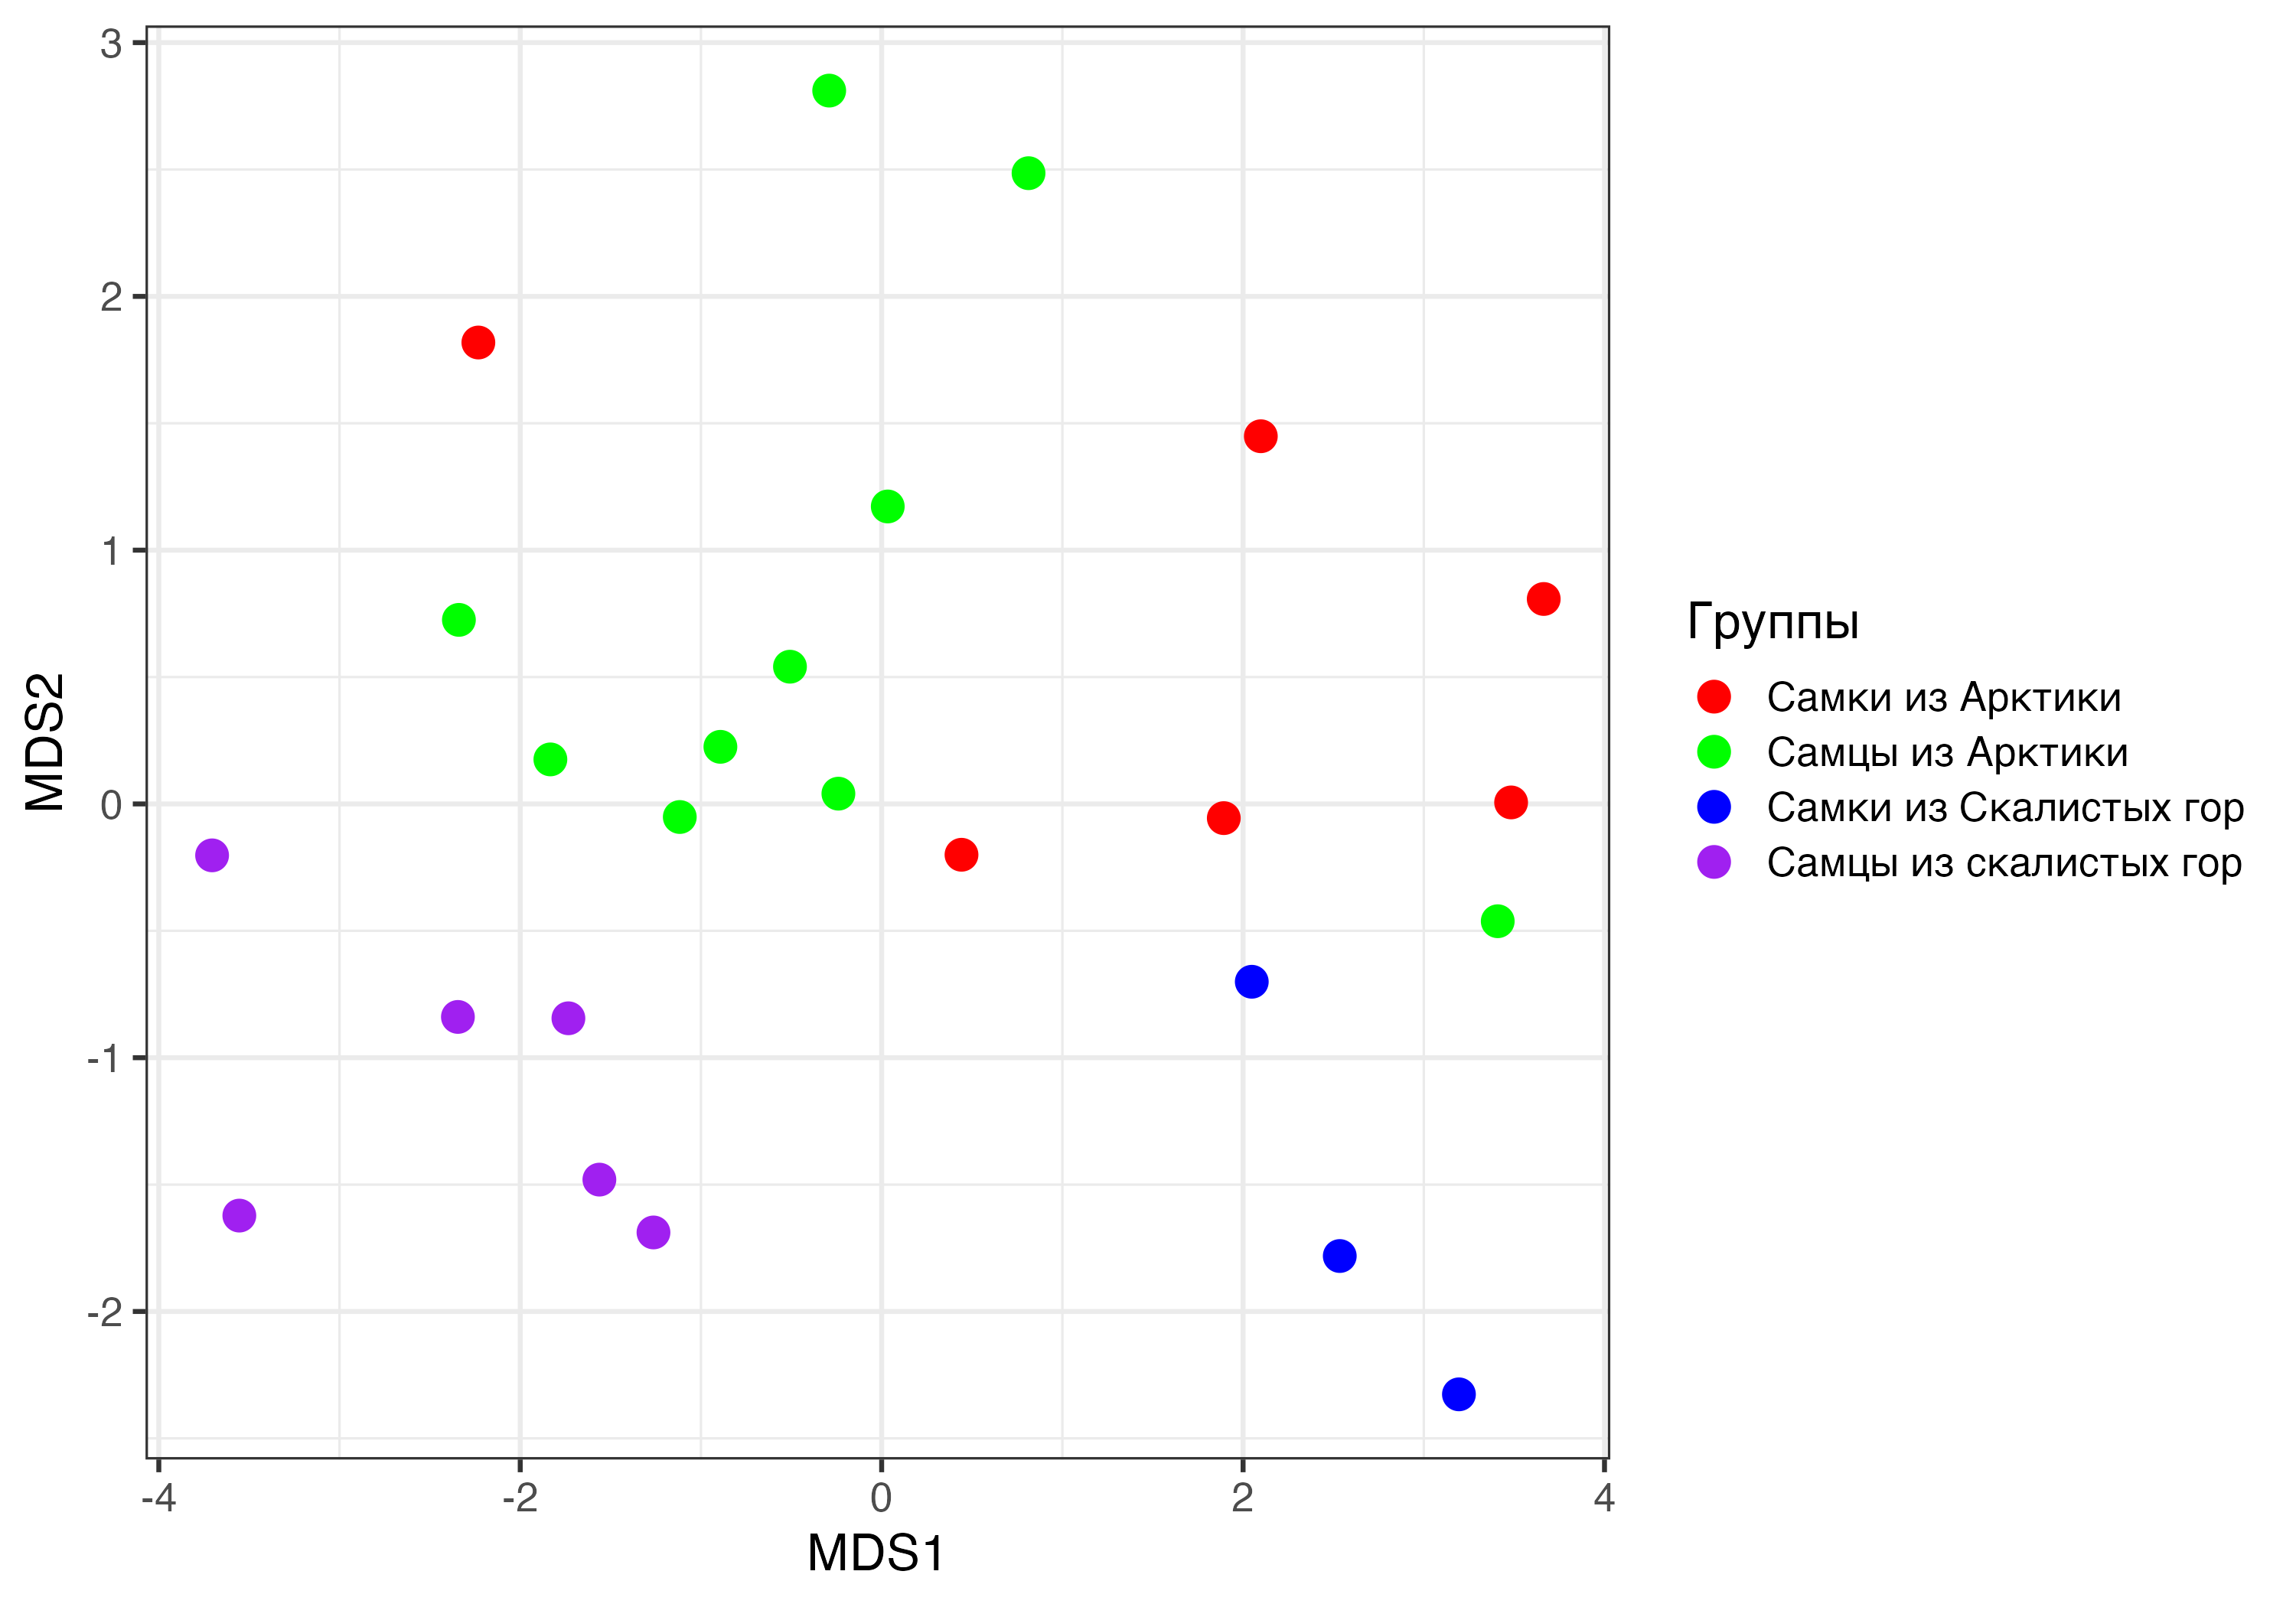
\includegraphics[keepaspectratio]{05_cluster_analysis_files/figure-beamer/unnamed-chunk-3-1.png}}
\end{frame}

\begin{frame}[fragile]{Решение}
\protect\phantomsection\label{ux440ux435ux448ux435ux43dux438ux435-1}
\tiny

\begin{Shaded}
\begin{Highlighting}[]
\FunctionTok{library}\NormalTok{(vegan)}
\FunctionTok{library}\NormalTok{(ggplot2); }\FunctionTok{theme\_set}\NormalTok{(}\FunctionTok{theme\_bw}\NormalTok{(}\AttributeTok{base\_size =} \DecValTok{16}\NormalTok{))}
\NormalTok{st\_w }\OtherTok{\textless{}{-}} \FunctionTok{scale}\NormalTok{(Wolves[, }\DecValTok{4}\SpecialCharTok{:}\FunctionTok{ncol}\NormalTok{(Wolves)]) }\DocumentationTok{\#\# стандартизируем}
\NormalTok{ord\_w }\OtherTok{\textless{}{-}} \FunctionTok{metaMDS}\NormalTok{(}\AttributeTok{comm =}\NormalTok{ st\_w, }\AttributeTok{distance =} \StringTok{"euclidean"}\NormalTok{, }\AttributeTok{autotransform =} \ConstantTok{FALSE}\NormalTok{)}
\NormalTok{dfr\_w }\OtherTok{\textless{}{-}} \FunctionTok{data.frame}\NormalTok{(ord\_w}\SpecialCharTok{$}\NormalTok{points, }\AttributeTok{Group =}\NormalTok{ Wolves}\SpecialCharTok{$}\NormalTok{group)}
\NormalTok{gg\_w }\OtherTok{\textless{}{-}} \FunctionTok{ggplot}\NormalTok{(dfr\_w, }\FunctionTok{aes}\NormalTok{(}\AttributeTok{x =}\NormalTok{ MDS1, }\AttributeTok{y =}\NormalTok{ MDS2)) }\SpecialCharTok{+} 
  \FunctionTok{geom\_point}\NormalTok{(}\FunctionTok{aes}\NormalTok{(}\AttributeTok{colour =}\NormalTok{ Group)) }\SpecialCharTok{+} 
  \FunctionTok{scale\_color\_manual}\NormalTok{(}\AttributeTok{labels =} \FunctionTok{c}\NormalTok{(}\StringTok{"Самки из Арктики"}\NormalTok{, }\StringTok{"Самцы из Арктики"}\NormalTok{,}
                                \StringTok{"Самки из Скалистых гор"}\NormalTok{, }
                                \StringTok{"Самцы из скалистых гор"}\NormalTok{), }
                      \AttributeTok{values =} \FunctionTok{c}\NormalTok{(}\StringTok{"red"}\NormalTok{, }\StringTok{"green"}\NormalTok{, }\StringTok{"blue"}\NormalTok{, }\StringTok{"purple"}\NormalTok{)) }\SpecialCharTok{+}
  \FunctionTok{labs}\NormalTok{(}\AttributeTok{colour =} \StringTok{"Группы"}\NormalTok{)}
\end{Highlighting}
\end{Shaded}

\begin{verbatim}
Run 0 stress 0.100972 
Run 1 stress 0.1433766 
Run 2 stress 0.100972 
... Procrustes: rmse 1.463843e-06  max resid 4.480716e-06 
... Similar to previous best
Run 3 stress 0.1267966 
Run 4 stress 0.100972 
... Procrustes: rmse 9.176626e-06  max resid 2.906529e-05 
... Similar to previous best
Run 5 stress 0.100972 
... New best solution
... Procrustes: rmse 5.45332e-06  max resid 1.826026e-05 
... Similar to previous best
Run 6 stress 0.1406304 
Run 7 stress 0.1380797 
Run 8 stress 0.1354586 
Run 9 stress 0.1345468 
Run 10 stress 0.1267966 
Run 11 stress 0.1406304 
Run 12 stress 0.1367748 
Run 13 stress 0.1274815 
Run 14 stress 0.1244479 
Run 15 stress 0.1367748 
Run 16 stress 0.1367748 
Run 17 stress 0.1244479 
Run 18 stress 0.1367494 
Run 19 stress 0.100972 
... Procrustes: rmse 8.753637e-06  max resid 2.974542e-05 
... Similar to previous best
Run 20 stress 0.1267966 
*** Best solution repeated 2 times
\end{verbatim}
\end{frame}

\begin{frame}{Методы кластеризации}
\protect\phantomsection\label{ux43cux435ux442ux43eux434ux44b-ux43aux43bux430ux441ux442ux435ux440ux438ux437ux430ux446ux438ux438}
\begin{columns}[T]
\begin{column}{0.5\linewidth}
\textbf{Иерархические методы}

\begin{itemize}
\tightlist
\item
  методы построения деревьев (о них следующие слайды)
\end{itemize}
\end{column}

\begin{column}{0.5\linewidth}
\textbf{Неиерархические методы}

\begin{itemize}
\tightlist
\item
  метод K-средних (K-means clustering)
\item
  метод нечёткой кластеризации C-средних (C-means clustering, fuzzy
  clustering)
\item
  Основанная на плотности пространственная кластеризация для приложений
  с шумами (Density-based spatial clustering of applications with noise,
  DBSCAN)
\end{itemize}
\end{column}
\end{columns}
\end{frame}

\begin{frame}{Какие бывают методы построения деревьев?}
\protect\phantomsection\label{ux43aux430ux43aux438ux435-ux431ux44bux432ux430ux44eux442-ux43cux435ux442ux43eux434ux44b-ux43fux43eux441ux442ux440ux43eux435ux43dux438ux44f-ux434ux435ux440ux435ux432ux44cux435ux432}
\textbf{Методы кластеризации на основании расстояний (о них сегодня)}

\begin{itemize}
\tightlist
\item
  Метод ближайшего соседа
\item
  Метод отдалённого соседа
\item
  Метод среднегруппового расстояния
\item
  Метод Варда
\item
  и т.д. и т.п.
\end{itemize}

\textbf{Методы кластеризации на основании признаков}

\begin{itemize}
\tightlist
\item
  Метод максимальной бережливости
\item
  Метод максимального правдоподобия
\end{itemize}

\textbf{И это еще далеко не всё!}
\end{frame}

\section{Методы кластеризации на основании
расстояний}\label{ux43cux435ux442ux43eux434ux44b-ux43aux43bux430ux441ux442ux435ux440ux438ux437ux430ux446ux438ux438-ux43dux430-ux43eux441ux43dux43eux432ux430ux43dux438ux438-ux440ux430ux441ux441ux442ux43eux44fux43dux438ux439}

\begin{frame}{Этапы кластеризации}
\protect\phantomsection\label{ux44dux442ux430ux43fux44b-ux43aux43bux430ux441ux442ux435ux440ux438ux437ux430ux446ux438ux438}
\begin{columns}[T]
\begin{column}{0.5\linewidth}
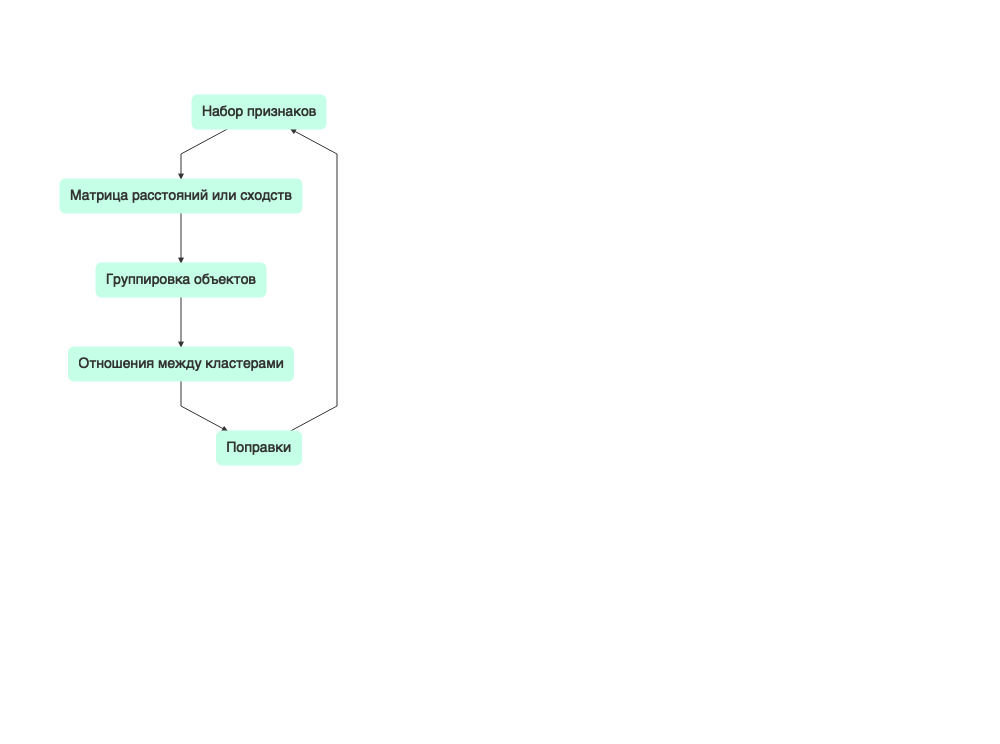
\includegraphics[width=2.5\linewidth,height=\textheight,keepaspectratio]{images/diagrammer_cluster.png}
\end{column}

\begin{column}{0.5\linewidth}
Результат кластеризации зависит от

\begin{itemize}
\tightlist
\item
  выбора признаков
\item
  коэффициента сходства-различия
\item
  от алгоритма кластеризации
\end{itemize}
\end{column}
\end{columns}
\end{frame}

\begin{frame}{Методы кластеризации}
\protect\phantomsection\label{ux43cux435ux442ux43eux434ux44b-ux43aux43bux430ux441ux442ux435ux440ux438ux437ux430ux446ux438ux438-1}
\begin{figure}

\centering{

\pandocbounded{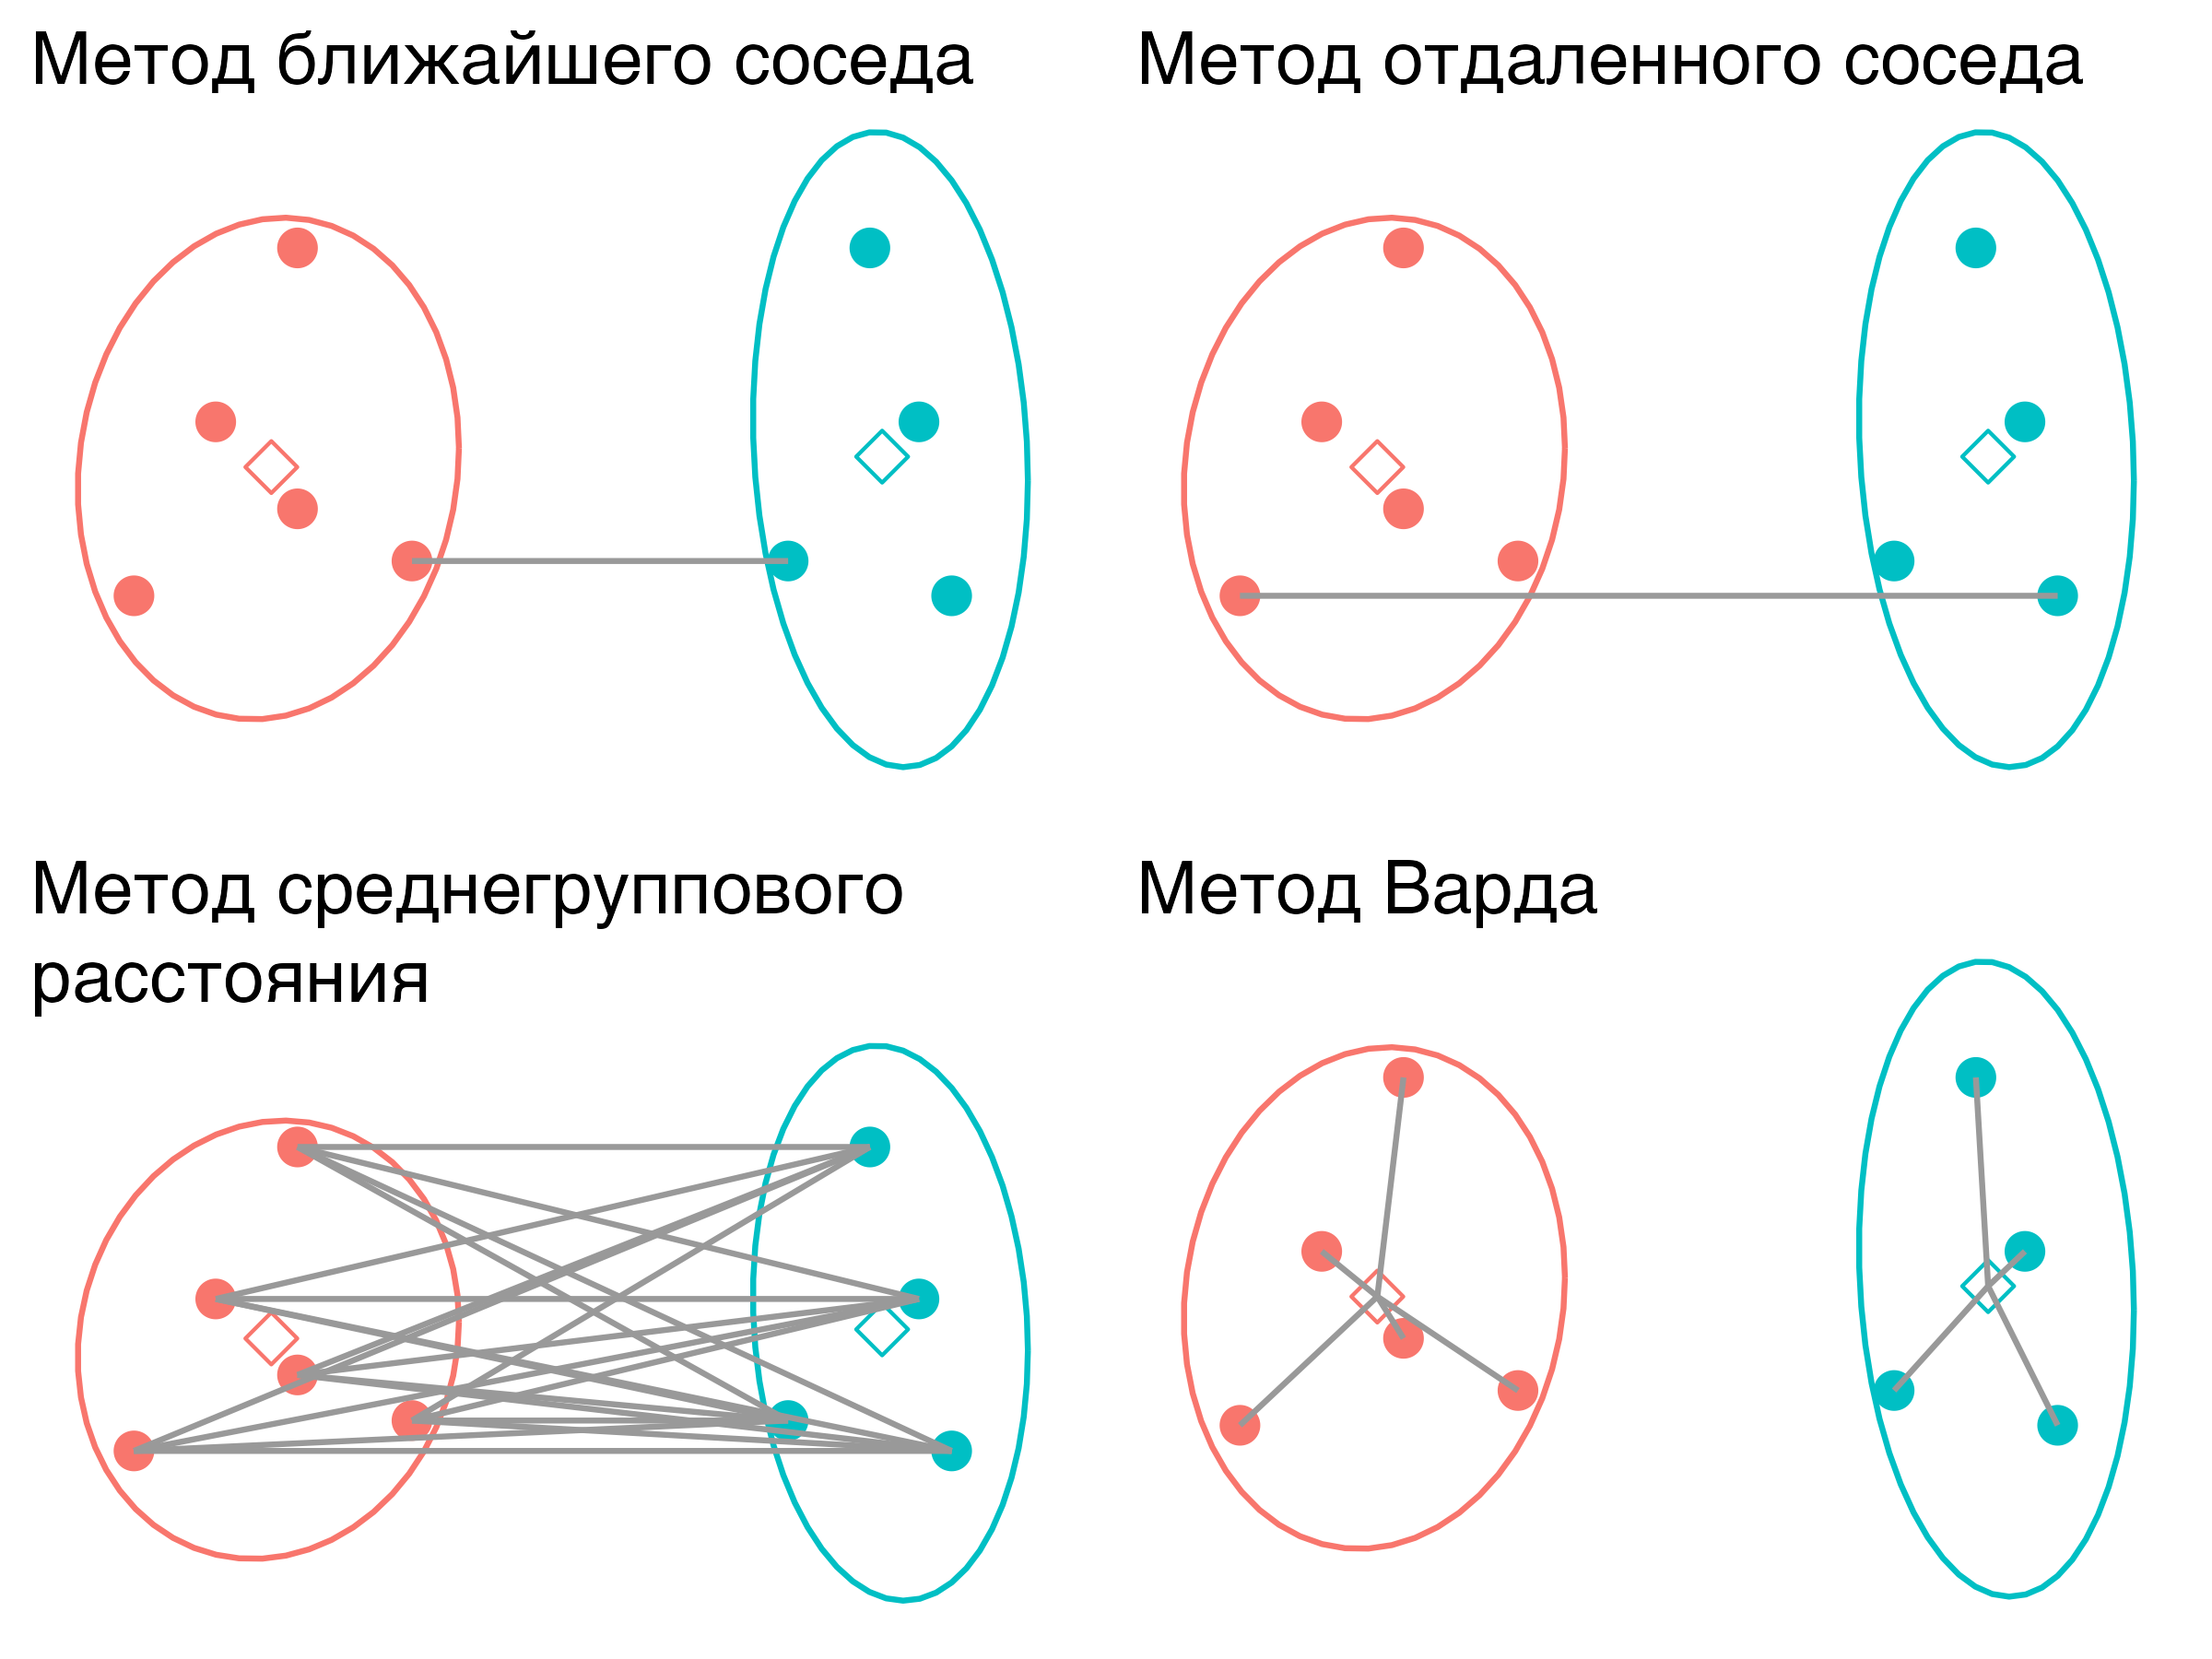
\includegraphics[keepaspectratio]{05_cluster_analysis_files/figure-beamer/fig-cluster-methods-1.png}}

}

\caption{\label{fig-cluster-methods}}

\end{figure}%
\end{frame}

\begin{frame}{Метод ближайшего соседа}
\protect\phantomsection\label{ux43cux435ux442ux43eux434-ux431ux43bux438ux436ux430ux439ux448ux435ux433ux43e-ux441ux43eux441ux435ux434ux430}
\begin{columns}[T]
\begin{column}{0.66\linewidth}
\textbf{= nearest neighbour = single linkage}

\begin{itemize}
\tightlist
\item
  к кластеру присоединяется ближайший к нему кластер/объект
\item
  кластеры объединяются в один на расстоянии, которое равно расстоянию
  между ближайшими объектами этих кластеров
\end{itemize}
\end{column}

\begin{column}{0.33\linewidth}
\begin{figure}

\centering{

\pandocbounded{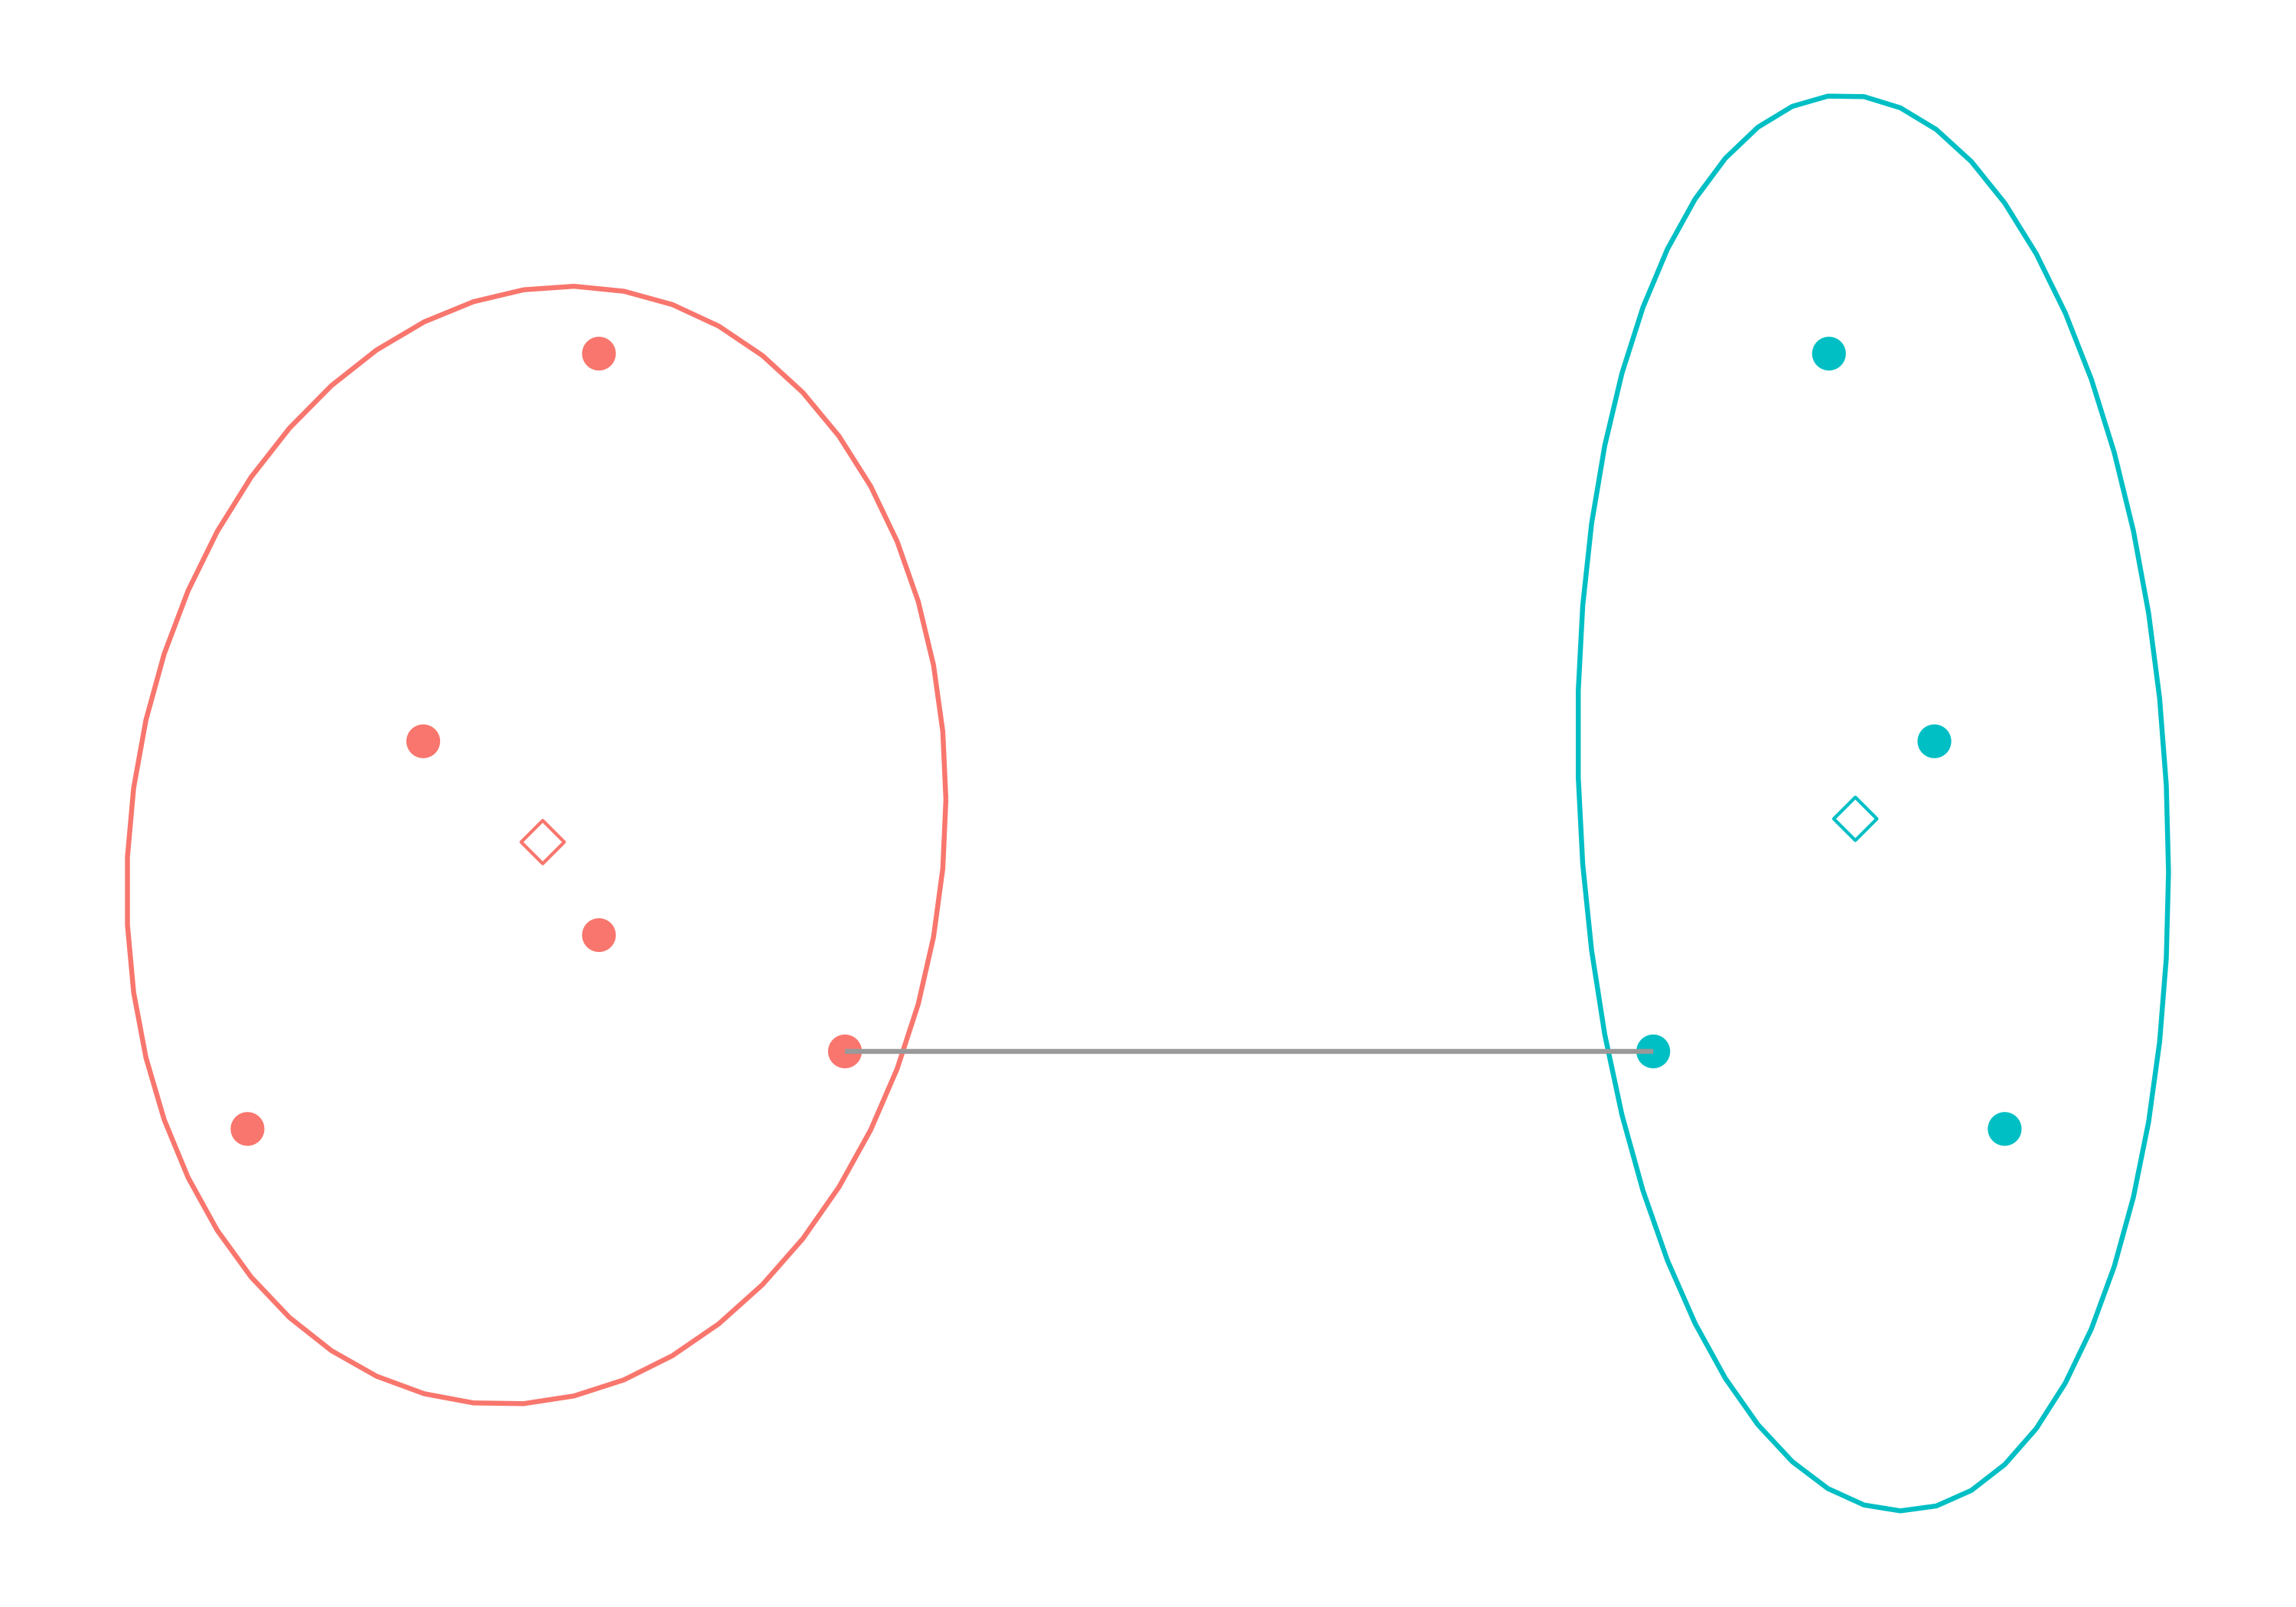
\includegraphics[keepaspectratio]{05_cluster_analysis_files/figure-beamer/fig-single-1.png}}

}

\caption{\label{fig-single}}

\end{figure}%
\end{column}
\end{columns}

\textbf{Особенности}

\begin{itemize}
\tightlist
\item
  Может быть сложно интерпретировать, если нужны группы

  \begin{itemize}
  \tightlist
  \item
    объекты на дендрограмме часто не образуют четко разделенных групп
  \item
    часто получаются цепочки кластеров (объекты присоединяются как бы по
    одному)
  \end{itemize}
\item
  Хорош для выявления градиентов
\end{itemize}
\end{frame}

\begin{frame}{Как работает метод ближайшего соседа}
\protect\phantomsection\label{ux43aux430ux43a-ux440ux430ux431ux43eux442ux430ux435ux442-ux43cux435ux442ux43eux434-ux431ux43bux438ux436ux430ux439ux448ux435ux433ux43e-ux441ux43eux441ux435ux434ux430}
\begin{columns}[T]
\begin{column}{0.7\linewidth}
\begin{figure}

\centering{

\pandocbounded{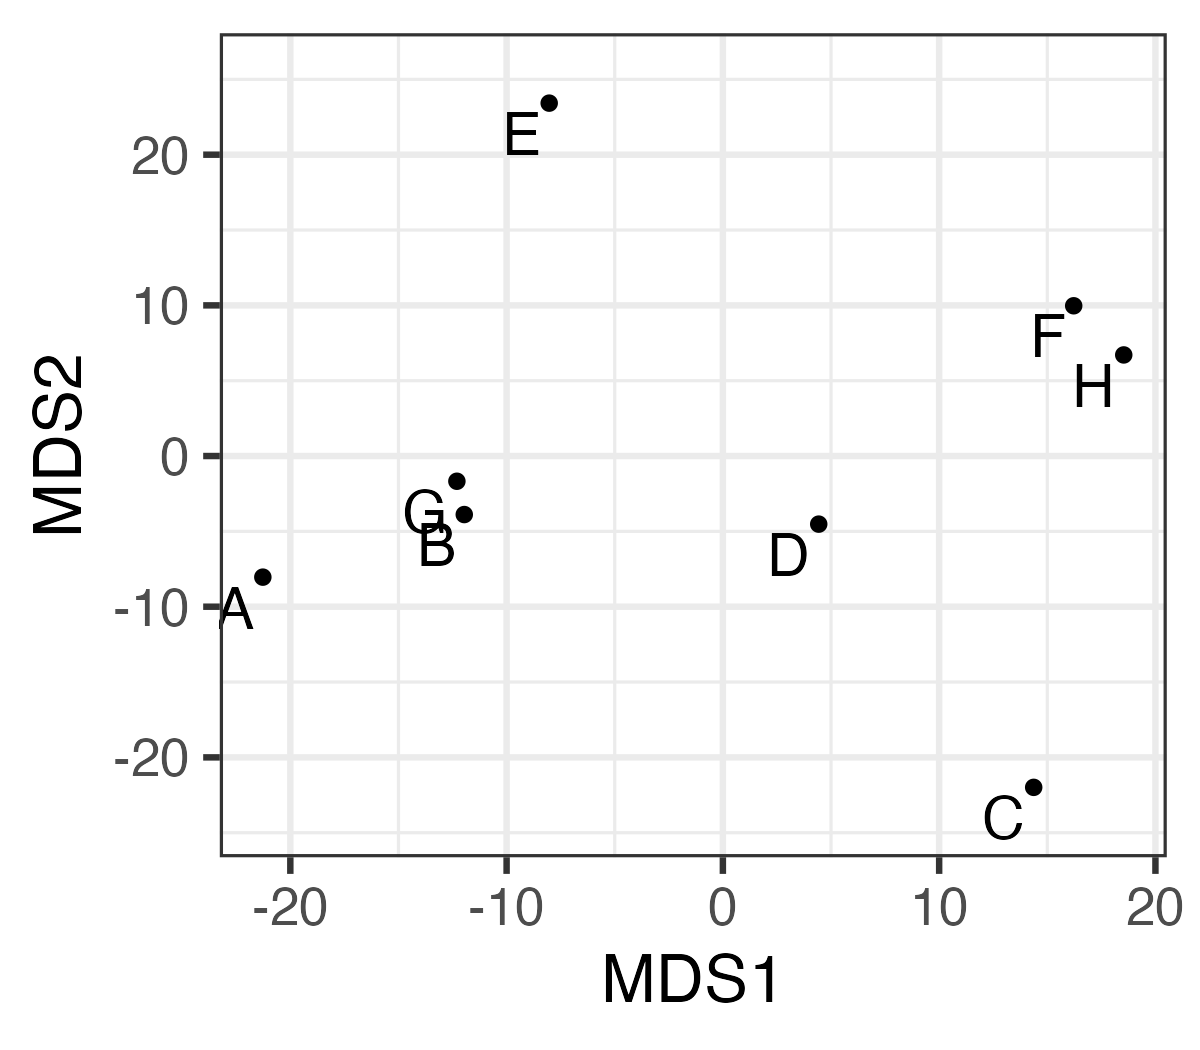
\includegraphics[keepaspectratio]{05_cluster_analysis_files/figure-beamer/fig-single-guess-1.png}}

}

\caption{\label{fig-single-guess}}

\end{figure}%
\end{column}

\begin{column}{0.3\linewidth}
Анимация --- в короткой .pptx презентации.
\end{column}
\end{columns}
\end{frame}

\begin{frame}{Метод отдаленного соседа}
\protect\phantomsection\label{ux43cux435ux442ux43eux434-ux43eux442ux434ux430ux43bux435ux43dux43dux43eux433ux43e-ux441ux43eux441ux435ux434ux430}
\begin{columns}[T]
\begin{column}{0.6\linewidth}
\textbf{= furthest neighbour = complete linkage}

\begin{itemize}
\tightlist
\item
  к кластеру присоединяется отдаленный кластер/объект
\item
  кластеры объединяются в один на расстоянии, которое равно расстоянию
  между самыми отдаленными объектами этих кластеров (следствие --- чем
  более крупная группа, тем сложнее к ней присоединиться)
\end{itemize}
\end{column}

\begin{column}{0.4\linewidth}
\begin{figure}

\centering{

\pandocbounded{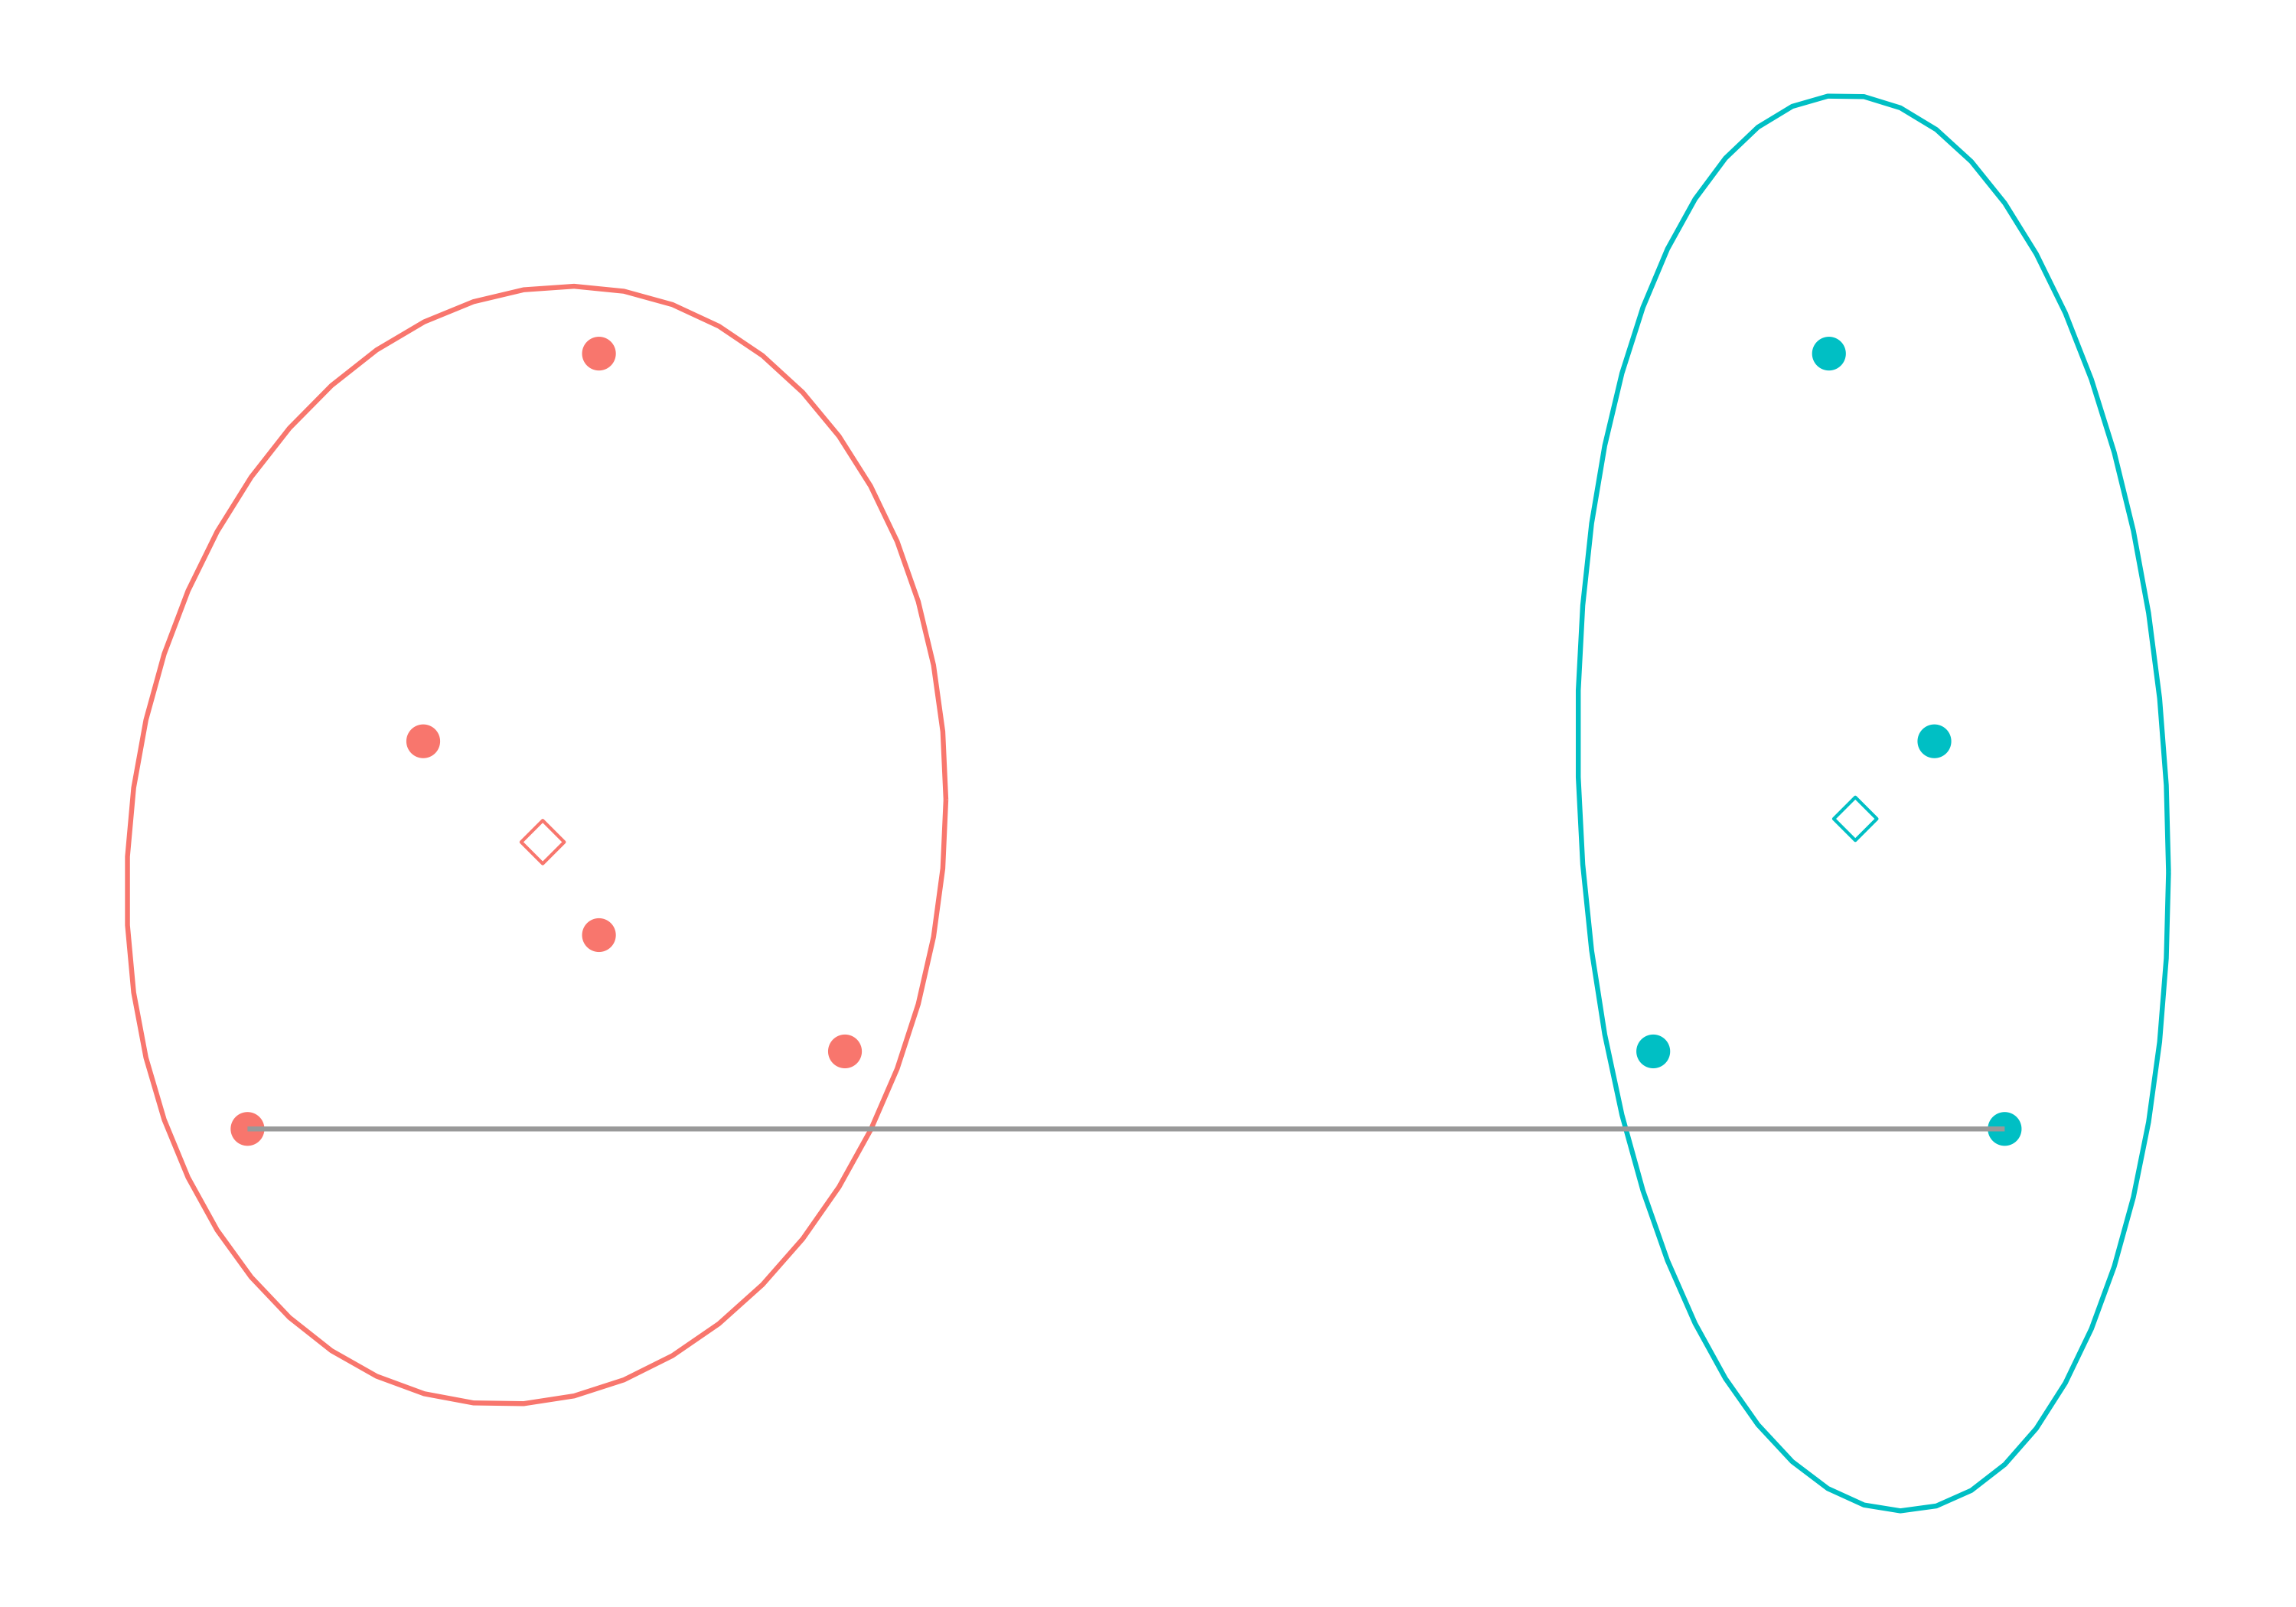
\includegraphics[keepaspectratio]{05_cluster_analysis_files/figure-beamer/fig-complete-1.png}}

}

\caption{\label{fig-complete}}

\end{figure}%
\end{column}
\end{columns}

\textbf{Особенности}

\begin{itemize}
\tightlist
\item
  На дендрограмме образуется много отдельных некрупных групп
\item
  Хорош для поиска дискретных групп в данных
\end{itemize}
\end{frame}

\begin{frame}{Как работает метод отдаленного соседа}
\protect\phantomsection\label{ux43aux430ux43a-ux440ux430ux431ux43eux442ux430ux435ux442-ux43cux435ux442ux43eux434-ux43eux442ux434ux430ux43bux435ux43dux43dux43eux433ux43e-ux441ux43eux441ux435ux434ux430}
\begin{figure}

\centering{

\pandocbounded{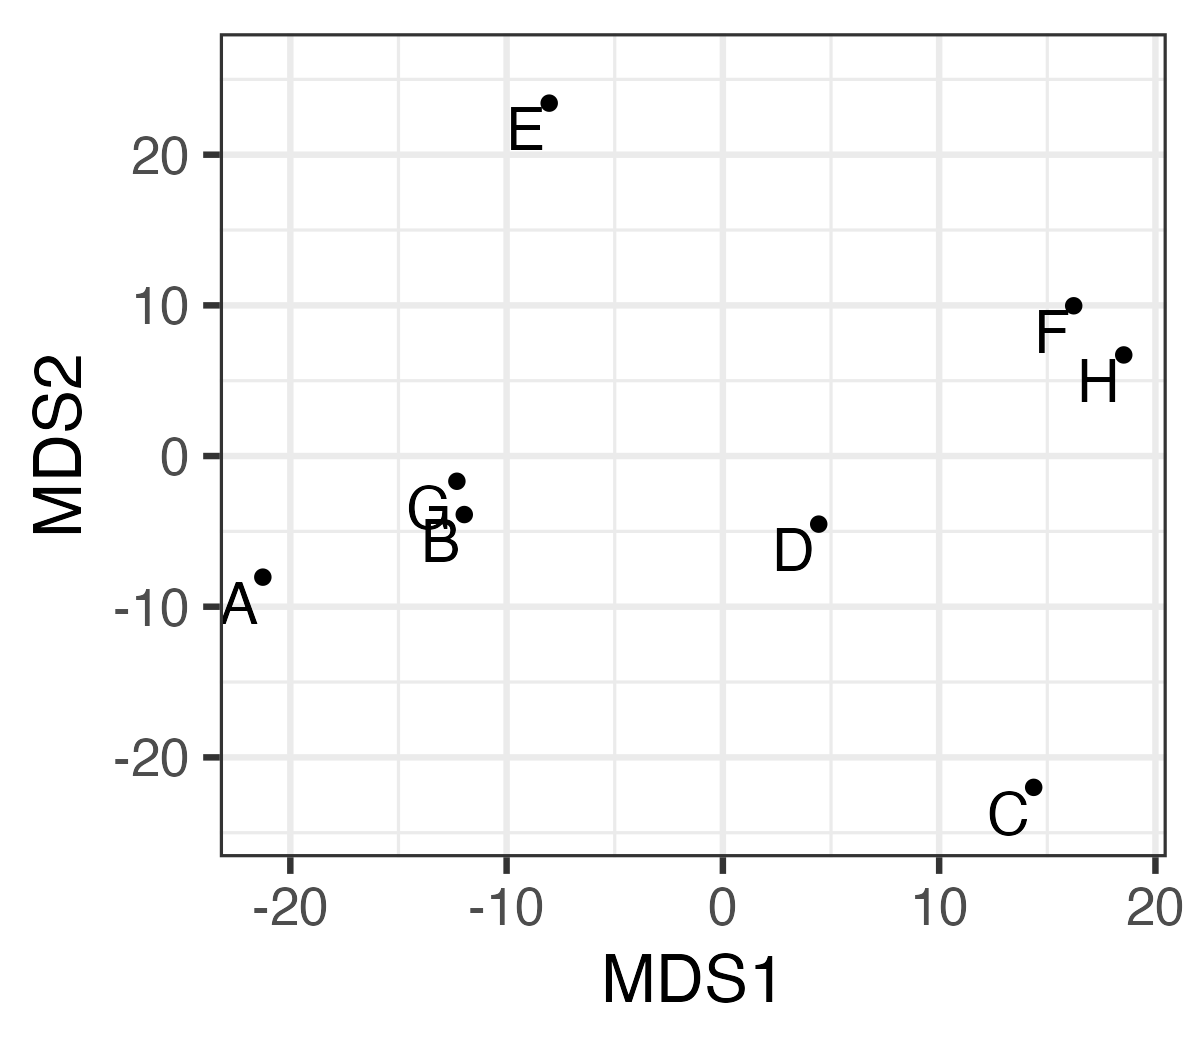
\includegraphics[keepaspectratio]{05_cluster_analysis_files/figure-beamer/fig-complete-guess-1.png}}

}

\caption{\label{fig-complete-guess}}

\end{figure}%
\end{frame}

\begin{frame}{Метод невзвешенного попарного среднего}
\protect\phantomsection\label{ux43cux435ux442ux43eux434-ux43dux435ux432ux437ux432ux435ux448ux435ux43dux43dux43eux433ux43e-ux43fux43eux43fux430ux440ux43dux43eux433ux43e-ux441ux440ux435ux434ux43dux435ux433ux43e}
\begin{columns}[T]
\begin{column}{0.66\linewidth}
\begin{block}{}

\textbf{= UPGMA = Unweighted Pair Group Method with Arithmetic mean}

кластеры объединяются в один на расстоянии, которое равно среднему значению всех возможных расстояний между объектами из разных кластеров.
\end{block}
\end{column}

\begin{column}{0.33\linewidth}
\begin{figure}

\centering{

\pandocbounded{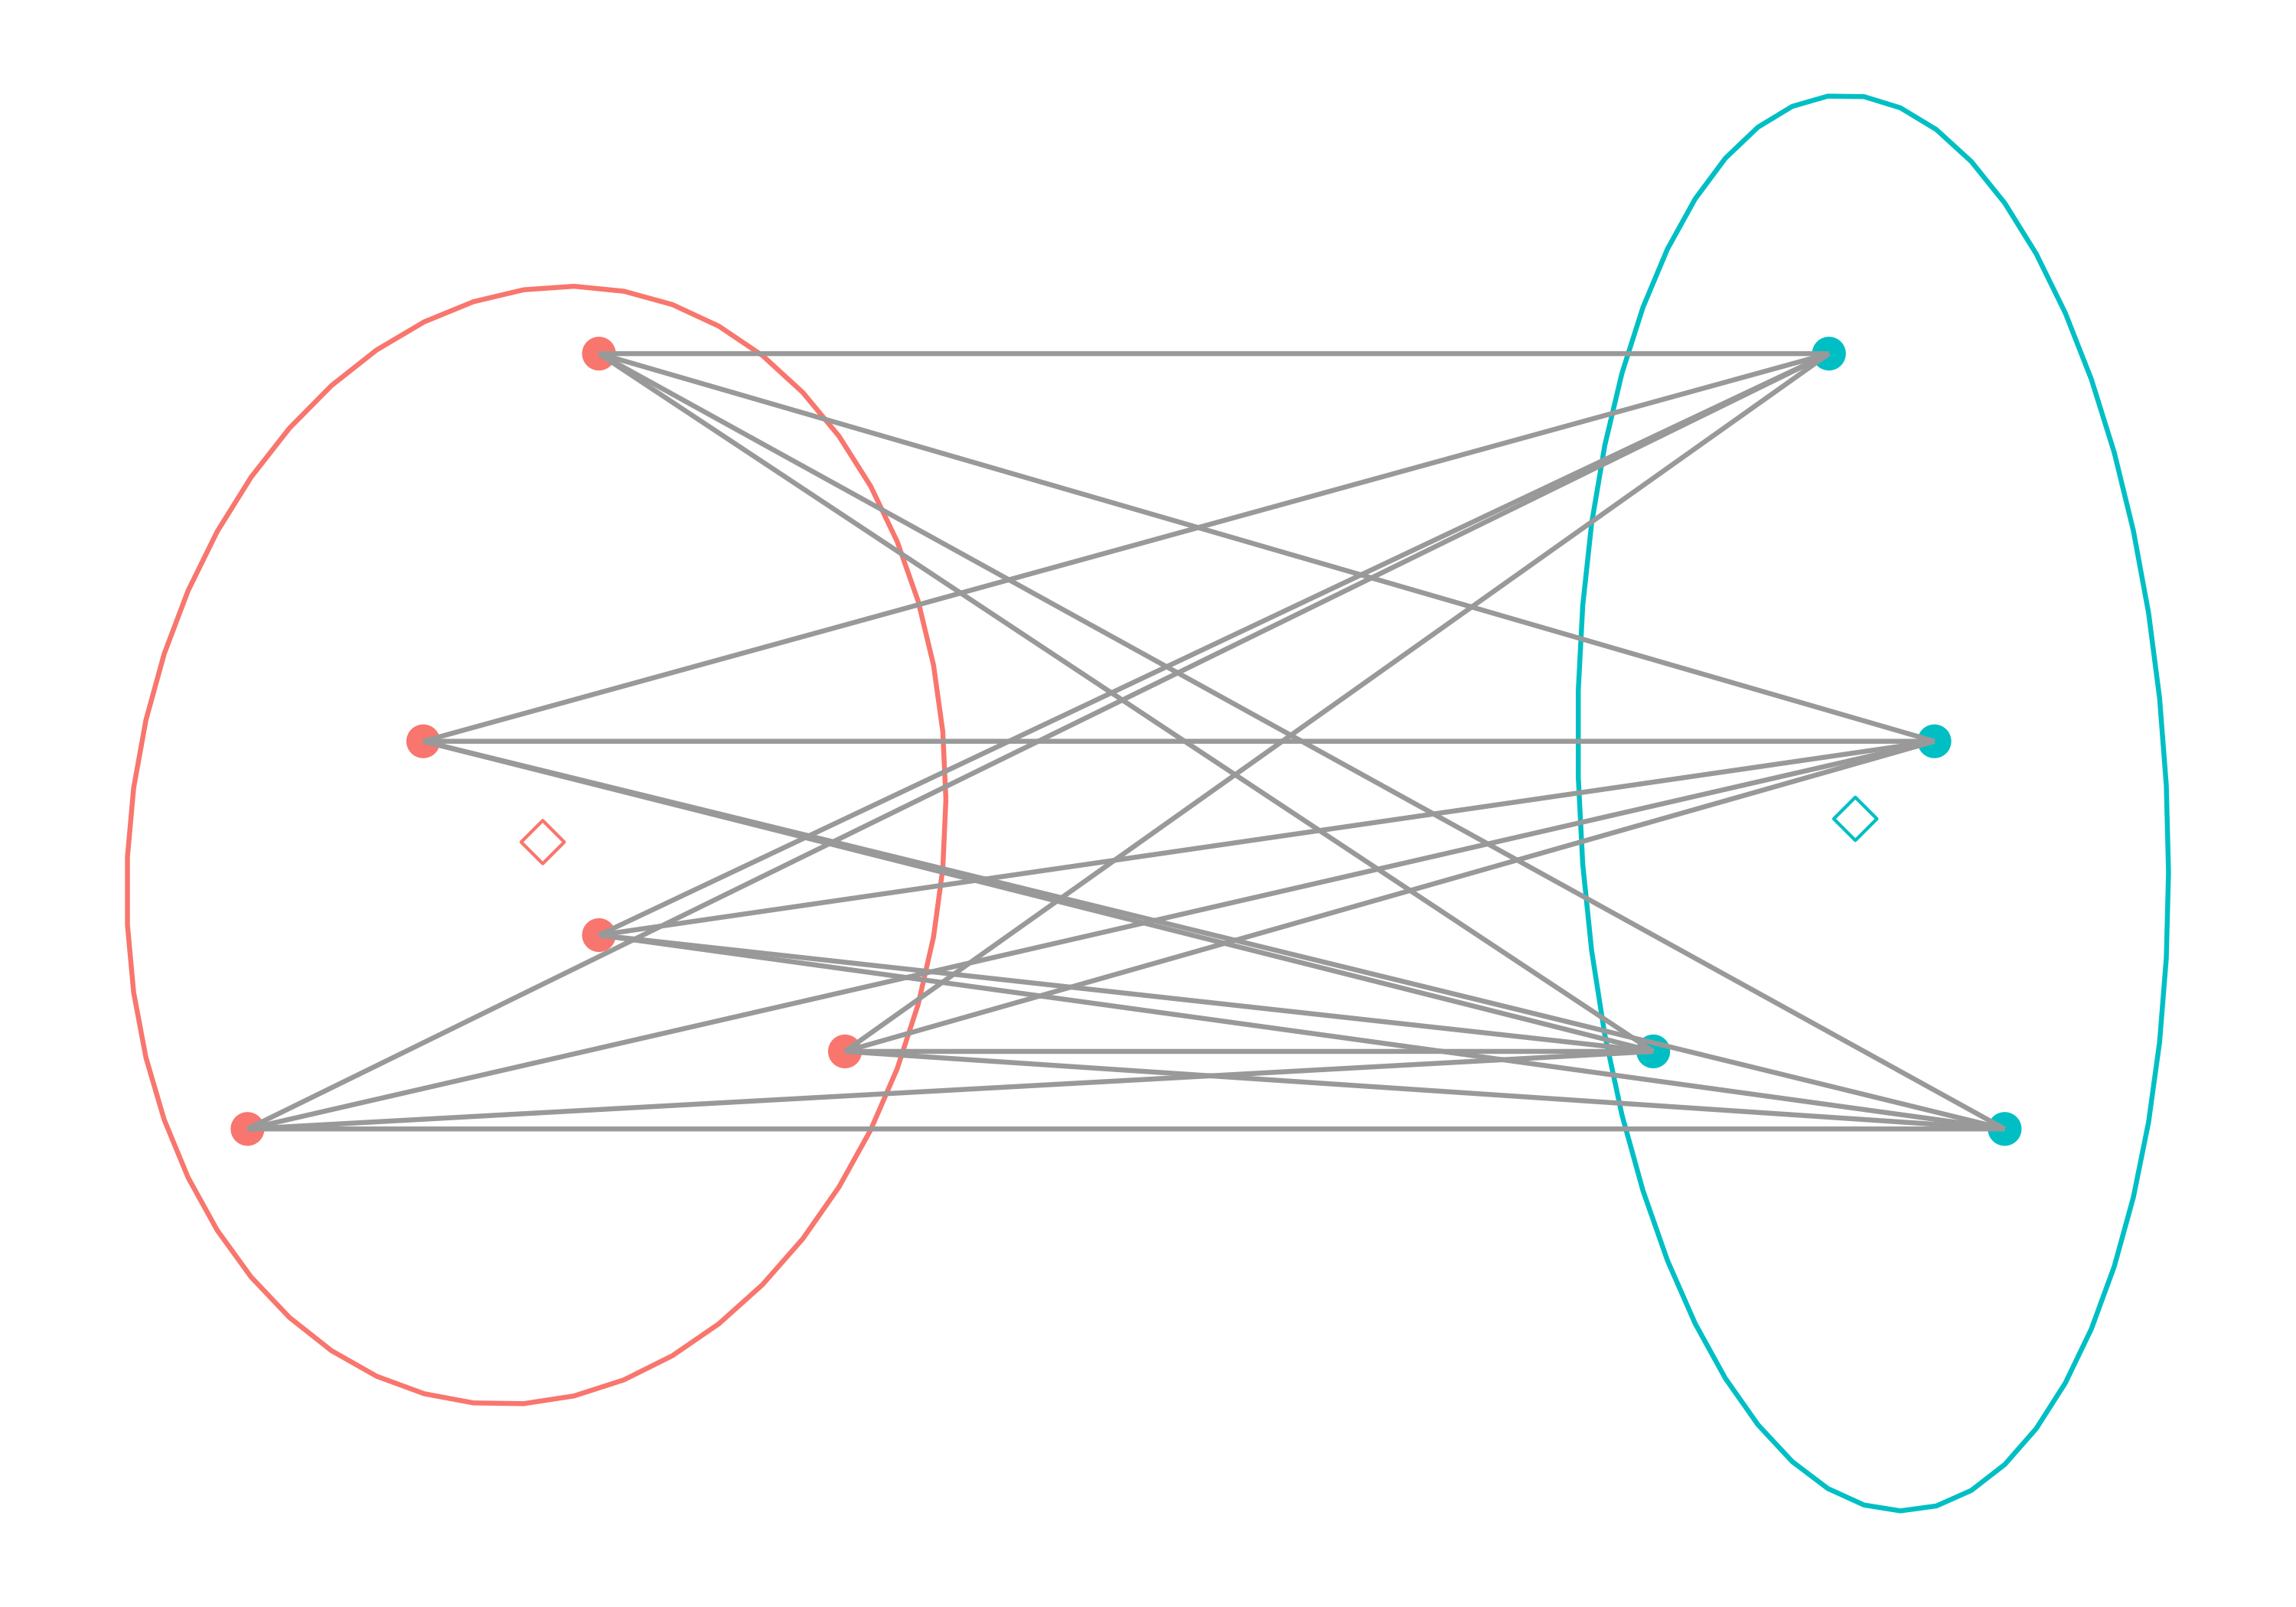
\includegraphics[keepaspectratio]{05_cluster_analysis_files/figure-beamer/fig-average-1.png}}

}

\caption{\label{fig-average}}

\end{figure}%
\end{column}
\end{columns}

\textbf{Особенности}

UPGMA и WPGMA иногда могут приводить к инверсиям на дендрограммах.

\begin{columns}[T]
\begin{column}{0.66\linewidth}
\begin{figure}[H]

{\centering \includegraphics[width=0.6\linewidth,height=\textheight,keepaspectratio]{images/clust-revert.png}

}

\caption{Инверсии на дендрограммах}

\end{figure}%
\end{column}

\begin{column}{0.33\linewidth}
из Borcard et al., 2011
\end{column}
\end{columns}
\end{frame}

\begin{frame}{UPGMA и WPGMA}
\protect\phantomsection\label{upgma-ux438-wpgma}
\begin{columns}[T]
\begin{column}{0.5\linewidth}
UPGMA --- \textbf{Unweighted} Pair Group Method with Arithmetic mean

Дистанция между кластерами рассчитывается:

\[d_{(AB),C} = \frac{n_A \cdot d_{A,C} + n_B \cdot d_{B,C}}{n_A + n_B}\]
\end{column}

\begin{column}{0.5\linewidth}
WPGMA --- \textbf{Weighted} Pair Group Method with Arithmetic mean

Дистанция между кластерами рассчитывается:

\[d_{(AB),C} = \frac{d_{A,C} + d_{B,C}}{2}\]

Взвешенный не потому, что задаются разные веса при кластеризации, а
поскольку исходные расстояния оказывают неравное влияние на результат
--- побочный эффект игнорирования размера кластеров при расчете
расстояния.
\end{column}
\end{columns}
\end{frame}

\begin{frame}{Как работает метод среднегруппового расстояния}
\protect\phantomsection\label{ux43aux430ux43a-ux440ux430ux431ux43eux442ux430ux435ux442-ux43cux435ux442ux43eux434-ux441ux440ux435ux434ux43dux435ux433ux440ux443ux43fux43fux43eux432ux43eux433ux43e-ux440ux430ux441ux441ux442ux43eux44fux43dux438ux44f}
\pandocbounded{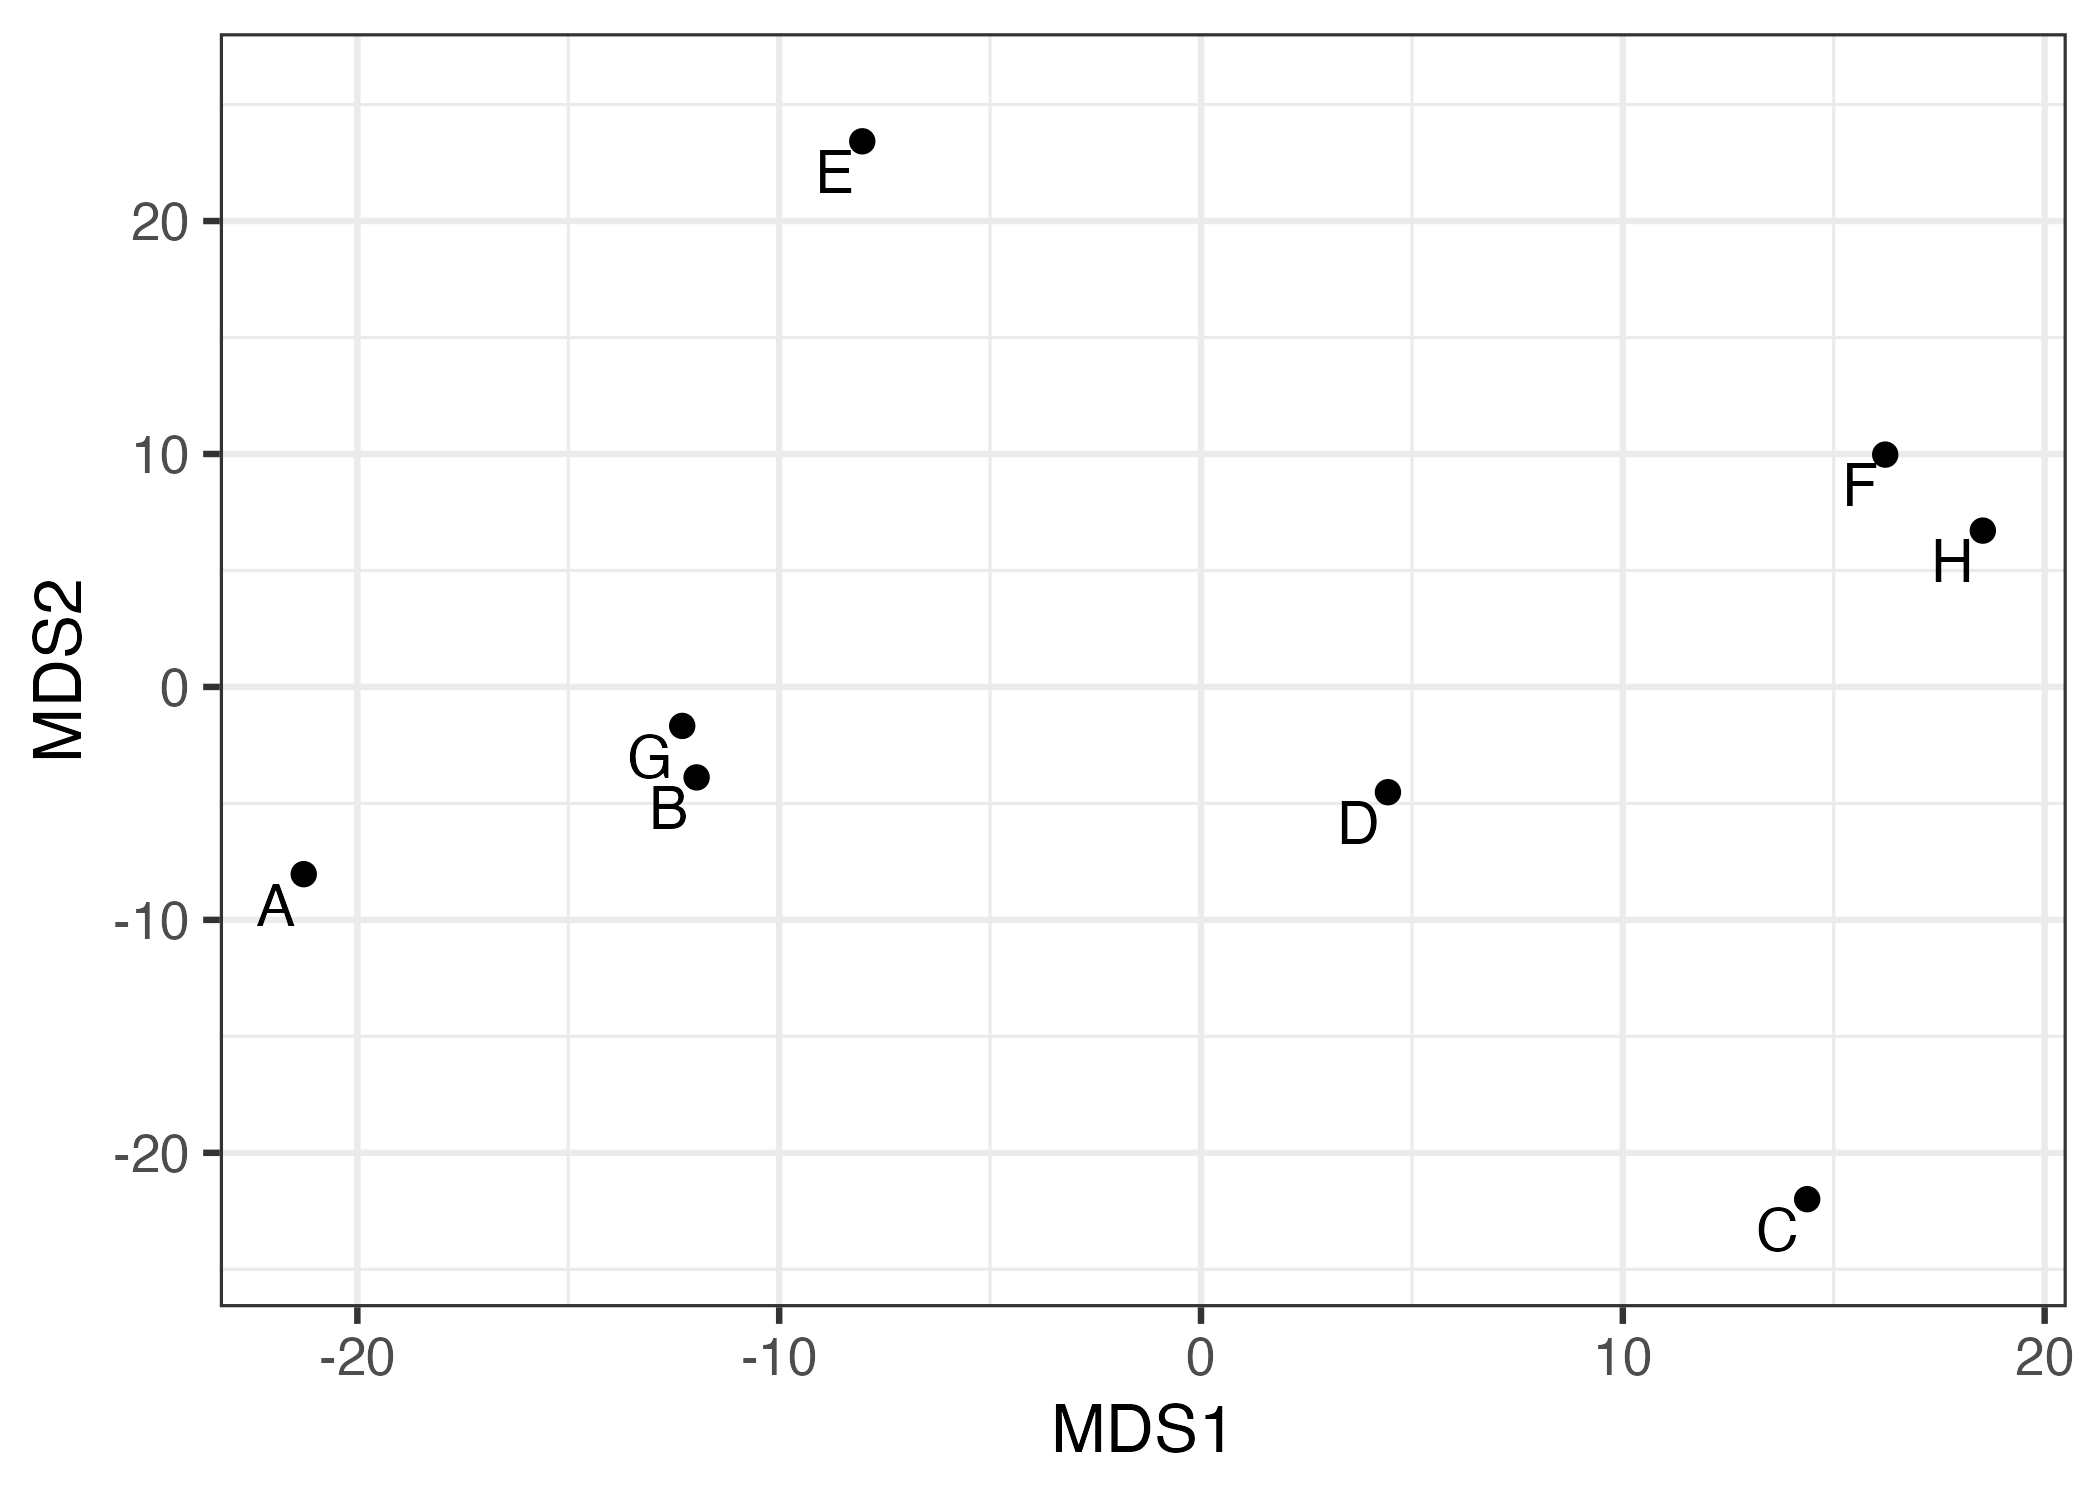
\includegraphics[keepaspectratio]{05_cluster_analysis_files/figure-beamer/average-guess-1.png}}
\end{frame}

\begin{frame}{Метод Варда}
\protect\phantomsection\label{ux43cux435ux442ux43eux434-ux432ux430ux440ux434ux430}
\begin{columns}[T]
\begin{column}{0.6\linewidth}
\begin{block}{}

\textbf{= Ward's Minimum Variance Clustering}

объекты объединяются в кластеры так, чтобы внутригрупповая дисперсия расстояний была минимальной.
\end{block}

\begin{figure}

\centering{

\pandocbounded{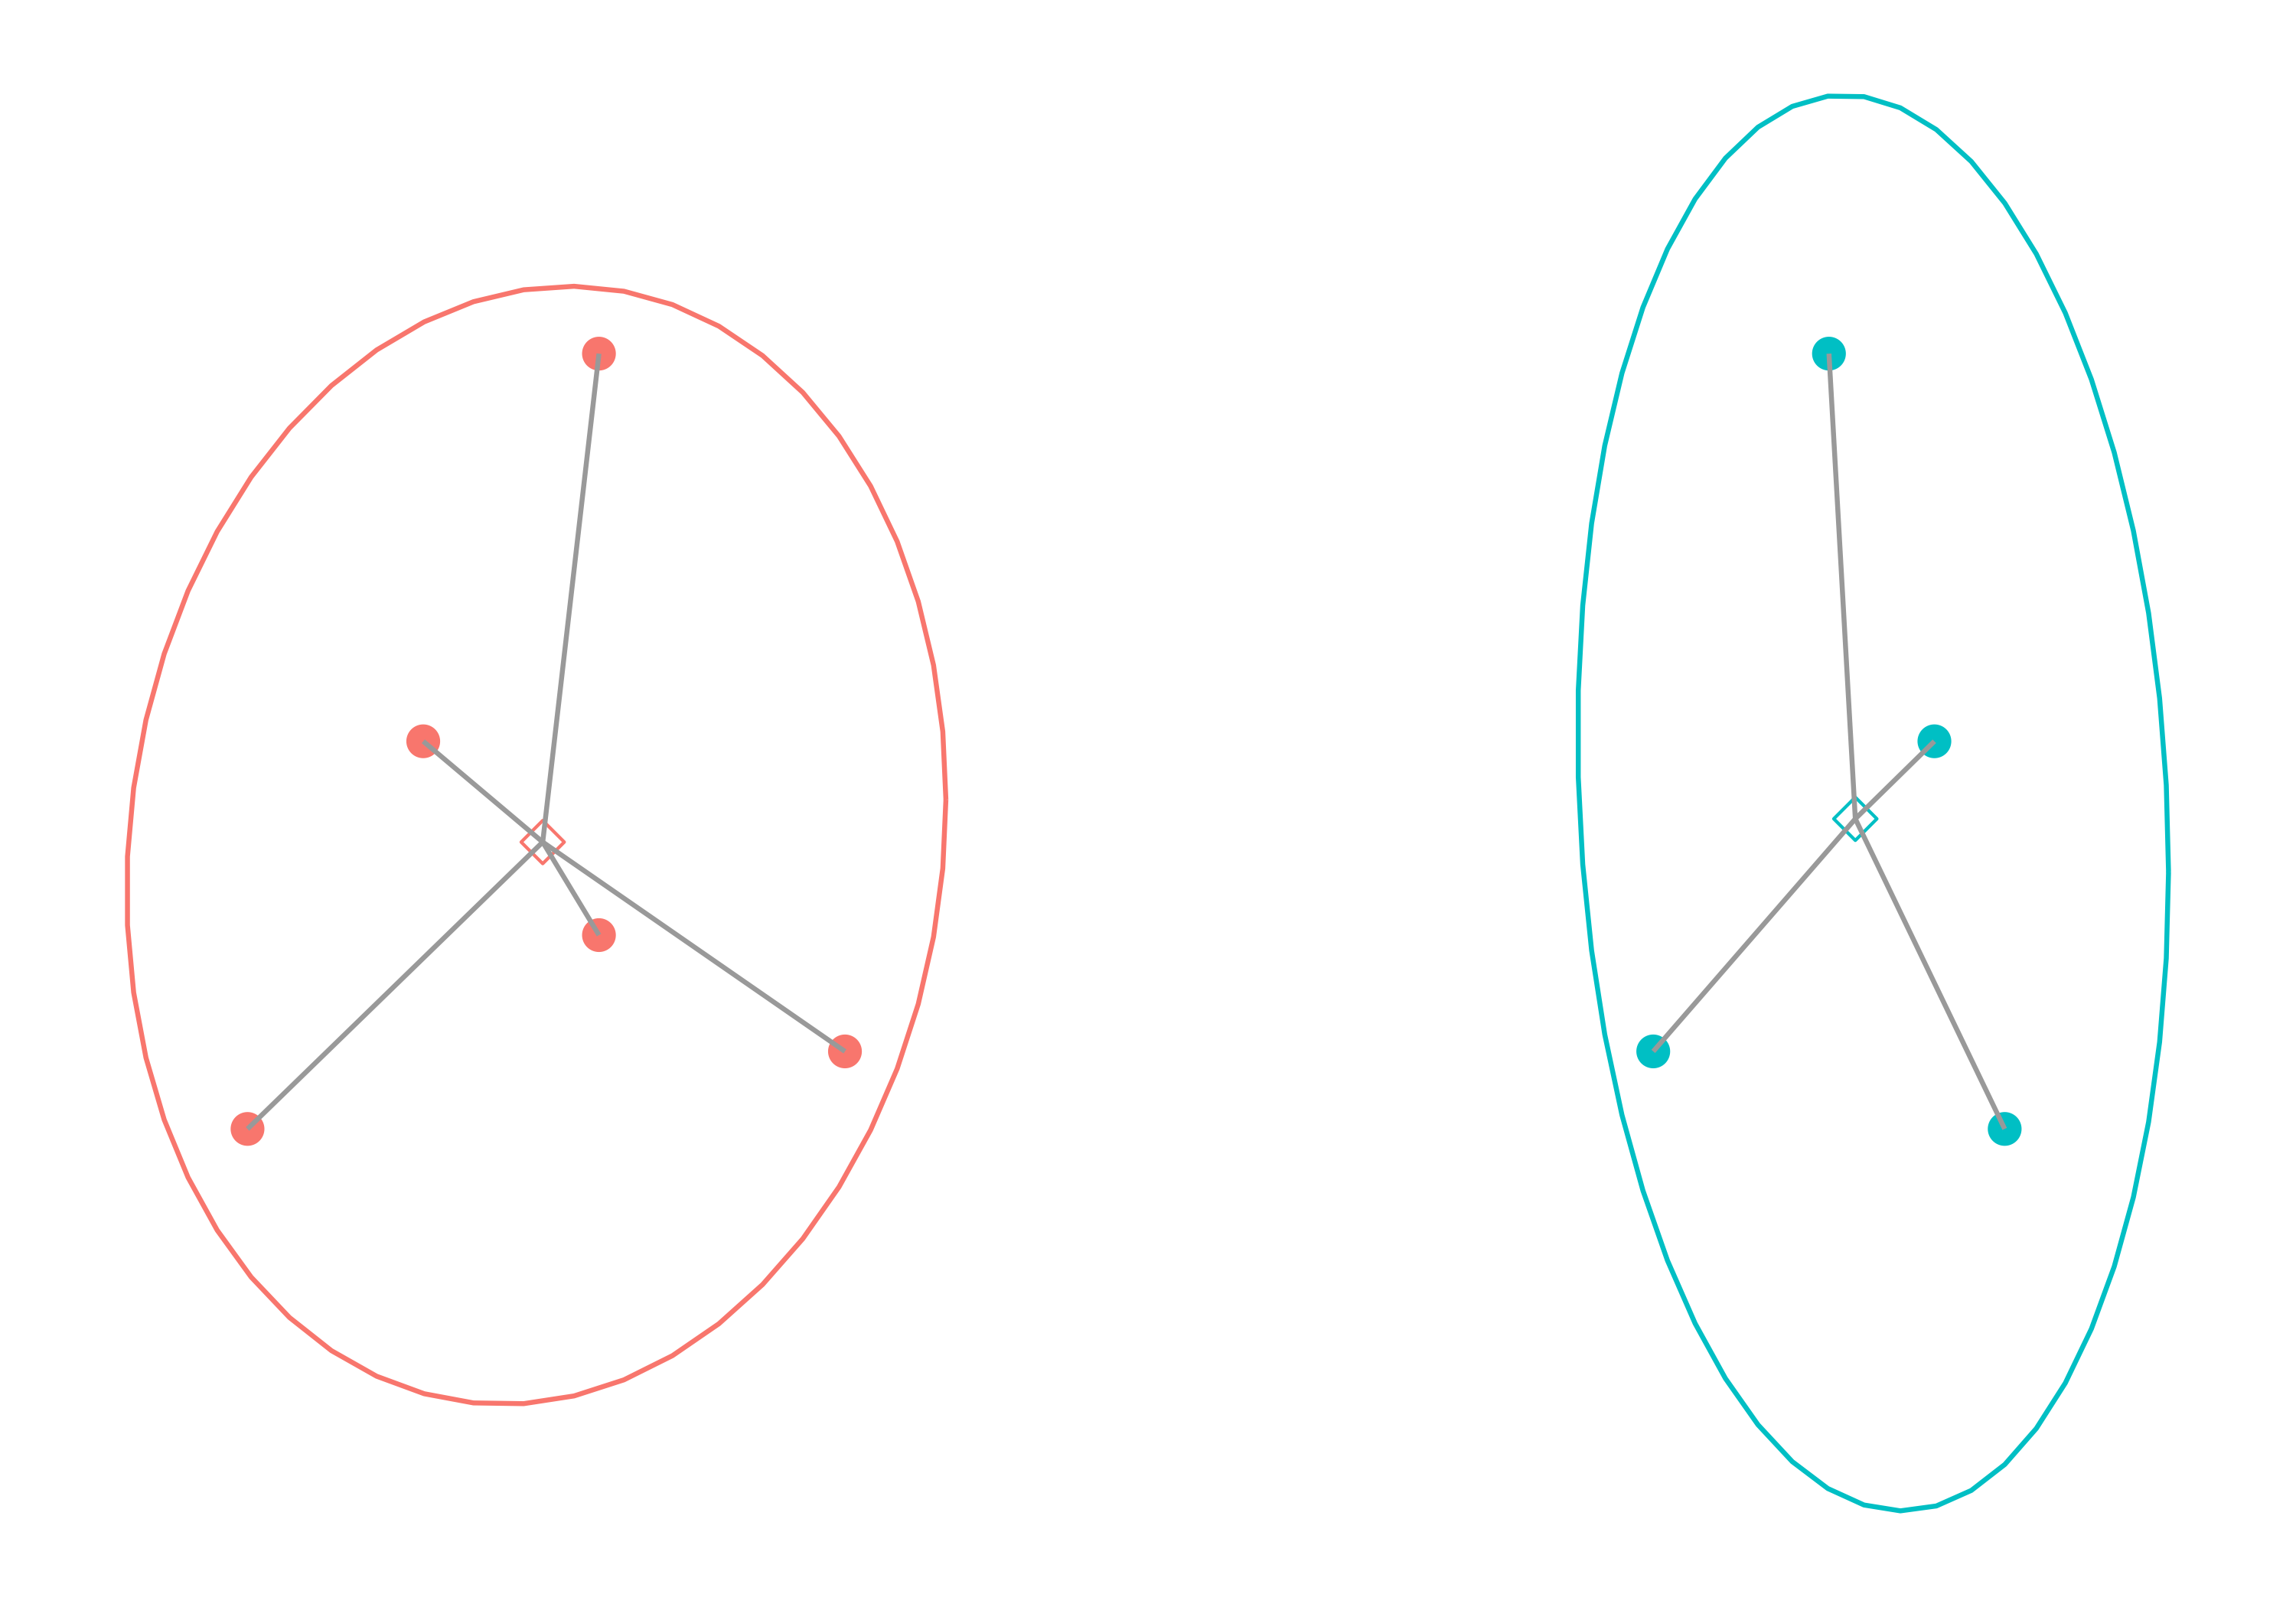
\includegraphics[keepaspectratio]{05_cluster_analysis_files/figure-beamer/fig-ward-1.png}}

}

\caption{\label{fig-ward}}

\end{figure}%
\end{column}

\begin{column}{0.33\linewidth}
\textbf{Особенности}

метод годится и для неевклидовых расстояний несмотря на то, что
внутригрупповая дисперсия расстояний рассчитывается так, как будто это
евклидовы расстояния.
\end{column}
\end{columns}
\end{frame}

\begin{frame}{Как работает метод Варда}
\protect\phantomsection\label{ux43aux430ux43a-ux440ux430ux431ux43eux442ux430ux435ux442-ux43cux435ux442ux43eux434-ux432ux430ux440ux434ux430}
\pandocbounded{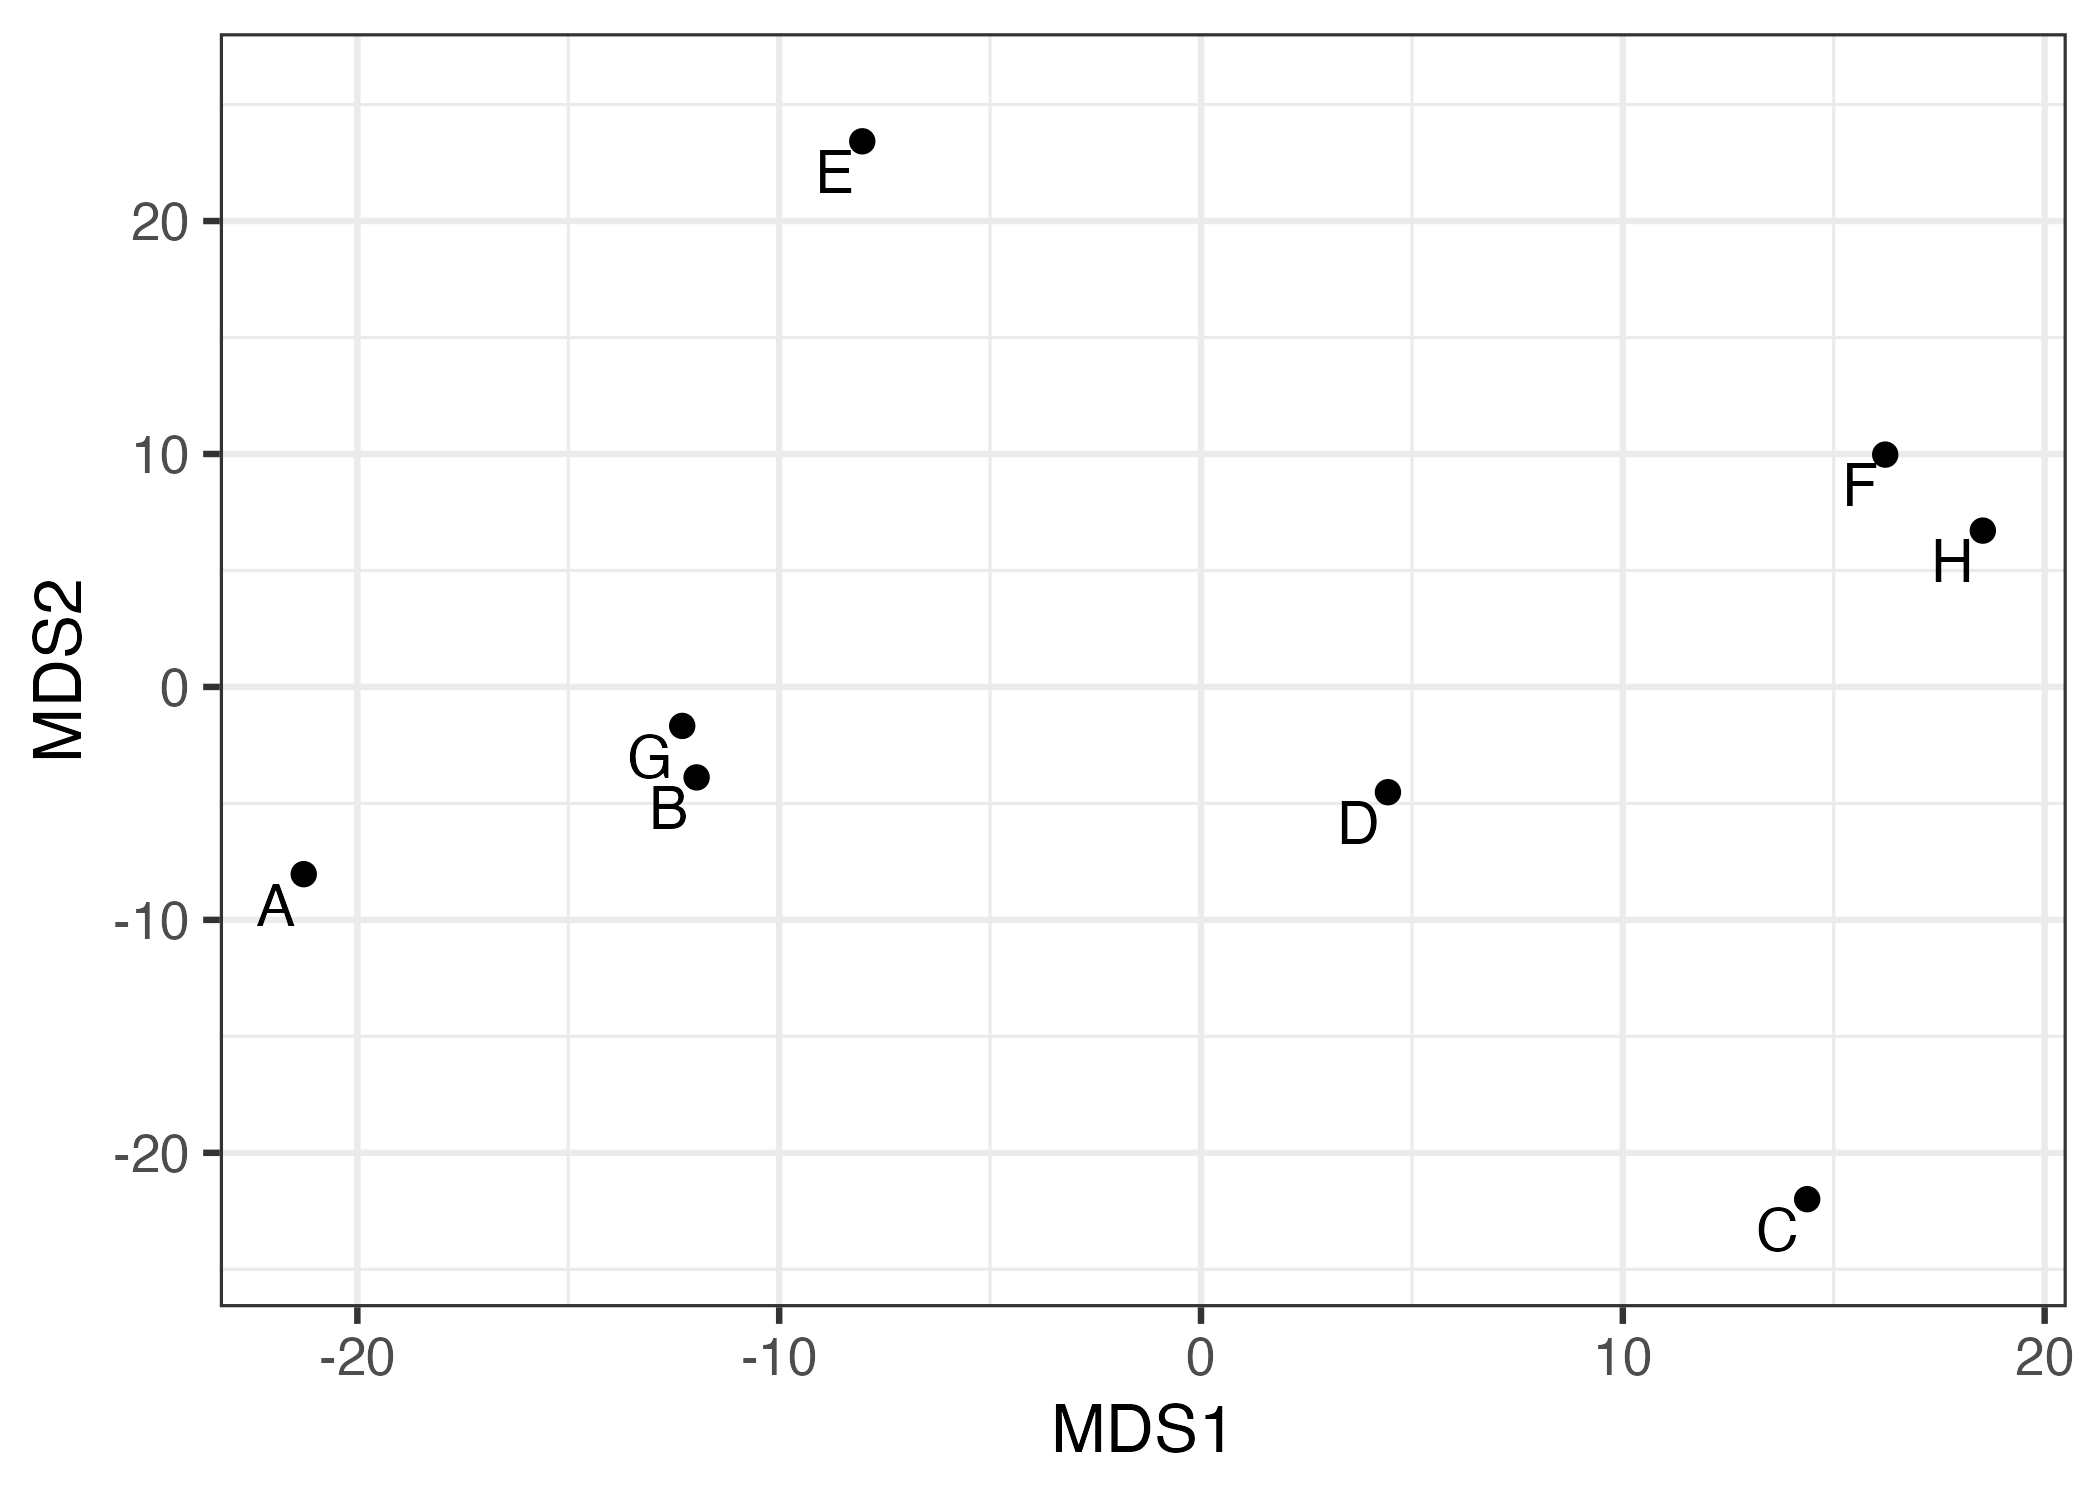
\includegraphics[keepaspectratio]{05_cluster_analysis_files/figure-beamer/ward-guess-1.png}}
\end{frame}

\section{Кластерный анализ в
R}\label{ux43aux43bux430ux441ux442ux435ux440ux43dux44bux439-ux430ux43dux430ux43bux438ux437-ux432-r}

\begin{frame}[fragile]{Кластеризация}
\protect\phantomsection\label{ux43aux43bux430ux441ux442ux435ux440ux438ux437ux430ux446ux438ux44f}
Давайте построим деревья при помощи нескольких алгоритмов кластеризации
(по стандартизованным данным, с использованием Евклидова расстояния) и
сравним их.

\begin{Shaded}
\begin{Highlighting}[]
\CommentTok{\# Пакеты для визуализации кластеризации}
\FunctionTok{library}\NormalTok{(ape)}
\FunctionTok{library}\NormalTok{(dendextend)}
\end{Highlighting}
\end{Shaded}

\begin{Shaded}
\begin{Highlighting}[]
\CommentTok{\# Матрица расстояний}
\NormalTok{d }\OtherTok{\textless{}{-}} \FunctionTok{dist}\NormalTok{(}\AttributeTok{x =}\NormalTok{ st\_w, }\AttributeTok{method =} \StringTok{"euclidean"}\NormalTok{)}
\end{Highlighting}
\end{Shaded}
\end{frame}

\begin{frame}[fragile]{(1.0) Метод ближайшего соседа + \texttt{base}}
\protect\phantomsection\label{ux43cux435ux442ux43eux434-ux431ux43bux438ux436ux430ux439ux448ux435ux433ux43e-ux441ux43eux441ux435ux434ux430-base}
\begin{Shaded}
\begin{Highlighting}[]
\NormalTok{hc\_single }\OtherTok{\textless{}{-}} \FunctionTok{hclust}\NormalTok{(d, }\AttributeTok{method =} \StringTok{"single"}\NormalTok{)}
\FunctionTok{plot}\NormalTok{(hc\_single)}
\end{Highlighting}
\end{Shaded}

\begin{figure}[H]

\centering{

\pandocbounded{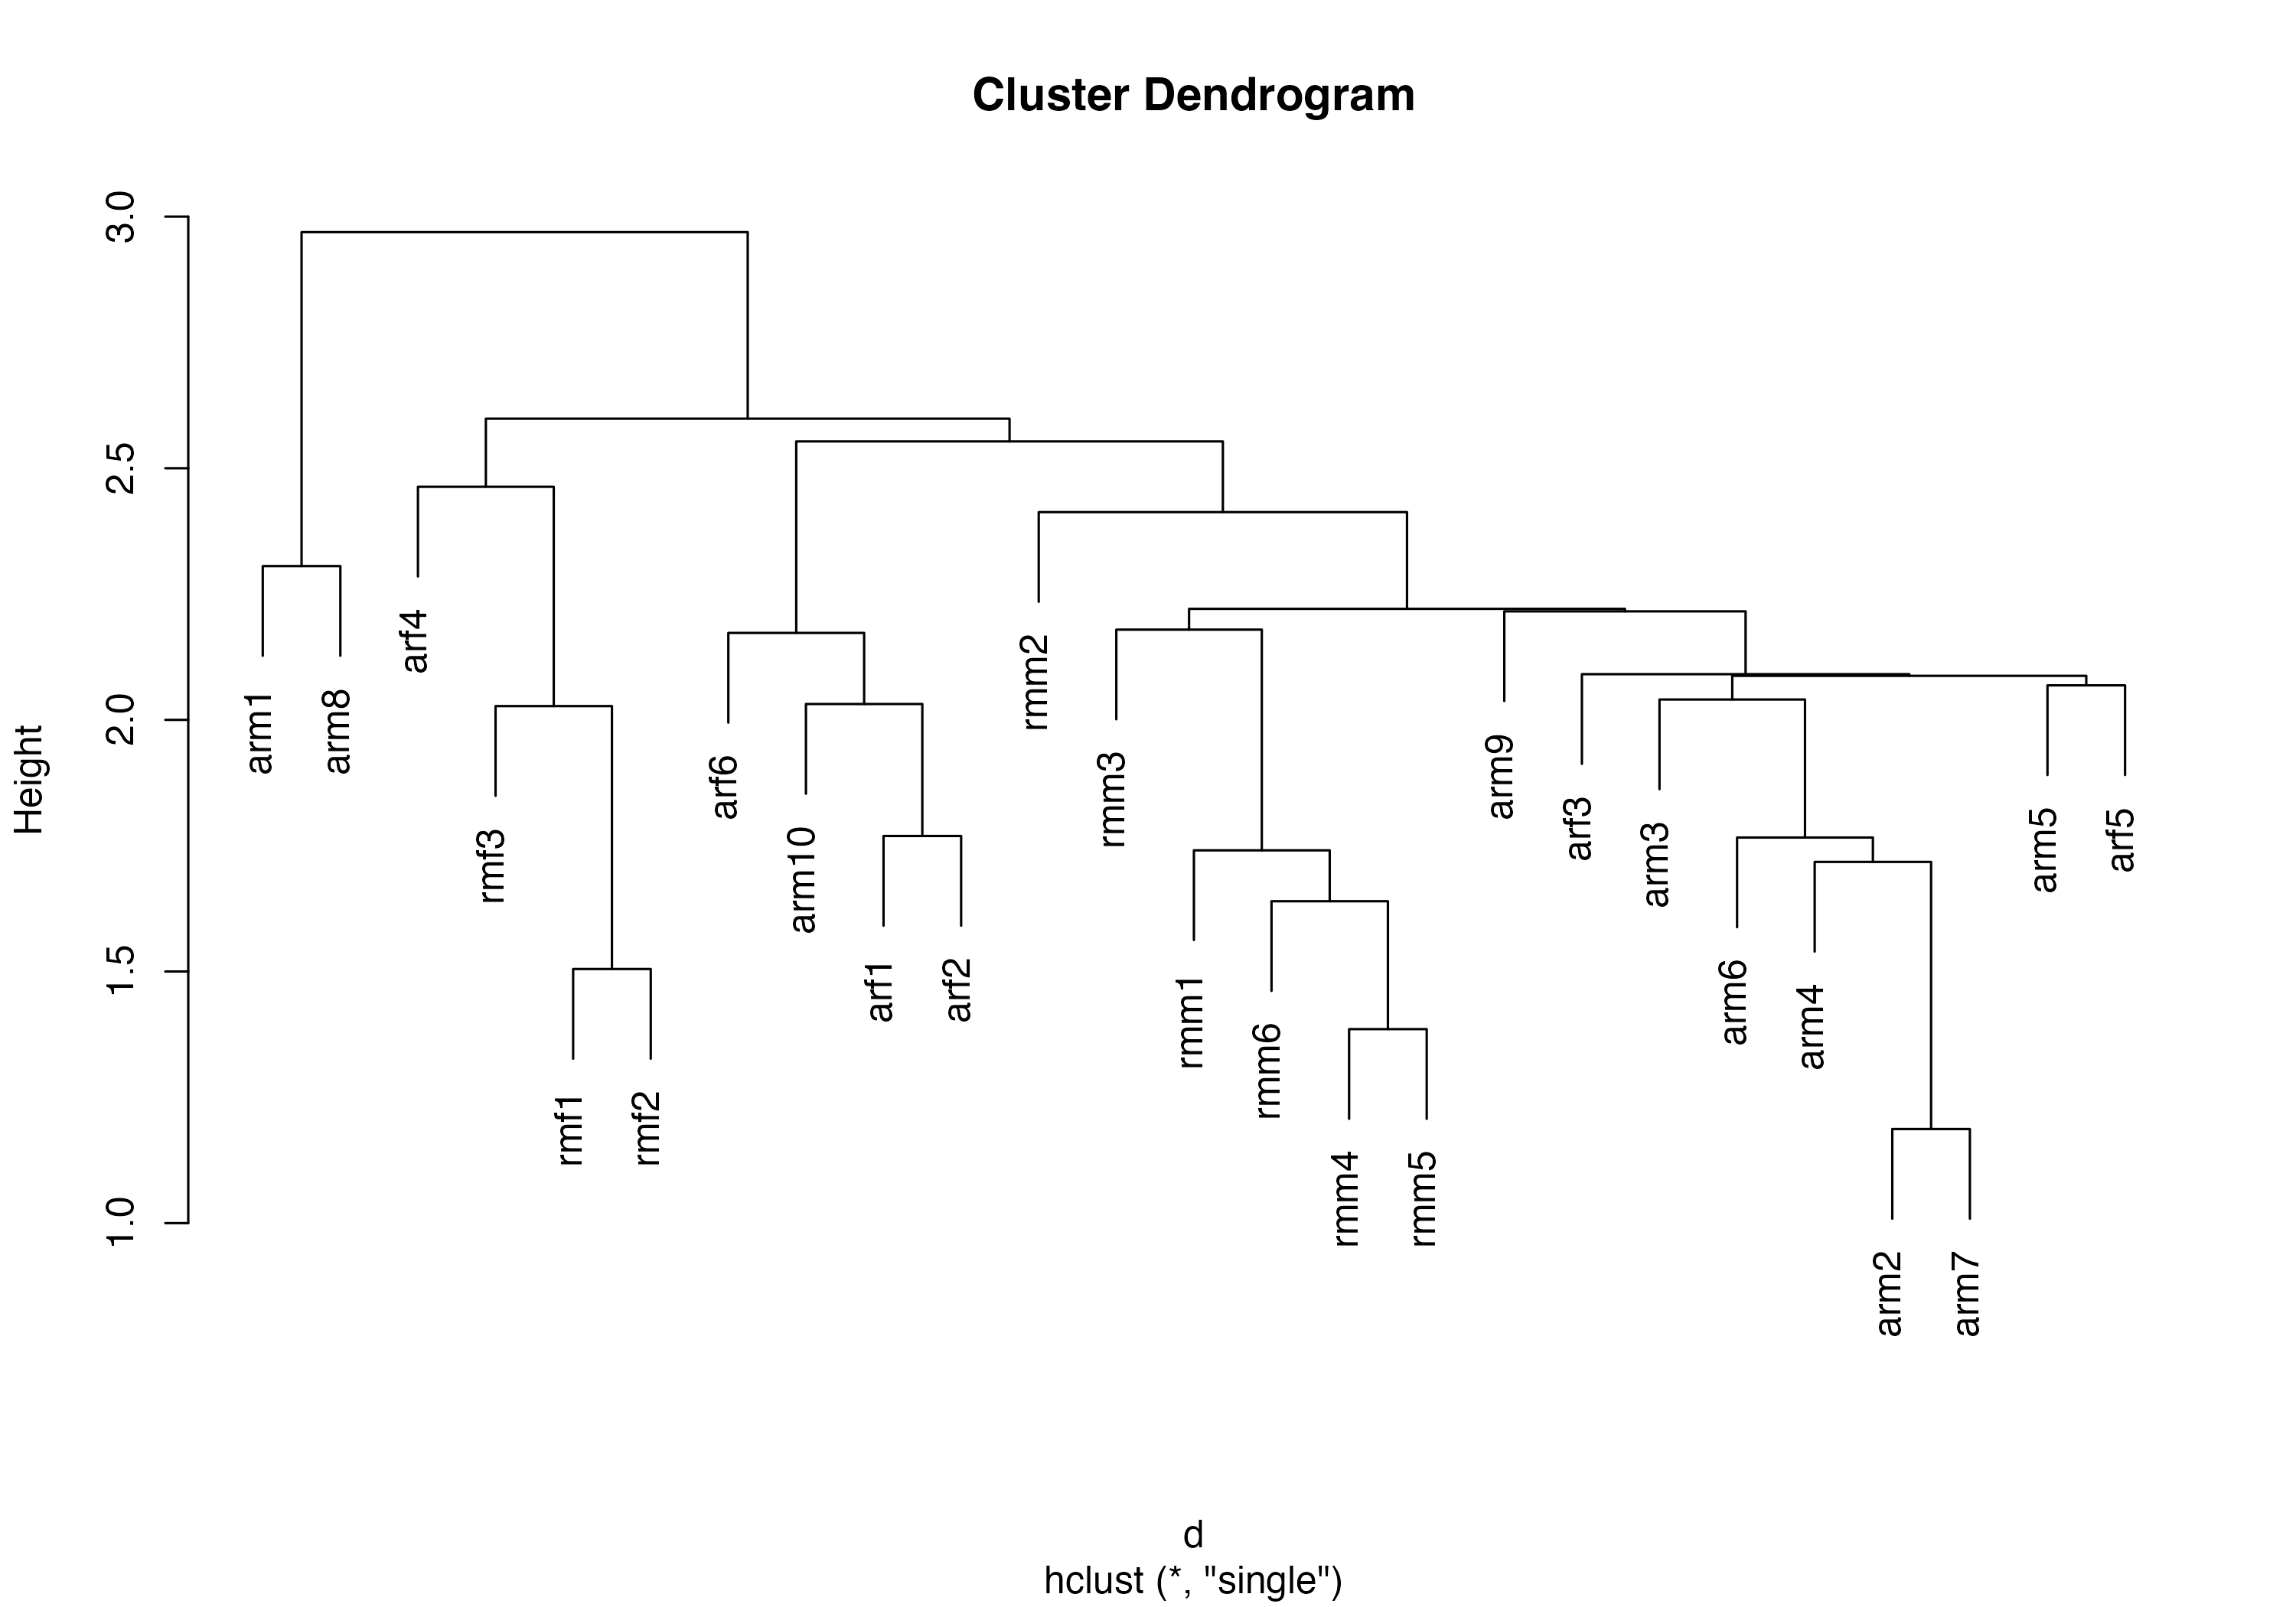
\includegraphics[keepaspectratio]{05_cluster_analysis_files/figure-beamer/fig-single-base-1.png}}

}

\caption{\label{fig-single-base}}

\end{figure}%
\end{frame}

\begin{frame}[fragile]{(1.1) Метод ближайшего соседа + \texttt{ape}}
\protect\phantomsection\label{ux43cux435ux442ux43eux434-ux431ux43bux438ux436ux430ux439ux448ux435ux433ux43e-ux441ux43eux441ux435ux434ux430-ape}
\begin{Shaded}
\begin{Highlighting}[]
\NormalTok{ph\_single }\OtherTok{\textless{}{-}} \FunctionTok{as.phylo}\NormalTok{(hc\_single)}
\FunctionTok{plot}\NormalTok{(ph\_single, }\AttributeTok{type =} \StringTok{"phylogram"}\NormalTok{)}
\FunctionTok{axisPhylo}\NormalTok{()}
\end{Highlighting}
\end{Shaded}

\begin{figure}[H]

\centering{

\pandocbounded{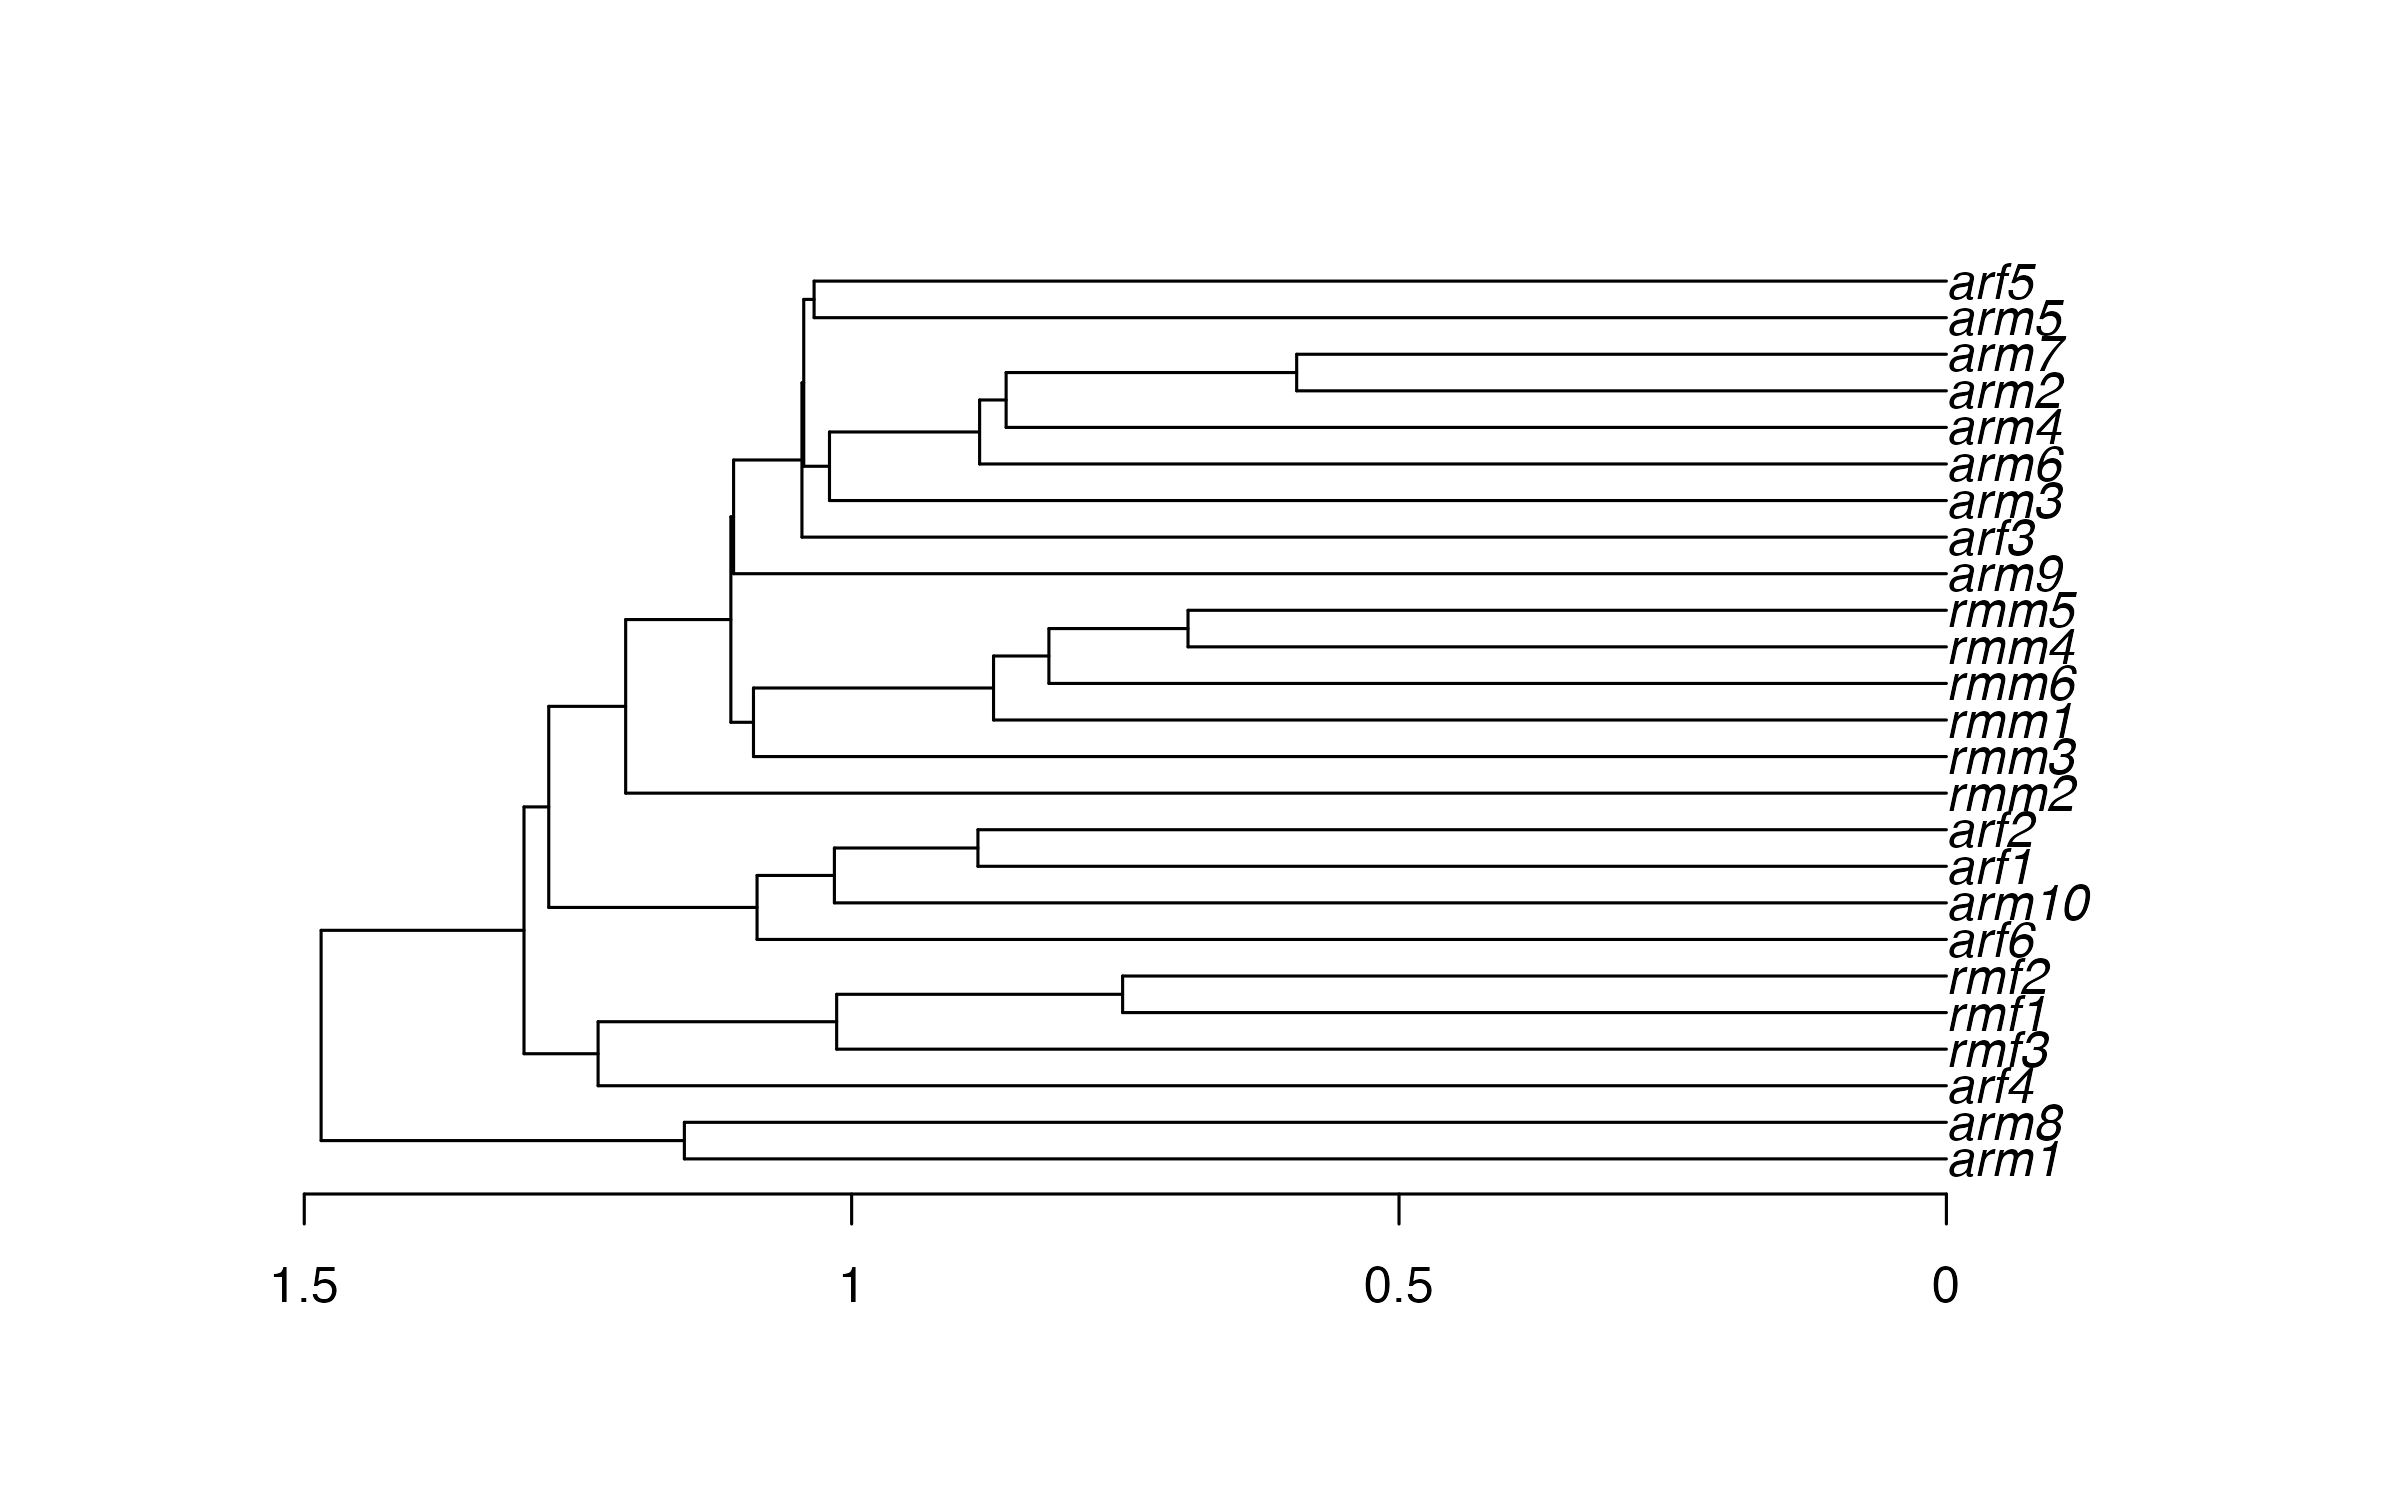
\includegraphics[keepaspectratio]{05_cluster_analysis_files/figure-beamer/fig-single-ape-1.png}}

}

\caption{\label{fig-single-ape}}

\end{figure}%
\end{frame}

\begin{frame}[fragile]{(1.2) Метод ближайшего соседа +
\texttt{dendextend}}
\protect\phantomsection\label{ux43cux435ux442ux43eux434-ux431ux43bux438ux436ux430ux439ux448ux435ux433ux43e-ux441ux43eux441ux435ux434ux430-dendextend}
\begin{Shaded}
\begin{Highlighting}[]
\NormalTok{den\_single }\OtherTok{\textless{}{-}} \FunctionTok{as.dendrogram}\NormalTok{(hc\_single)}
\FunctionTok{plot}\NormalTok{(den\_single, }\AttributeTok{horiz =} \ConstantTok{TRUE}\NormalTok{)}
\end{Highlighting}
\end{Shaded}

\begin{figure}[H]

\centering{

\pandocbounded{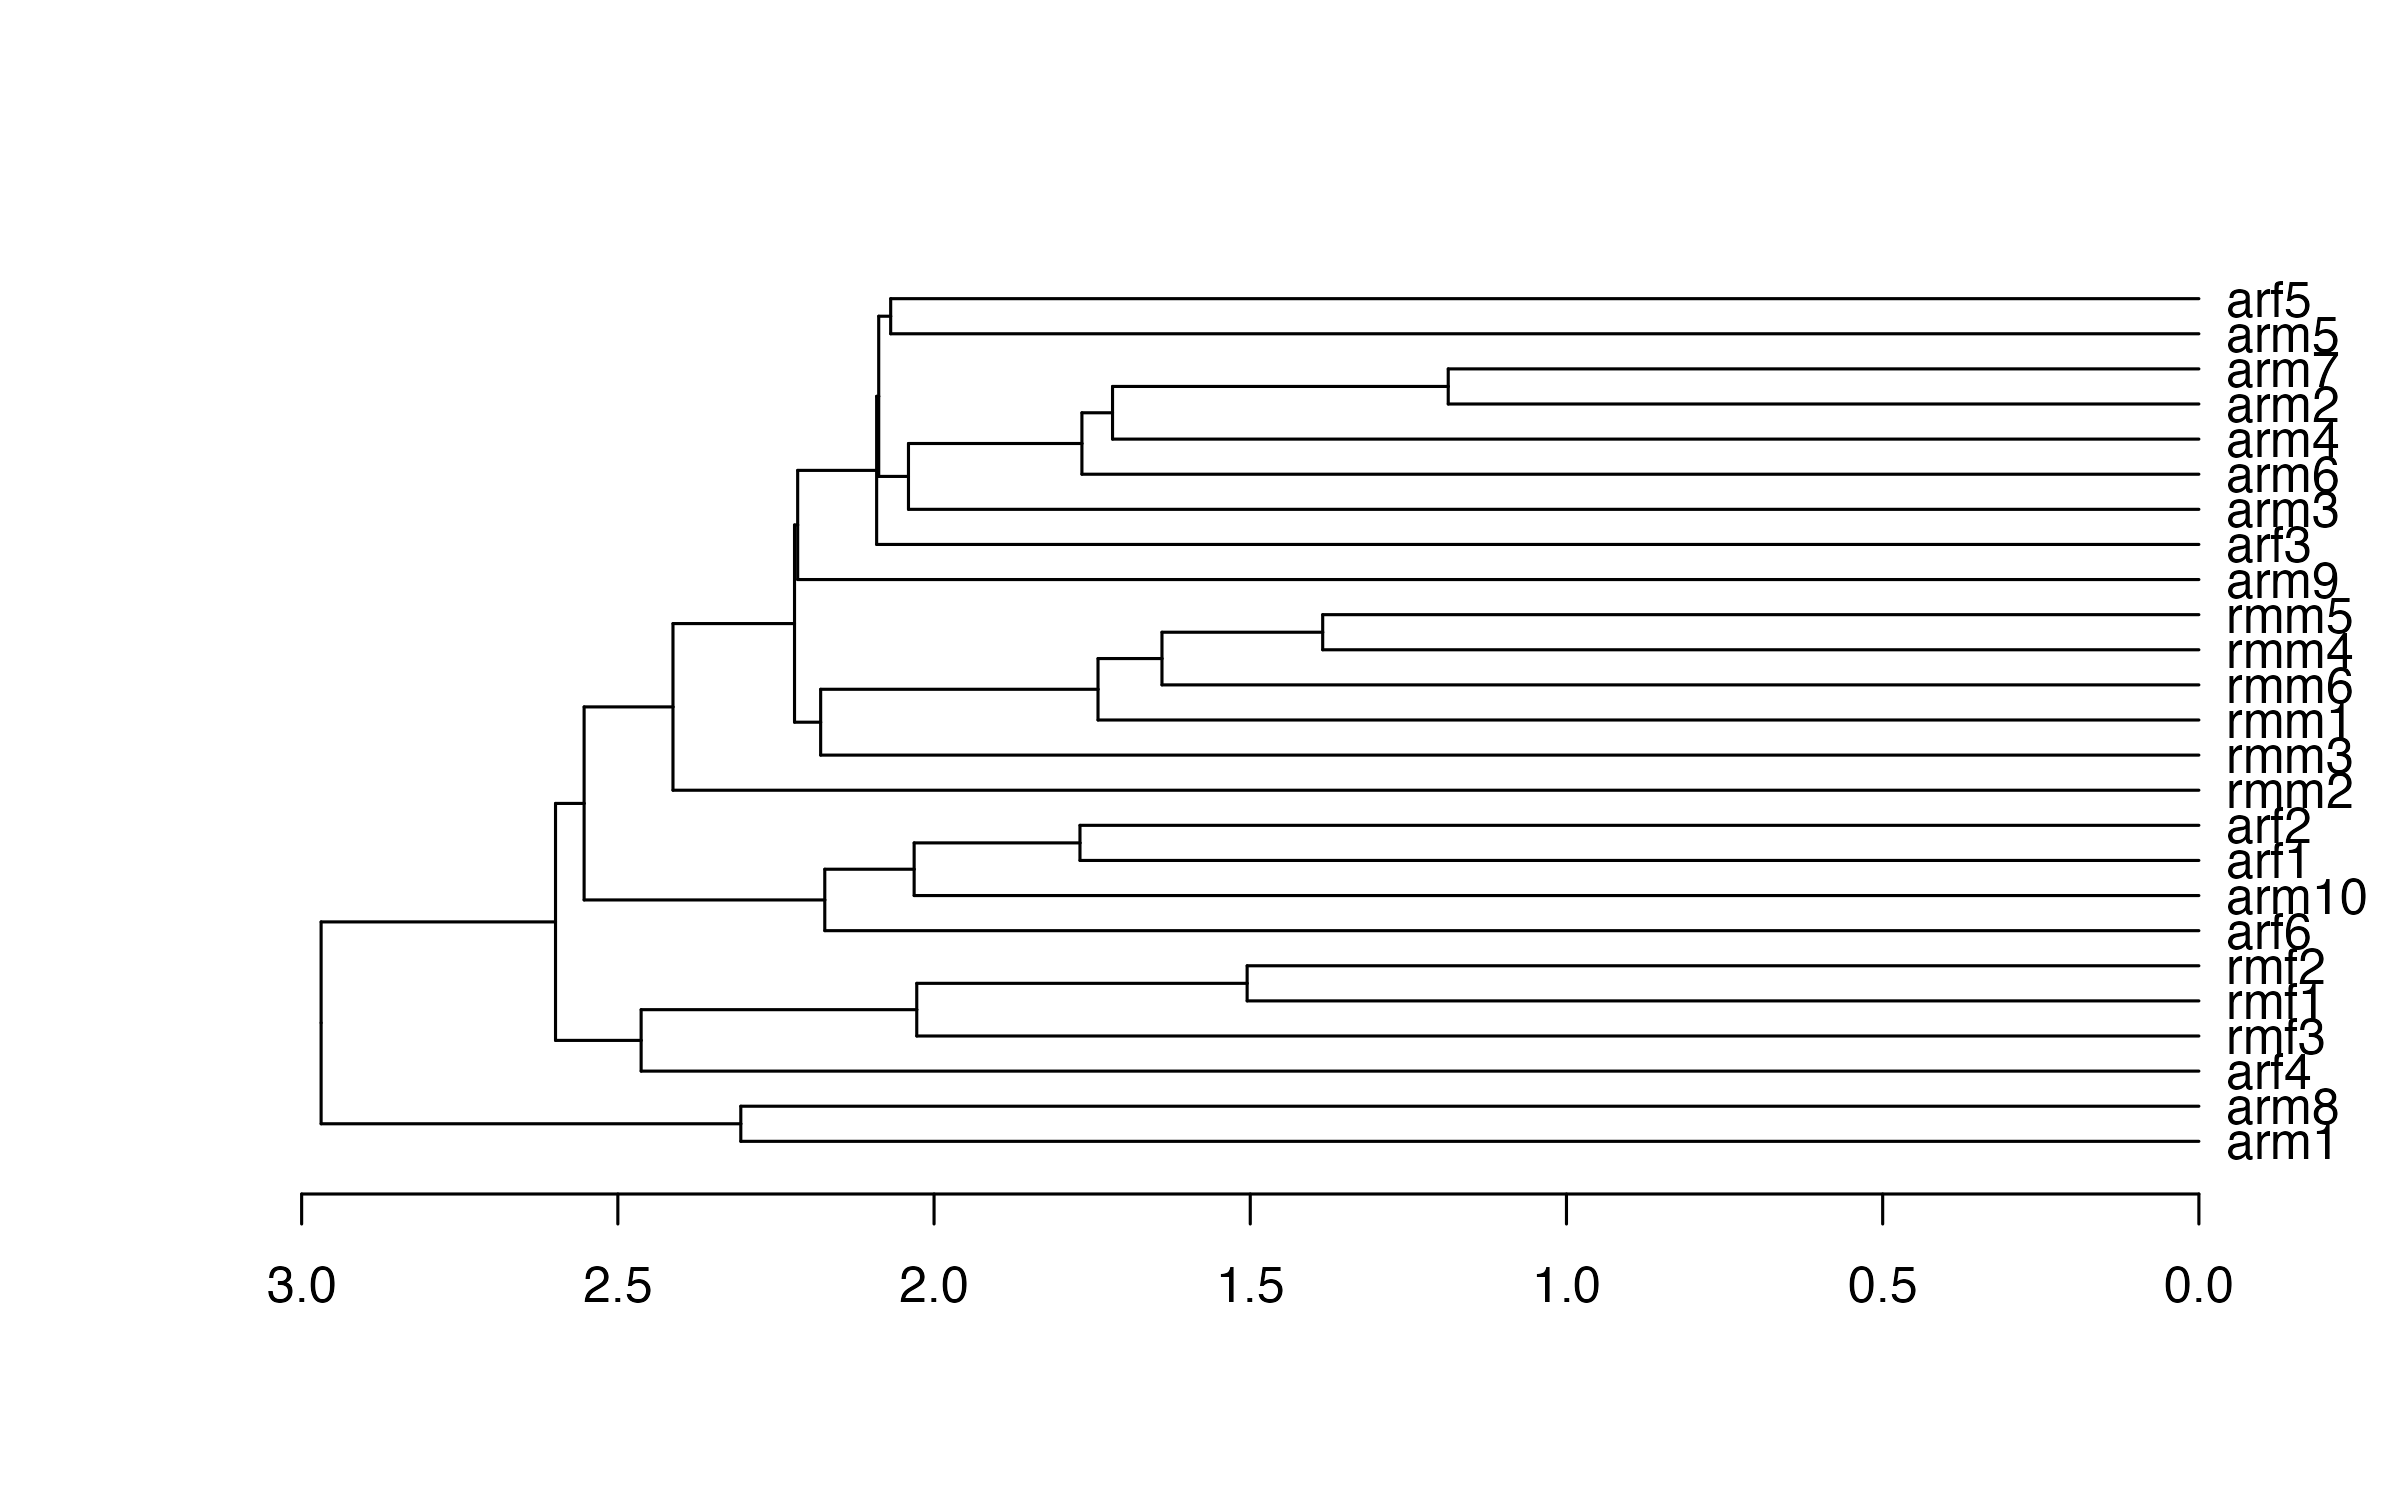
\includegraphics[keepaspectratio]{05_cluster_analysis_files/figure-beamer/fig-single-dend-1.png}}

}

\caption{\label{fig-single-dend}}

\end{figure}%
\end{frame}

\begin{frame}[fragile]{(2.1) Метод отдаленного соседа + \texttt{ape}}
\protect\phantomsection\label{ux43cux435ux442ux43eux434-ux43eux442ux434ux430ux43bux435ux43dux43dux43eux433ux43e-ux441ux43eux441ux435ux434ux430-ape}
\begin{Shaded}
\begin{Highlighting}[]
\NormalTok{hc\_compl }\OtherTok{\textless{}{-}} \FunctionTok{hclust}\NormalTok{(d, }\AttributeTok{method =} \StringTok{"complete"}\NormalTok{)}
\NormalTok{ph\_compl }\OtherTok{\textless{}{-}} \FunctionTok{as.phylo}\NormalTok{(hc\_compl)}
\FunctionTok{plot}\NormalTok{(ph\_compl, }\AttributeTok{type =} \StringTok{"phylogram"}\NormalTok{)}
\FunctionTok{axisPhylo}\NormalTok{()}
\end{Highlighting}
\end{Shaded}

\begin{figure}[H]

\centering{

\pandocbounded{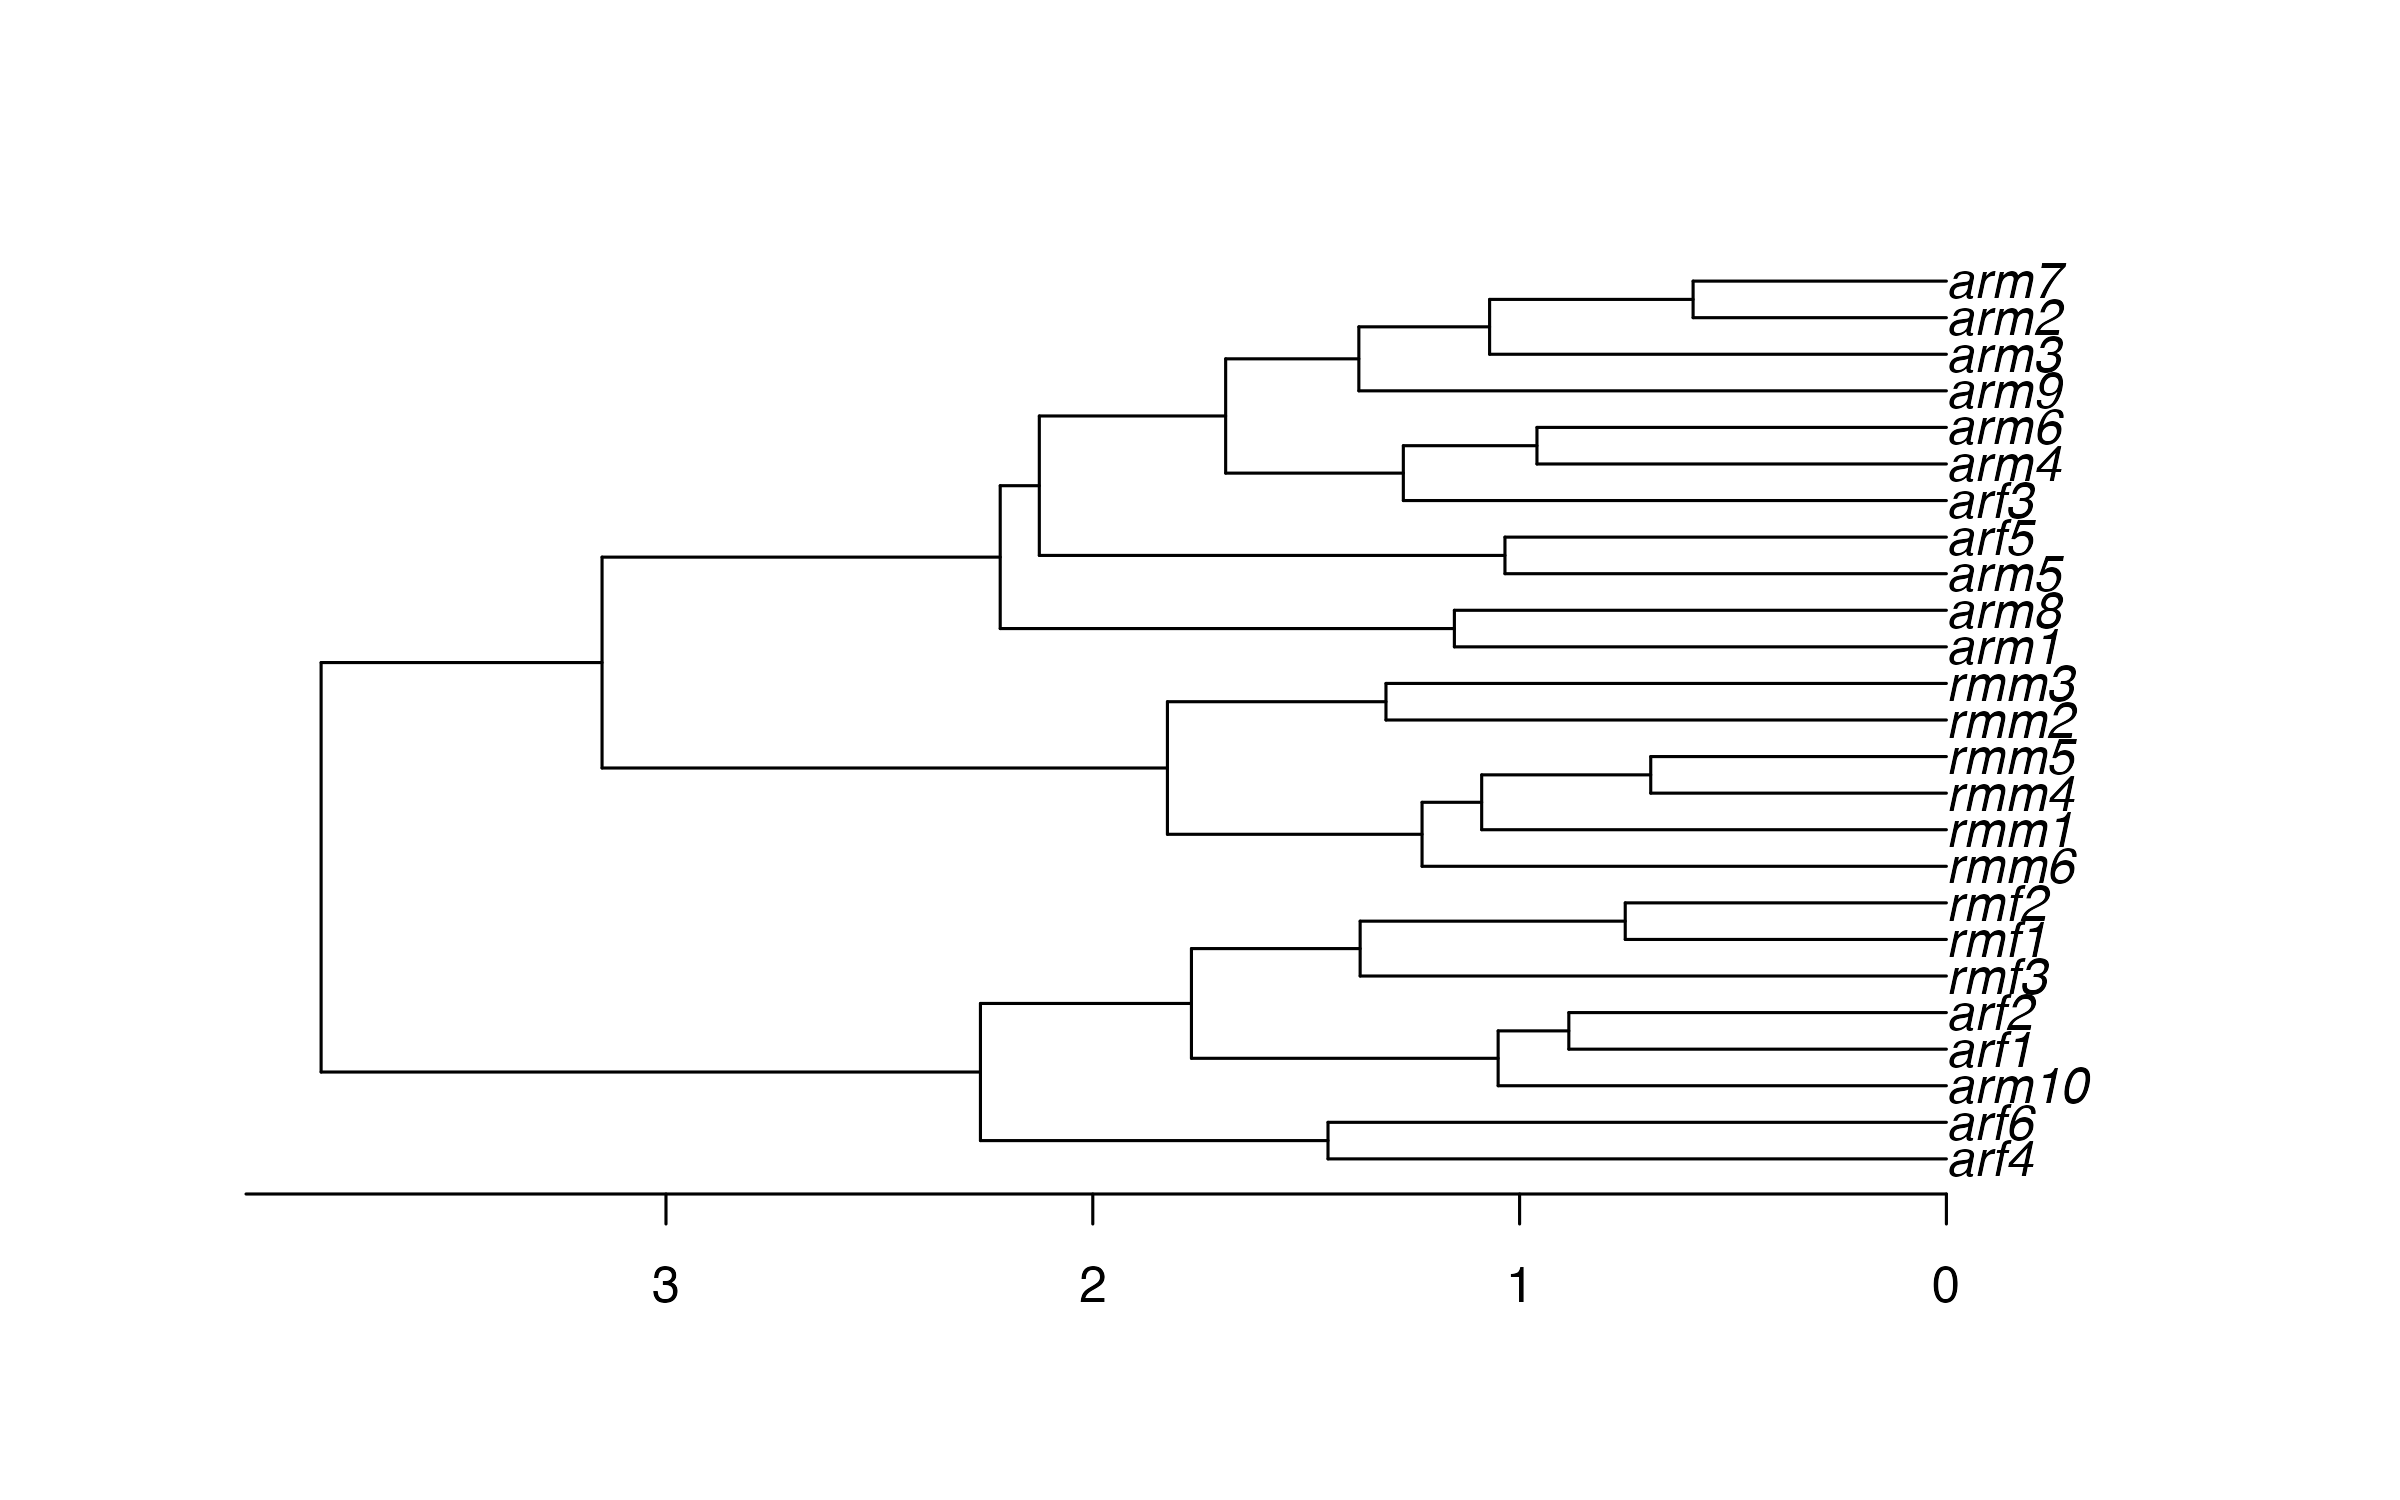
\includegraphics[keepaspectratio]{05_cluster_analysis_files/figure-beamer/fig-complete-ape-1.png}}

}

\caption{\label{fig-complete-ape}}

\end{figure}%
\end{frame}

\begin{frame}[fragile]{(2.2)Метод отдаленного соседа +
\texttt{dendextend}}
\protect\phantomsection\label{ux43cux435ux442ux43eux434-ux43eux442ux434ux430ux43bux435ux43dux43dux43eux433ux43e-ux441ux43eux441ux435ux434ux430-dendextend}
\begin{Shaded}
\begin{Highlighting}[]
\NormalTok{den\_compl }\OtherTok{\textless{}{-}} \FunctionTok{as.dendrogram}\NormalTok{(hc\_compl)}
\FunctionTok{plot}\NormalTok{(den\_compl, }\AttributeTok{horiz =} \ConstantTok{TRUE}\NormalTok{)}
\end{Highlighting}
\end{Shaded}

\begin{figure}[H]

\centering{

\pandocbounded{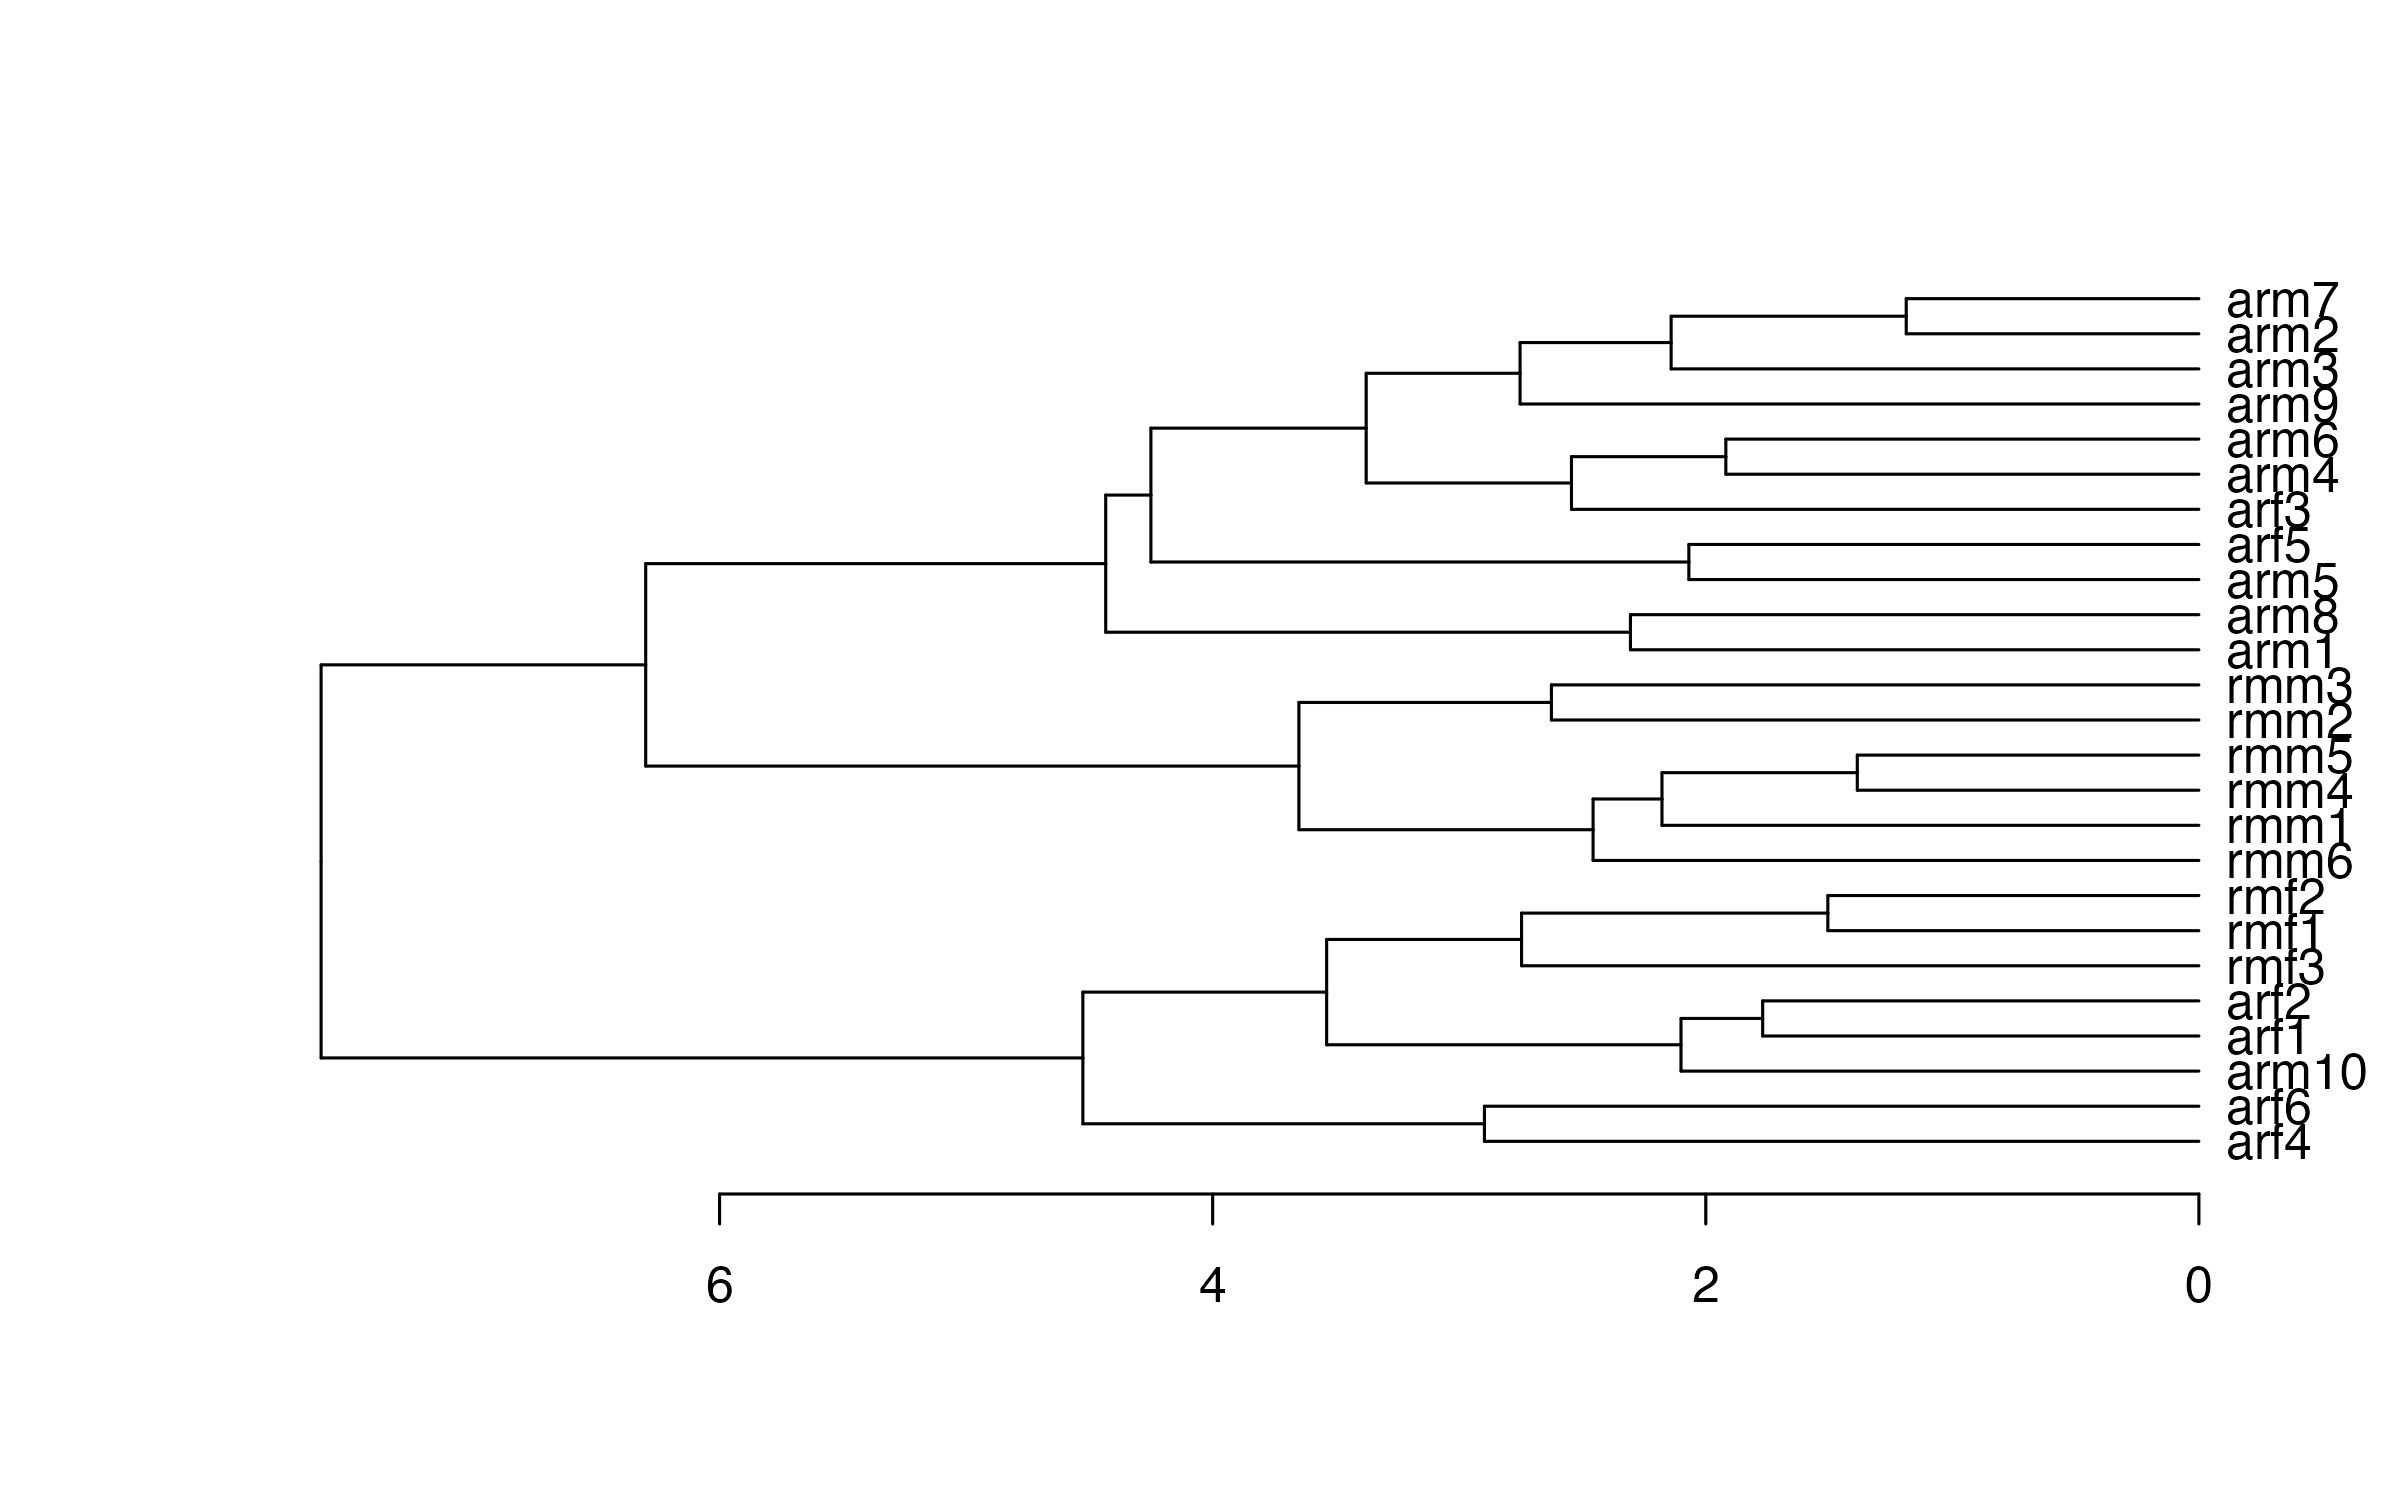
\includegraphics[keepaspectratio]{05_cluster_analysis_files/figure-beamer/fig-complete-dend-1.png}}

}

\caption{\label{fig-complete-dend}}

\end{figure}%
\end{frame}

\begin{frame}[fragile]{(3.1) Метод невзвешенного попарного среднего
(UPGMA) + \texttt{ape}}
\protect\phantomsection\label{ux43cux435ux442ux43eux434-ux43dux435ux432ux437ux432ux435ux448ux435ux43dux43dux43eux433ux43e-ux43fux43eux43fux430ux440ux43dux43eux433ux43e-ux441ux440ux435ux434ux43dux435ux433ux43e-upgma-ape}
\begin{Shaded}
\begin{Highlighting}[]
\NormalTok{hc\_avg }\OtherTok{\textless{}{-}} \FunctionTok{hclust}\NormalTok{(d, }\AttributeTok{method =} \StringTok{"average"}\NormalTok{)}
\NormalTok{ph\_avg }\OtherTok{\textless{}{-}} \FunctionTok{as.phylo}\NormalTok{(hc\_avg)}
\FunctionTok{plot}\NormalTok{(ph\_avg, }\AttributeTok{type =} \StringTok{"phylogram"}\NormalTok{)}
\FunctionTok{axisPhylo}\NormalTok{()}
\end{Highlighting}
\end{Shaded}

\begin{figure}[H]

\centering{

\pandocbounded{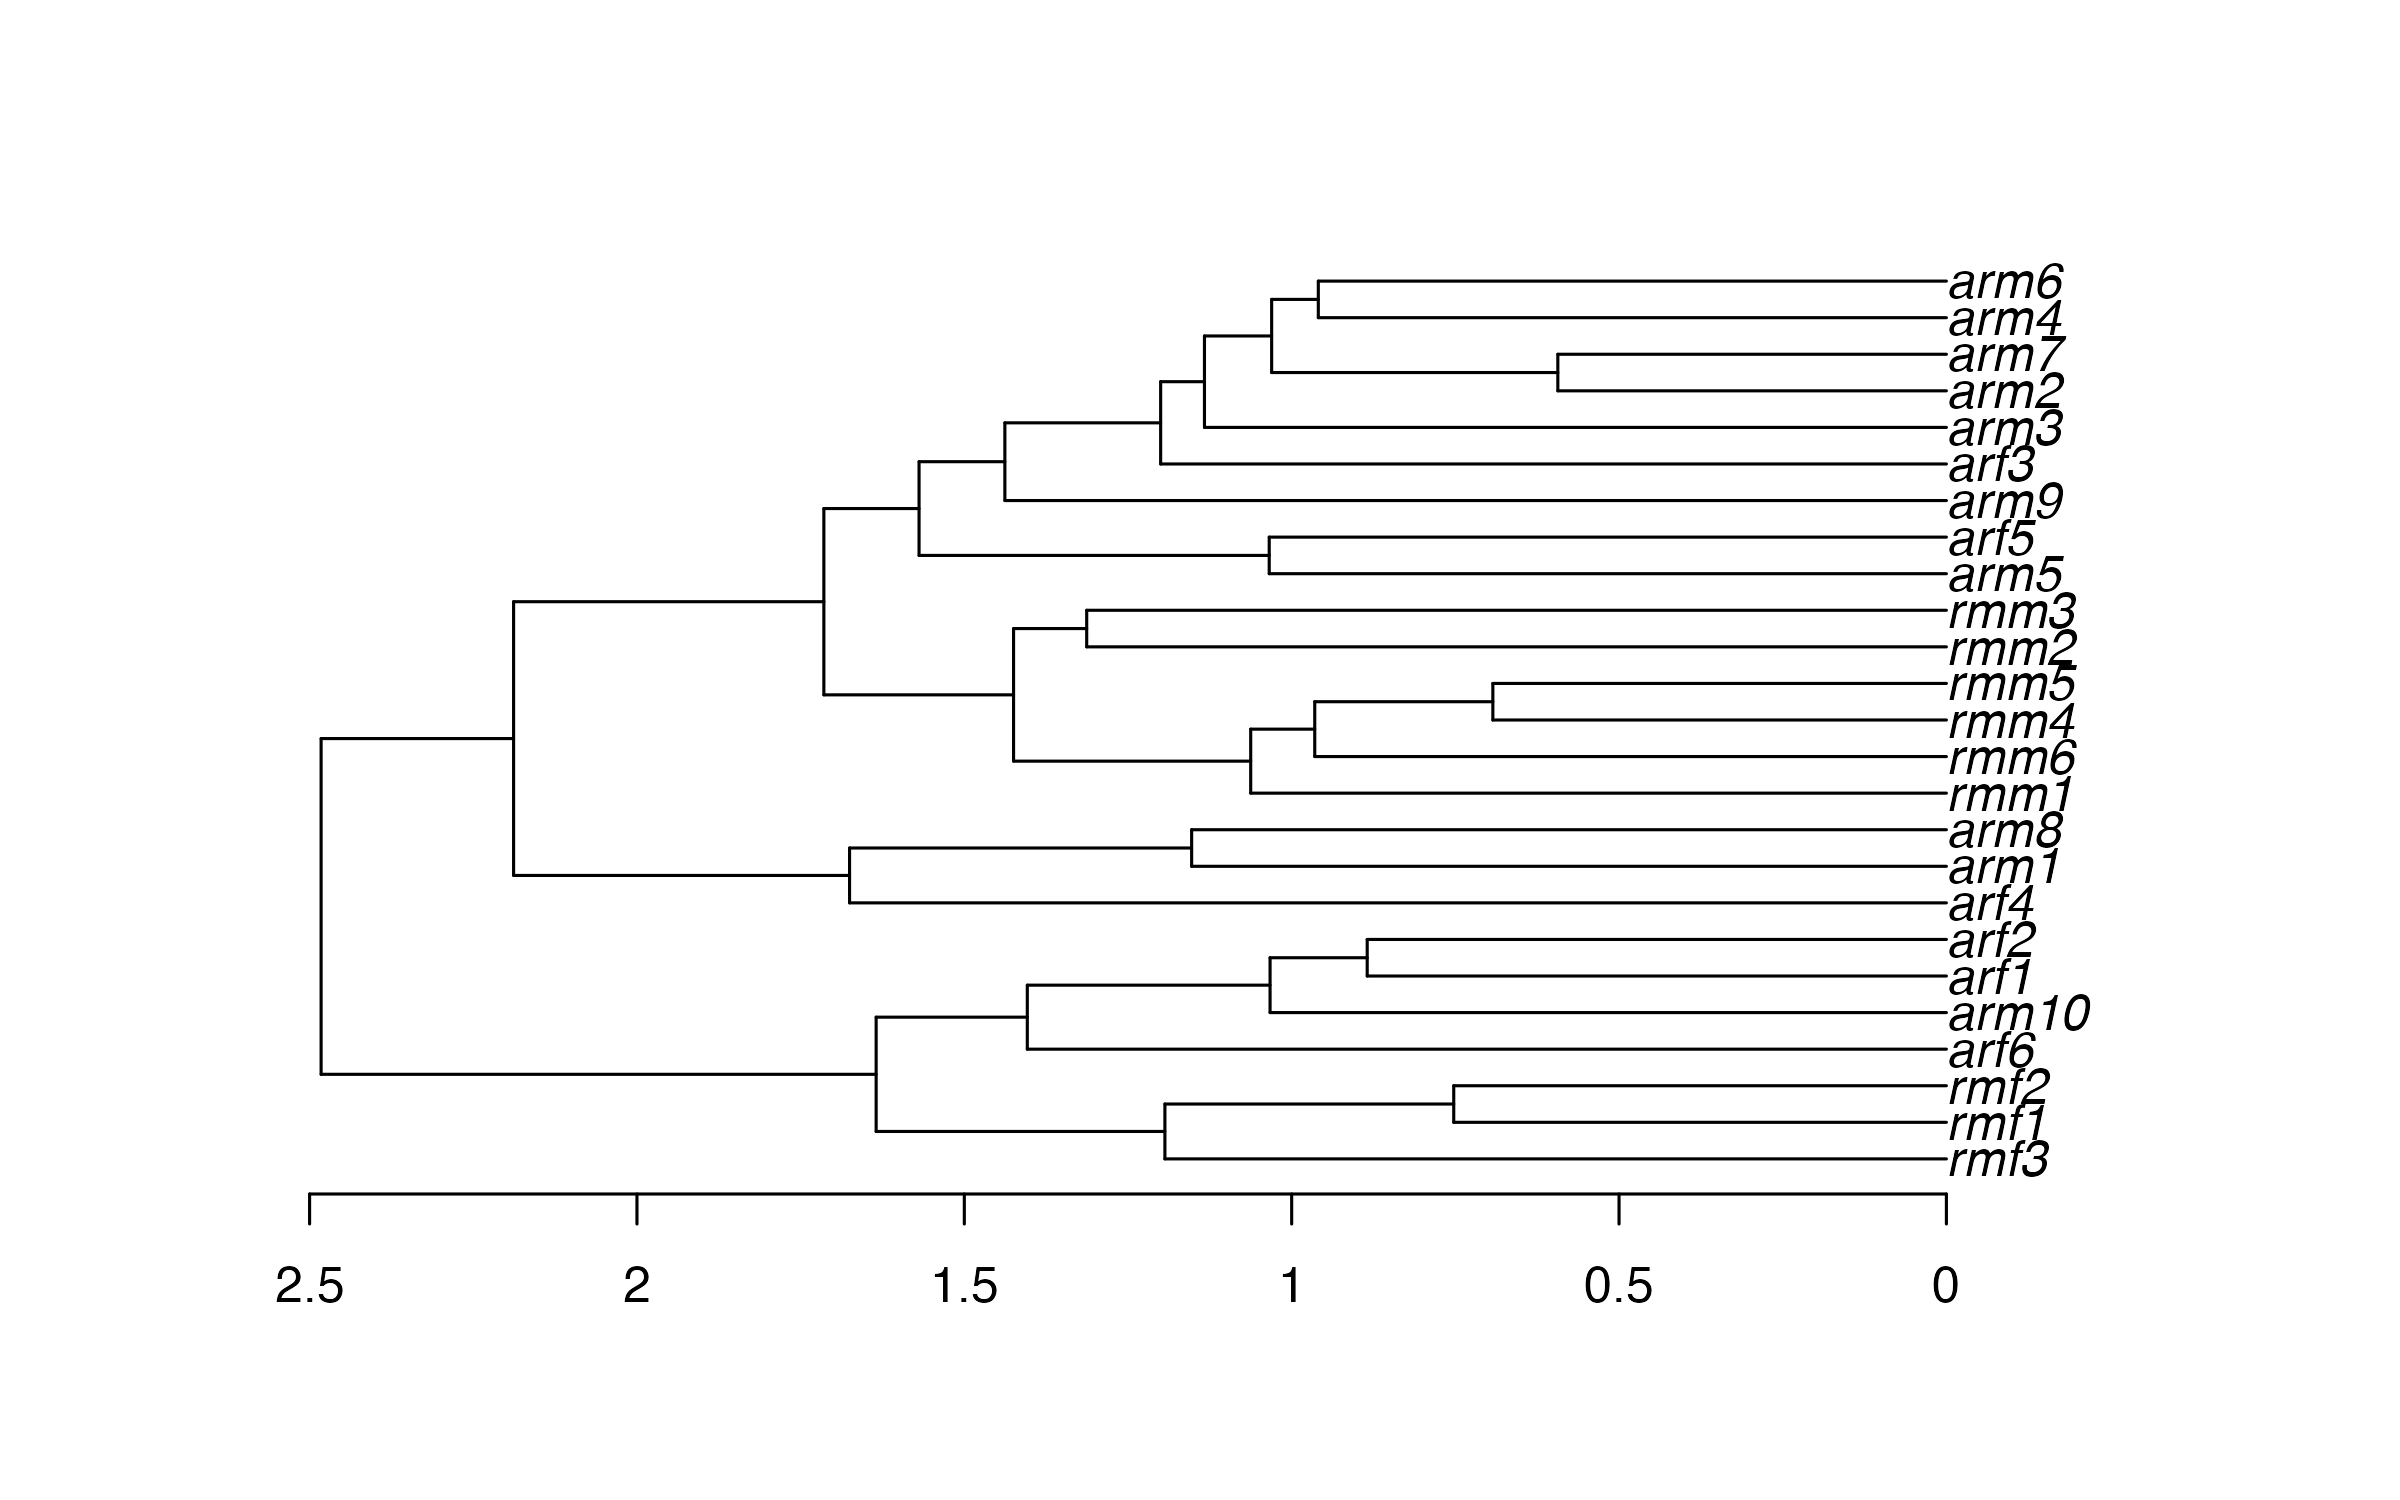
\includegraphics[keepaspectratio]{05_cluster_analysis_files/figure-beamer/fig-average-ape-1.png}}

}

\caption{\label{fig-average-ape}}

\end{figure}%
\end{frame}

\begin{frame}[fragile]{(3.2) Метод невзвешенного попарного среднего
(UPGMA) + \texttt{dendextend}}
\protect\phantomsection\label{ux43cux435ux442ux43eux434-ux43dux435ux432ux437ux432ux435ux448ux435ux43dux43dux43eux433ux43e-ux43fux43eux43fux430ux440ux43dux43eux433ux43e-ux441ux440ux435ux434ux43dux435ux433ux43e-upgma-dendextend}
\begin{Shaded}
\begin{Highlighting}[]
\NormalTok{den\_avg }\OtherTok{\textless{}{-}} \FunctionTok{as.dendrogram}\NormalTok{(hc\_avg)}
\FunctionTok{plot}\NormalTok{(den\_avg, }\AttributeTok{horiz =} \ConstantTok{TRUE}\NormalTok{)}
\end{Highlighting}
\end{Shaded}

\begin{figure}[H]

\centering{

\pandocbounded{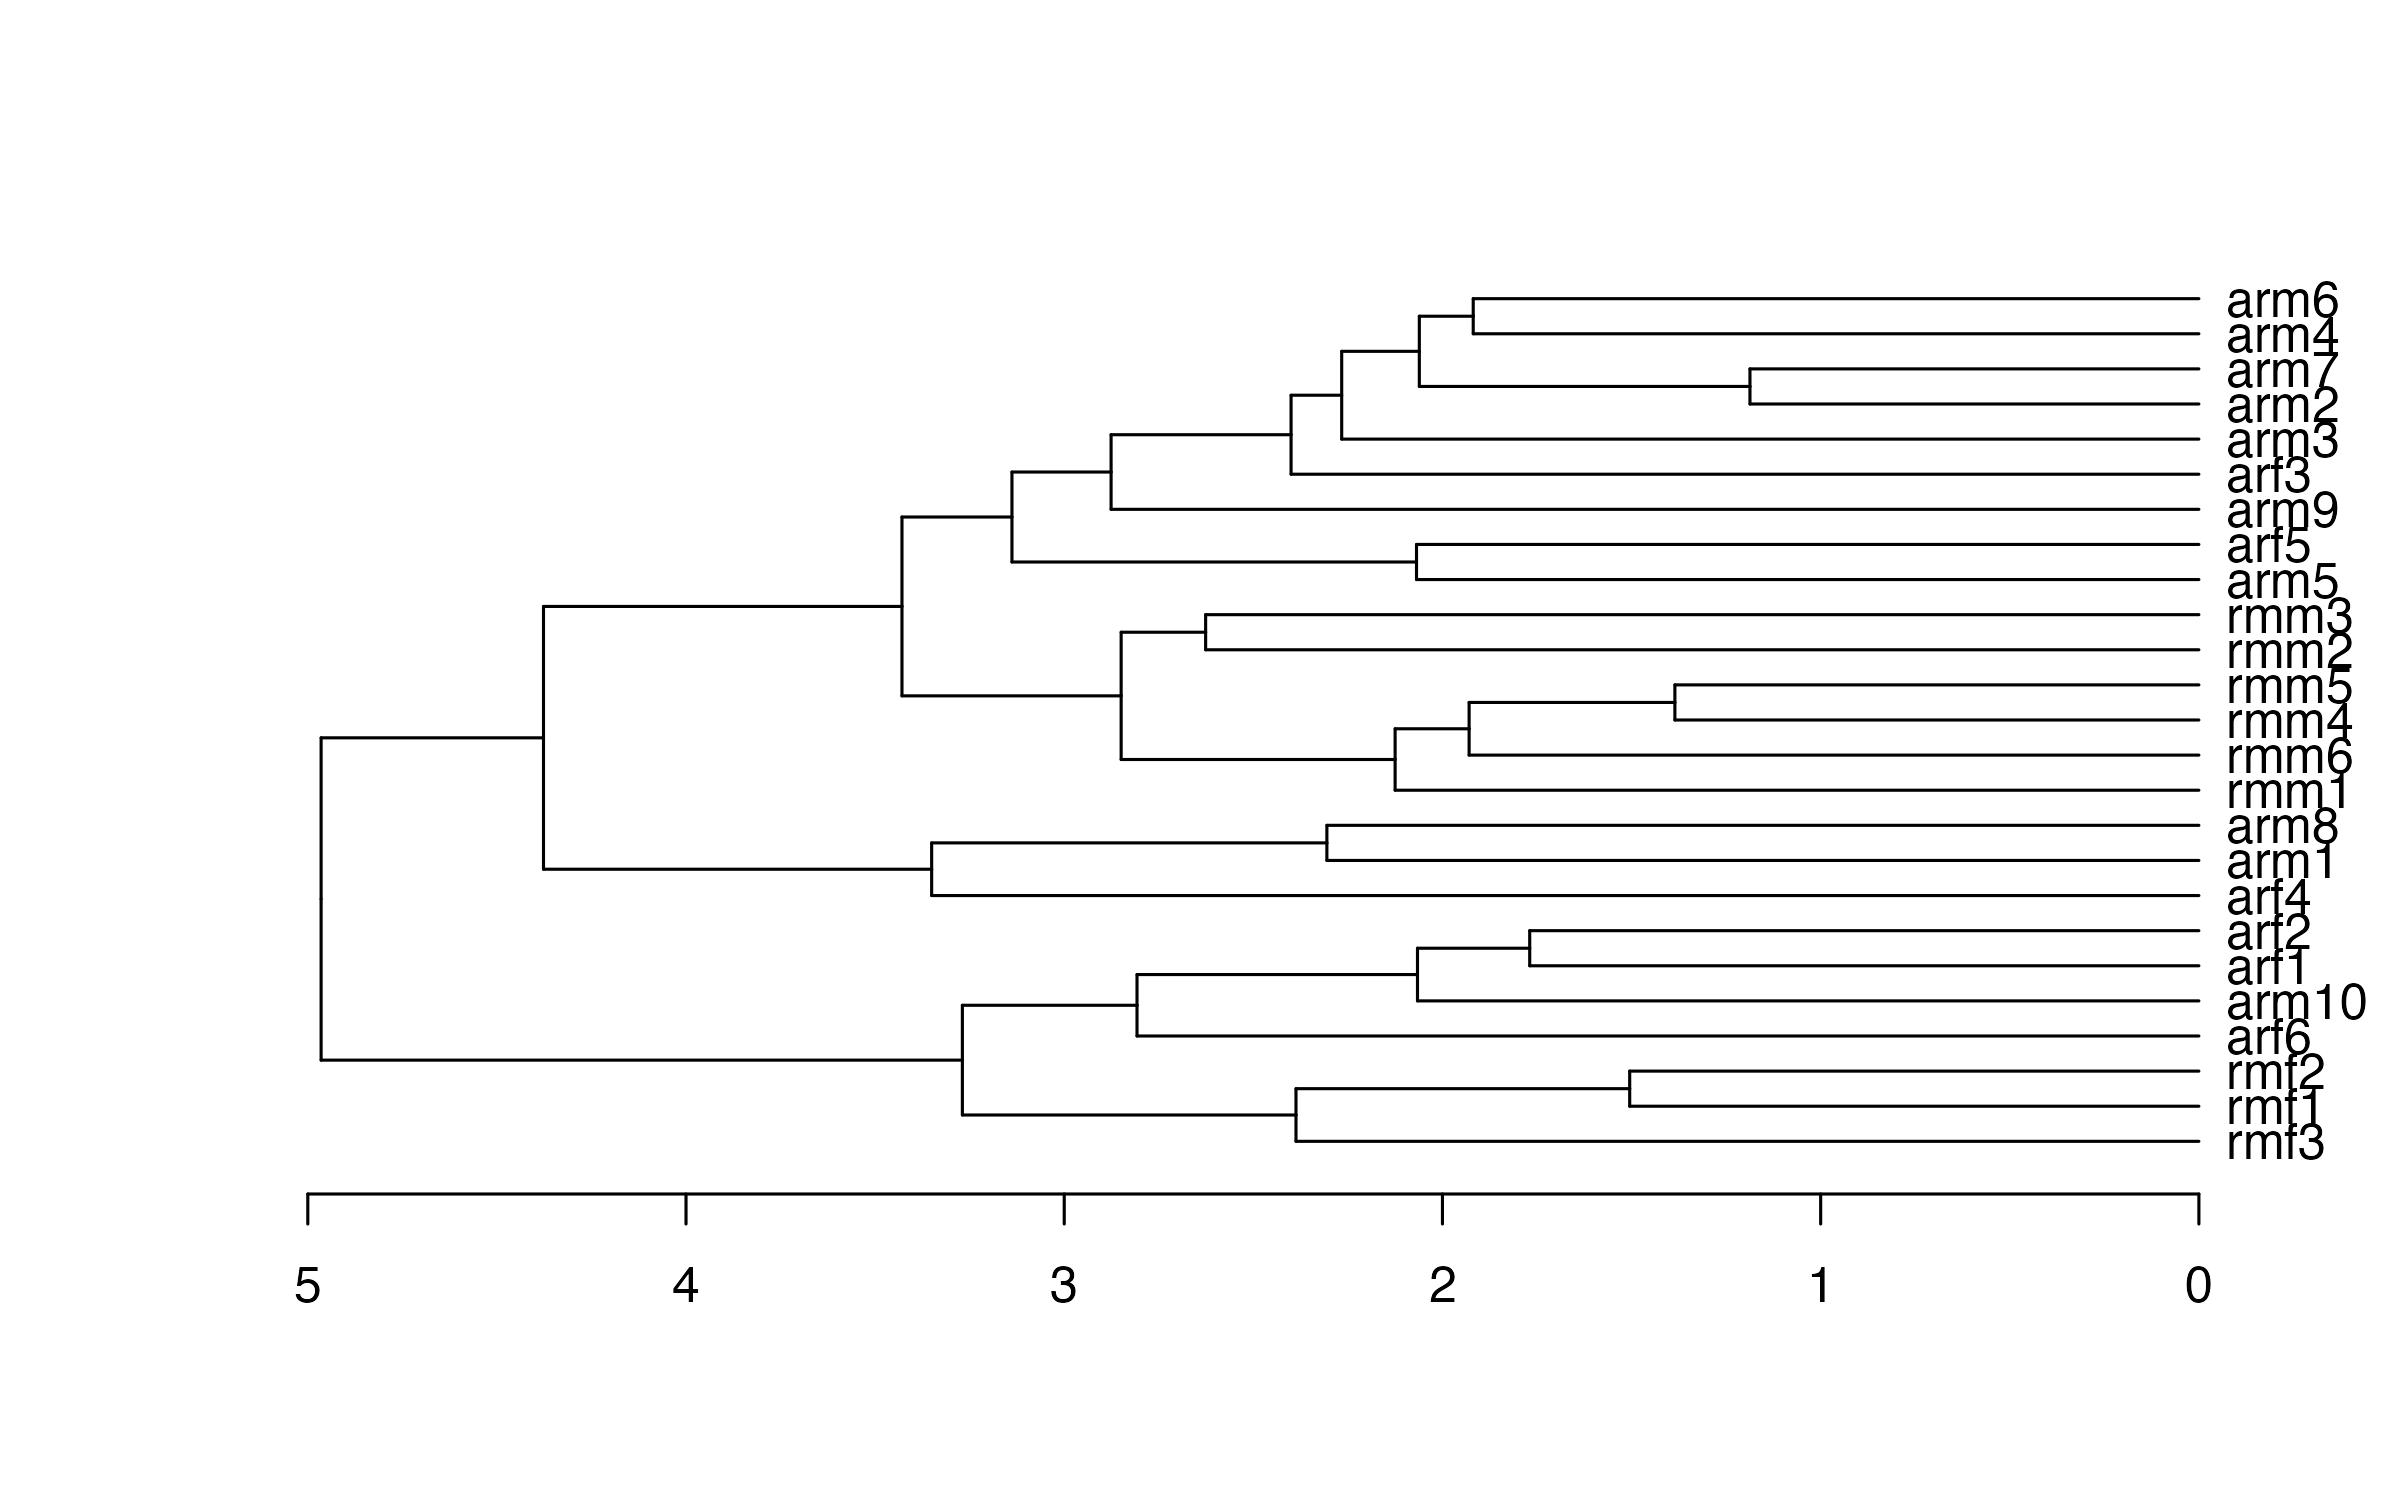
\includegraphics[keepaspectratio]{05_cluster_analysis_files/figure-beamer/fig-average-dend-1.png}}

}

\caption{\label{fig-average-dend}}

\end{figure}%
\end{frame}

\begin{frame}[fragile]{(4.1) Метод Варда + \texttt{ape}}
\protect\phantomsection\label{ux43cux435ux442ux43eux434-ux432ux430ux440ux434ux430-ape}
\begin{Shaded}
\begin{Highlighting}[]
\NormalTok{hc\_w2 }\OtherTok{\textless{}{-}}\FunctionTok{hclust}\NormalTok{(d, }\AttributeTok{method =} \StringTok{"ward.D2"}\NormalTok{)}
\NormalTok{ph\_w2 }\OtherTok{\textless{}{-}} \FunctionTok{as.phylo}\NormalTok{(hc\_w2)}
\FunctionTok{plot}\NormalTok{(ph\_w2, }\AttributeTok{type =} \StringTok{"phylogram"}\NormalTok{)}
\FunctionTok{axisPhylo}\NormalTok{()}
\end{Highlighting}
\end{Shaded}

\begin{figure}[H]

\centering{

\pandocbounded{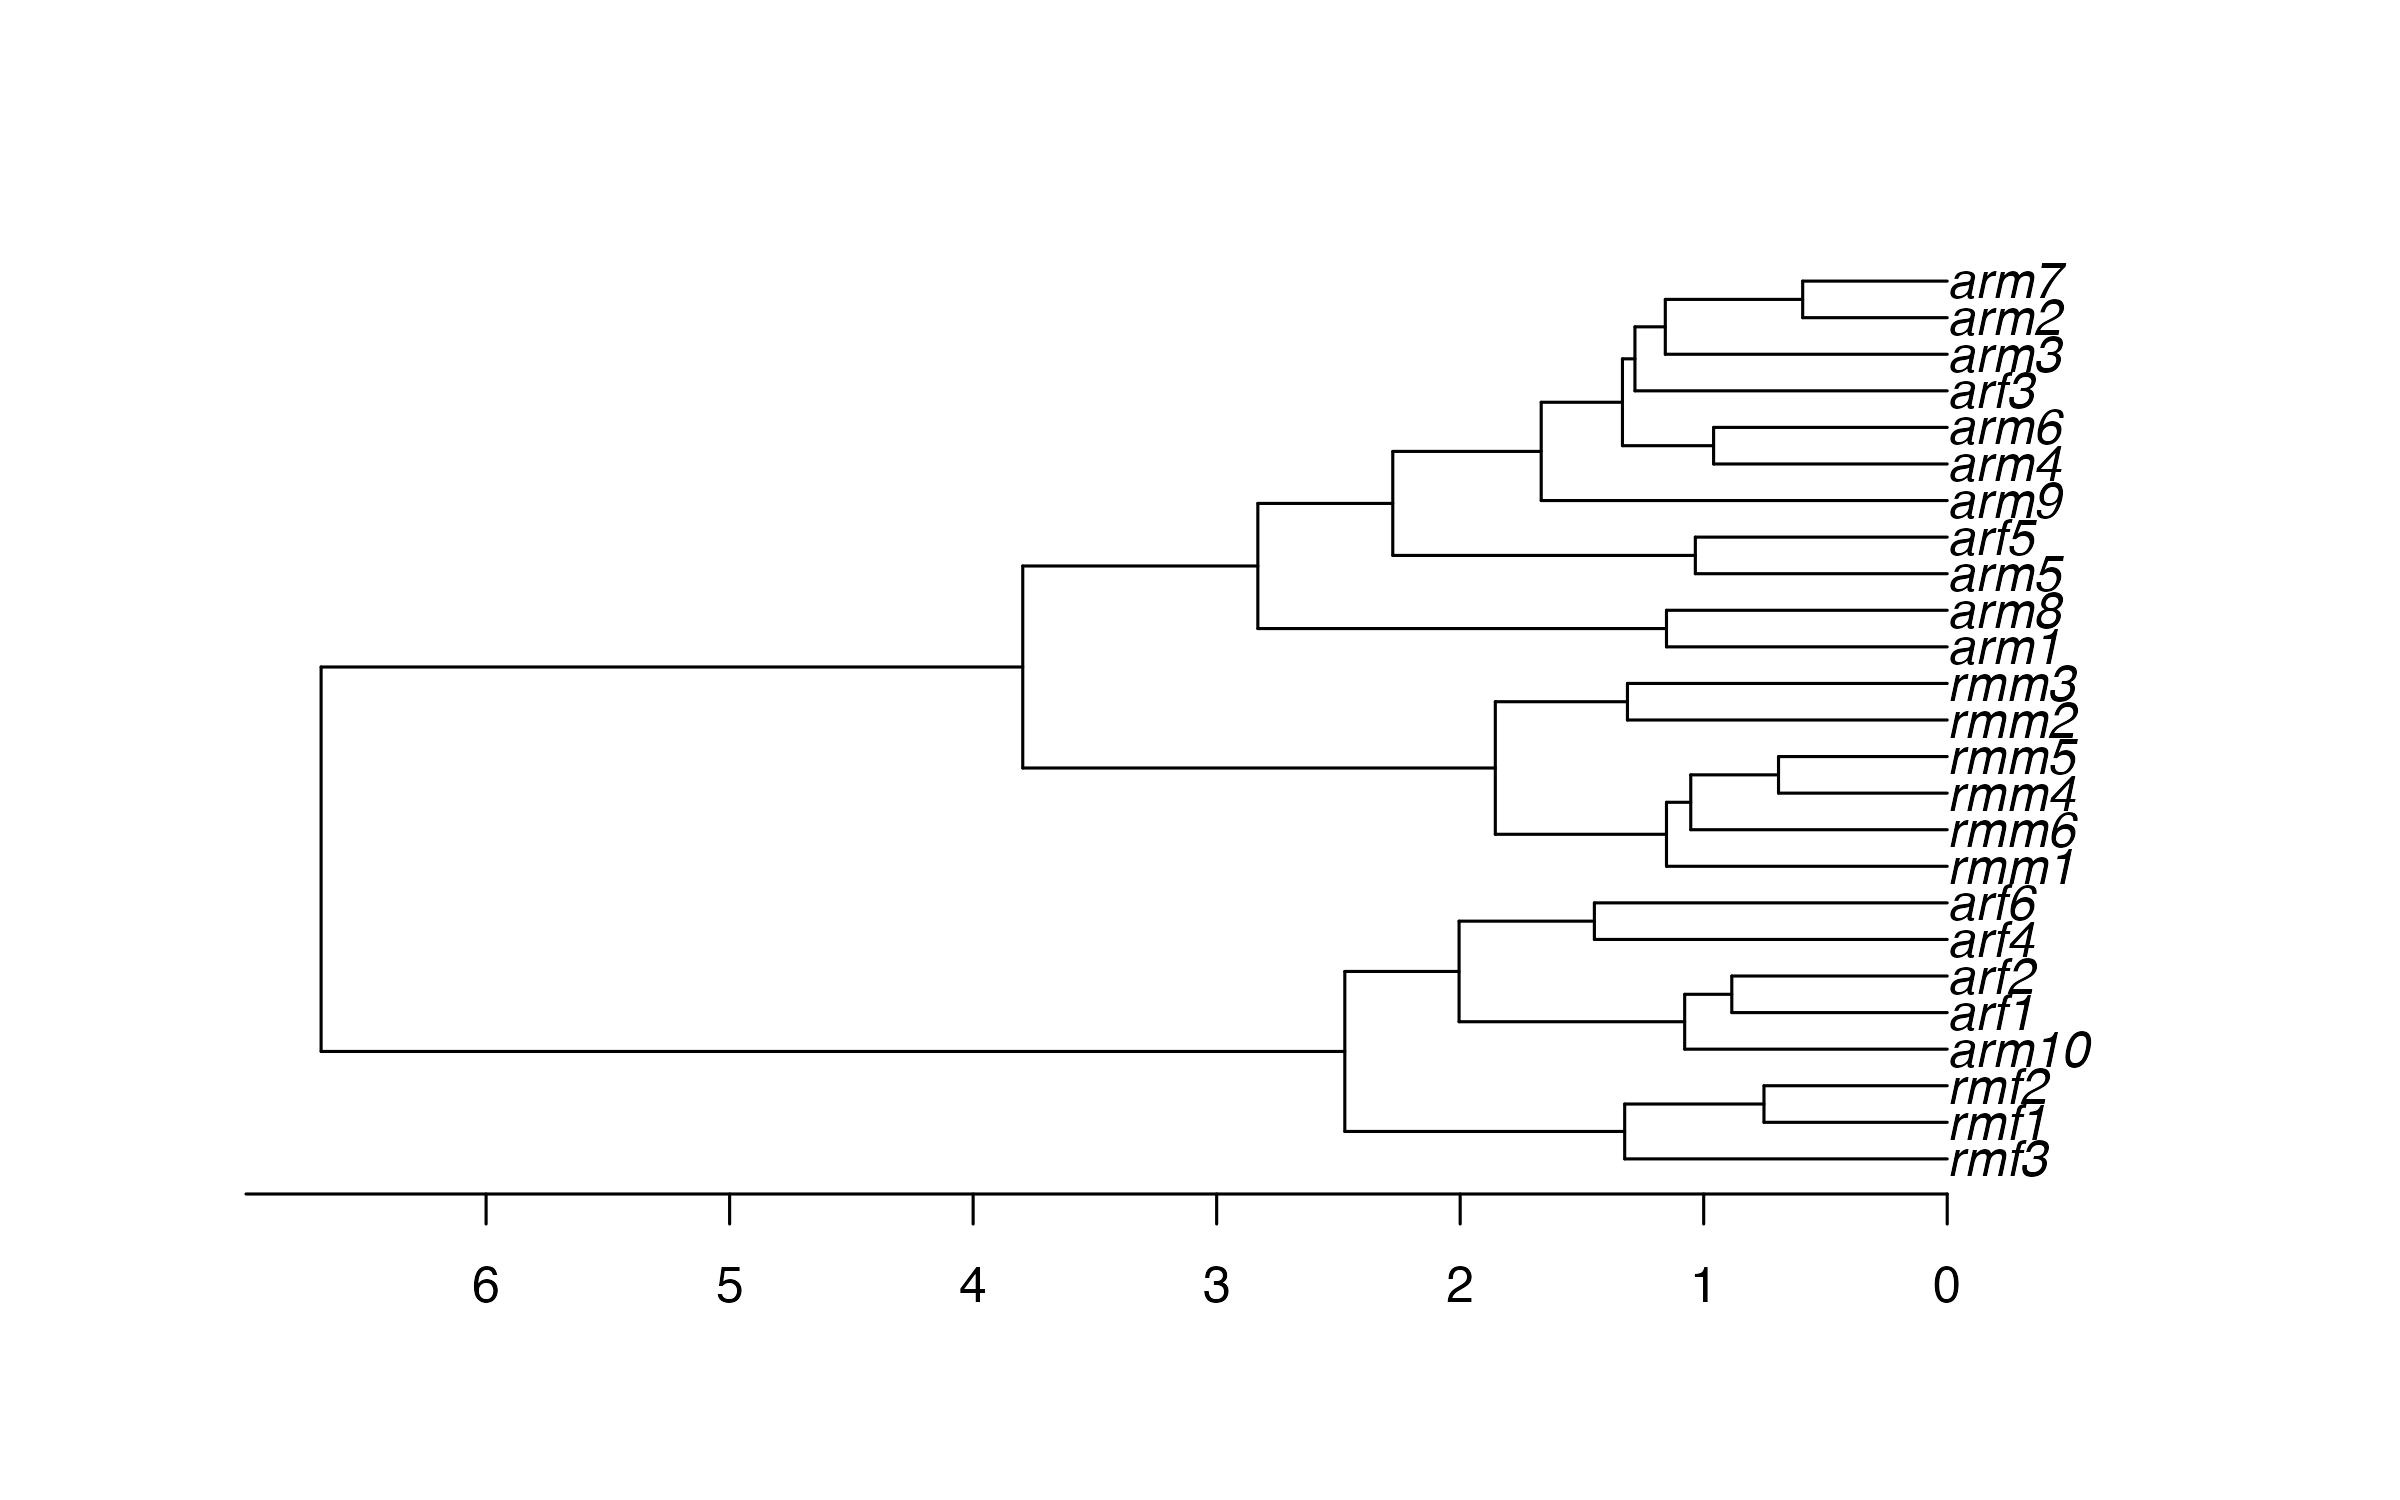
\includegraphics[keepaspectratio]{05_cluster_analysis_files/figure-beamer/fig-ward-ape-1.png}}

}

\caption{\label{fig-ward-ape}}

\end{figure}%
\end{frame}

\begin{frame}[fragile]{(4.2) Метод Варда + \texttt{dendextend}}
\protect\phantomsection\label{ux43cux435ux442ux43eux434-ux432ux430ux440ux434ux430-dendextend}
\begin{Shaded}
\begin{Highlighting}[]
\NormalTok{den\_w2 }\OtherTok{\textless{}{-}} \FunctionTok{as.dendrogram}\NormalTok{(hc\_w2)}
\FunctionTok{plot}\NormalTok{(den\_w2, }\AttributeTok{horiz =} \ConstantTok{TRUE}\NormalTok{)}
\end{Highlighting}
\end{Shaded}

\begin{figure}[H]

\centering{

\pandocbounded{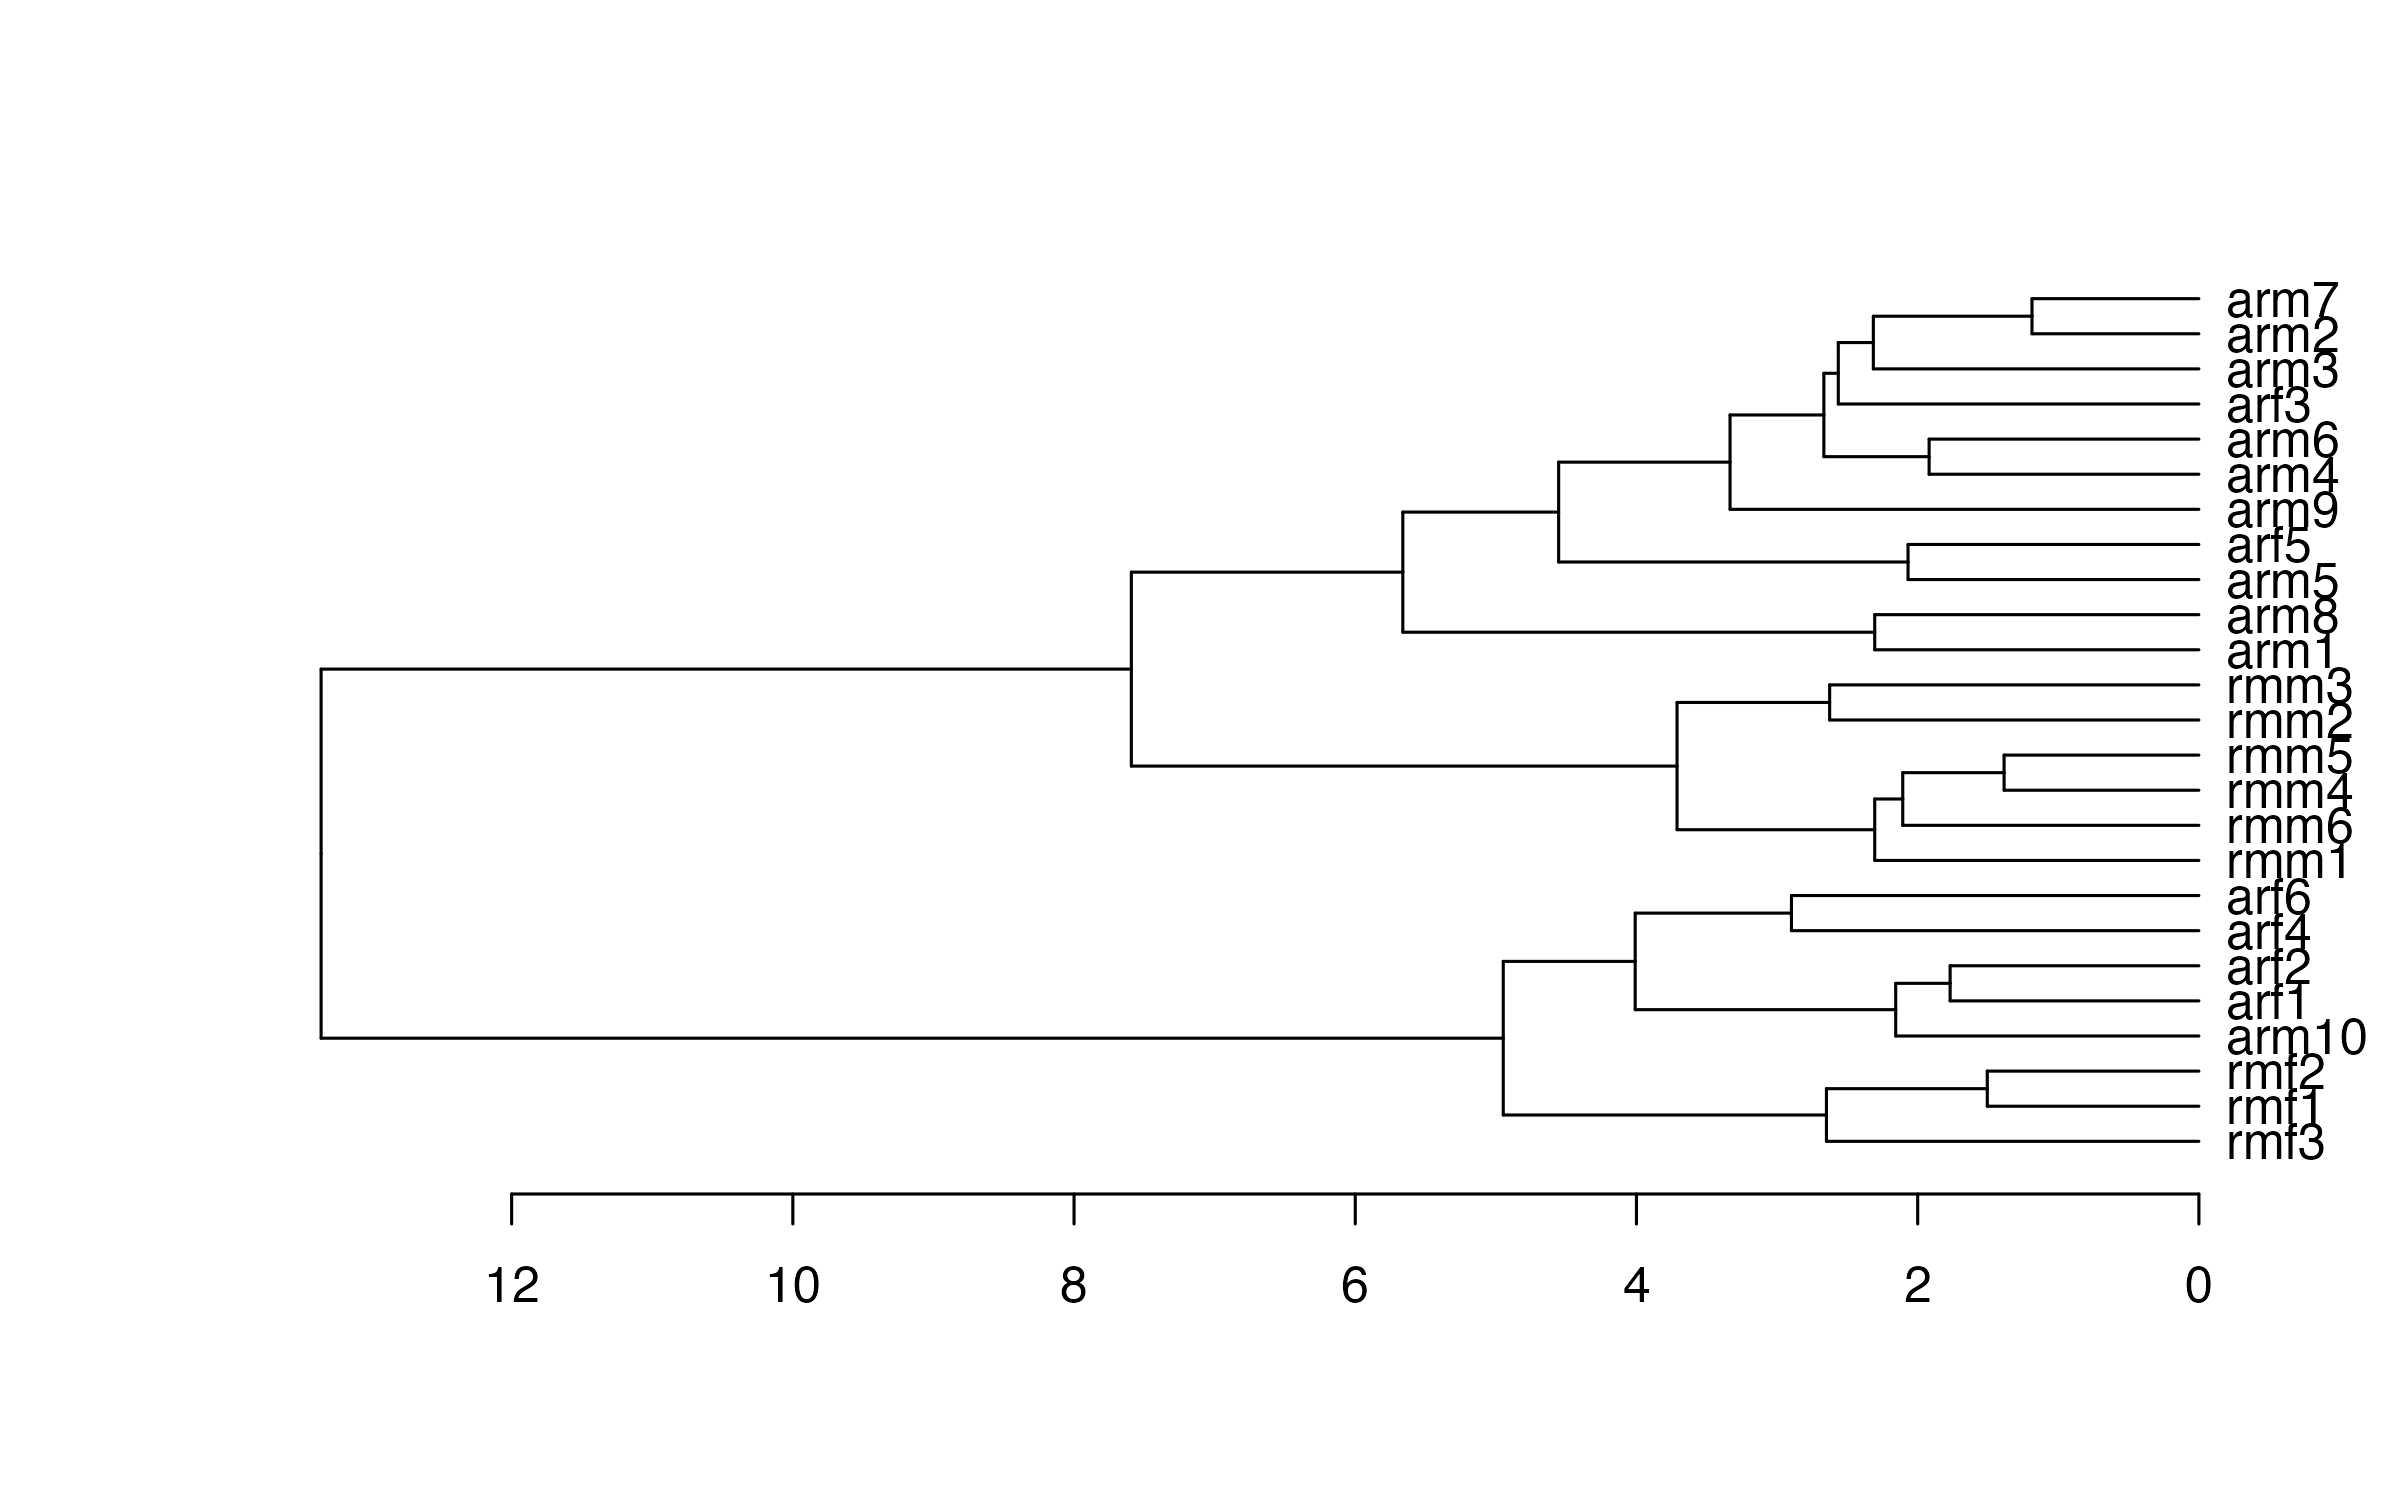
\includegraphics[keepaspectratio]{05_cluster_analysis_files/figure-beamer/fig-ward-dend-1.png}}

}

\caption{\label{fig-ward-dend}}

\end{figure}%
\end{frame}

\section{Качество
кластеризации}\label{ux43aux430ux447ux435ux441ux442ux432ux43e-ux43aux43bux430ux441ux442ux435ux440ux438ux437ux430ux446ux438ux438}

\begin{frame}{Кофенетическая корреляция: расчёт}
\protect\phantomsection\label{ux43aux43eux444ux435ux43dux435ux442ux438ux447ux435ux441ux43aux430ux44f-ux43aux43eux440ux440ux435ux43bux44fux446ux438ux44f-ux440ux430ux441ux447ux451ux442}
\textbf{Кофенетическое расстояние} ----- расстояние между объектами на
дендрограмме, т.е. то расстояние, на котором объекты становятся частью
одной группы в ходе процесса кластеризации.

\begin{block}{}
\textbf{Кофенетическая корреляция}  —-- мера качества отображения многомерных данных на дендрограмме. Кофенетическую корреляцию можно рассчитать как Пирсоновскую корреляцию (обычную) между матрицами исходных и кофенетических расстояний между всеми парами объектов. В идеальном случае равна 1. 
\end{block}

\[r = \frac{\sum_{i<j}(d_{ij} - \bar{d})(c_{ij} - \bar{c})}
{\sqrt{\sum_{i<j}(d_{ij}-\bar{d})^2 \cdot \sum_{i<j}(c_{ij}-\bar{c})^2}}\]

где:

\begin{itemize}
\tightlist
\item
  \(d_{ij}\) --- исходное расстояние между объектами \(i\) и \(j\),
\item
  \(c_{ij}\) --- кофенетическое расстояние между объектами \(i\) и
  \(j\),
\item
  \(\bar{d}\) --- среднее исходных расстояний,
\item
  \(\bar{c}\) --- среднее кофенетических расстояний.
\end{itemize}
\end{frame}

\begin{frame}[fragile]{Кофенетическая корреляция: смысл}
\protect\phantomsection\label{ux43aux43eux444ux435ux43dux435ux442ux438ux447ux435ux441ux43aux430ux44f-ux43aux43eux440ux440ux435ux43bux44fux446ux438ux44f-ux441ux43cux44bux441ux43b}
Метод агрегации, который дает наибольшую кофенетическую корреляцию, дает
кластеры, лучше всего отражающие исходные данные.

Матрицу кофенетических расстояний и кофенетическую корреляцию можно
рассчитать при помощи функций из пакета \texttt{stats}
(\texttt{dendextend}) и \texttt{ape}, соответственно.
\end{frame}

\begin{frame}[fragile]{Кофенетическая корреляция в R}
\protect\phantomsection\label{ux43aux43eux444ux435ux43dux435ux442ux438ux447ux435ux441ux43aux430ux44f-ux43aux43eux440ux440ux435ux43bux44fux446ux438ux44f-ux432-r}
\scriptsize

\begin{Shaded}
\begin{Highlighting}[]
\CommentTok{\# Матрица кофенетических расстояний }
\NormalTok{c\_single }\OtherTok{\textless{}{-}} \FunctionTok{cophenetic}\NormalTok{(ph\_single)}

\CommentTok{\# Кофенетическая корреляция = }
\CommentTok{\# = корреляция матриц кофенетич. и реальн. расстояний}
\FunctionTok{cor}\NormalTok{(d, }\FunctionTok{as.dist}\NormalTok{(c\_single))}
\end{Highlighting}
\end{Shaded}

\begin{verbatim}
[1] 0.5654072
\end{verbatim}
\end{frame}

\begin{frame}{Задание:}
\protect\phantomsection\label{ux437ux430ux434ux430ux43dux438ux435-1}
Оцените при помощи кофенетической корреляции качество кластеризаций,
полученных разными методами.

Какой метод дает лучший результат?
\end{frame}

\begin{frame}[fragile]{Решение}
\protect\phantomsection\label{ux440ux435ux448ux435ux43dux438ux435-2}
\scriptsize

\begin{Shaded}
\begin{Highlighting}[]
\NormalTok{c\_single }\OtherTok{\textless{}{-}} \FunctionTok{cophenetic}\NormalTok{(ph\_single)}
\FunctionTok{cor}\NormalTok{(d, }\FunctionTok{as.dist}\NormalTok{(c\_single))}
\end{Highlighting}
\end{Shaded}

\begin{verbatim}
[1] 0.5654072
\end{verbatim}

\begin{Shaded}
\begin{Highlighting}[]
\NormalTok{c\_compl }\OtherTok{\textless{}{-}} \FunctionTok{cophenetic}\NormalTok{(ph\_compl)}
\FunctionTok{cor}\NormalTok{(d, }\FunctionTok{as.dist}\NormalTok{(c\_compl))}
\end{Highlighting}
\end{Shaded}

\begin{verbatim}
[1] 0.705757
\end{verbatim}

\begin{Shaded}
\begin{Highlighting}[]
\NormalTok{c\_avg }\OtherTok{\textless{}{-}} \FunctionTok{cophenetic}\NormalTok{(ph\_avg)}
\FunctionTok{cor}\NormalTok{(d, }\FunctionTok{as.dist}\NormalTok{(c\_avg))}
\end{Highlighting}
\end{Shaded}

\begin{verbatim}
[1] 0.7446591
\end{verbatim}

\begin{Shaded}
\begin{Highlighting}[]
\NormalTok{c\_w2 }\OtherTok{\textless{}{-}} \FunctionTok{cophenetic}\NormalTok{(ph\_w2)}
\FunctionTok{cor}\NormalTok{(d, }\FunctionTok{as.dist}\NormalTok{(c\_w2))}
\end{Highlighting}
\end{Shaded}

\begin{verbatim}
[1] 0.7259618
\end{verbatim}
\end{frame}

\begin{frame}{Что можно делать дальше с дендрограммой}
\protect\phantomsection\label{ux447ux442ux43e-ux43cux43eux436ux43dux43e-ux434ux435ux43bux430ux442ux44c-ux434ux430ux43bux44cux448ux435-ux441-ux434ux435ux43dux434ux440ux43eux433ux440ux430ux43cux43cux43eux439}
\begin{itemize}
\tightlist
\item
  Можно выбрать число кластеров:

  \begin{itemize}
  \tightlist
  \item
    либо субъективно, на любом выбранном уровне (главное, чтобы кластеры
    были осмысленными и интерпретируемыми);
  \item
    либо исходя из распределения расстояний ветвления.
  \end{itemize}
\item
  Можно оценить стабильность кластеризации при помощи бутстрепа.
\end{itemize}
\end{frame}

\begin{frame}{Ширина силуэта}
\protect\phantomsection\label{ux448ux438ux440ux438ux43dux430-ux441ux438ux43bux443ux44dux442ux430}
\begin{block}{}
Ширина силуэта $s_i$ --- мера степени принадлежности объекта $i$ к кластеру 
\end{block}

\[s_i = \frac {\color{purple}{\bar{d}_{i~to~nearest~cluster}} - \color{green}{\bar{d}_{i~within}}} {max\{\color{purple}{\bar{d}_{i~to~nearest~cluster}}, \color{green}{\bar{d}_{i~within}}\}}\]

\(s_i\) --- сравнивает между собой средние расстояния от данного
объекта:

\begin{itemize}
\tightlist
\item
  \(\color{green} {\bar{d}_{i~within}}\) --- до других объектов из того
  же кластера
\item
  \(\color{purple} {\bar{d}_{i~to~nearest~cluster}}\) --- до ближайшего
  кластера
\end{itemize}

\(-1 \le s_i \le 1\) --- чем больше \(s_i\), тем ``лучше'' объект
принадлежит кластеру.

\begin{itemize}
\tightlist
\item
  Средняя ширина силуэта для всех объектов из кластера --- оценивает,
  насколько ``тесно'' сгруппированы объекты.
\item
  Средняя ширина силуэта по всем данным --- оценивает общее качество
  классификации.
\item
  Чем больше к 1, тем лучше. Если меньше 0.25, то можно сказать, что нет
  структуры.
\end{itemize}
\end{frame}

\begin{frame}[fragile]{Как рассчитывается ширина силуэта}
\protect\phantomsection\label{ux43aux430ux43a-ux440ux430ux441ux441ux447ux438ux442ux44bux432ux430ux435ux442ux441ux44f-ux448ux438ux440ux438ux43dux430-ux441ux438ux43bux443ux44dux442ux430}
Оценим ширину силуэта для 3 кластеров

\begin{Shaded}
\begin{Highlighting}[]
\FunctionTok{library}\NormalTok{(cluster)}
\NormalTok{avg3 }\OtherTok{\textless{}{-}} \FunctionTok{cutree}\NormalTok{(}\AttributeTok{tree =}\NormalTok{ hc\_avg, }\AttributeTok{k =} \DecValTok{3}\NormalTok{) }\CommentTok{\# делим дерево на нужное количество кластеров}
\FunctionTok{plot}\NormalTok{(}\FunctionTok{silhouette}\NormalTok{(}\AttributeTok{x =}\NormalTok{ avg3, }\AttributeTok{dist =}\NormalTok{ d), }\AttributeTok{cex.names =} \FloatTok{0.6}\NormalTok{)}
\end{Highlighting}
\end{Shaded}

\begin{figure}[H]

\centering{

\pandocbounded{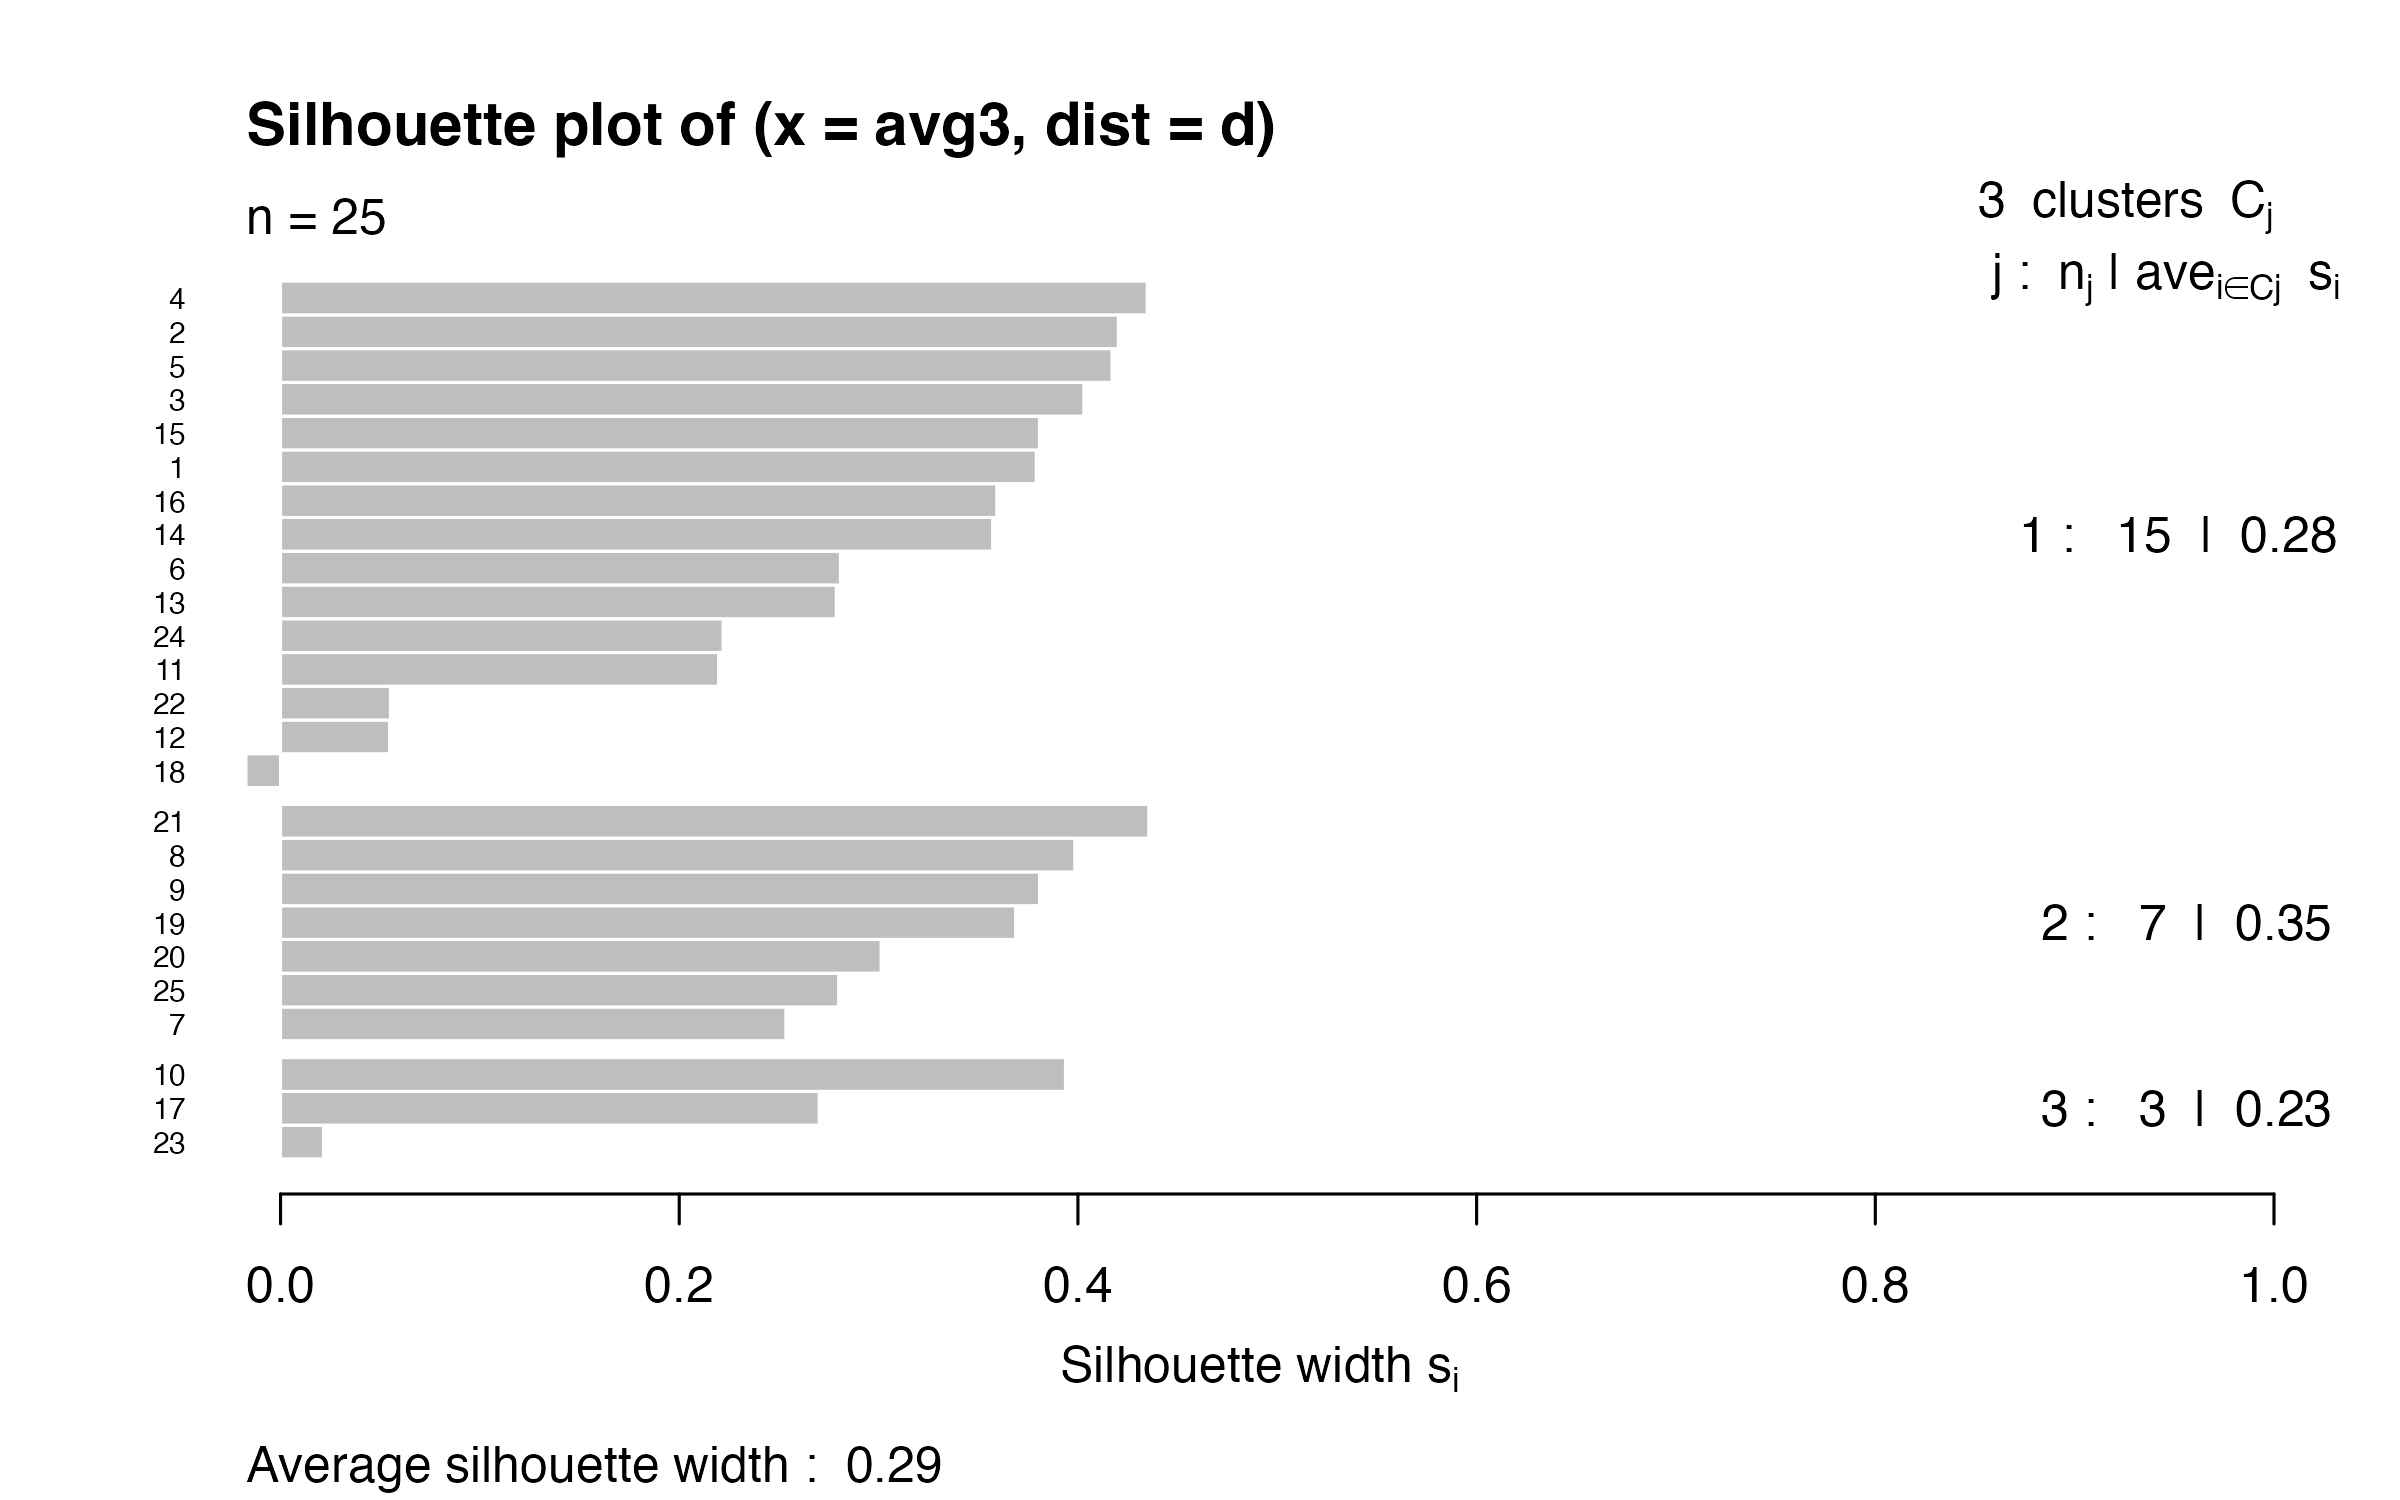
\includegraphics[keepaspectratio]{05_cluster_analysis_files/figure-beamer/fig-silhouette-1.png}}

}

\caption{\label{fig-silhouette}}

\end{figure}%
\end{frame}

\begin{frame}{Бутстреп}
\protect\phantomsection\label{ux431ux443ux442ux441ux442ux440ux435ux43f}
\begin{block}{}
\textbf{Бутстреп} --- один из методов оценки значимости полученных результатов; повторная выборка из имеющихся данных. В такой выборке элементы могут повторяться.
\end{block}

\textbf{Алгоритм}

\begin{itemize}
\tightlist
\item
  Имеющиеся данные делим на группы одинакового размера: какие-то
  элементы могут отсутствовать, а какие-то --- повторяться несколько
  раз.
\item
  На основе полученных данных строим дендрограмму.
\item
  Повторяем всё много раз.
\end{itemize}
\end{frame}

\begin{frame}[fragile]{Бутстреп поддержка ветвей}
\protect\phantomsection\label{ux431ux443ux442ux441ux442ux440ux435ux43f-ux43fux43eux434ux434ux435ux440ux436ux43aux430-ux432ux435ux442ux432ux435ux439}
\begin{quote}
``An approximately unbiased test of phylogenetic tree selection.''

--- Shimodaria, 2002
\end{quote}

Этот тест использует специальный вариант бутстрепа --- multiscale
bootstrap. Мы не просто многократно берем бутстреп-выборки и оцениваем
для них вероятность получения топологий (BP p-value), эти выборки еще и
будут с разным числом объектов. По изменению BP при разных объемах
выборки можно вычислить AU (approximately unbiased p-value). BP
недооценивает поддержку истинной топологии из-за дискретности повторных
выборок.

\scriptsize

\begin{Shaded}
\begin{Highlighting}[]
\FunctionTok{library}\NormalTok{(pvclust)}
\FunctionTok{set.seed}\NormalTok{(}\DecValTok{389}\NormalTok{)}
\CommentTok{\# итераций должно быть 1000 и больше, здесь мало для скорости}
\NormalTok{cl\_boot }\OtherTok{\textless{}{-}} \FunctionTok{pvclust}\NormalTok{(}\FunctionTok{t}\NormalTok{(st\_w), }\AttributeTok{method.hclust =} \StringTok{"average"}\NormalTok{, }\AttributeTok{nboot =} \DecValTok{100}\NormalTok{, }
                   \AttributeTok{method.dist =} \StringTok{"euclidean"}\NormalTok{, }\AttributeTok{parallel =} \ConstantTok{TRUE}\NormalTok{, }\AttributeTok{iseed =} \DecValTok{42}\NormalTok{)}
\end{Highlighting}
\end{Shaded}

\footnotesize

Обратите внимание на число итераций: \texttt{nboot\ =\ 100} --- это
очень мало. На самом деле нужно 10000 или больше.
\end{frame}

\begin{frame}[fragile]{Дерево с величинами поддержки}
\protect\phantomsection\label{ux434ux435ux440ux435ux432ux43e-ux441-ux432ux435ux43bux438ux447ux438ux43dux430ux43cux438-ux43fux43eux434ux434ux435ux440ux436ux43aux438}
AU --- approximately unbiased p-values (красный), BP --- bootstrap
p-values (зеленый).

\begin{Shaded}
\begin{Highlighting}[]
\FunctionTok{plot}\NormalTok{(cl\_boot)}
\FunctionTok{pvrect}\NormalTok{(cl\_boot) }\CommentTok{\# достоверные ветвления}
\end{Highlighting}
\end{Shaded}

\begin{figure}[H]

\centering{

\pandocbounded{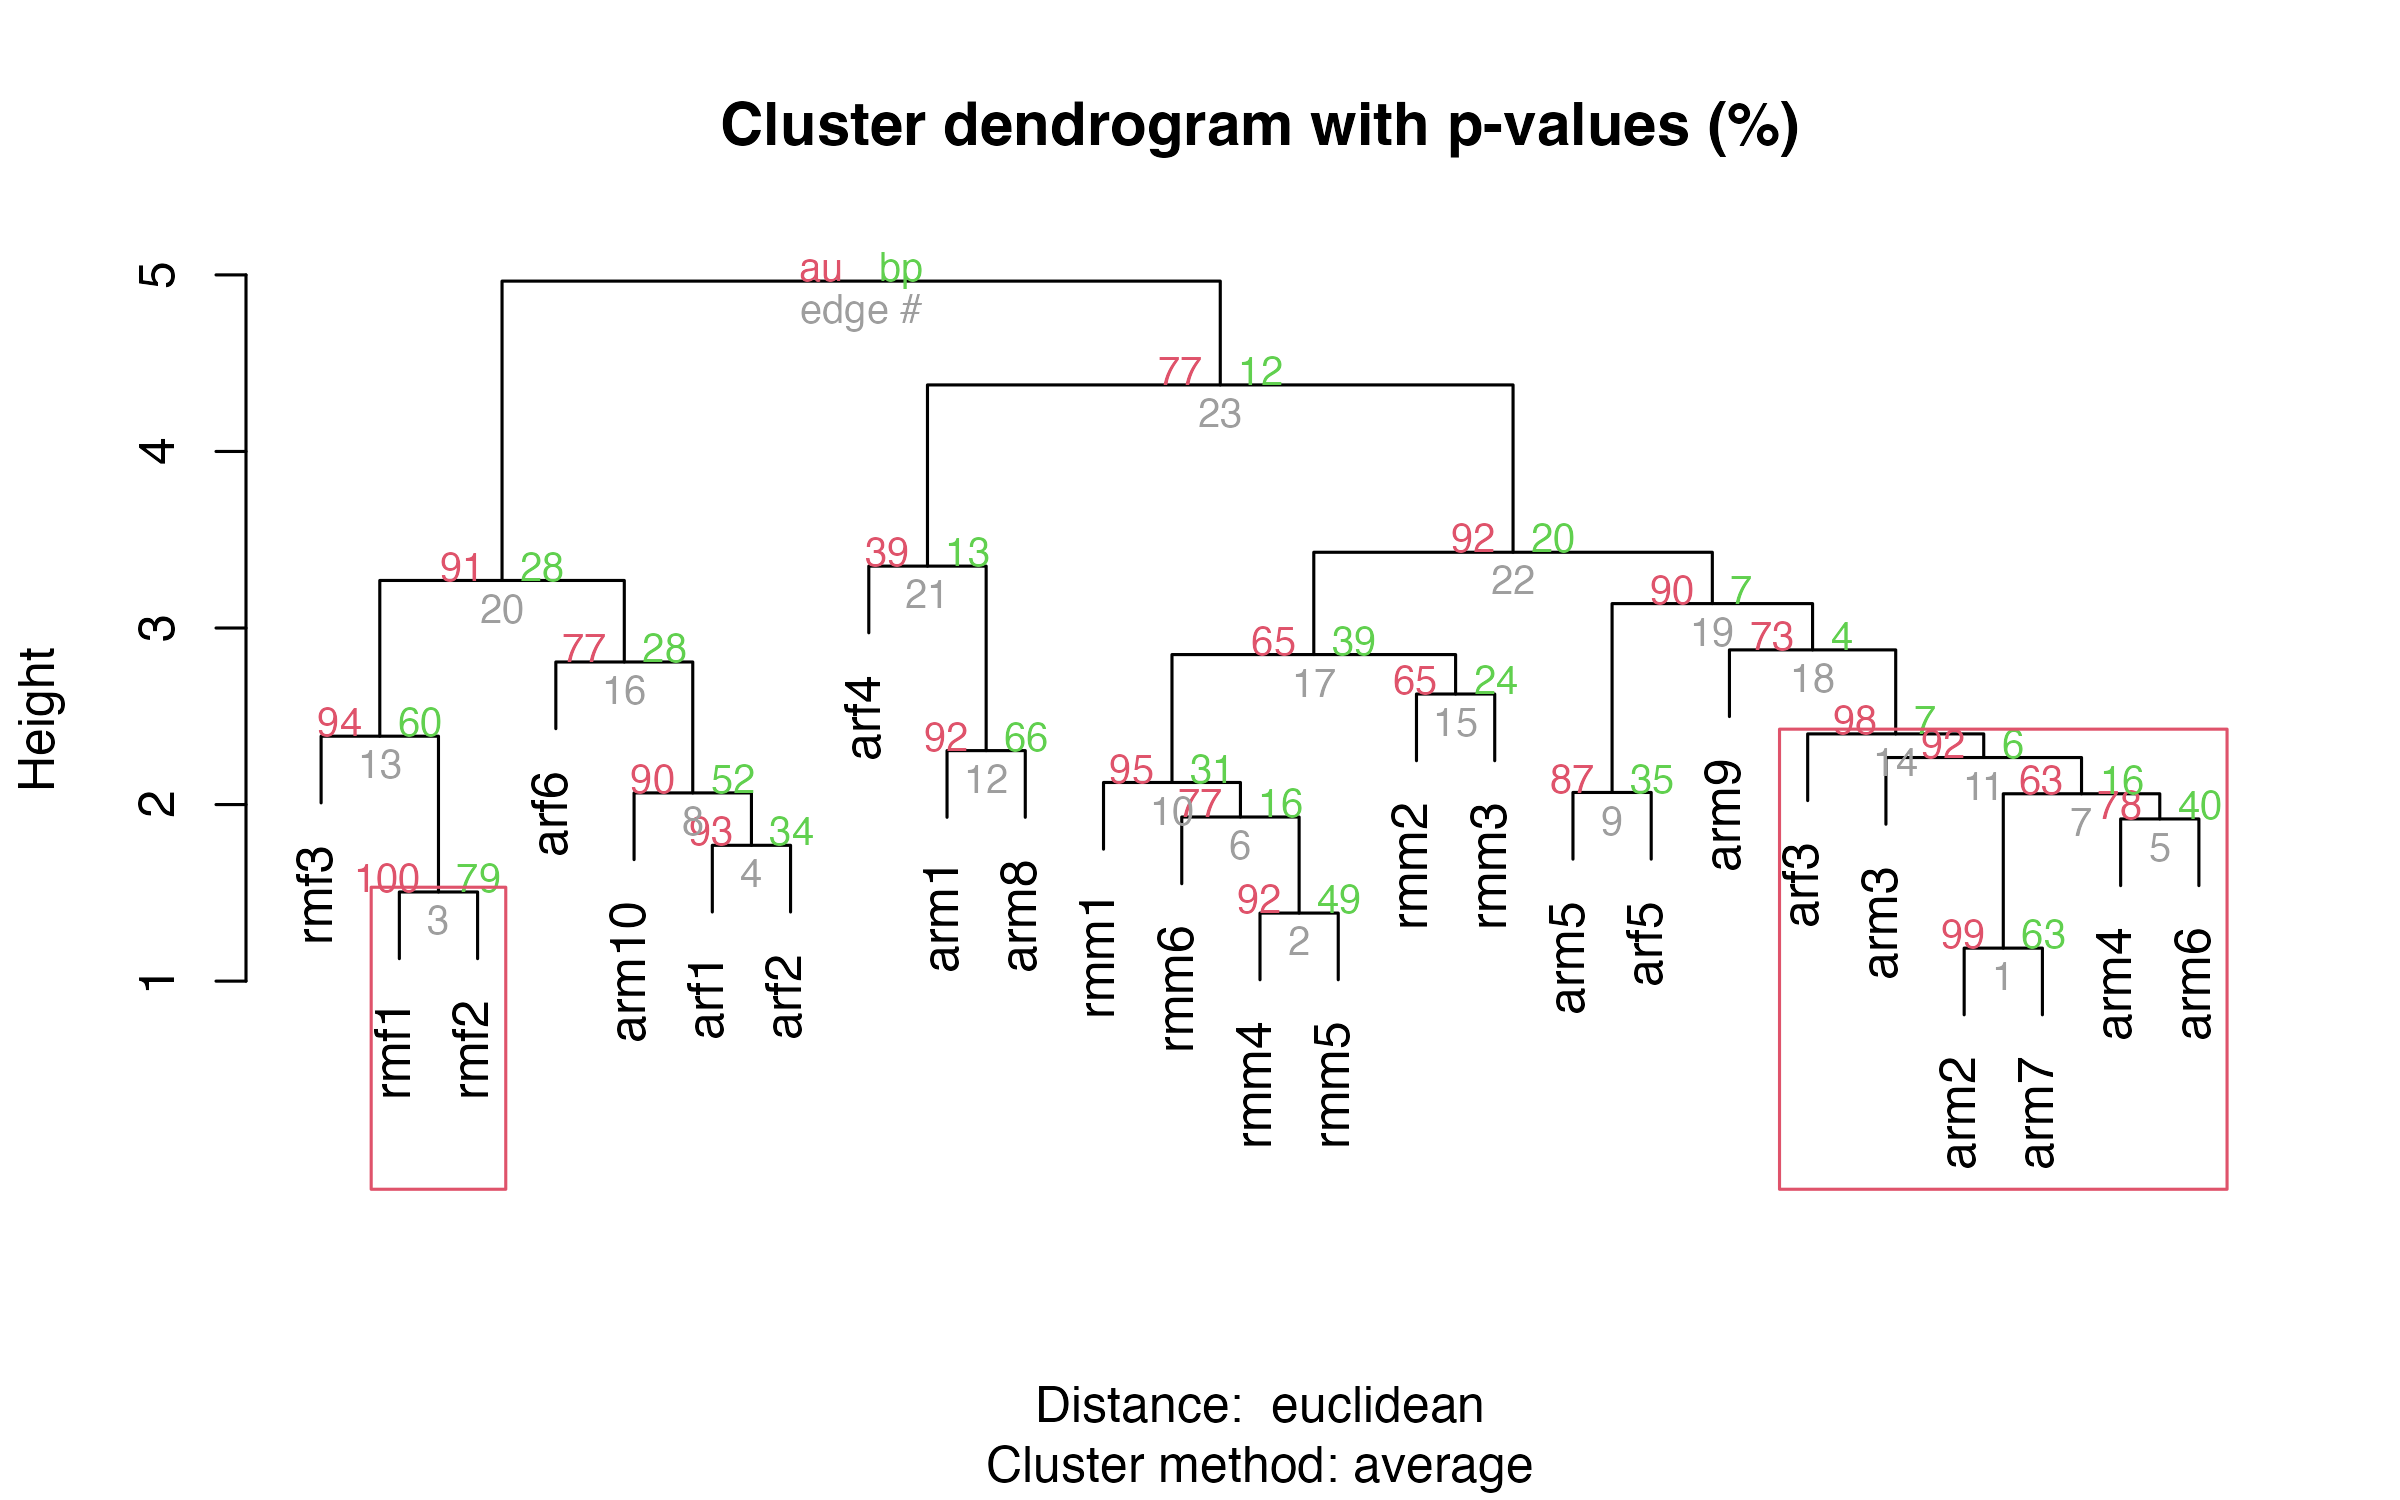
\includegraphics[keepaspectratio]{05_cluster_analysis_files/figure-beamer/fig-cl-boot-1.png}}

}

\caption{\label{fig-cl-boot}}

\end{figure}%
\end{frame}

\begin{frame}[fragile]{Для диагностики качества оценок AU}
\protect\phantomsection\label{ux434ux43bux44f-ux434ux438ux430ux433ux43dux43eux441ux442ux438ux43aux438-ux43aux430ux447ux435ux441ux442ux432ux430-ux43eux446ux435ux43dux43eux43a-au}
График стандартных ошибок для AU p-value нужен, чтобы оценить точность
оценки самих AU. Чем больше было бутстреп-итераций, тем точнее будет
оценка AU.

\begin{Shaded}
\begin{Highlighting}[]
\FunctionTok{seplot}\NormalTok{(cl\_boot)}
\CommentTok{\# print(cl\_boot) \# все значения}
\end{Highlighting}
\end{Shaded}

\begin{figure}[H]

\centering{

\pandocbounded{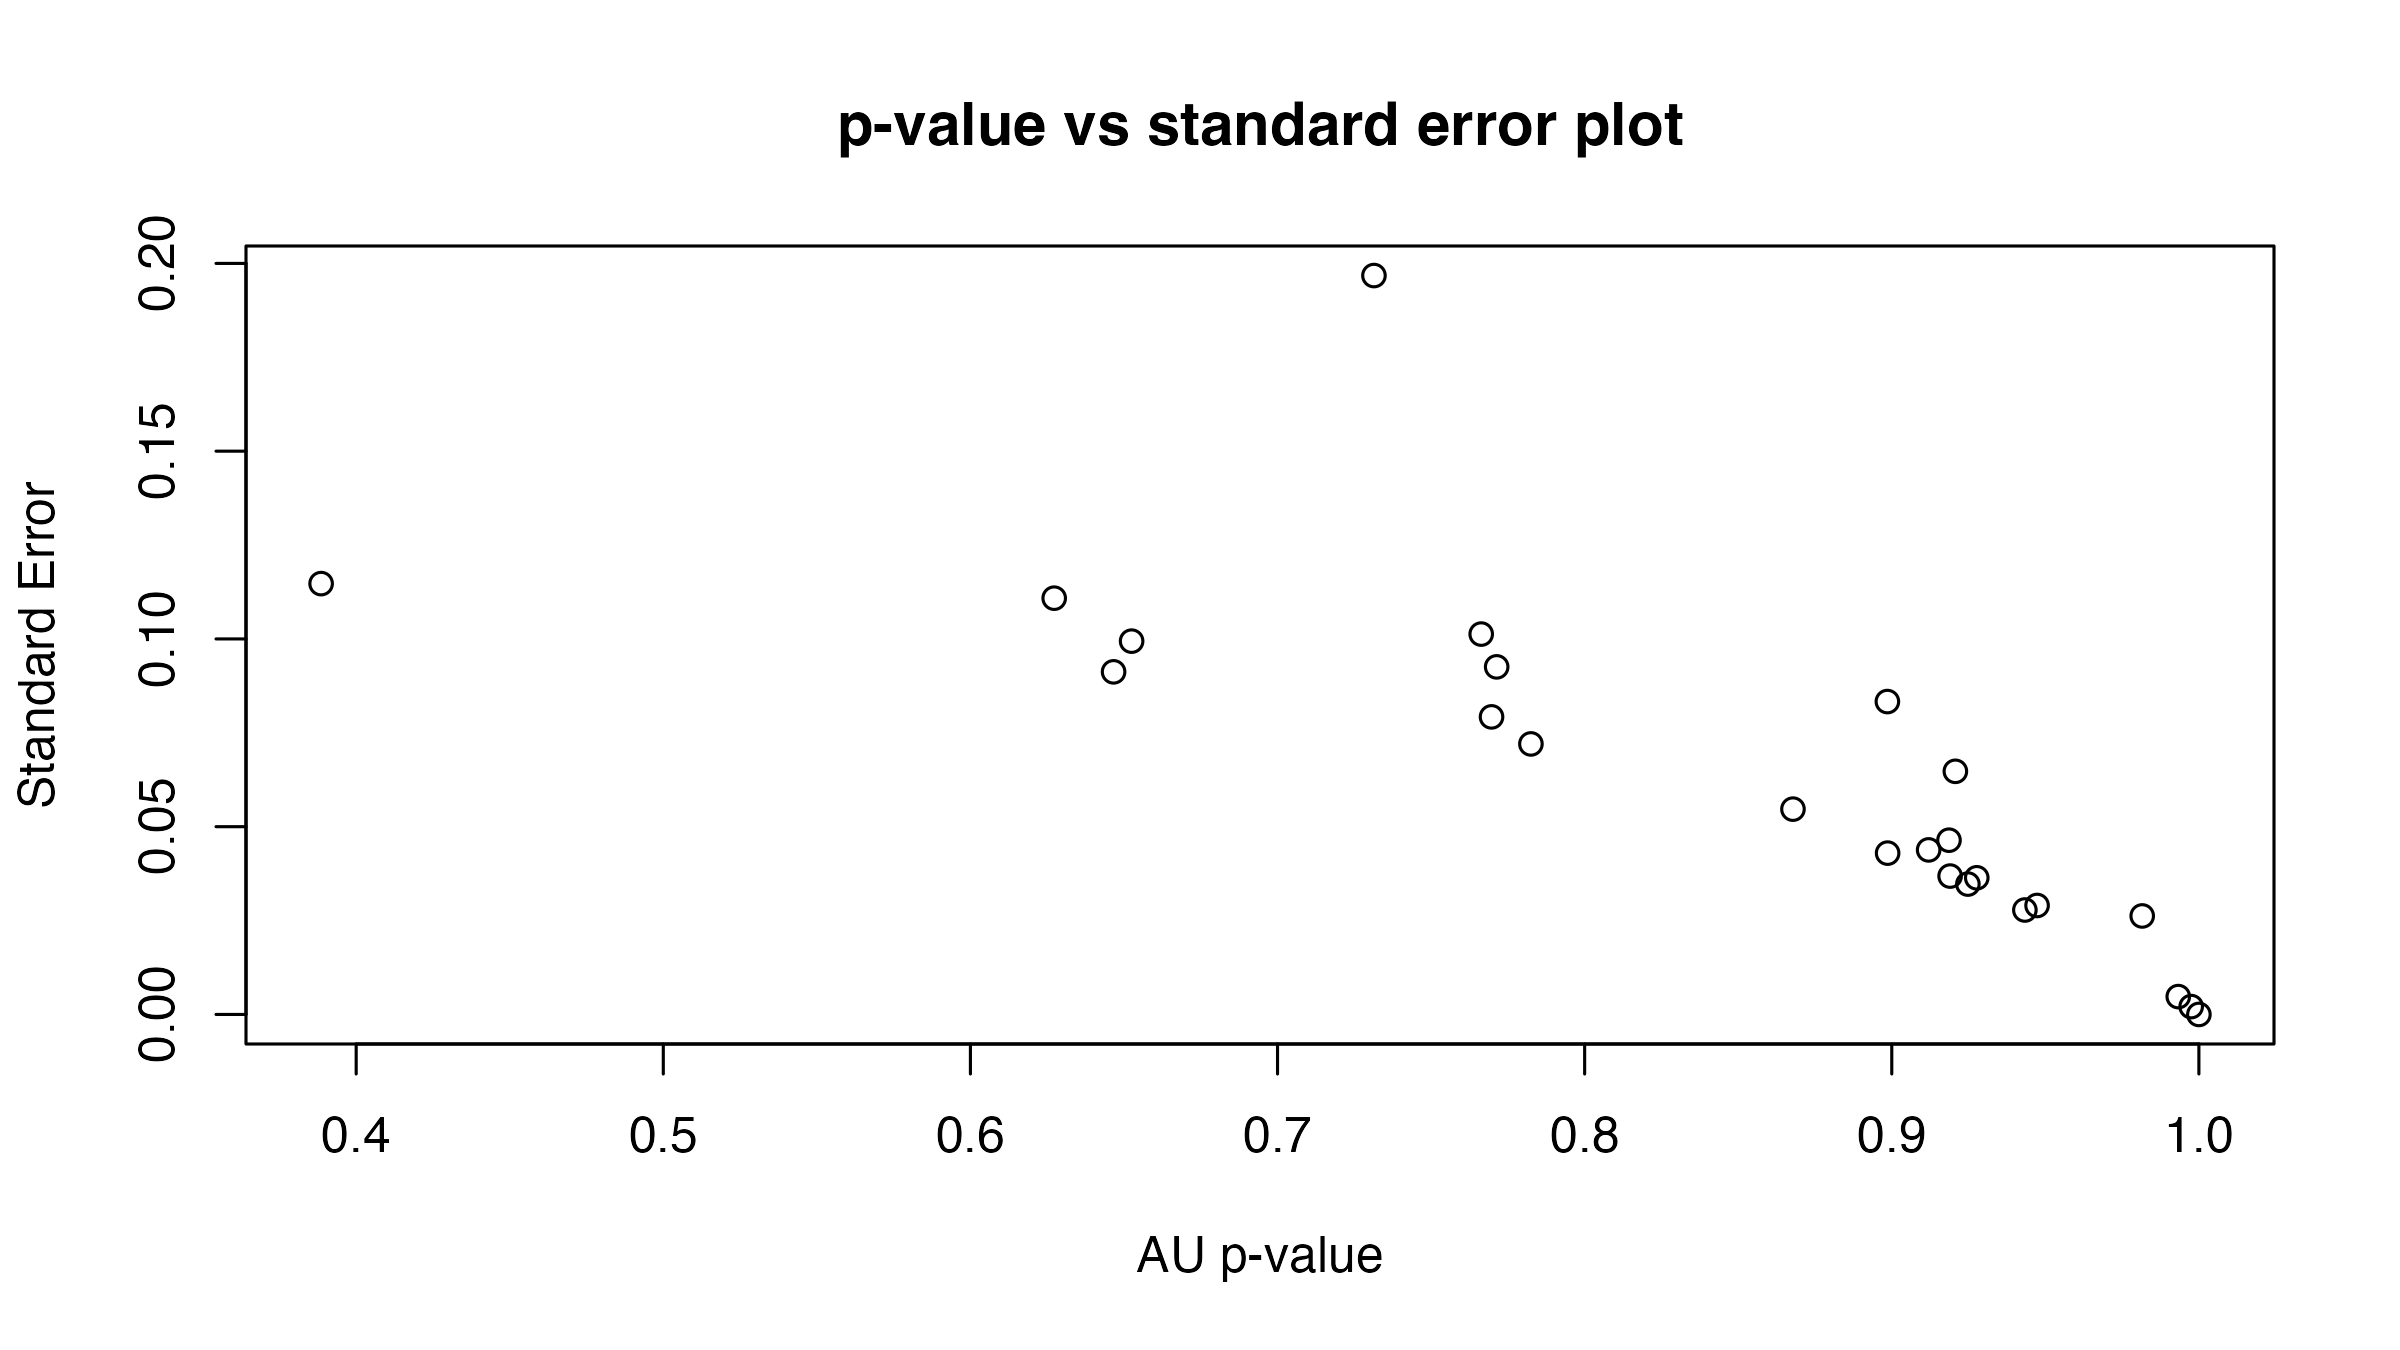
\includegraphics[keepaspectratio]{05_cluster_analysis_files/figure-beamer/fig-seplot-1.png}}

}

\caption{\label{fig-seplot}}

\end{figure}%
\end{frame}

\section{Сопоставление деревьев:
Танглграммы}\label{ux441ux43eux43fux43eux441ux442ux430ux432ux43bux435ux43dux438ux435-ux434ux435ux440ux435ux432ux44cux435ux432-ux442ux430ux43dux433ux43bux433ux440ux430ux43cux43cux44b}

\begin{frame}[fragile]{Танглграмма}
\protect\phantomsection\label{ux442ux430ux43dux433ux43bux433ux440ux430ux43cux43cux430}
Два дерева (с непохожим ветвлением) выравнивают, вращая случайным
образом ветви вокруг оснований. Итеративный алгоритм. Картина каждый раз
разная.

\begin{Shaded}
\begin{Highlighting}[]
\FunctionTok{set.seed}\NormalTok{(}\DecValTok{395}\NormalTok{)}
\NormalTok{untang\_w }\OtherTok{\textless{}{-}} \FunctionTok{untangle\_step\_rotate\_2side}\NormalTok{(den\_compl, den\_w2, }\AttributeTok{print\_times =}\NormalTok{ F)}

\CommentTok{\# танглграмма}
\FunctionTok{tanglegram}\NormalTok{(untang\_w[[}\DecValTok{1}\NormalTok{]], untang\_w[[}\DecValTok{2}\NormalTok{]],}
           \AttributeTok{highlight\_distinct\_edges =} \ConstantTok{FALSE}\NormalTok{,}
           \AttributeTok{common\_subtrees\_color\_lines =}\NormalTok{ F,}
           \AttributeTok{main =} \StringTok{"Tanglegram"}\NormalTok{,}
           \AttributeTok{main\_left =} \StringTok{"Left tree"}\NormalTok{,}
           \AttributeTok{main\_right =} \StringTok{"Right tree"}\NormalTok{,}
           \AttributeTok{columns\_width =} \FunctionTok{c}\NormalTok{(}\DecValTok{8}\NormalTok{, }\DecValTok{1}\NormalTok{, }\DecValTok{8}\NormalTok{),}
           \AttributeTok{margin\_top =} \FloatTok{3.2}\NormalTok{, }\AttributeTok{margin\_bottom =} \FloatTok{2.5}\NormalTok{,}
           \AttributeTok{margin\_inner =} \DecValTok{4}\NormalTok{, }\AttributeTok{margin\_outer =} \FloatTok{0.5}\NormalTok{,}
           \AttributeTok{lwd =} \FloatTok{1.2}\NormalTok{, }\AttributeTok{edge.lwd =} \FloatTok{1.2}\NormalTok{, }
           \AttributeTok{lab.cex =} \FloatTok{1.5}\NormalTok{, }\AttributeTok{cex\_main =} \DecValTok{2}\NormalTok{)}
\end{Highlighting}
\end{Shaded}
\end{frame}

\begin{frame}{Танглграмма}
\protect\phantomsection\label{ux442ux430ux43dux433ux43bux433ux440ux430ux43cux43cux430-1}
\begin{figure}

\centering{

\pandocbounded{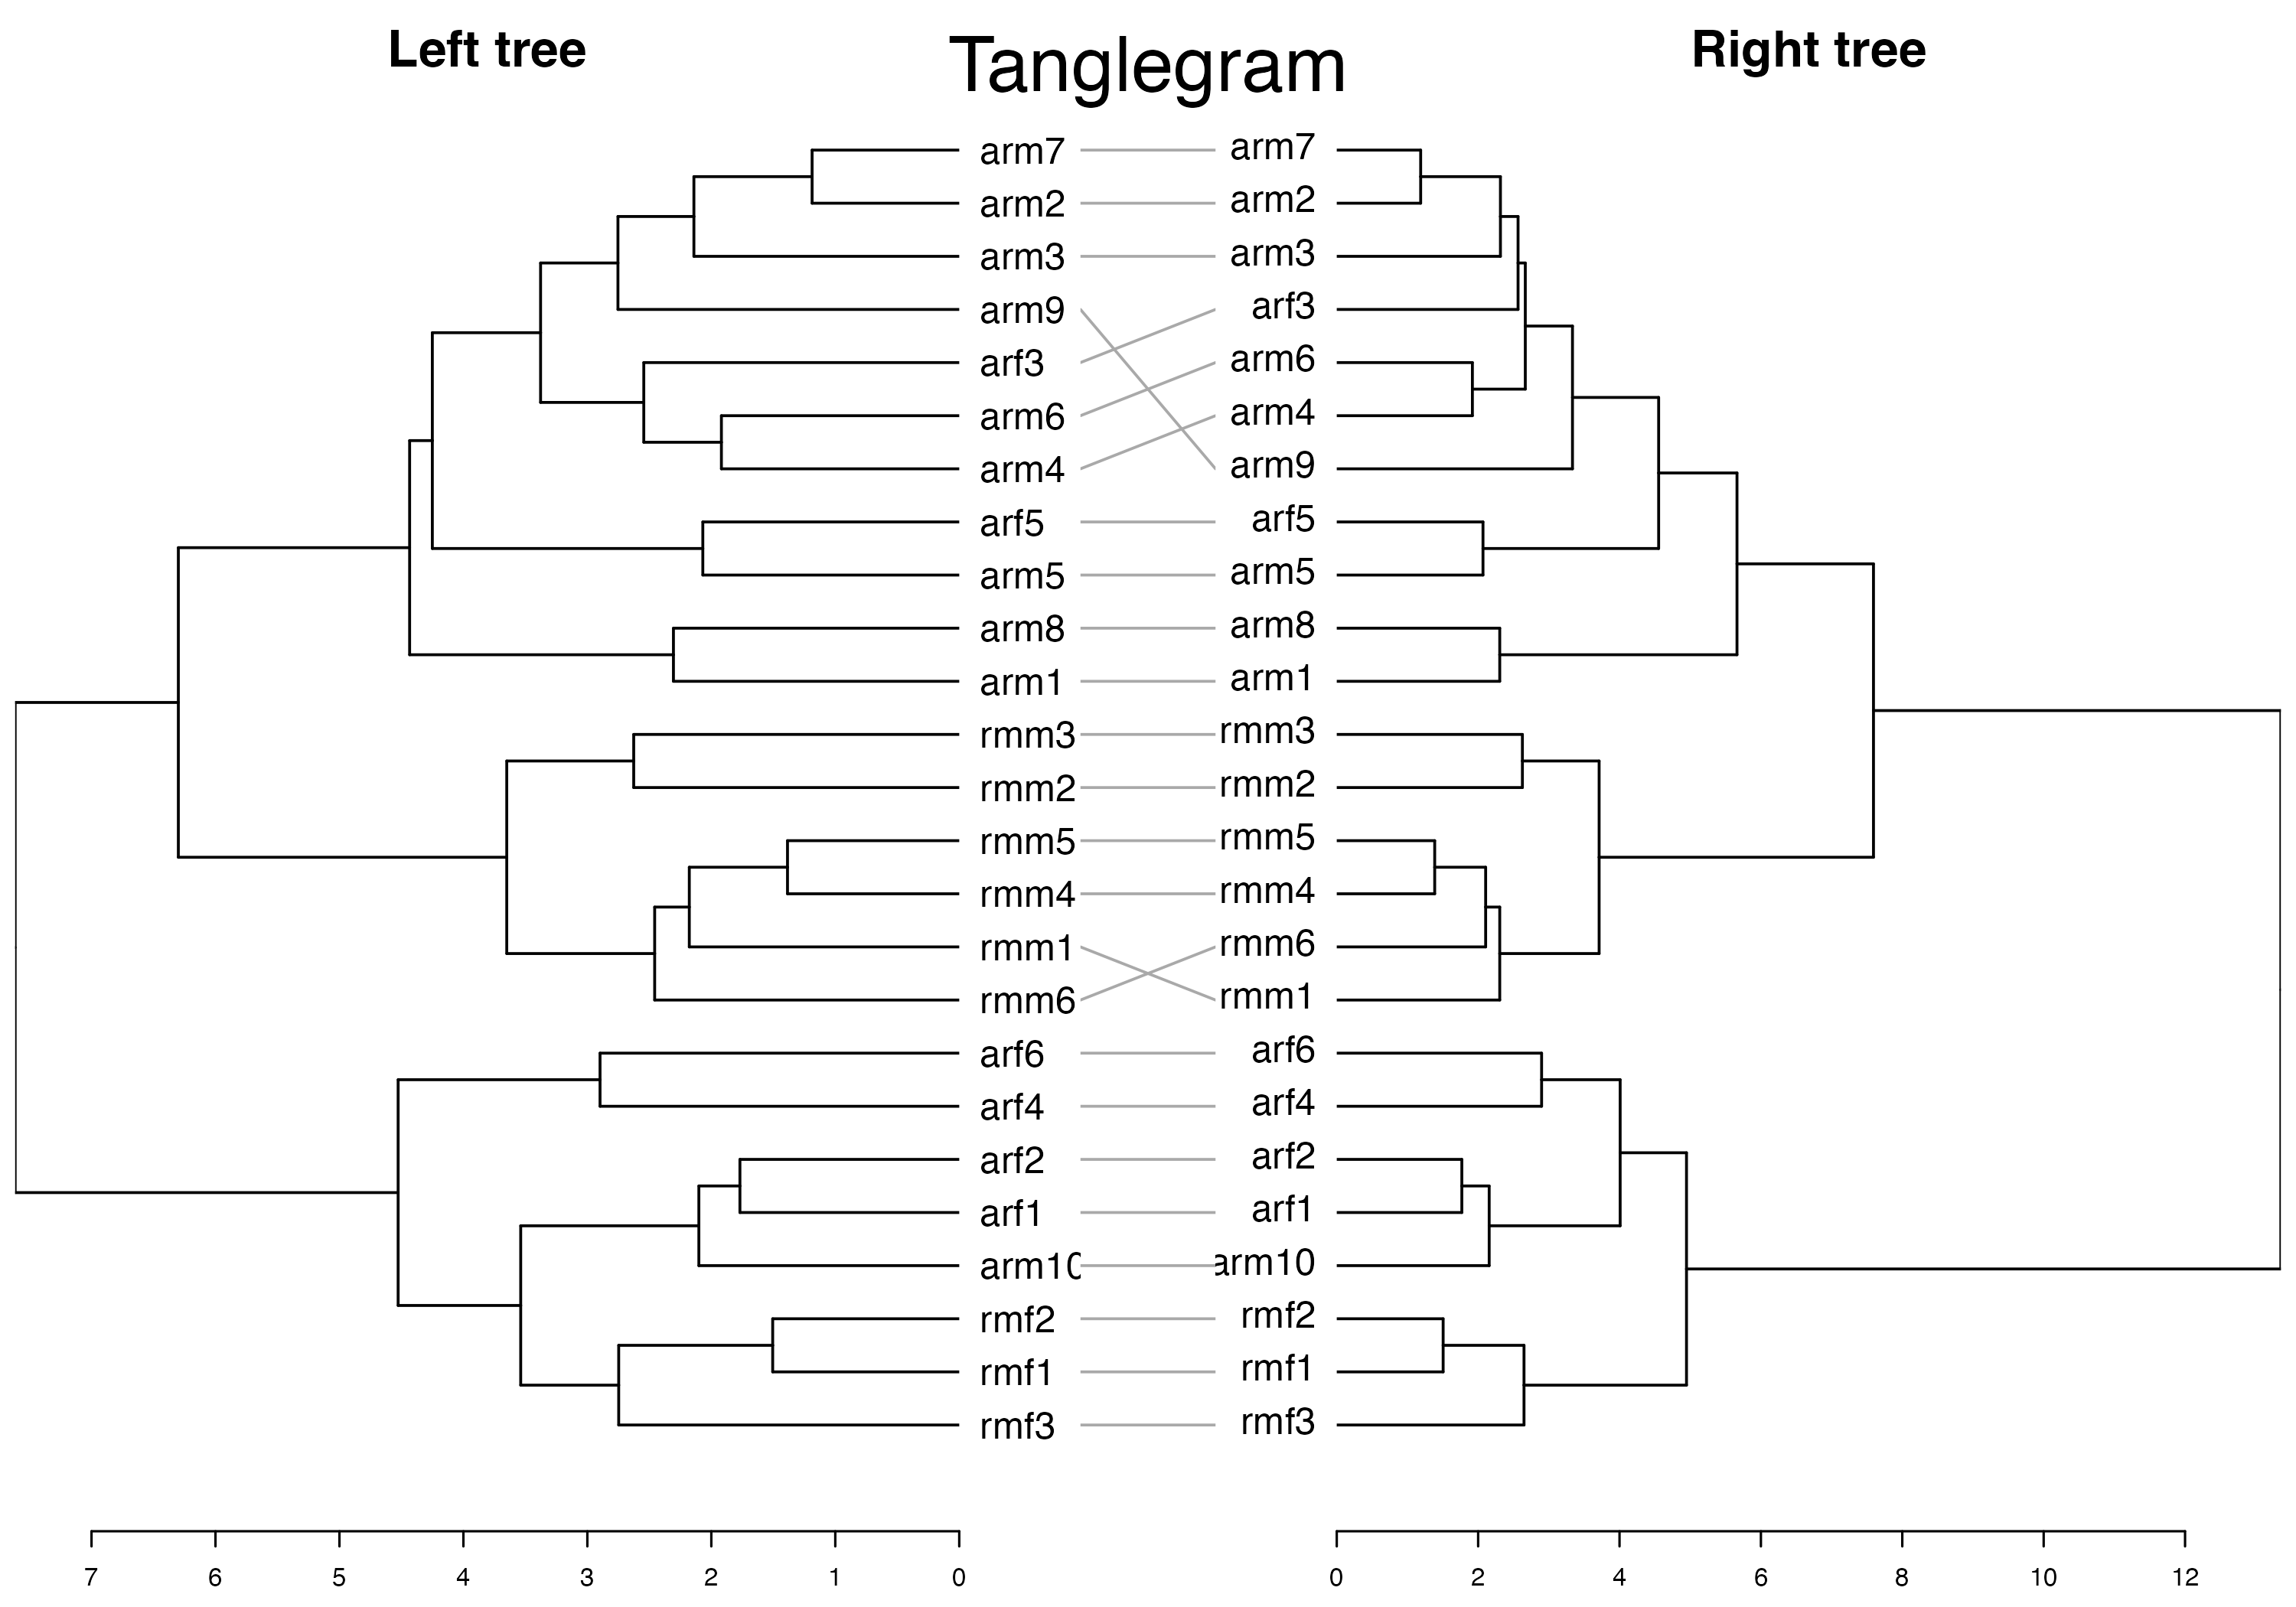
\includegraphics[keepaspectratio]{05_cluster_analysis_files/figure-beamer/fig-tang-1.png}}

}

\caption{\label{fig-tang}}

\end{figure}%
\end{frame}

\begin{frame}{Задание}
\protect\phantomsection\label{ux437ux430ux434ux430ux43dux438ux435-2}
Постройте танглграмму из дендрограмм, полученных методом ближайшего
соседа и методом Варда.
\end{frame}

\begin{frame}[fragile]{Раскраска дендрограмм}
\protect\phantomsection\label{ux440ux430ux441ux43aux440ux430ux441ux43aux430-ux434ux435ux43dux434ux440ux43eux433ux440ux430ux43cux43c}
\textbf{Вручную}

\begin{Shaded}
\begin{Highlighting}[]
\CommentTok{\# Произвольные цвета радуги}
\NormalTok{cols }\OtherTok{\textless{}{-}} \FunctionTok{rainbow}\NormalTok{(}\DecValTok{30}\NormalTok{) }
\NormalTok{den\_avg\_manual }\OtherTok{\textless{}{-}} \FunctionTok{color\_labels}\NormalTok{(}\AttributeTok{dend =}\NormalTok{ den\_avg, }\AttributeTok{col =}\NormalTok{ cols)}
\FunctionTok{plot}\NormalTok{(den\_avg\_manual, }\AttributeTok{horiz =} \ConstantTok{TRUE}\NormalTok{)}
\end{Highlighting}
\end{Shaded}

\pandocbounded{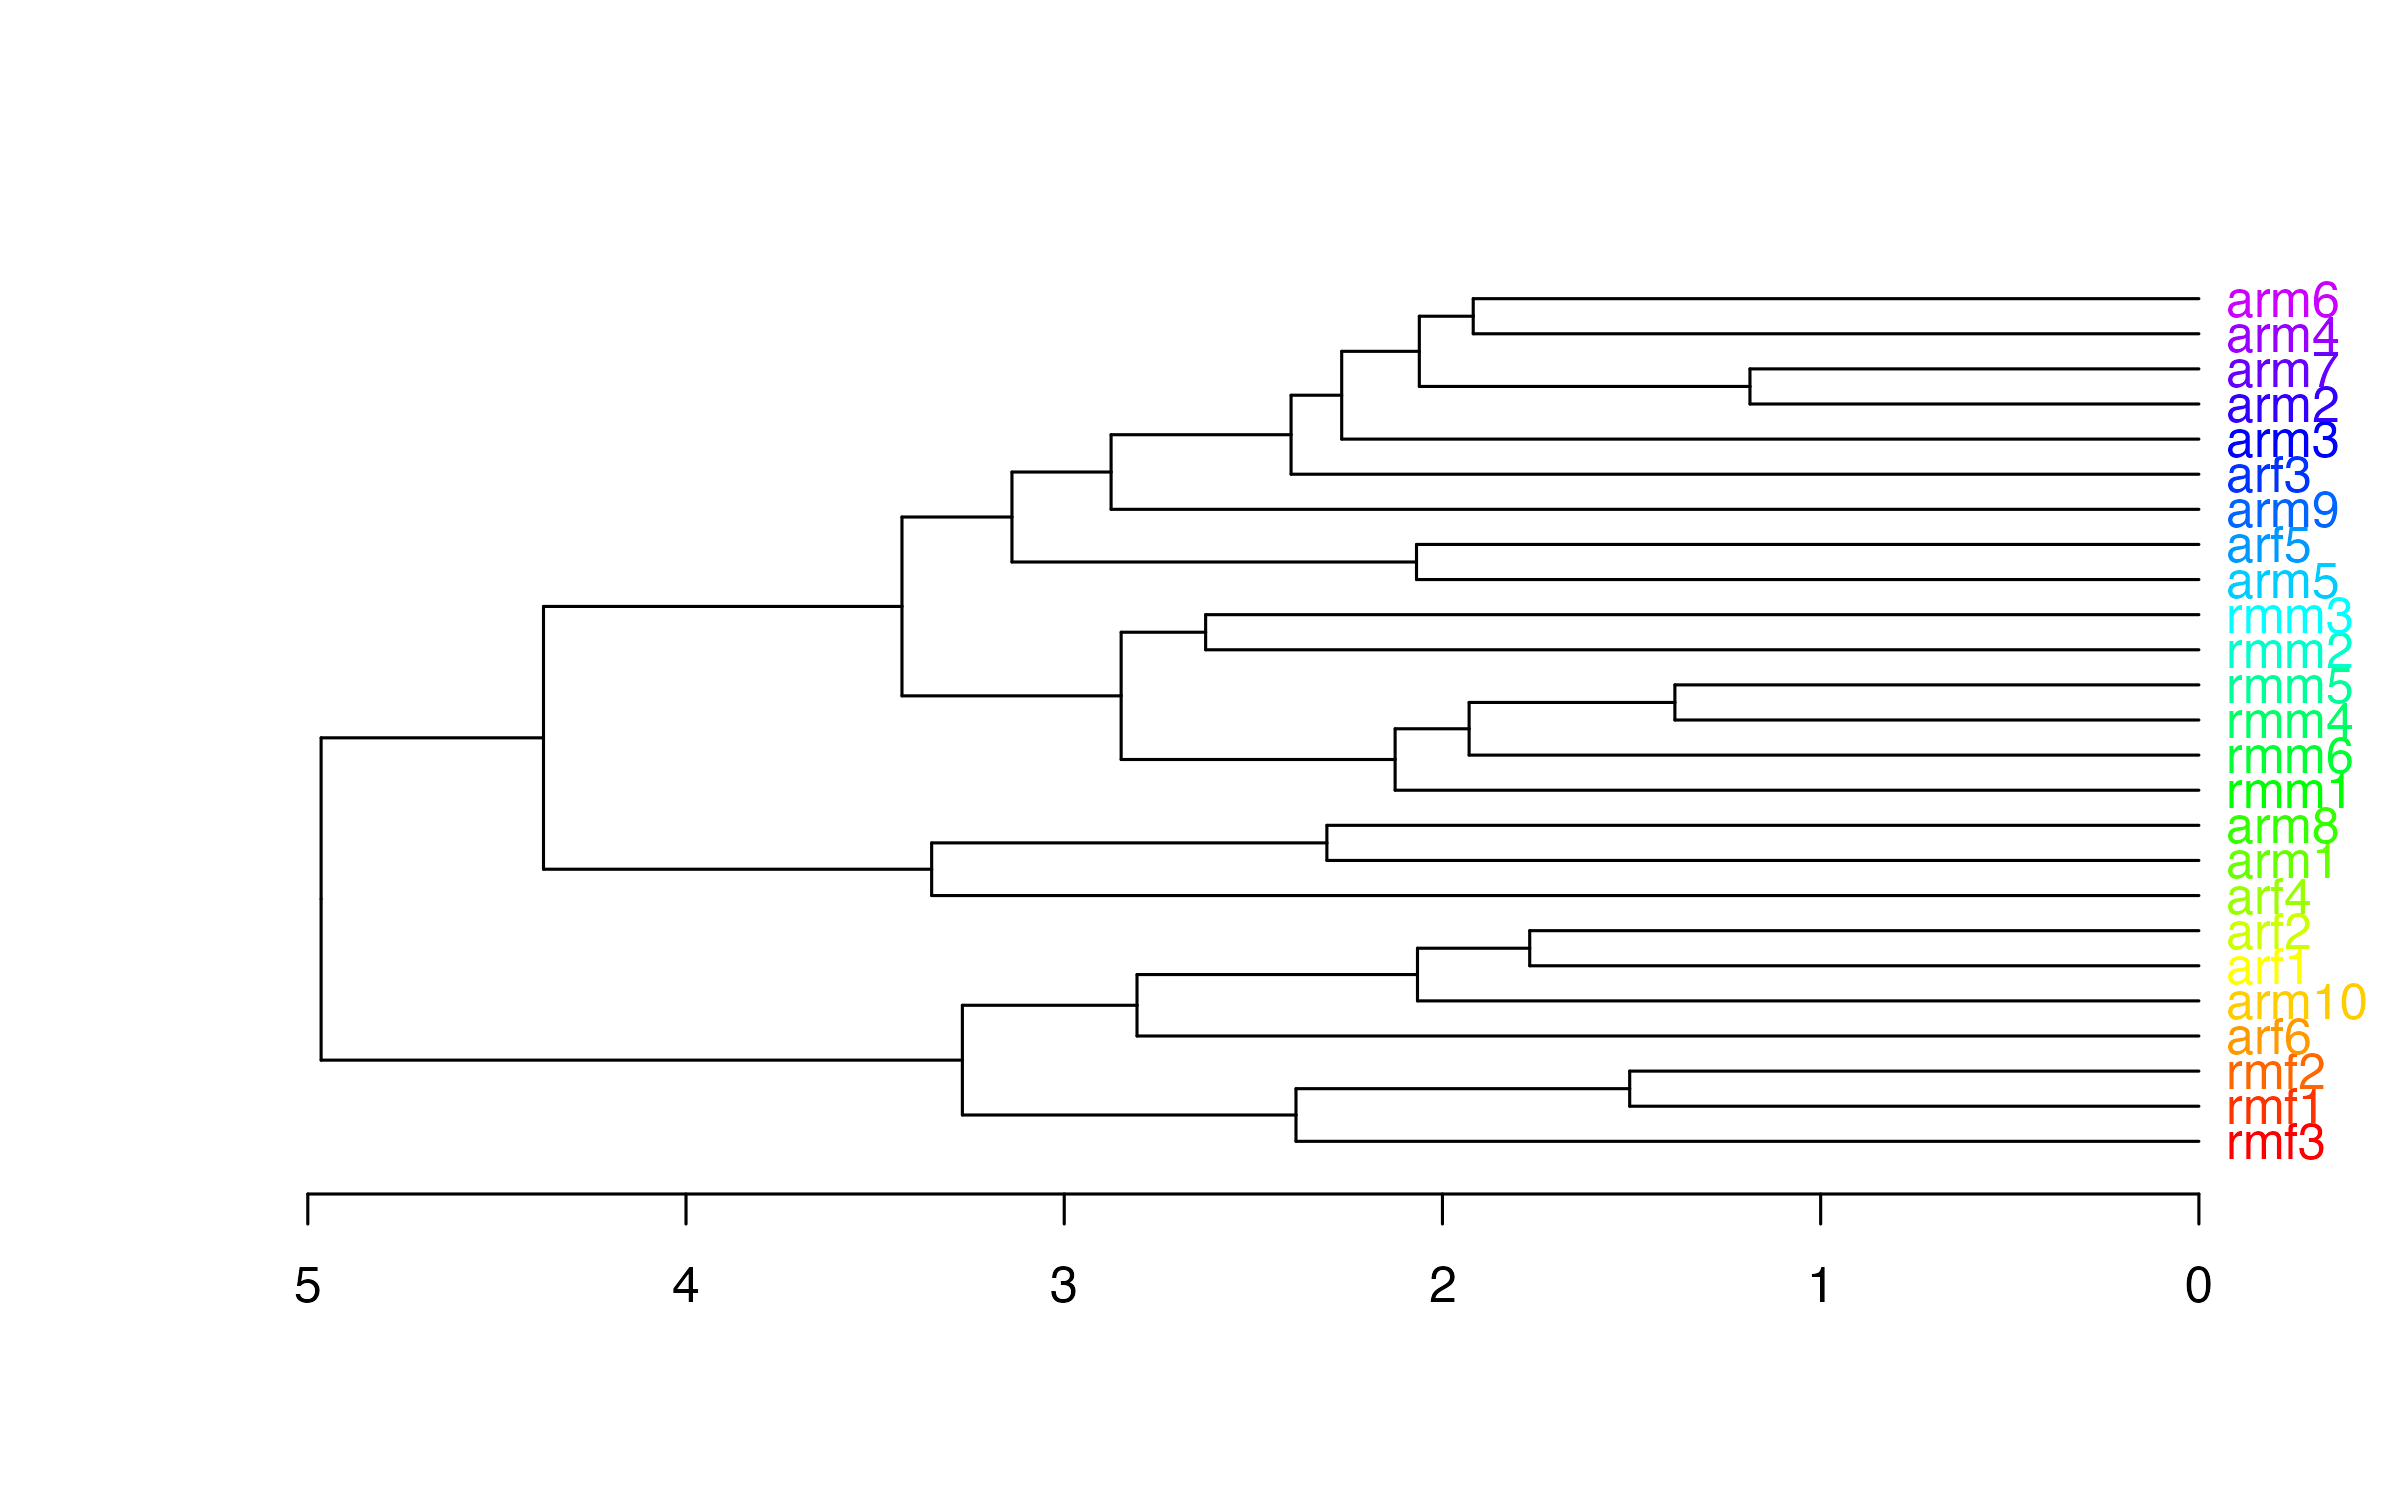
\includegraphics[keepaspectratio]{05_cluster_analysis_files/figure-beamer/unnamed-chunk-10-1.png}}
\end{frame}

\begin{frame}[fragile]{Раскраска дендрограмм}
\protect\phantomsection\label{ux440ux430ux441ux43aux440ux430ux441ux43aux430-ux434ux435ux43dux434ux440ux43eux433ux440ux430ux43cux43c-1}
\textbf{С помощью функции}

\begin{columns}[T]
\begin{column}{0.5\linewidth}
\begin{Shaded}
\begin{Highlighting}[]
\CommentTok{\# Функция для превращения лейблов в цвета}
\CommentTok{\# (группы определяются по \textasciigrave{}n\_chars\textasciigrave{} первых букв в лейбле)}
\NormalTok{get\_colours }\OtherTok{\textless{}{-}} \ControlFlowTok{function}\NormalTok{(dend, n\_chars, }\AttributeTok{palette =} \StringTok{"Dark2"}\NormalTok{)\{}
\NormalTok{  labs }\OtherTok{\textless{}{-}} \FunctionTok{get\_leaves\_attr}\NormalTok{(dend, }\StringTok{"label"}\NormalTok{)}
\NormalTok{  group }\OtherTok{\textless{}{-}} \FunctionTok{substr}\NormalTok{(labs, }\AttributeTok{start =} \DecValTok{0}\NormalTok{, }\AttributeTok{stop =}\NormalTok{ n\_chars)}
\NormalTok{  group }\OtherTok{\textless{}{-}} \FunctionTok{factor}\NormalTok{(group)}
\NormalTok{  cols }\OtherTok{\textless{}{-}} \FunctionTok{brewer.pal}\NormalTok{(}\FunctionTok{length}\NormalTok{(}\FunctionTok{levels}\NormalTok{(group)), }\AttributeTok{name =}\NormalTok{ palette)[group]}
  \FunctionTok{return}\NormalTok{(cols)}
\NormalTok{\}}
\end{Highlighting}
\end{Shaded}
\end{column}

\begin{column}{0.5\linewidth}
\begin{Shaded}
\begin{Highlighting}[]
\FunctionTok{library}\NormalTok{(RColorBrewer)}
\NormalTok{cols }\OtherTok{\textless{}{-}} \FunctionTok{get\_colours}\NormalTok{(}\AttributeTok{dend =}\NormalTok{ den\_avg, }\AttributeTok{n\_chars =} \DecValTok{3}\NormalTok{)}
\NormalTok{den\_avg\_c }\OtherTok{\textless{}{-}} \FunctionTok{color\_labels}\NormalTok{(}\AttributeTok{dend =}\NormalTok{ den\_avg, }\AttributeTok{col =}\NormalTok{ cols)}
\FunctionTok{plot}\NormalTok{(den\_avg\_c, }\AttributeTok{horiz =} \ConstantTok{TRUE}\NormalTok{)}
\end{Highlighting}
\end{Shaded}

\pandocbounded{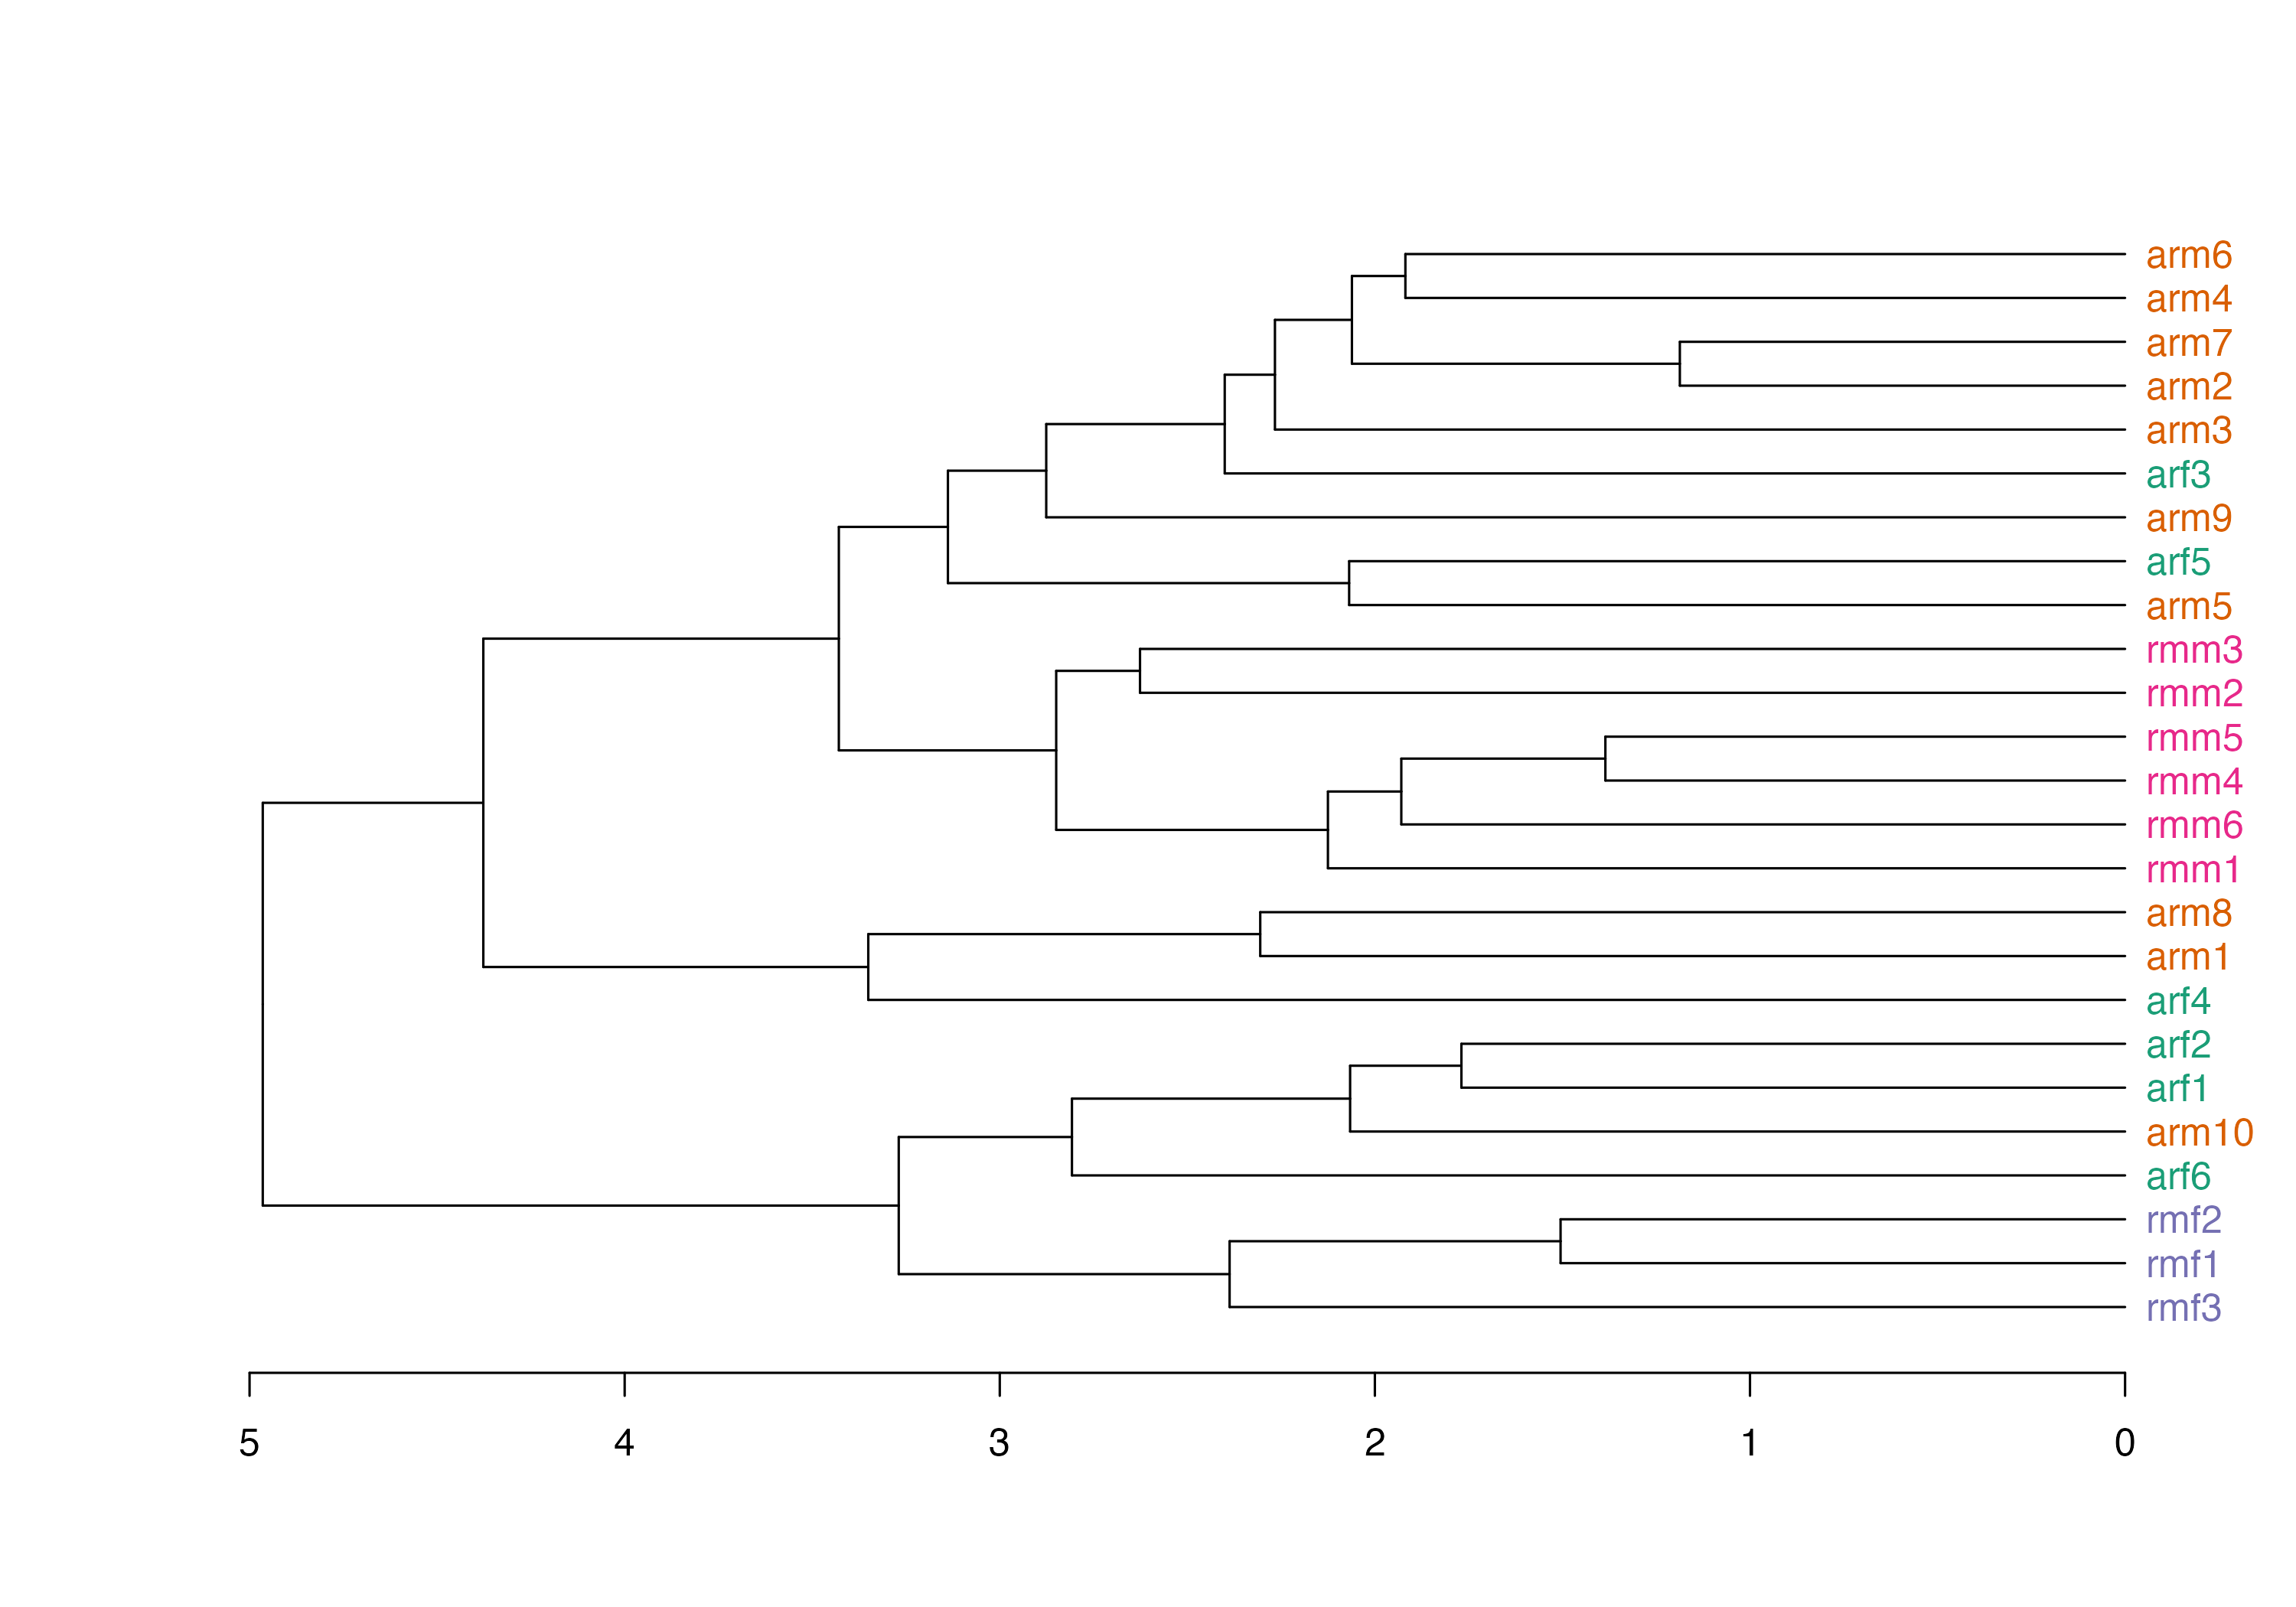
\includegraphics[keepaspectratio]{05_cluster_analysis_files/figure-beamer/unnamed-chunk-12-1.png}}
\end{column}
\end{columns}
\end{frame}

\section{Неиерархические методы
кластеризации}\label{ux43dux435ux438ux435ux440ux430ux440ux445ux438ux447ux435ux441ux43aux438ux435-ux43cux435ux442ux43eux434ux44b-ux43aux43bux430ux441ux442ux435ux440ux438ux437ux430ux446ux438ux438}

\begin{frame}{Метод K-средних (K-means)}
\protect\phantomsection\label{ux43cux435ux442ux43eux434-k-ux441ux440ux435ux434ux43dux438ux445-k-means}
\begin{columns}[T]
\begin{column}{0.5\linewidth}
\pandocbounded{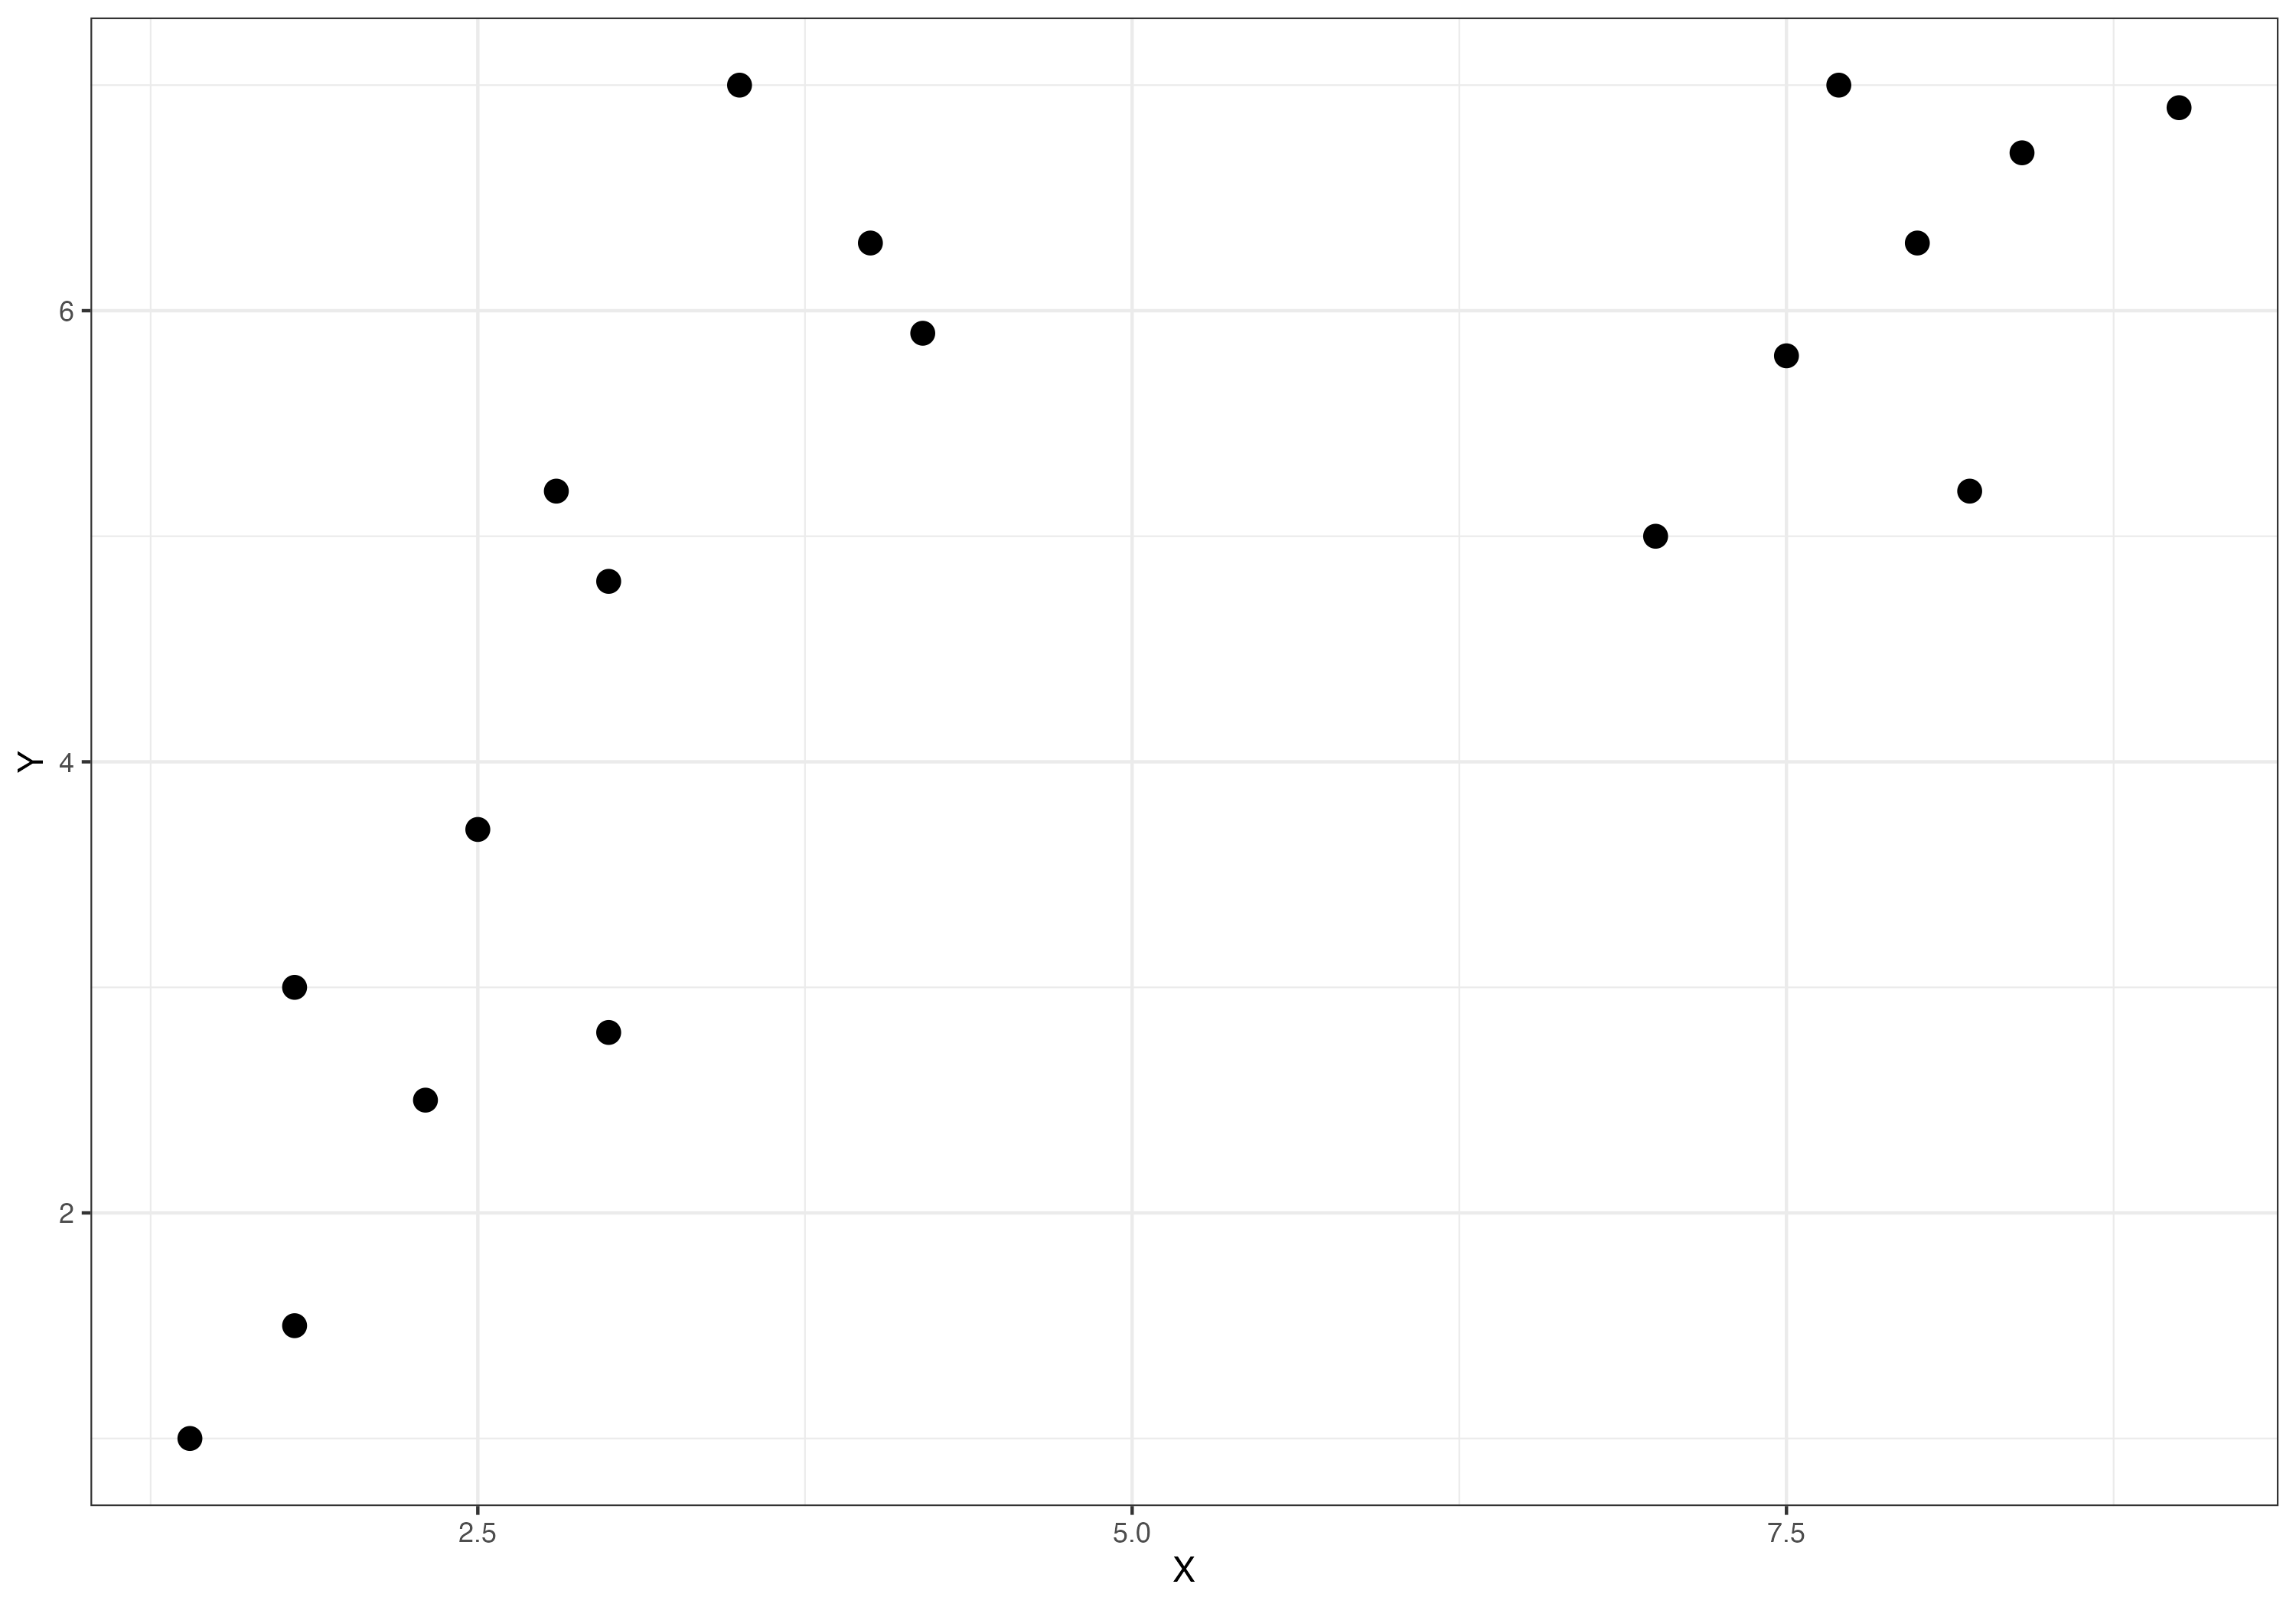
\includegraphics[keepaspectratio]{05_cluster_analysis_files/figure-beamer/unnamed-chunk-13-1.png}}
\end{column}

\begin{column}{0.5\linewidth}
В отличие от иерархических методов кластеризации K-means будет искать то
количество кластеров (k), которое вы ему зададите. Каждое наблюдение
принадлежит кластеру с ближайшим значением среднего числа (центроида);
помимо этого K-means кластеризация минимизирует разброс значений внутри
каждого из кластера.

Используется в машинном обучении, в том числе, например, для цветовой
редуцкии изображений.
\end{column}
\end{columns}
\end{frame}

\begin{frame}{Алгоритм K-means}
\protect\phantomsection\label{ux430ux43bux433ux43eux440ux438ux442ux43c-k-means}
\begin{columns}[T]
\begin{column}{0.5\linewidth}
\textbf{График наблюдений}

\pandocbounded{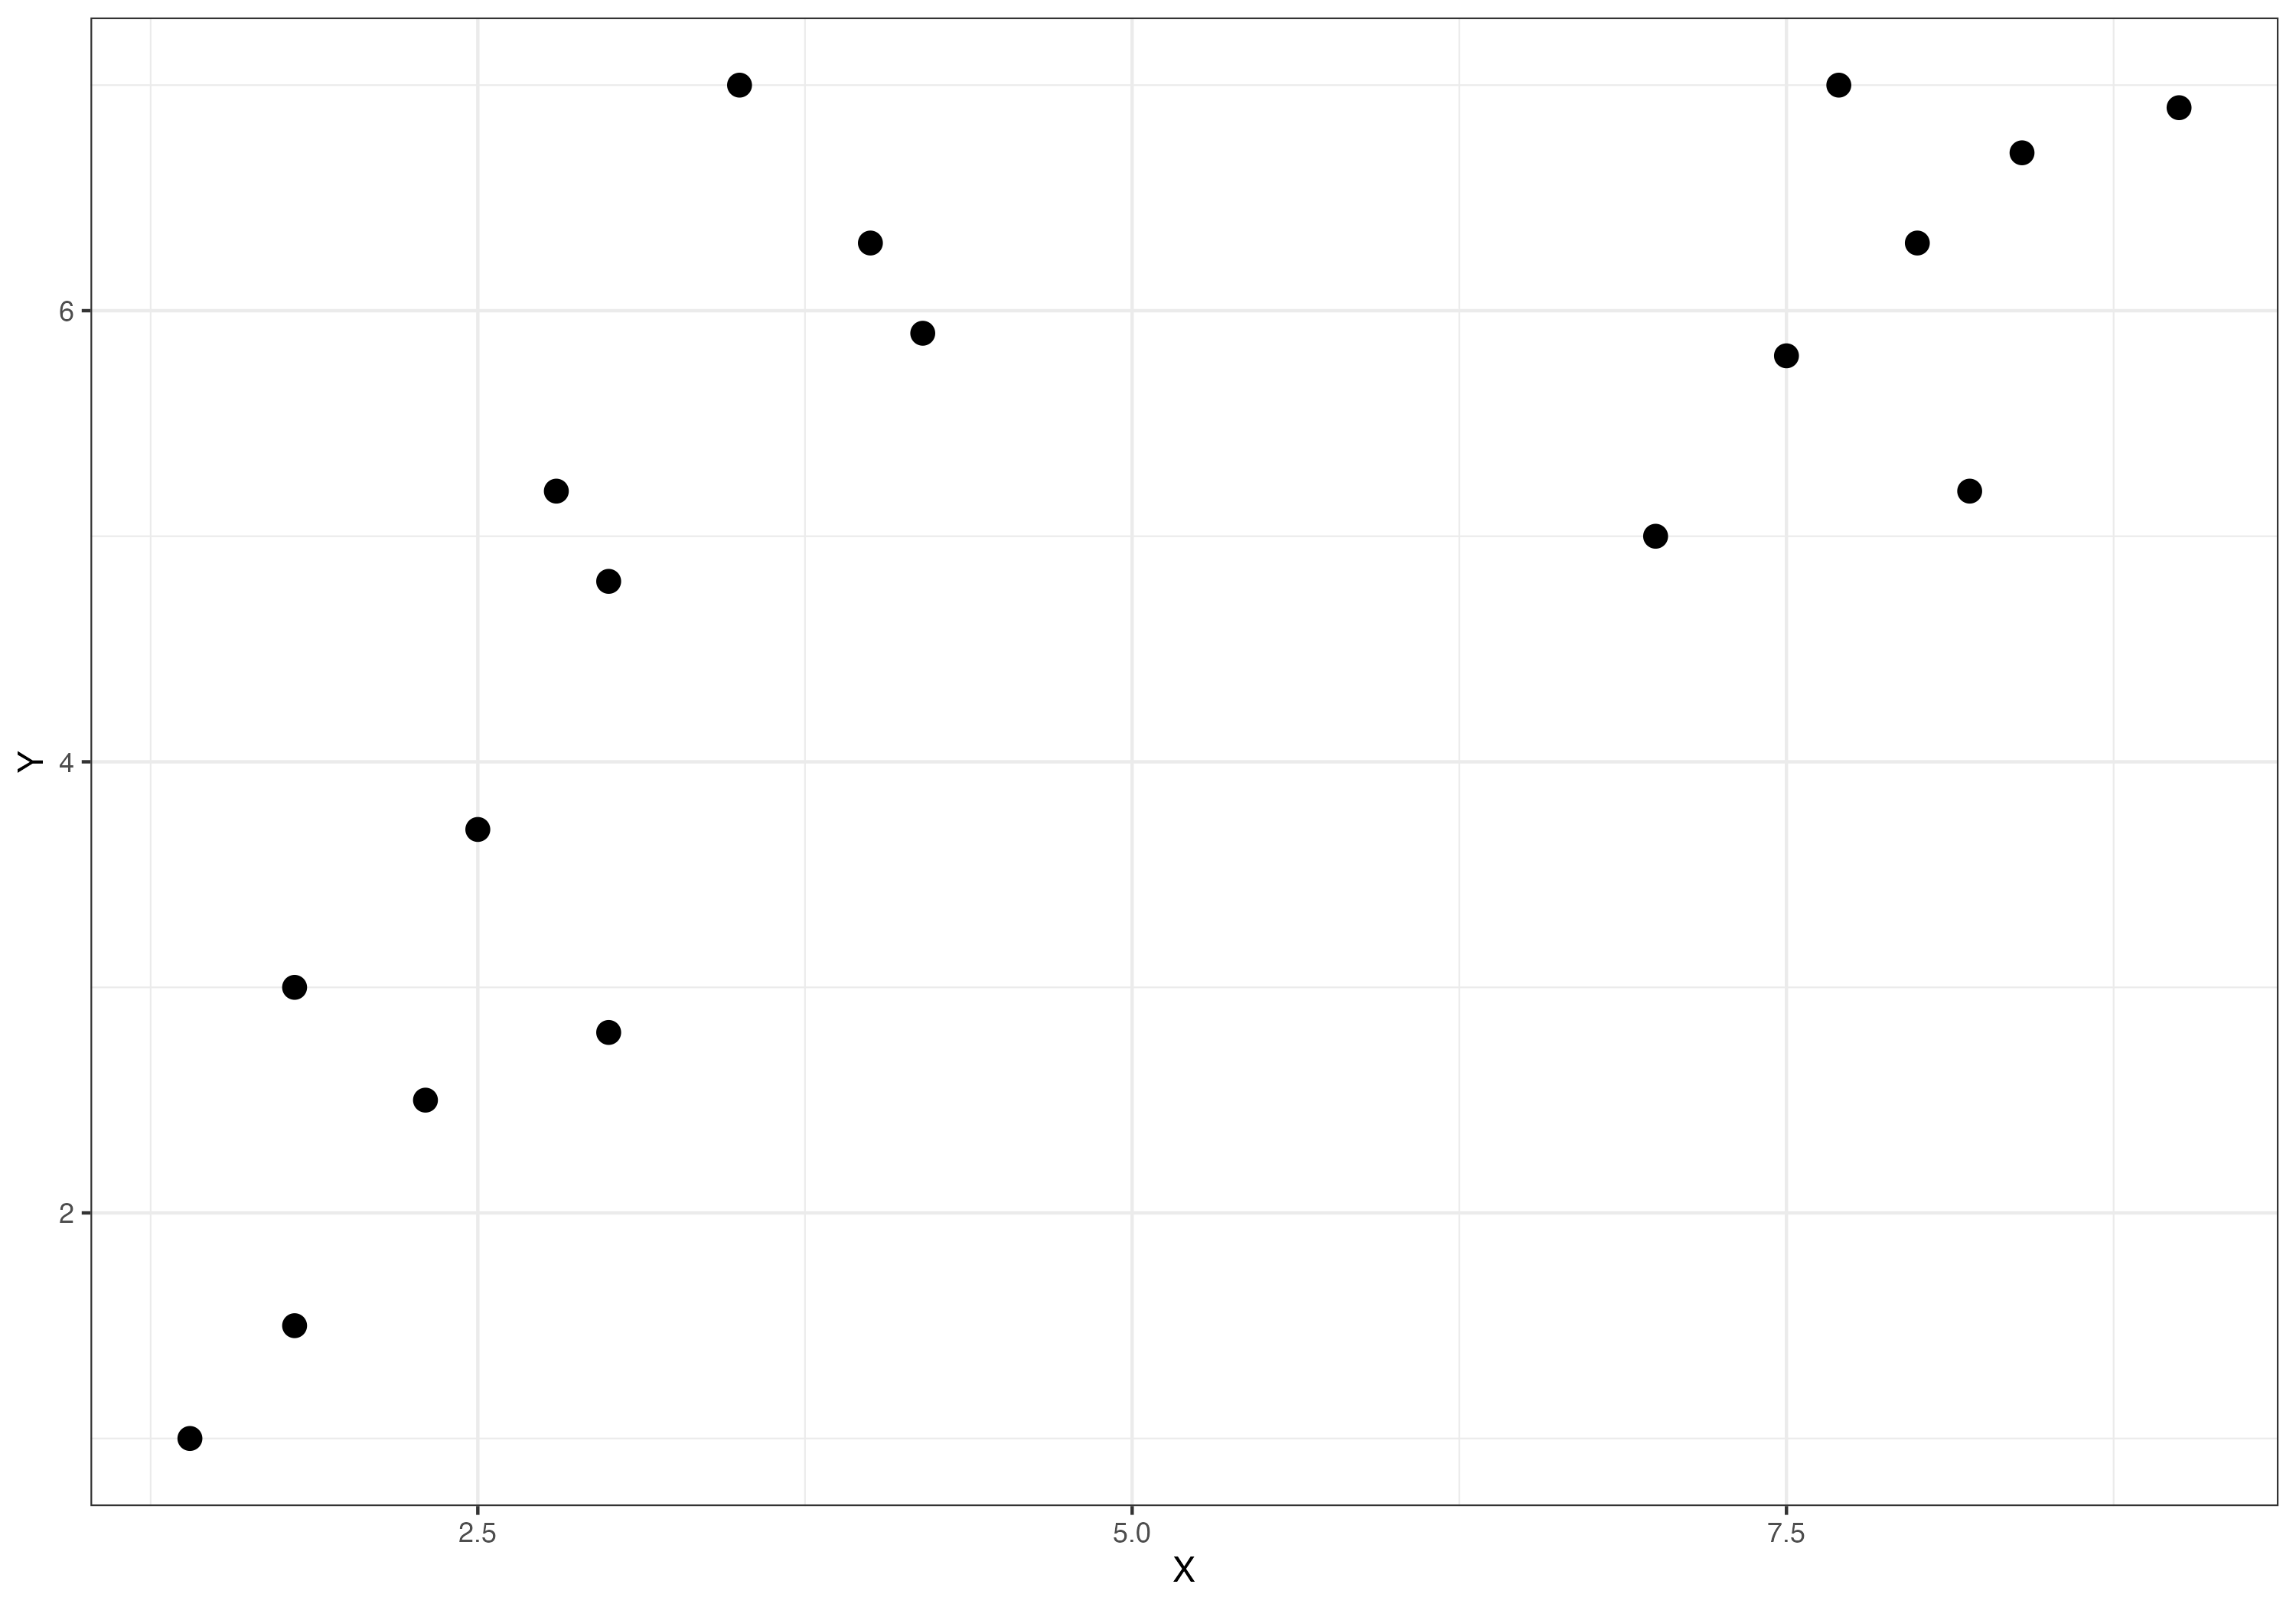
\includegraphics[keepaspectratio]{05_cluster_analysis_files/figure-beamer/unnamed-chunk-14-1.png}}

Здесь как будто бы выделяются 3 кластера, поэтому возьмём k = 3. Что же
будет делать алгоритм?
\end{column}
\end{columns}
\end{frame}

\begin{frame}{Алгоритм K-means}
\protect\phantomsection\label{ux430ux43bux433ux43eux440ux438ux442ux43c-k-means-1}
\begin{columns}[T]
\begin{column}{0.5\linewidth}
\textbf{График наблюдений}

\pandocbounded{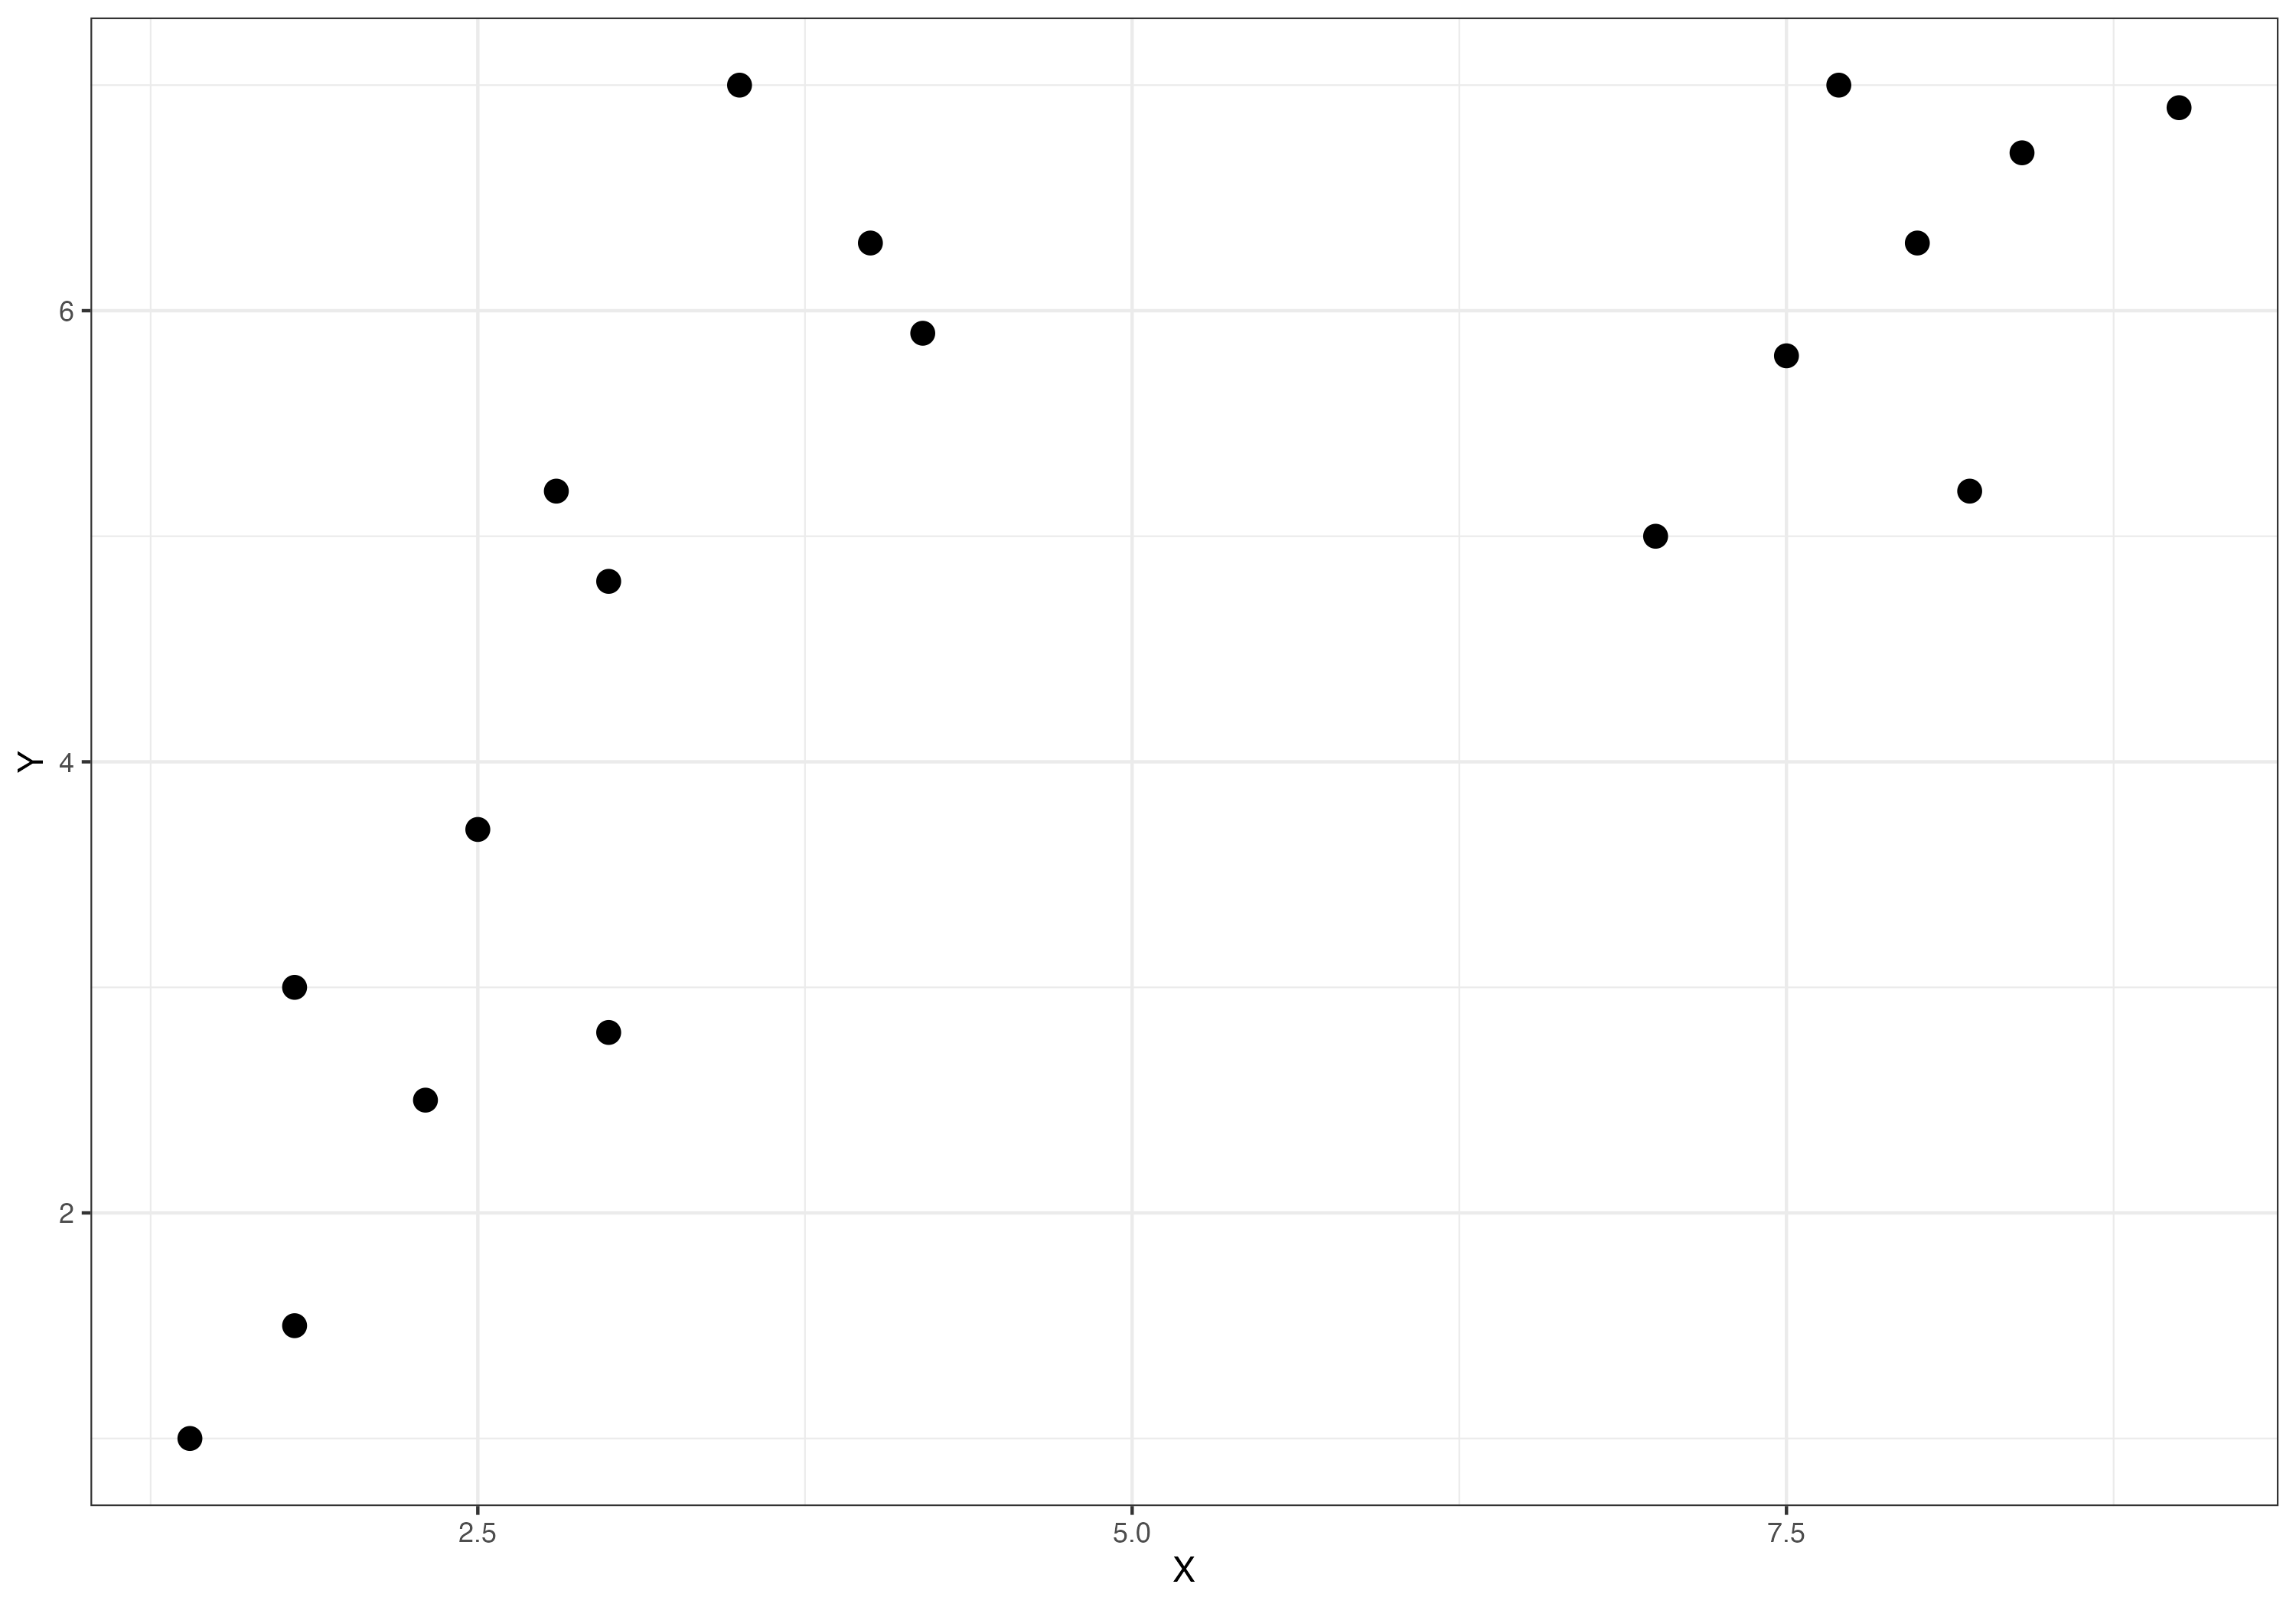
\includegraphics[keepaspectratio]{05_cluster_analysis_files/figure-beamer/unnamed-chunk-15-1.png}}

Здесь как будто бы выделяются 3 кластера, поэтому возьмём k = 3. Что же
будет делать алгоритм?
\end{column}

\begin{column}{0.5\linewidth}
\textbf{1. Выбираются случайным образом 3 точки на графике ---
кластерные центроиды}

Например, так:

\pandocbounded{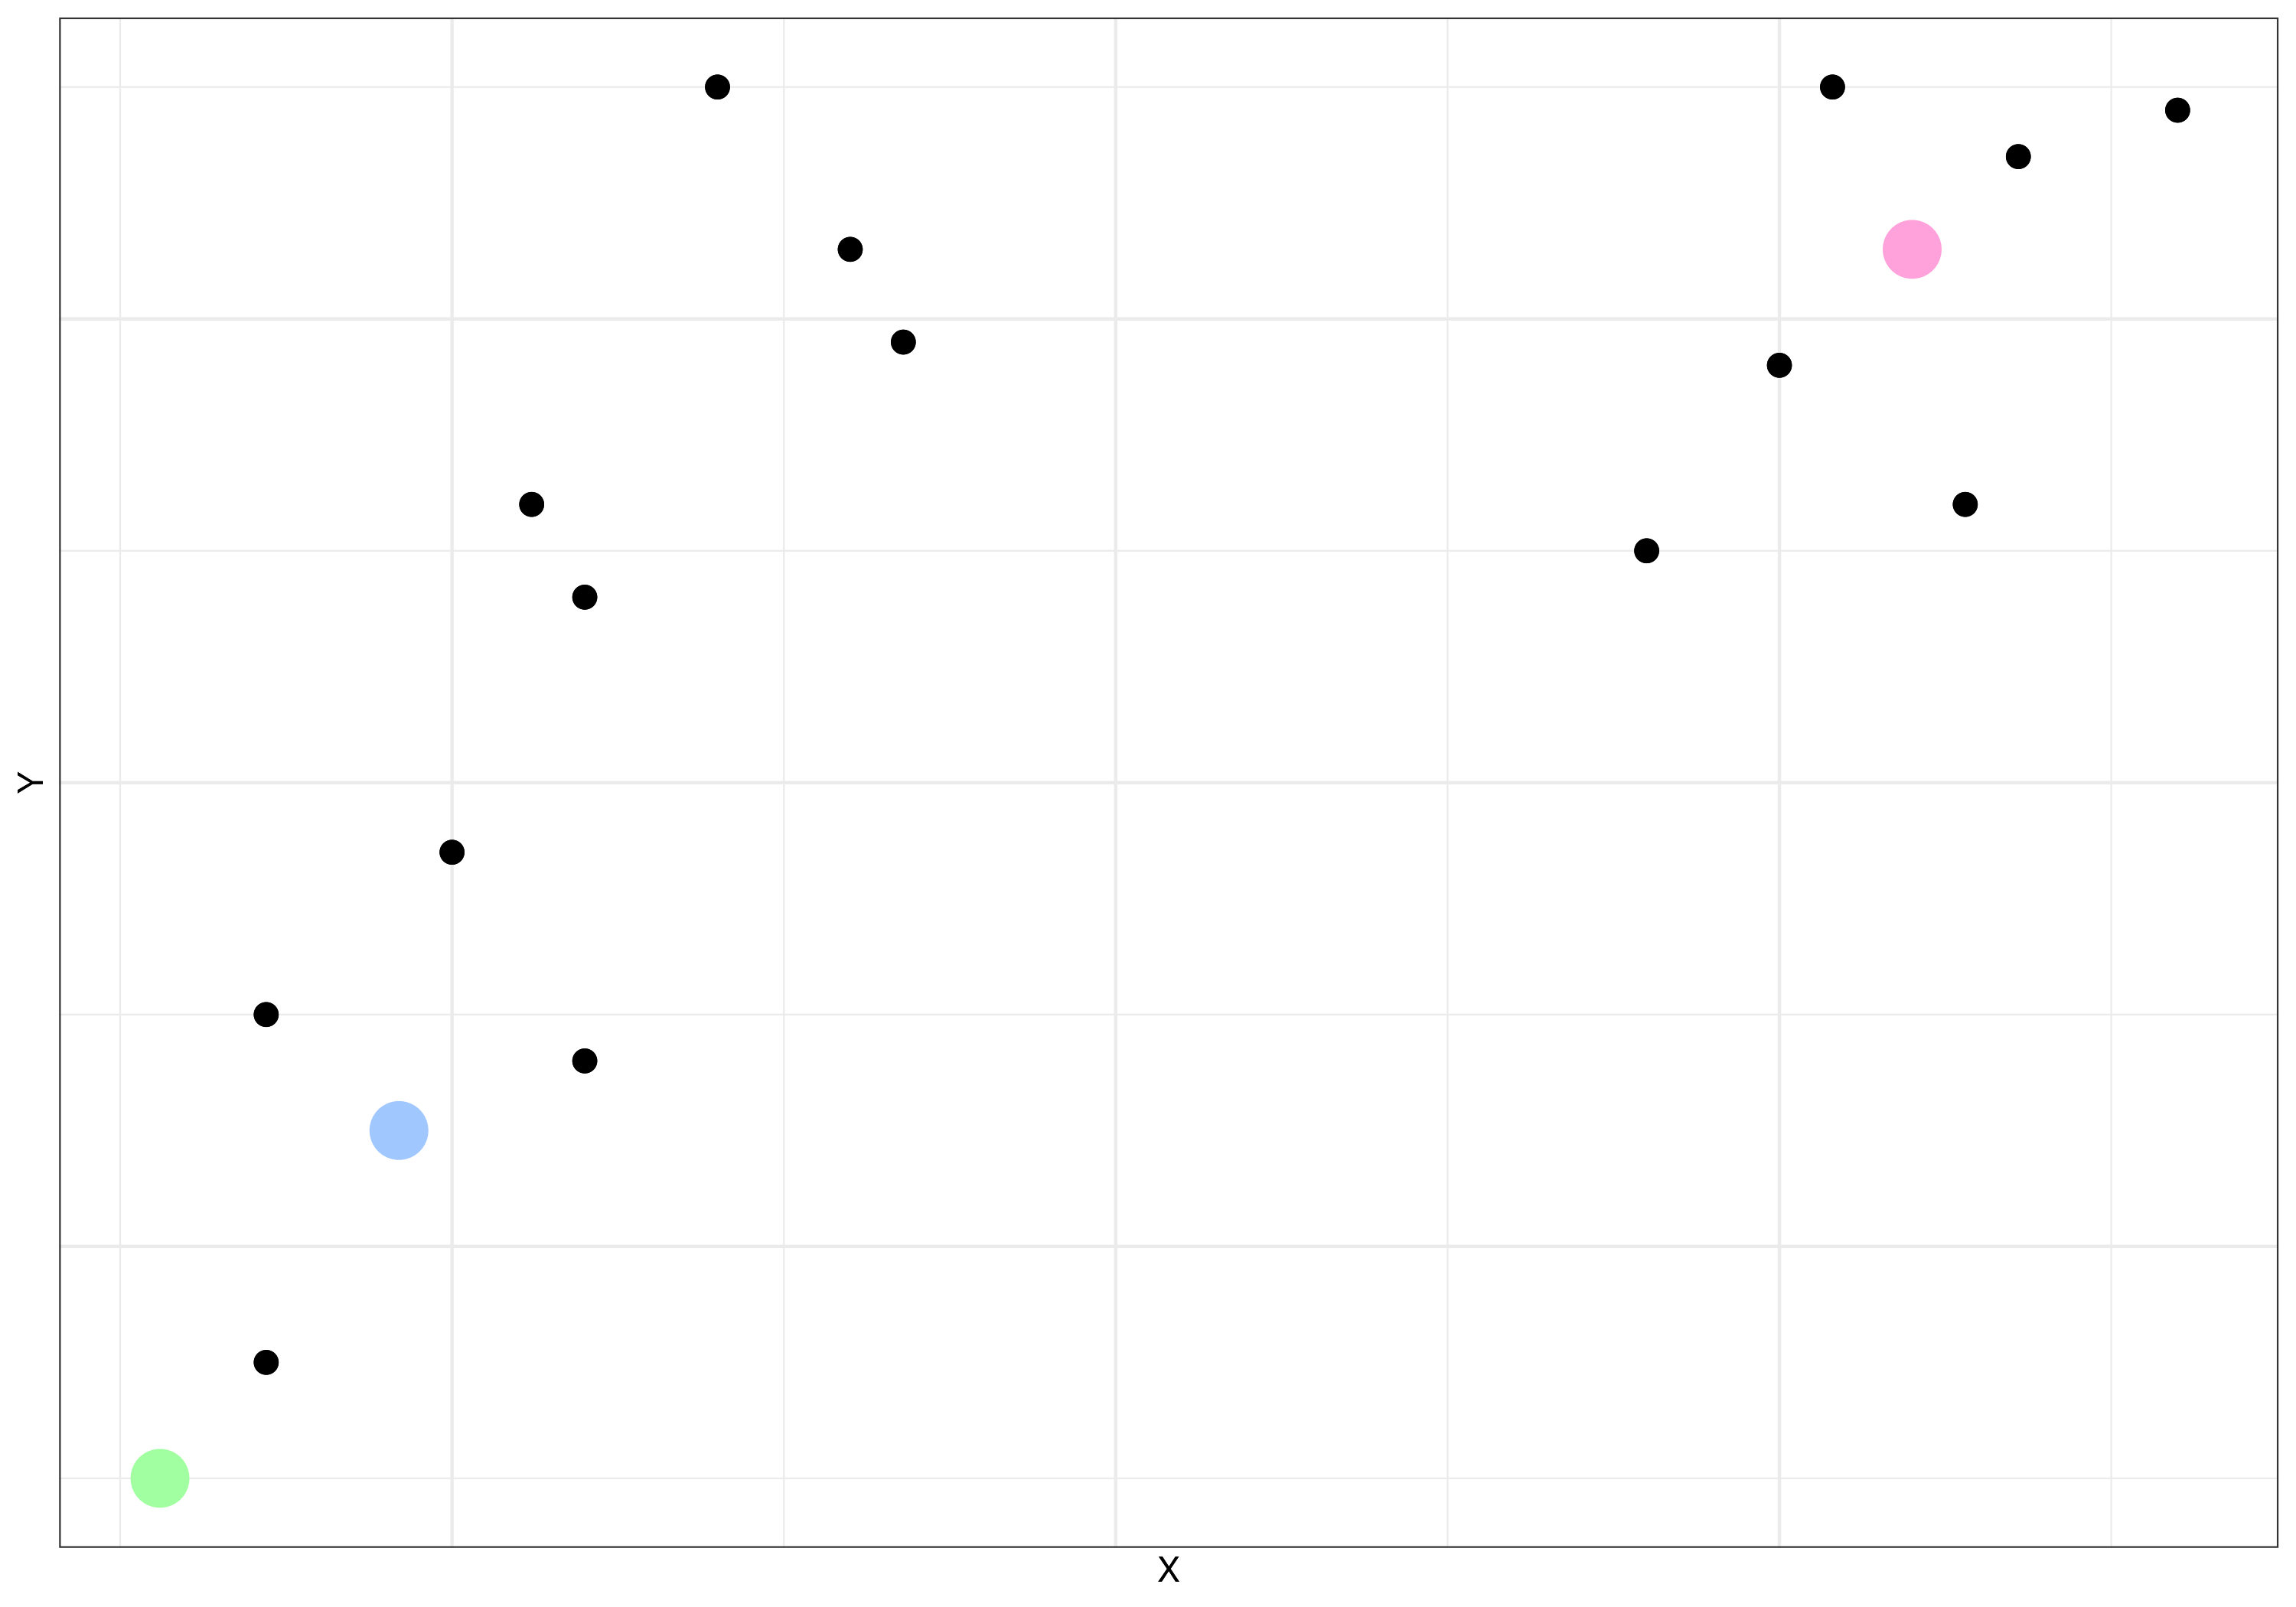
\includegraphics[keepaspectratio]{05_cluster_analysis_files/figure-beamer/unnamed-chunk-16-1.png}}
\end{column}
\end{columns}
\end{frame}

\begin{frame}{Алгоритм K-means}
\protect\phantomsection\label{ux430ux43bux433ux43eux440ux438ux442ux43c-k-means-2}
\begin{columns}[T]
\begin{column}{0.5\linewidth}
\textbf{2. Измеряется Евклидово расстояние между каждой точкой и
центроидом}

При этом каждая точка приписывается к ближайшему кластеру.

\pandocbounded{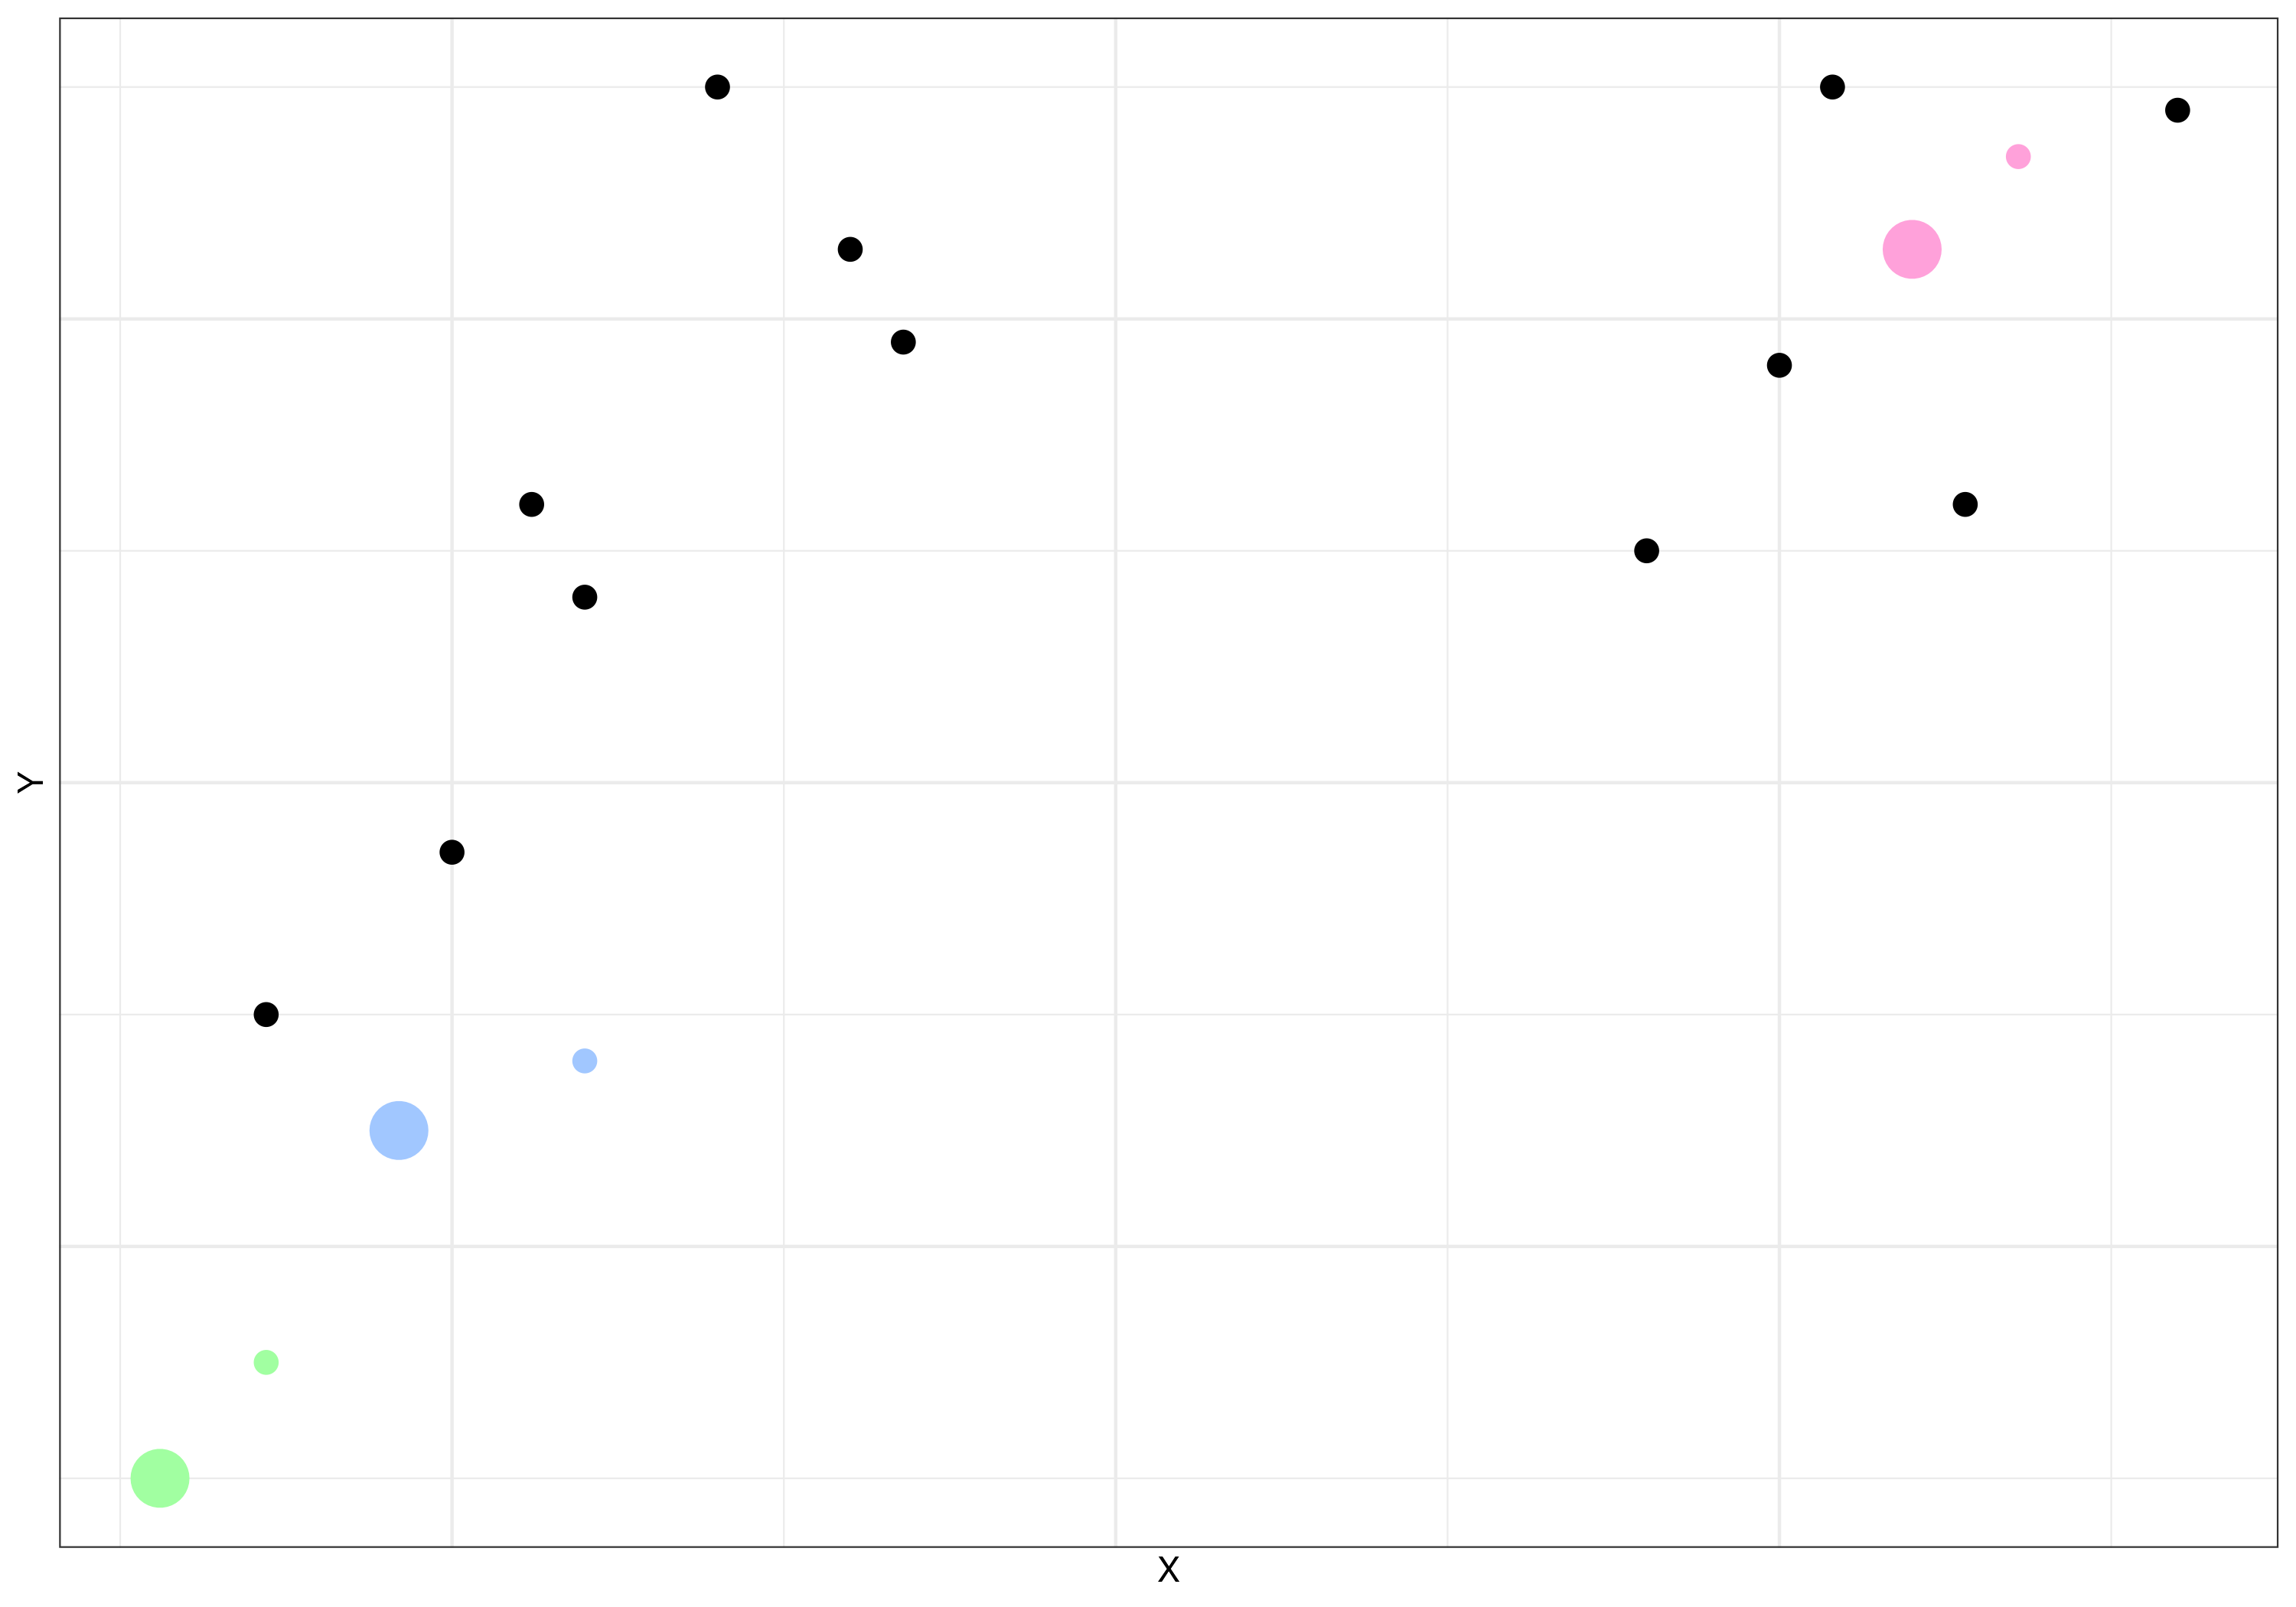
\includegraphics[keepaspectratio]{05_cluster_analysis_files/figure-beamer/unnamed-chunk-17-1.png}}
\end{column}

\begin{column}{0.5\linewidth}
\textbf{3. Расситываются центроиды для каждого кластера}

\pandocbounded{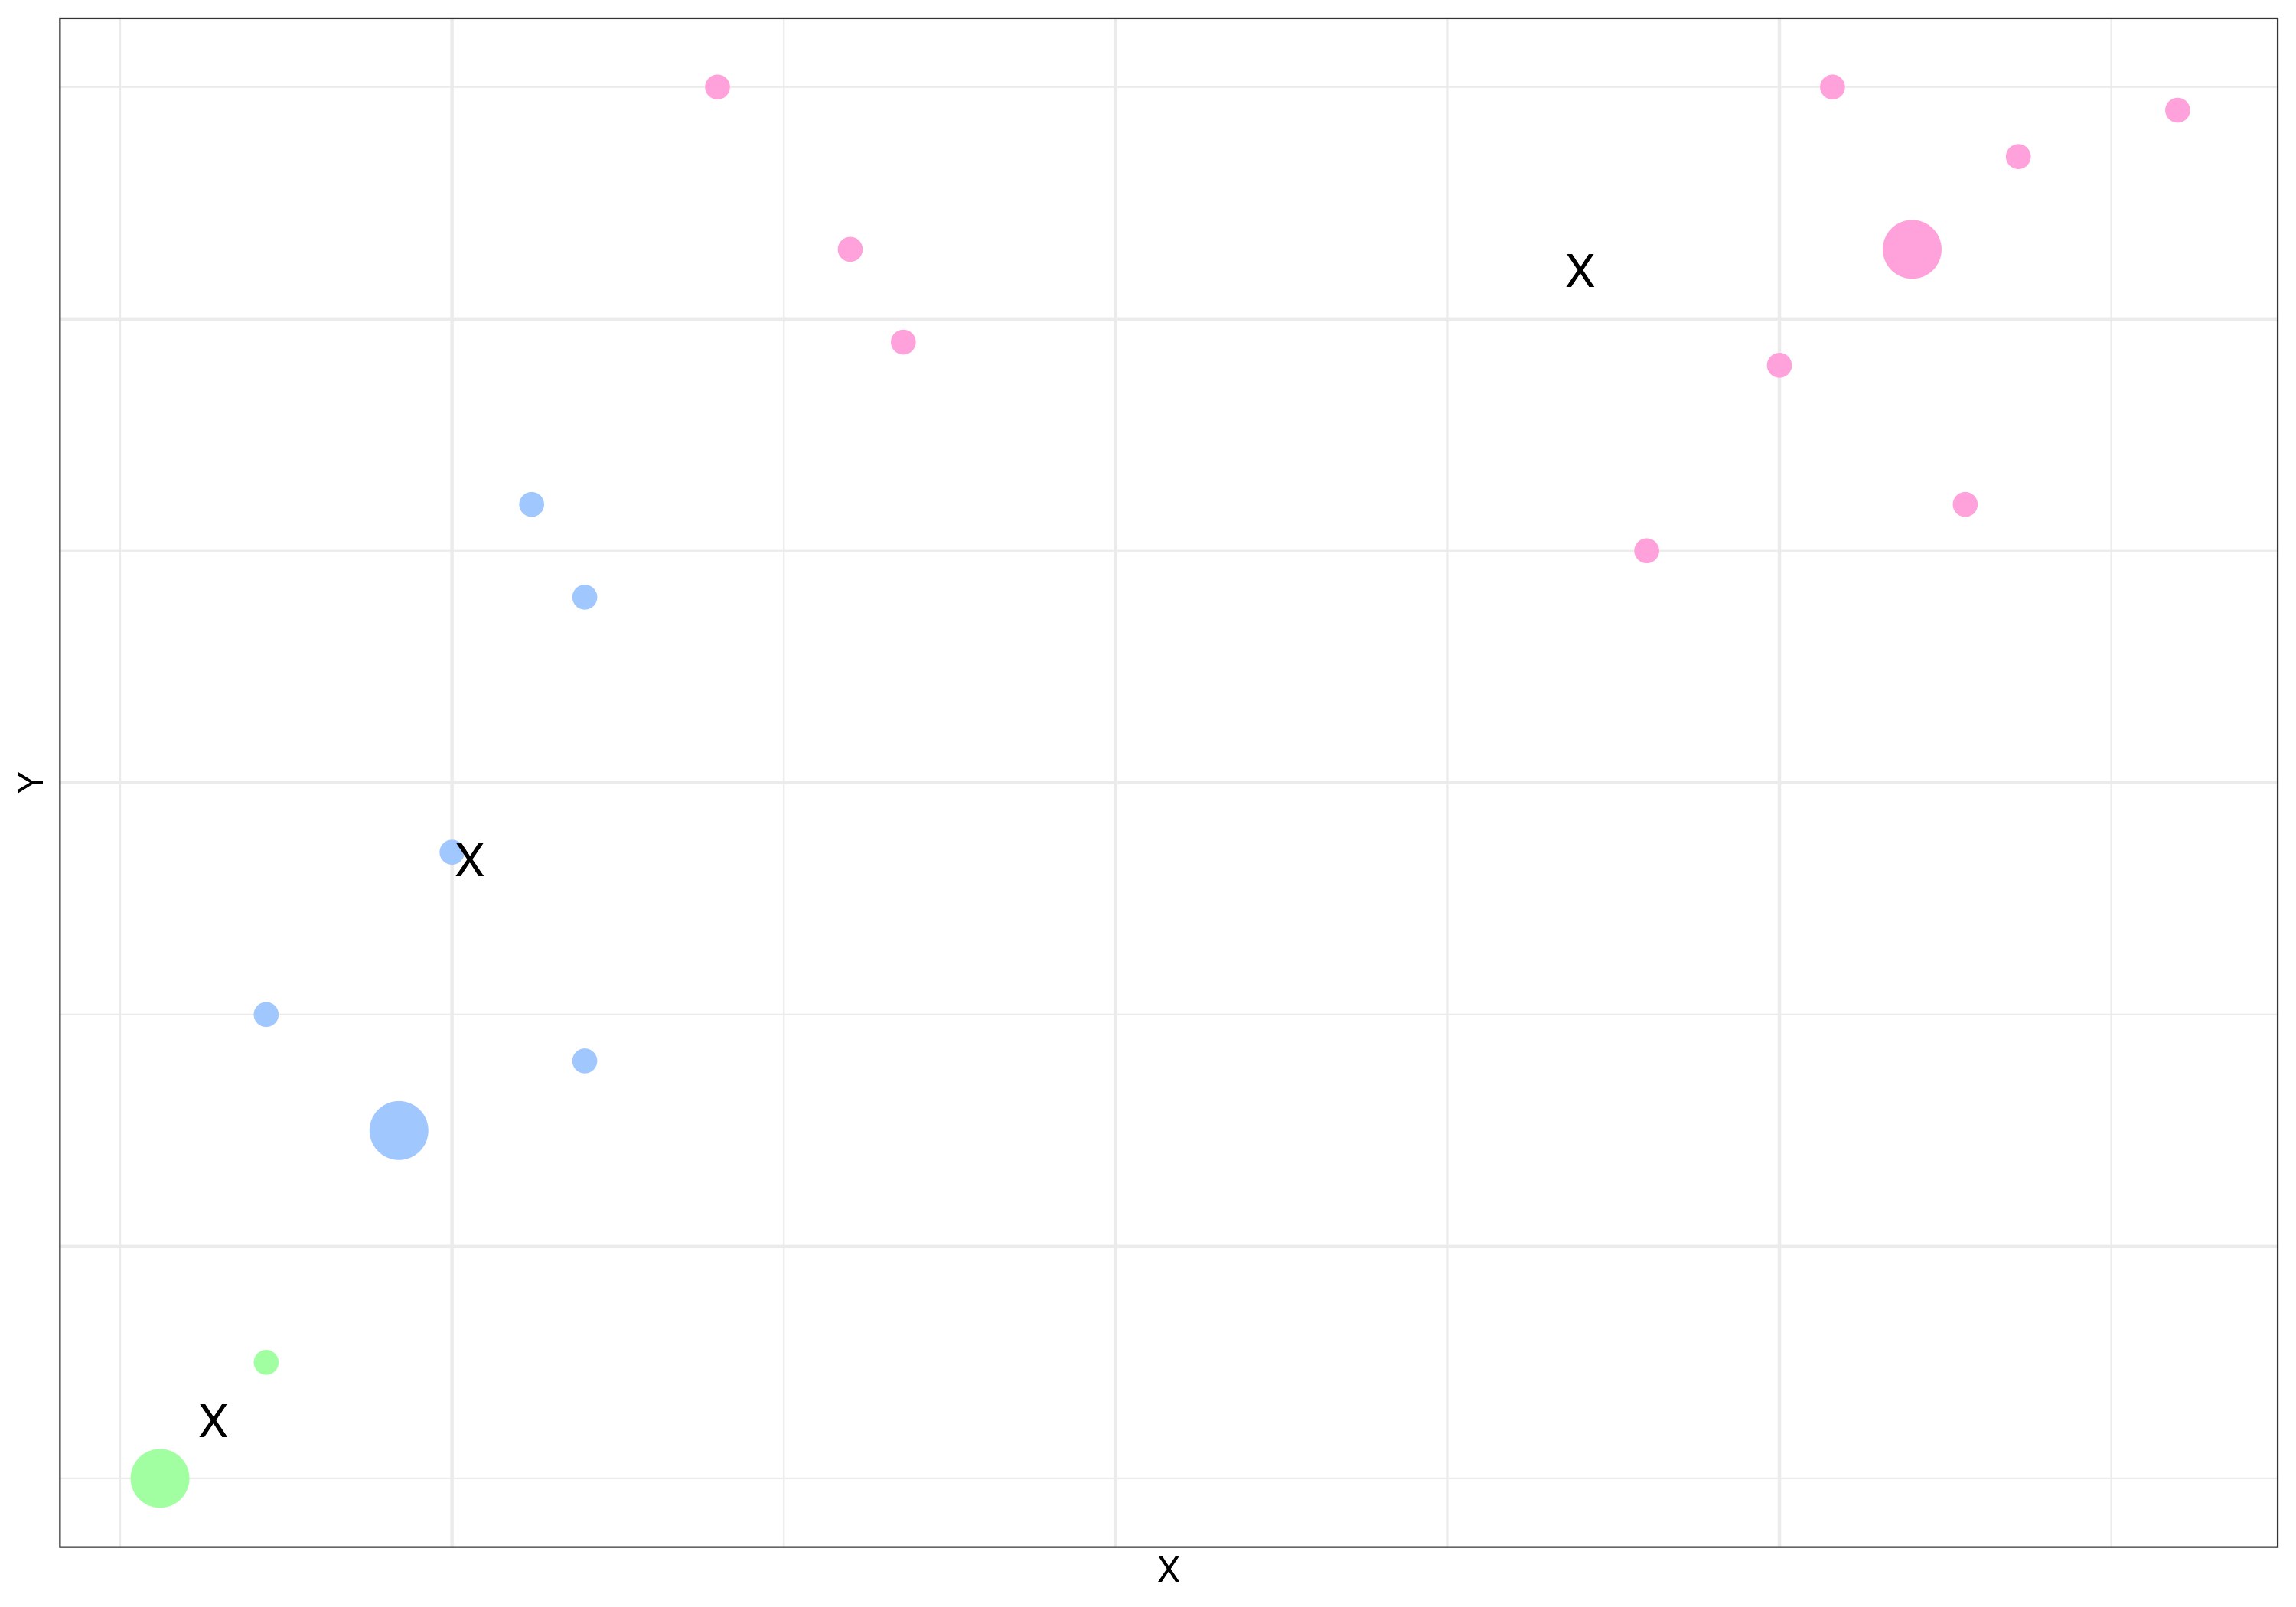
\includegraphics[keepaspectratio]{05_cluster_analysis_files/figure-beamer/unnamed-chunk-18-1.png}}
\end{column}
\end{columns}
\end{frame}

\begin{frame}{4. Расчёт расстояний от каждой точки до нового центроида}
\protect\phantomsection\label{ux440ux430ux441ux447ux451ux442-ux440ux430ux441ux441ux442ux43eux44fux43dux438ux439-ux43eux442-ux43aux430ux436ux434ux43eux439-ux442ux43eux447ux43aux438-ux434ux43e-ux43dux43eux432ux43eux433ux43e-ux446ux435ux43dux442ux440ux43eux438ux434ux430}
\begin{columns}[T]
\begin{column}{0.5\linewidth}
Также оценивается разброс внутри каждого кластера.

\pandocbounded{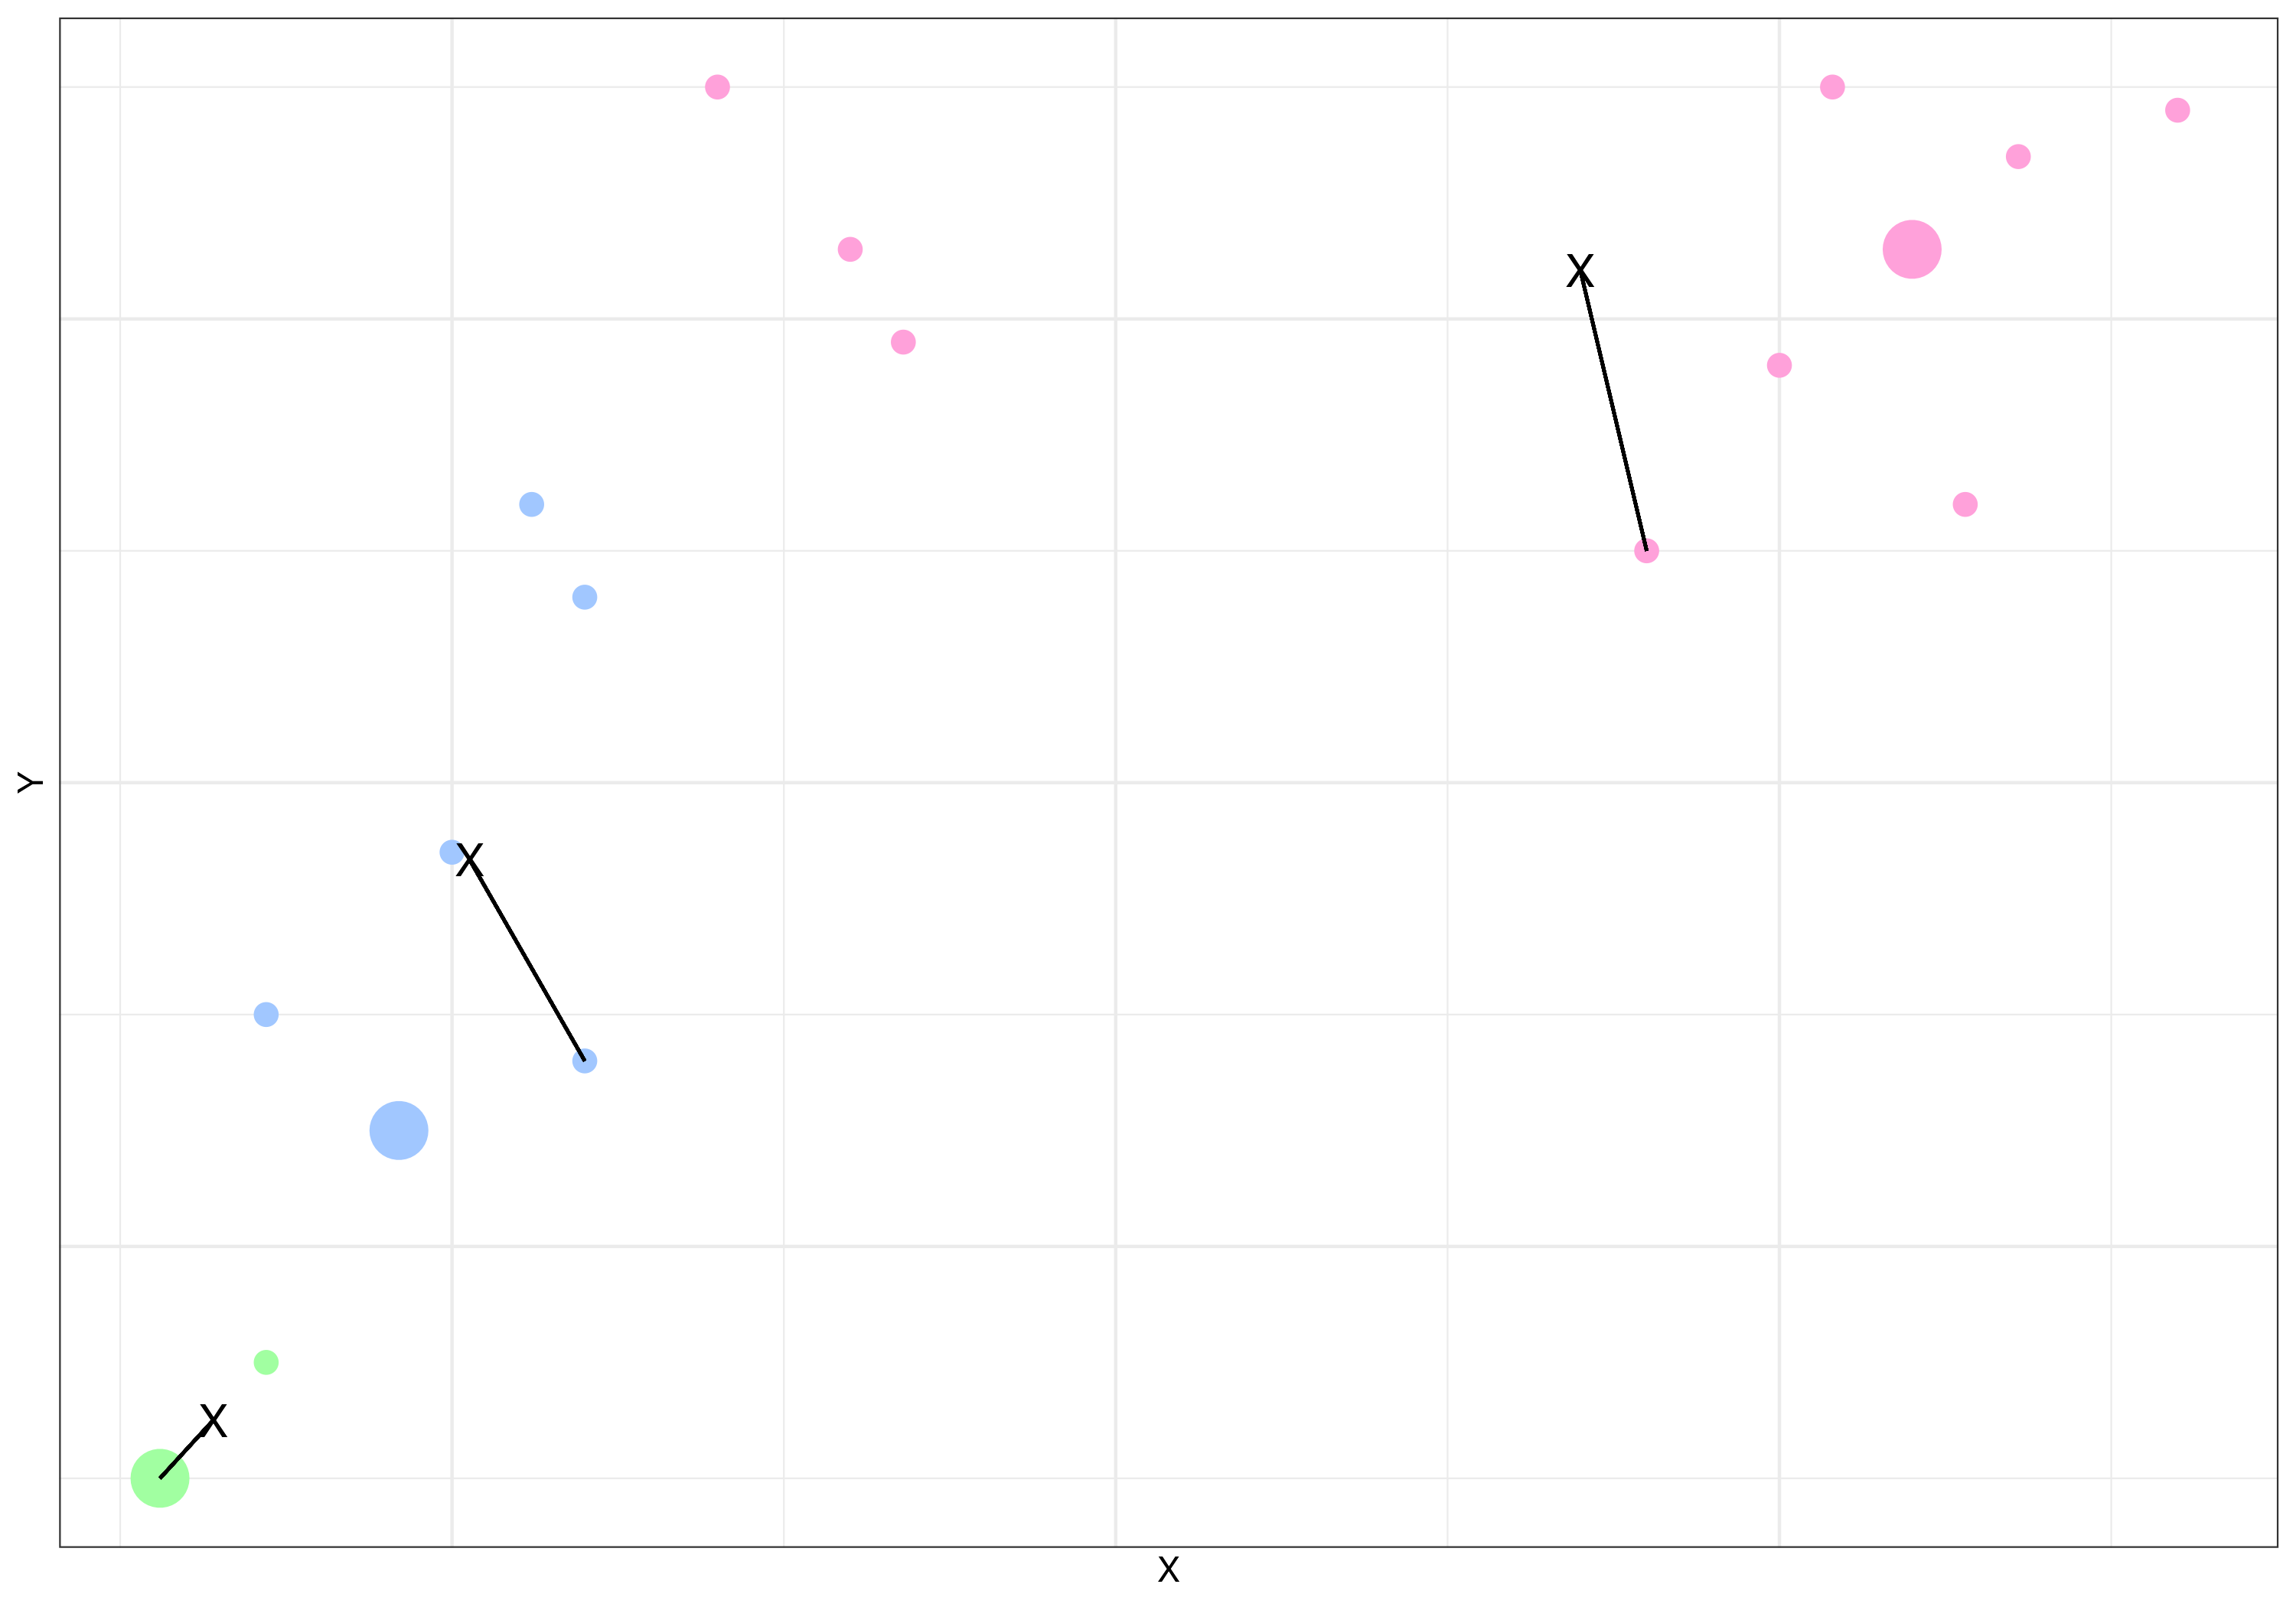
\includegraphics[keepaspectratio]{05_cluster_analysis_files/figure-beamer/unnamed-chunk-19-1.png}}
\end{column}

\begin{column}{0.5\linewidth}
Разброс считается как сумма квадратов расстояний между отдельными
наблюдениями и центроидом.

\[ \sum_{i=1}^{n}(x_i - \overline{x})\]
\end{column}
\end{columns}
\end{frame}

\begin{frame}{5. Повторяем всё многократно до тех пор, пока разброс не
станет минимальным}
\protect\phantomsection\label{ux43fux43eux432ux442ux43eux440ux44fux435ux43c-ux432ux441ux451-ux43cux43dux43eux433ux43eux43aux440ux430ux442ux43dux43e-ux434ux43e-ux442ux435ux445-ux43fux43eux440-ux43fux43eux43aux430-ux440ux430ux437ux431ux440ux43eux441-ux43dux435-ux441ux442ux430ux43dux435ux442-ux43cux438ux43dux438ux43cux430ux43bux44cux43dux44bux43c}
Кластеры с минимальным разбросом --- финальные.

\pandocbounded{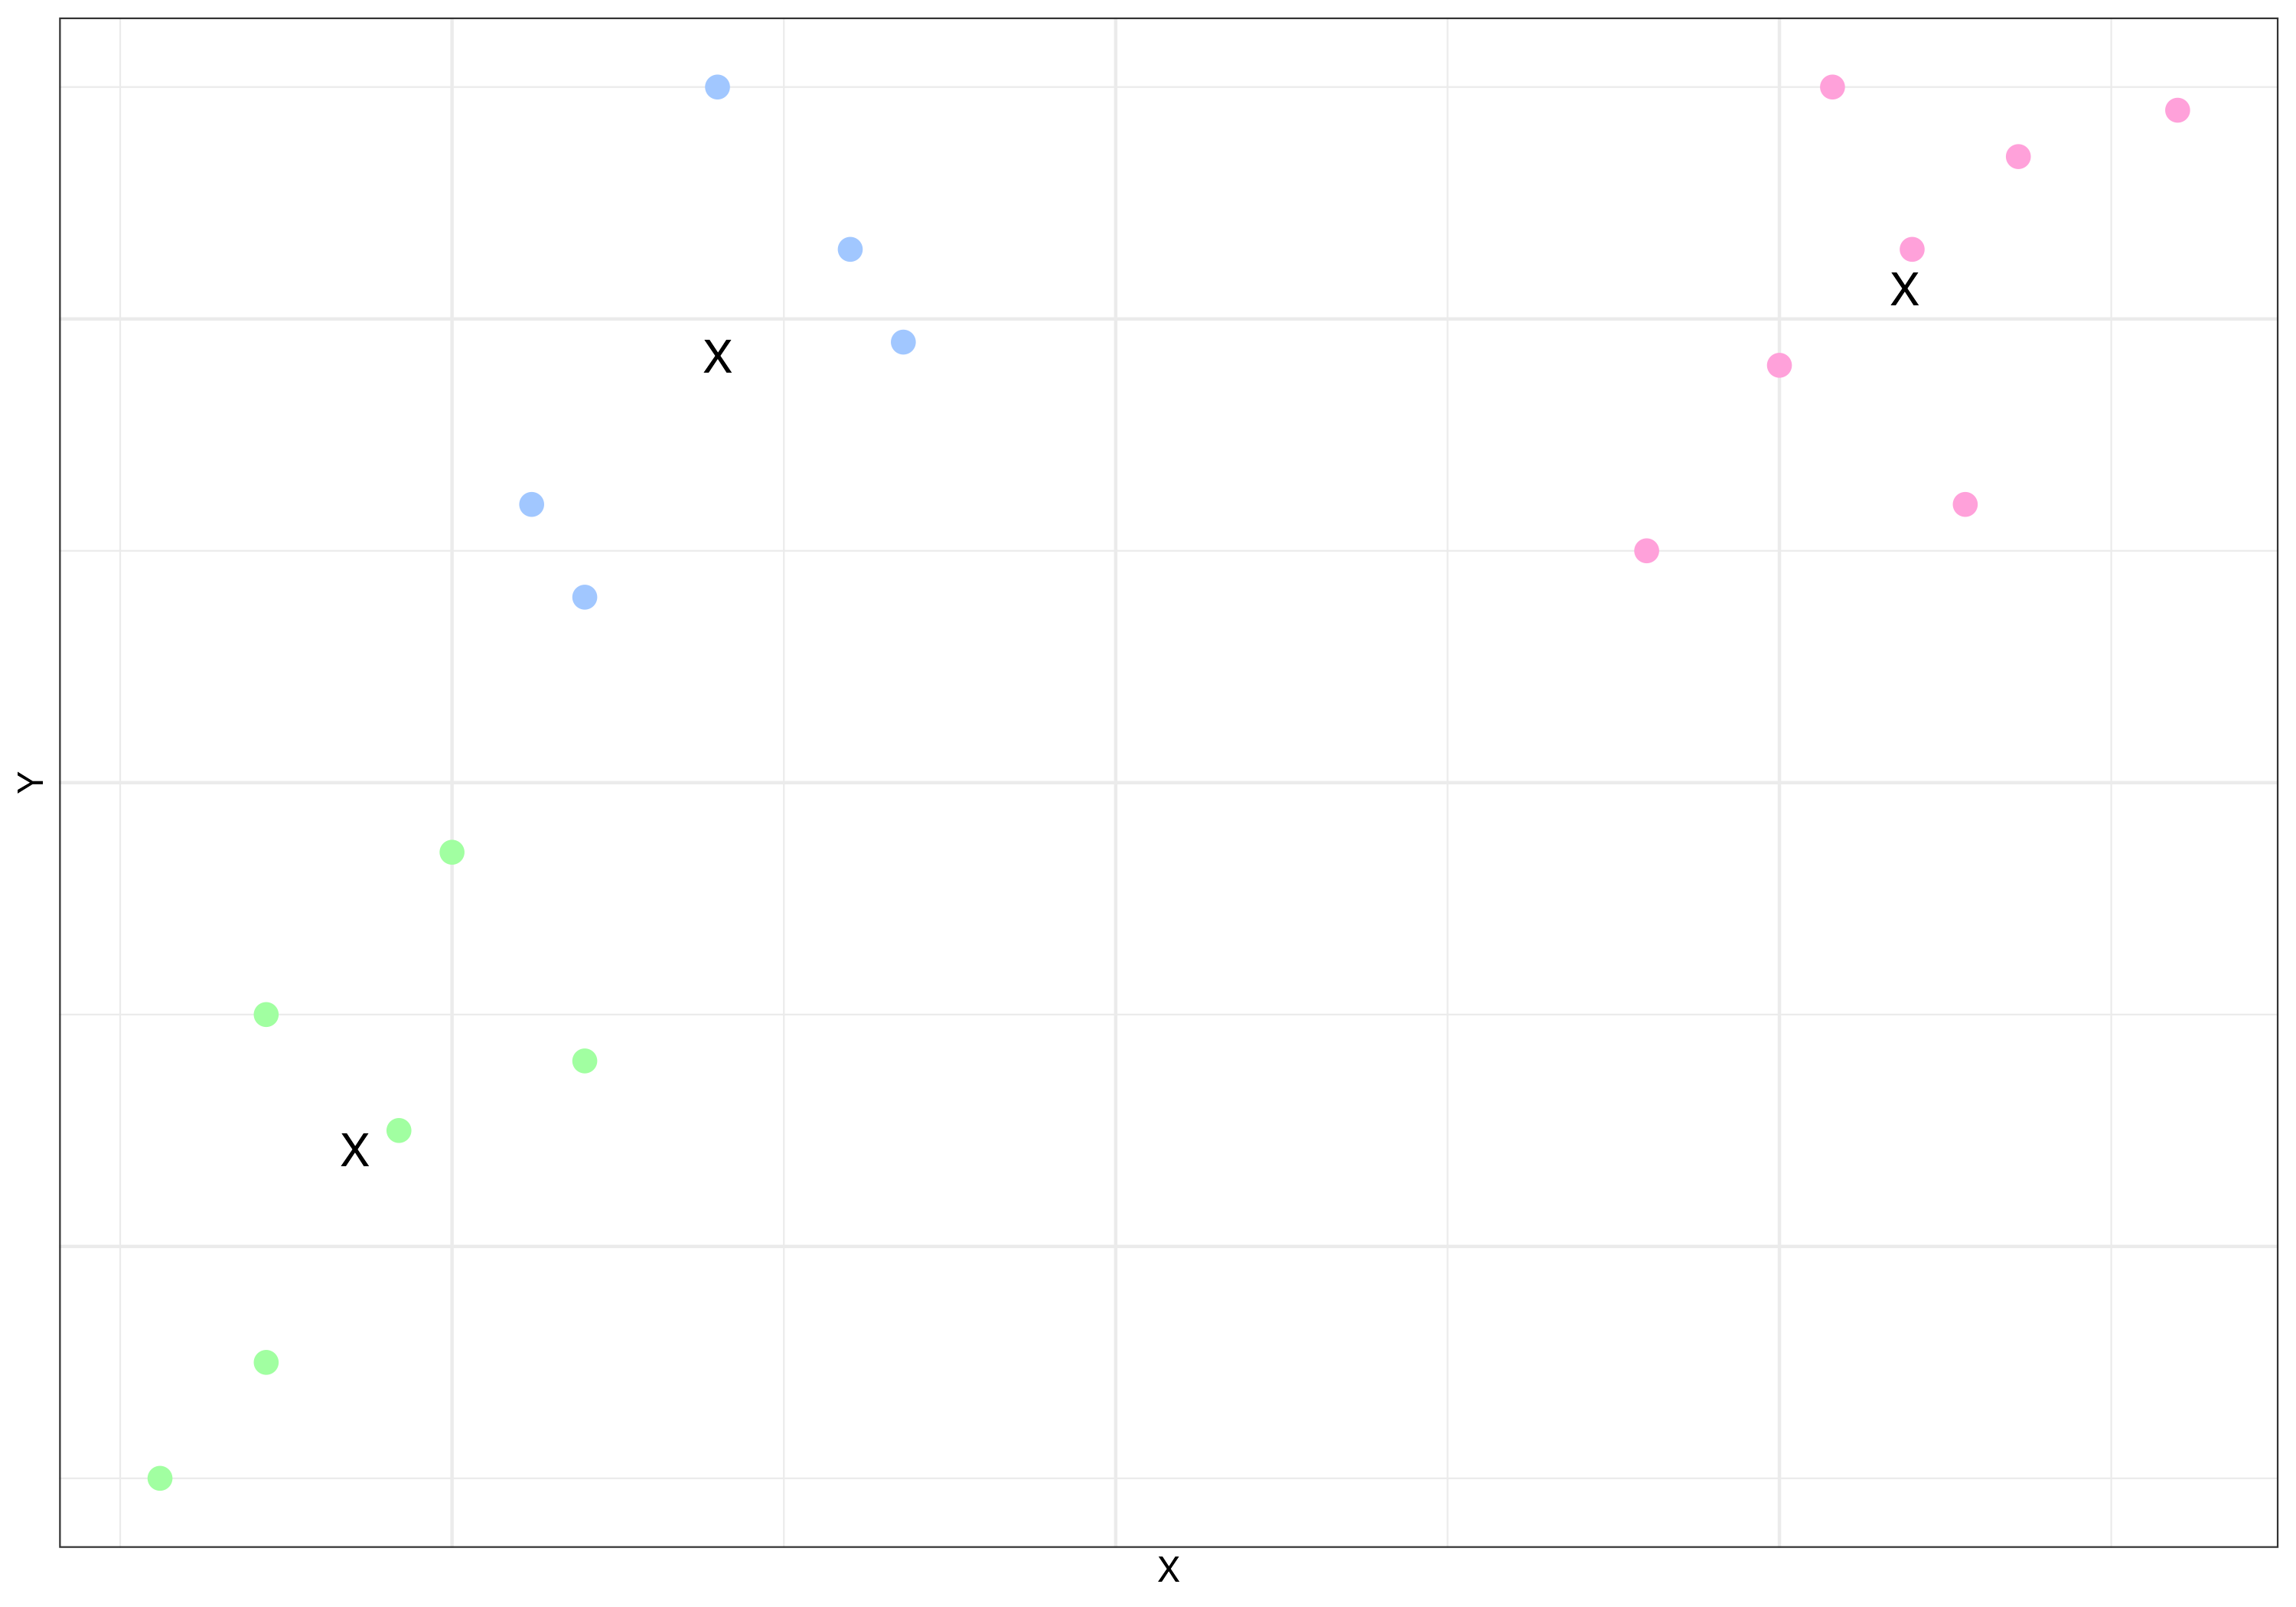
\includegraphics[keepaspectratio]{05_cluster_analysis_files/figure-beamer/unnamed-chunk-20-1.png}}
\end{frame}

\begin{frame}{Поиск локального минимума}
\protect\phantomsection\label{ux43fux43eux438ux441ux43a-ux43bux43eux43aux430ux43bux44cux43dux43eux433ux43e-ux43cux438ux43dux438ux43cux443ux43cux430}
\centering

\includegraphics[width=0.55\linewidth,height=\textheight,keepaspectratio]{images/kmeans_algorithm_local.png}

\raggedright

Из Legendre, Legendre, 2012

Кратко алгоритм можно свести к поиску общего минимума среди локальных
(вне зависимости от начальной конфигурации).
\end{frame}

\begin{frame}[fragile]{K-means в R}
\protect\phantomsection\label{k-means-ux432-r}
Если в данных много нулей, их обязательно нужно стандартизовать (что мы
уже делали).

K-means кластеризацию в R делает функция \texttt{kmeans} (пакет
\texttt{stats}), ей нужно передать аргументы \texttt{centers}
(количество кластеров) и \texttt{nstart} (количество случайных
итераций).

\begin{Shaded}
\begin{Highlighting}[]
\FunctionTok{set.seed}\NormalTok{(}\DecValTok{333}\NormalTok{)}
\NormalTok{w\_kmeans }\OtherTok{\textless{}{-}} \FunctionTok{kmeans}\NormalTok{(st\_w, }\AttributeTok{centers =} \DecValTok{3}\NormalTok{, }\AttributeTok{nstart =} \DecValTok{100}\NormalTok{)}
\end{Highlighting}
\end{Shaded}

Полученные результаты можно сравнить с тем, что нам дала иерархическая
кластеризация (UPGMA) --- оценка ширины силуэта.

\begin{Shaded}
\begin{Highlighting}[]
\FunctionTok{table}\NormalTok{(avg3, w\_kmeans}\SpecialCharTok{$}\NormalTok{cluster)}
\end{Highlighting}
\end{Shaded}

\begin{verbatim}
    
avg3 1 2 3
   1 6 0 9
   2 0 7 0
   3 0 1 2
\end{verbatim}
\end{frame}

\begin{frame}{Как выбрать нужное количество кластеров?}
\protect\phantomsection\label{ux43aux430ux43a-ux432ux44bux431ux440ux430ux442ux44c-ux43dux443ux436ux43dux43eux435-ux43aux43eux43bux438ux447ux435ux441ux442ux432ux43e-ux43aux43bux430ux441ux442ux435ux440ux43eux432}
Два популярных критерия:

\begin{itemize}
\item
  Индекс Калински-Харабаза (Calinski--Harabasz index): F-статистика,
  сравнивающая меж- и внутригрупповую сумму квадратов. Если группы
  одинаковой величины.
\item
  Индекс простой структуры (Simple Structure Index): оценивает влияние
  на интепретабельность полученной кластеризации. Если группы разной
  величины.
\end{itemize}
\end{frame}

\begin{frame}{Критерии выбора количества кластеров}
\protect\phantomsection\label{ux43aux440ux438ux442ux435ux440ux438ux438-ux432ux44bux431ux43eux440ux430-ux43aux43eux43bux438ux447ux435ux441ux442ux432ux430-ux43aux43bux430ux441ux442ux435ux440ux43eux432}
\begin{columns}[T]
\begin{column}{0.5\linewidth}
\textbf{Индекс Калински-Харабаза}

\[CH(k) = \frac{SS_B / (k-1)}{SS_W / (n-k)}\]

где:

\begin{itemize}
\tightlist
\item
  \(SS_B\) --- сумма квадратов расстояний от центроида кластера до
  общего центроида, умноженное на количество объектов в кластере,
\item
  \(SS_W\) --- сумма квадратов расстояний до центроида собственного
  кластера,
\item
  \(k\) --- число кластеров,
\item
  \(n\) --- количество исходных наблюдений.
\end{itemize}

Выбирается число кластеров с \textbf{наибольшим} значением CH.
\end{column}

\begin{column}{0.5\linewidth}
\textbf{Индекс простой структуры}

\[SSI = \frac{1}{n}\sum_{i=1}^{n} \frac{b_i - a_i}{\max(a_i, b_i)}\]

где:

\begin{itemize}
\tightlist
\item
  \(a_i\) --- расстояние от объекта \(i\) до центроида своего кластера,
\item
  \(b_i\) --- расстояние от объекта \(i\) до ближайшего центроида
  другого кластера,
\item
  \(n\) --- количество исходных наблюдений по всем кластерам.
\end{itemize}

Выбирается число кластеров с \textbf{наибольшим} значением SSI.
\end{column}
\end{columns}
\end{frame}

\begin{frame}[fragile]{Как выбрать нужное количество кластеров в R}
\protect\phantomsection\label{ux43aux430ux43a-ux432ux44bux431ux440ux430ux442ux44c-ux43dux443ux436ux43dux43eux435-ux43aux43eux43bux438ux447ux435ux441ux442ux432ux43e-ux43aux43bux430ux441ux442ux435ux440ux43eux432-ux432-r}
Функция \texttt{cascadeKM} из пакета \texttt{vegan}. По сути
функция-обёртка, которая проводит кластеризацию с разным заданным
количеством кластеров.

\begin{Shaded}
\begin{Highlighting}[]
\NormalTok{w\_cascade }\OtherTok{\textless{}{-}} \FunctionTok{cascadeKM}\NormalTok{(st\_w, }\AttributeTok{inf.gr =} \DecValTok{2}\NormalTok{, }\AttributeTok{sup.gr =} \DecValTok{10}\NormalTok{, }
                       \AttributeTok{iter =} \DecValTok{100}\NormalTok{, }\AttributeTok{criterion =} \StringTok{\textquotesingle{}calinski\textquotesingle{}}\NormalTok{)}
\end{Highlighting}
\end{Shaded}

\begin{itemize}
\tightlist
\item
  \texttt{inf.gr} --- начальное количество кластеров,
\item
  \texttt{sup.gr} --- максимальное количество кластеров,
\item
  \texttt{iter} --- количество итераций для каждой кластеризации,
\item
  \texttt{criterion} --- индекс: \texttt{calinski} или \texttt{ssi}.
\end{itemize}
\end{frame}

\begin{frame}[fragile]{Визуализация результатов множественной
кластеризации}
\protect\phantomsection\label{ux432ux438ux437ux443ux430ux43bux438ux437ux430ux446ux438ux44f-ux440ux435ux437ux443ux43bux44cux442ux430ux442ux43eux432-ux43cux43dux43eux436ux435ux441ux442ux432ux435ux43dux43dux43eux439-ux43aux43bux430ux441ux442ux435ux440ux438ux437ux430ux446ux438ux438}
Рисуем так, чтобы объекты, относящиеся к одному кластеру, рисовались
вместе.

\begin{Shaded}
\begin{Highlighting}[]
\FunctionTok{plot}\NormalTok{(w\_cascade, }\AttributeTok{sortg =} \ConstantTok{TRUE}\NormalTok{) }
\end{Highlighting}
\end{Shaded}

\pandocbounded{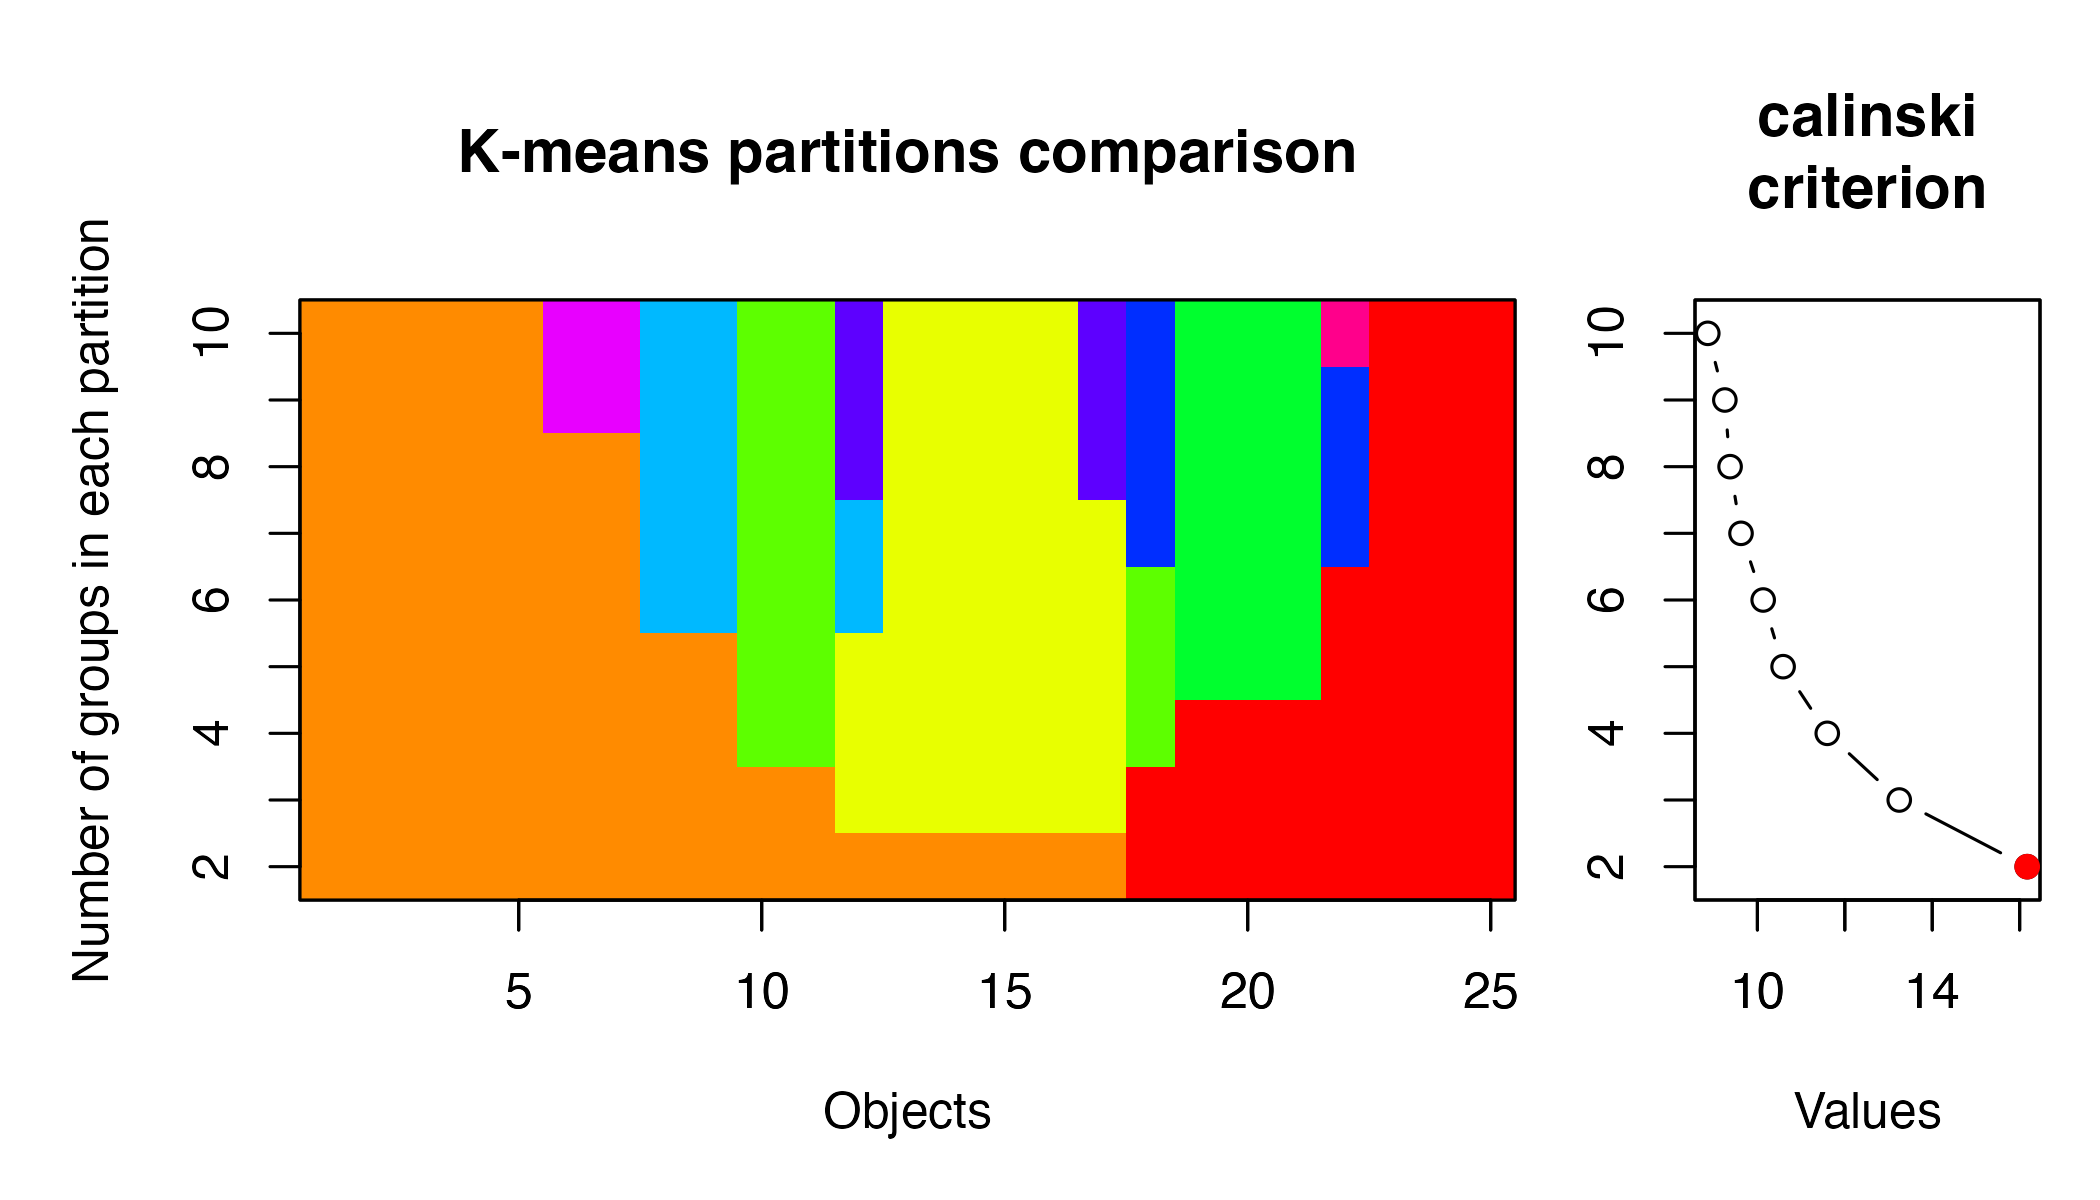
\includegraphics[keepaspectratio]{05_cluster_analysis_files/figure-beamer/unnamed-chunk-24-1.png}}
\end{frame}

\begin{frame}[fragile]{Визуализация k-means}
\protect\phantomsection\label{ux432ux438ux437ux443ux430ux43bux438ux437ux430ux446ux438ux44f-k-means}
Делается с помощью функции \texttt{fviz\_cluster} из пакета
\texttt{factoextra}.

\begin{columns}[T]
\begin{column}{0.5\linewidth}
\begin{Shaded}
\begin{Highlighting}[]
\FunctionTok{library}\NormalTok{(factoextra)}
\FunctionTok{fviz\_cluster}\NormalTok{(w\_kmeans, }\AttributeTok{data =}\NormalTok{ st\_w,}
             \AttributeTok{ggtheme =} \FunctionTok{theme\_bw}\NormalTok{())}
\end{Highlighting}
\end{Shaded}

\pandocbounded{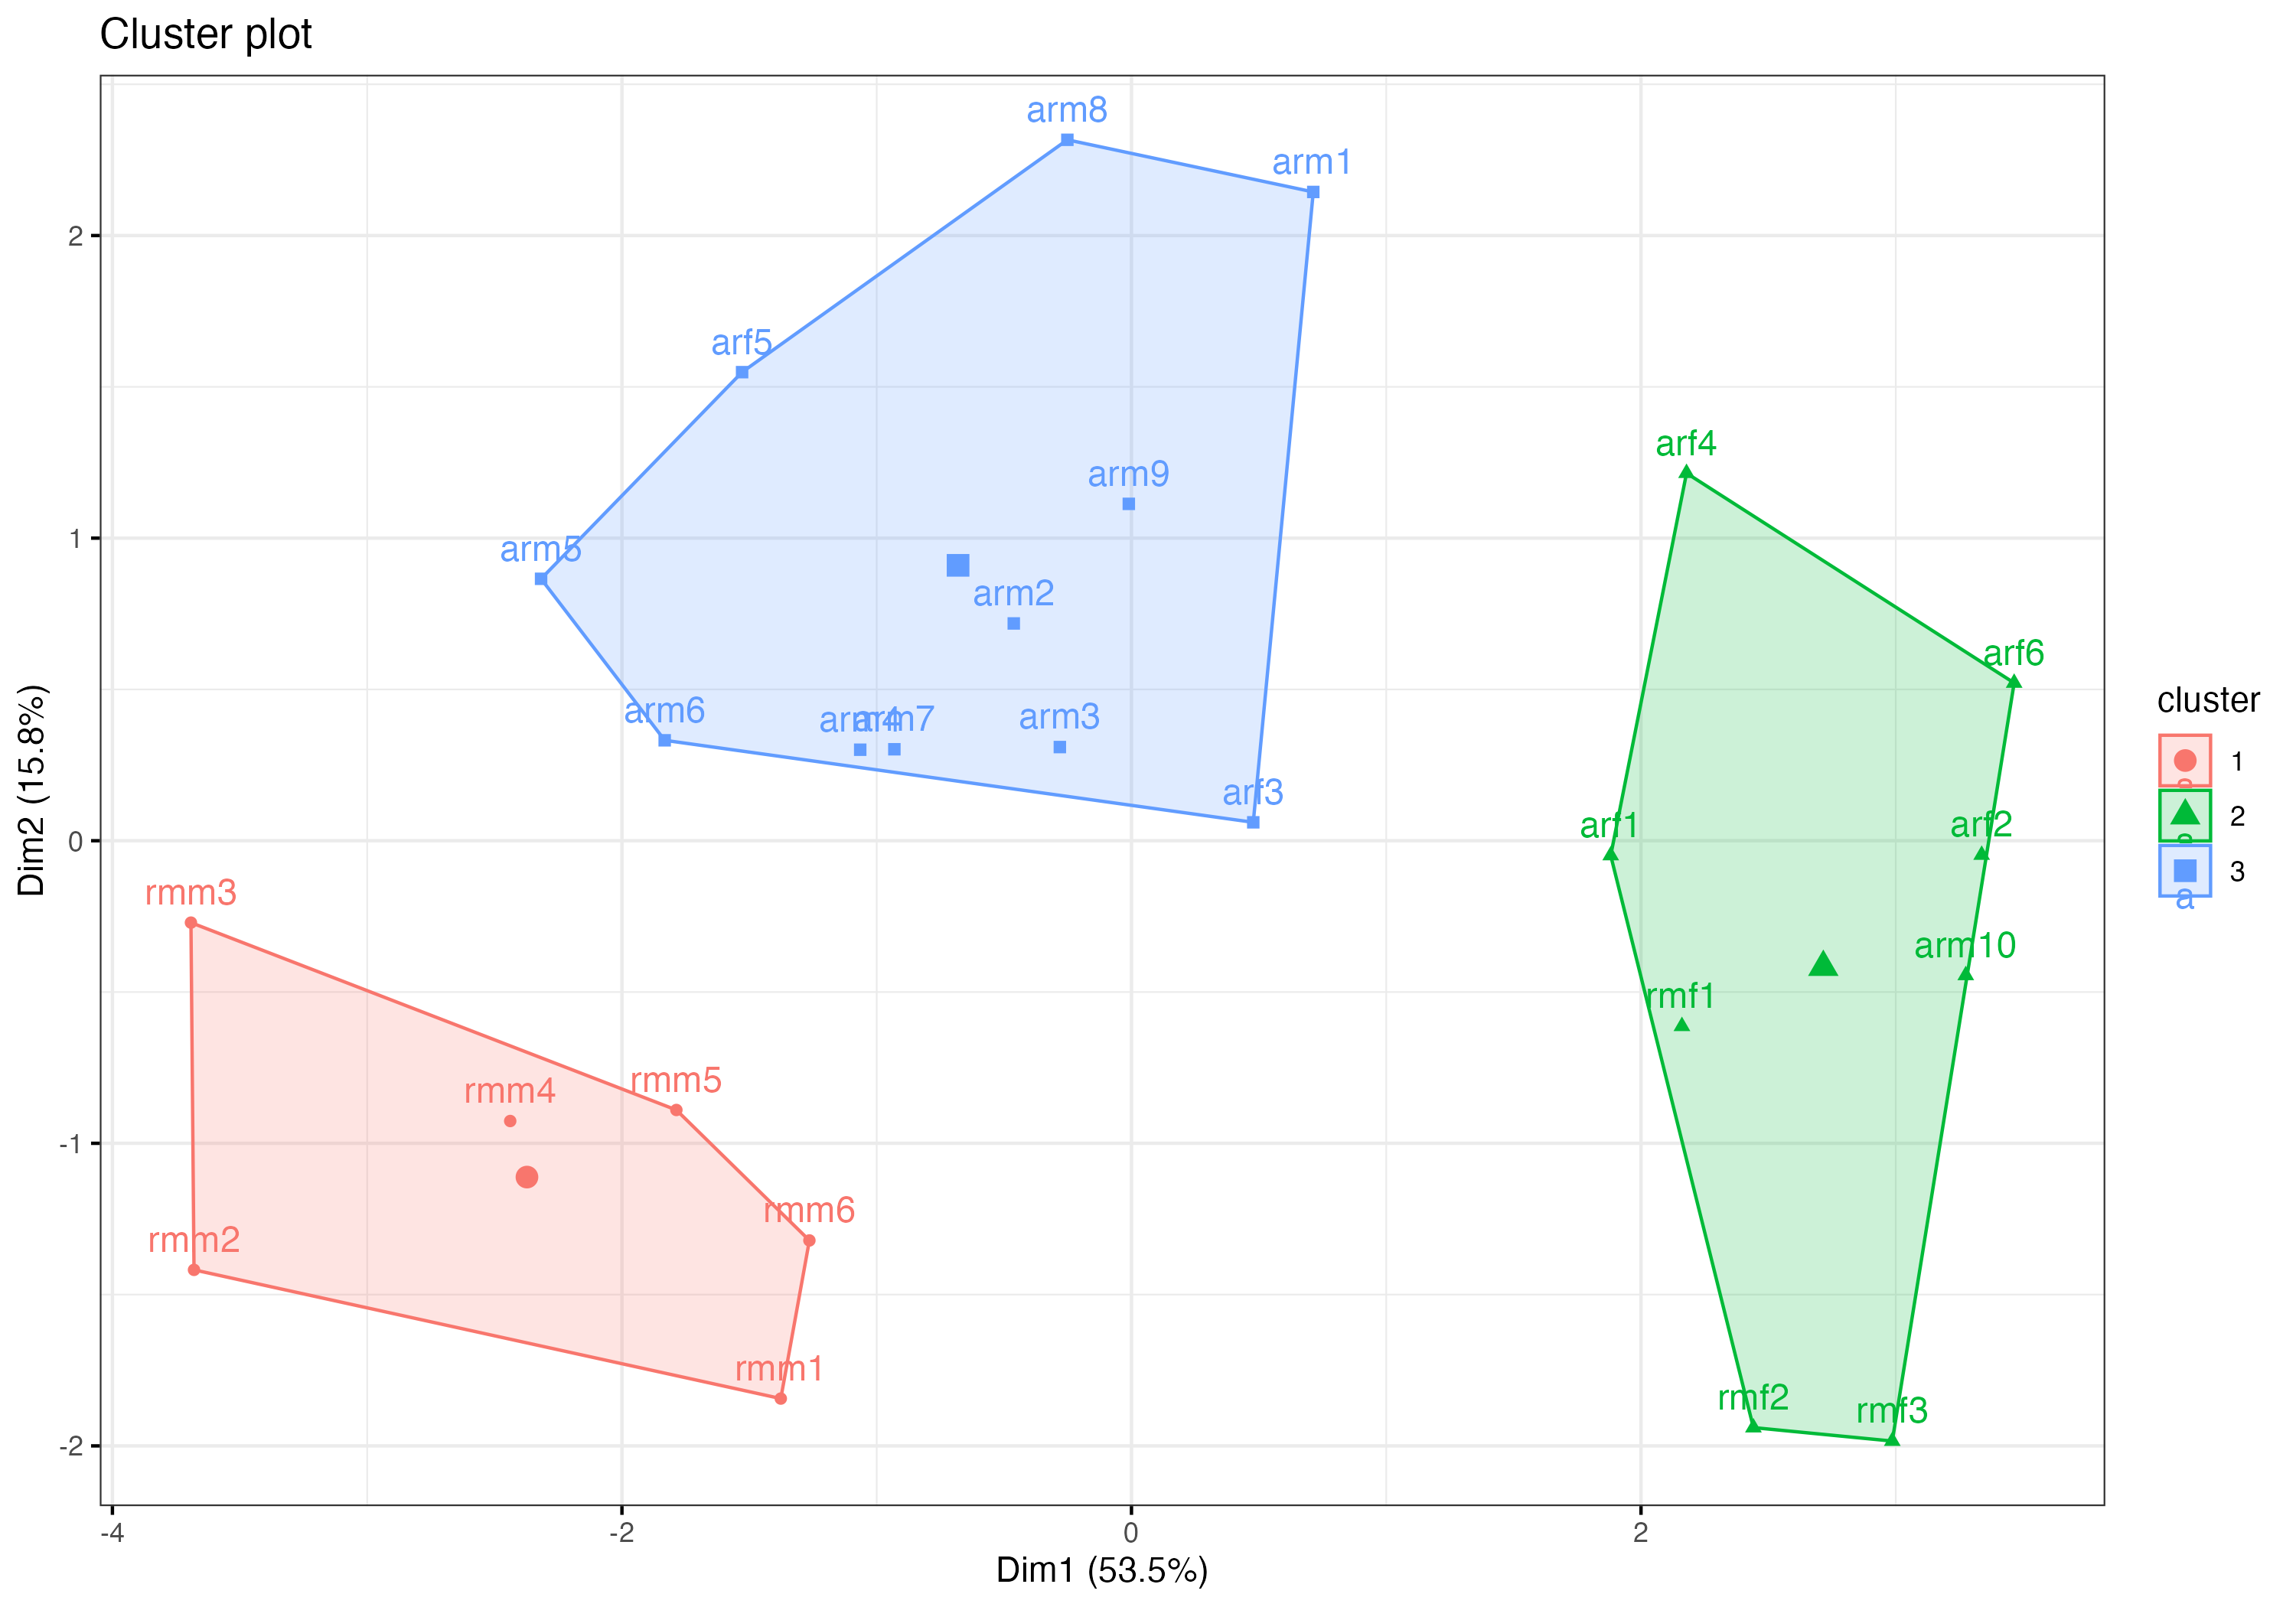
\includegraphics[keepaspectratio]{05_cluster_analysis_files/figure-beamer/unnamed-chunk-25-1.png}}
\end{column}

\begin{column}{0.5\linewidth}
\begin{Shaded}
\begin{Highlighting}[]
\NormalTok{w\_2k }\OtherTok{\textless{}{-}} \FunctionTok{kmeans}\NormalTok{(st\_w, }\AttributeTok{centers =} \DecValTok{2}\NormalTok{, }
               \AttributeTok{nstart =} \DecValTok{100}\NormalTok{)}

\FunctionTok{fviz\_cluster}\NormalTok{(w\_2k, }\AttributeTok{data =}\NormalTok{ st\_w,}
             \AttributeTok{ggtheme =} \FunctionTok{theme\_bw}\NormalTok{())}
\end{Highlighting}
\end{Shaded}

\pandocbounded{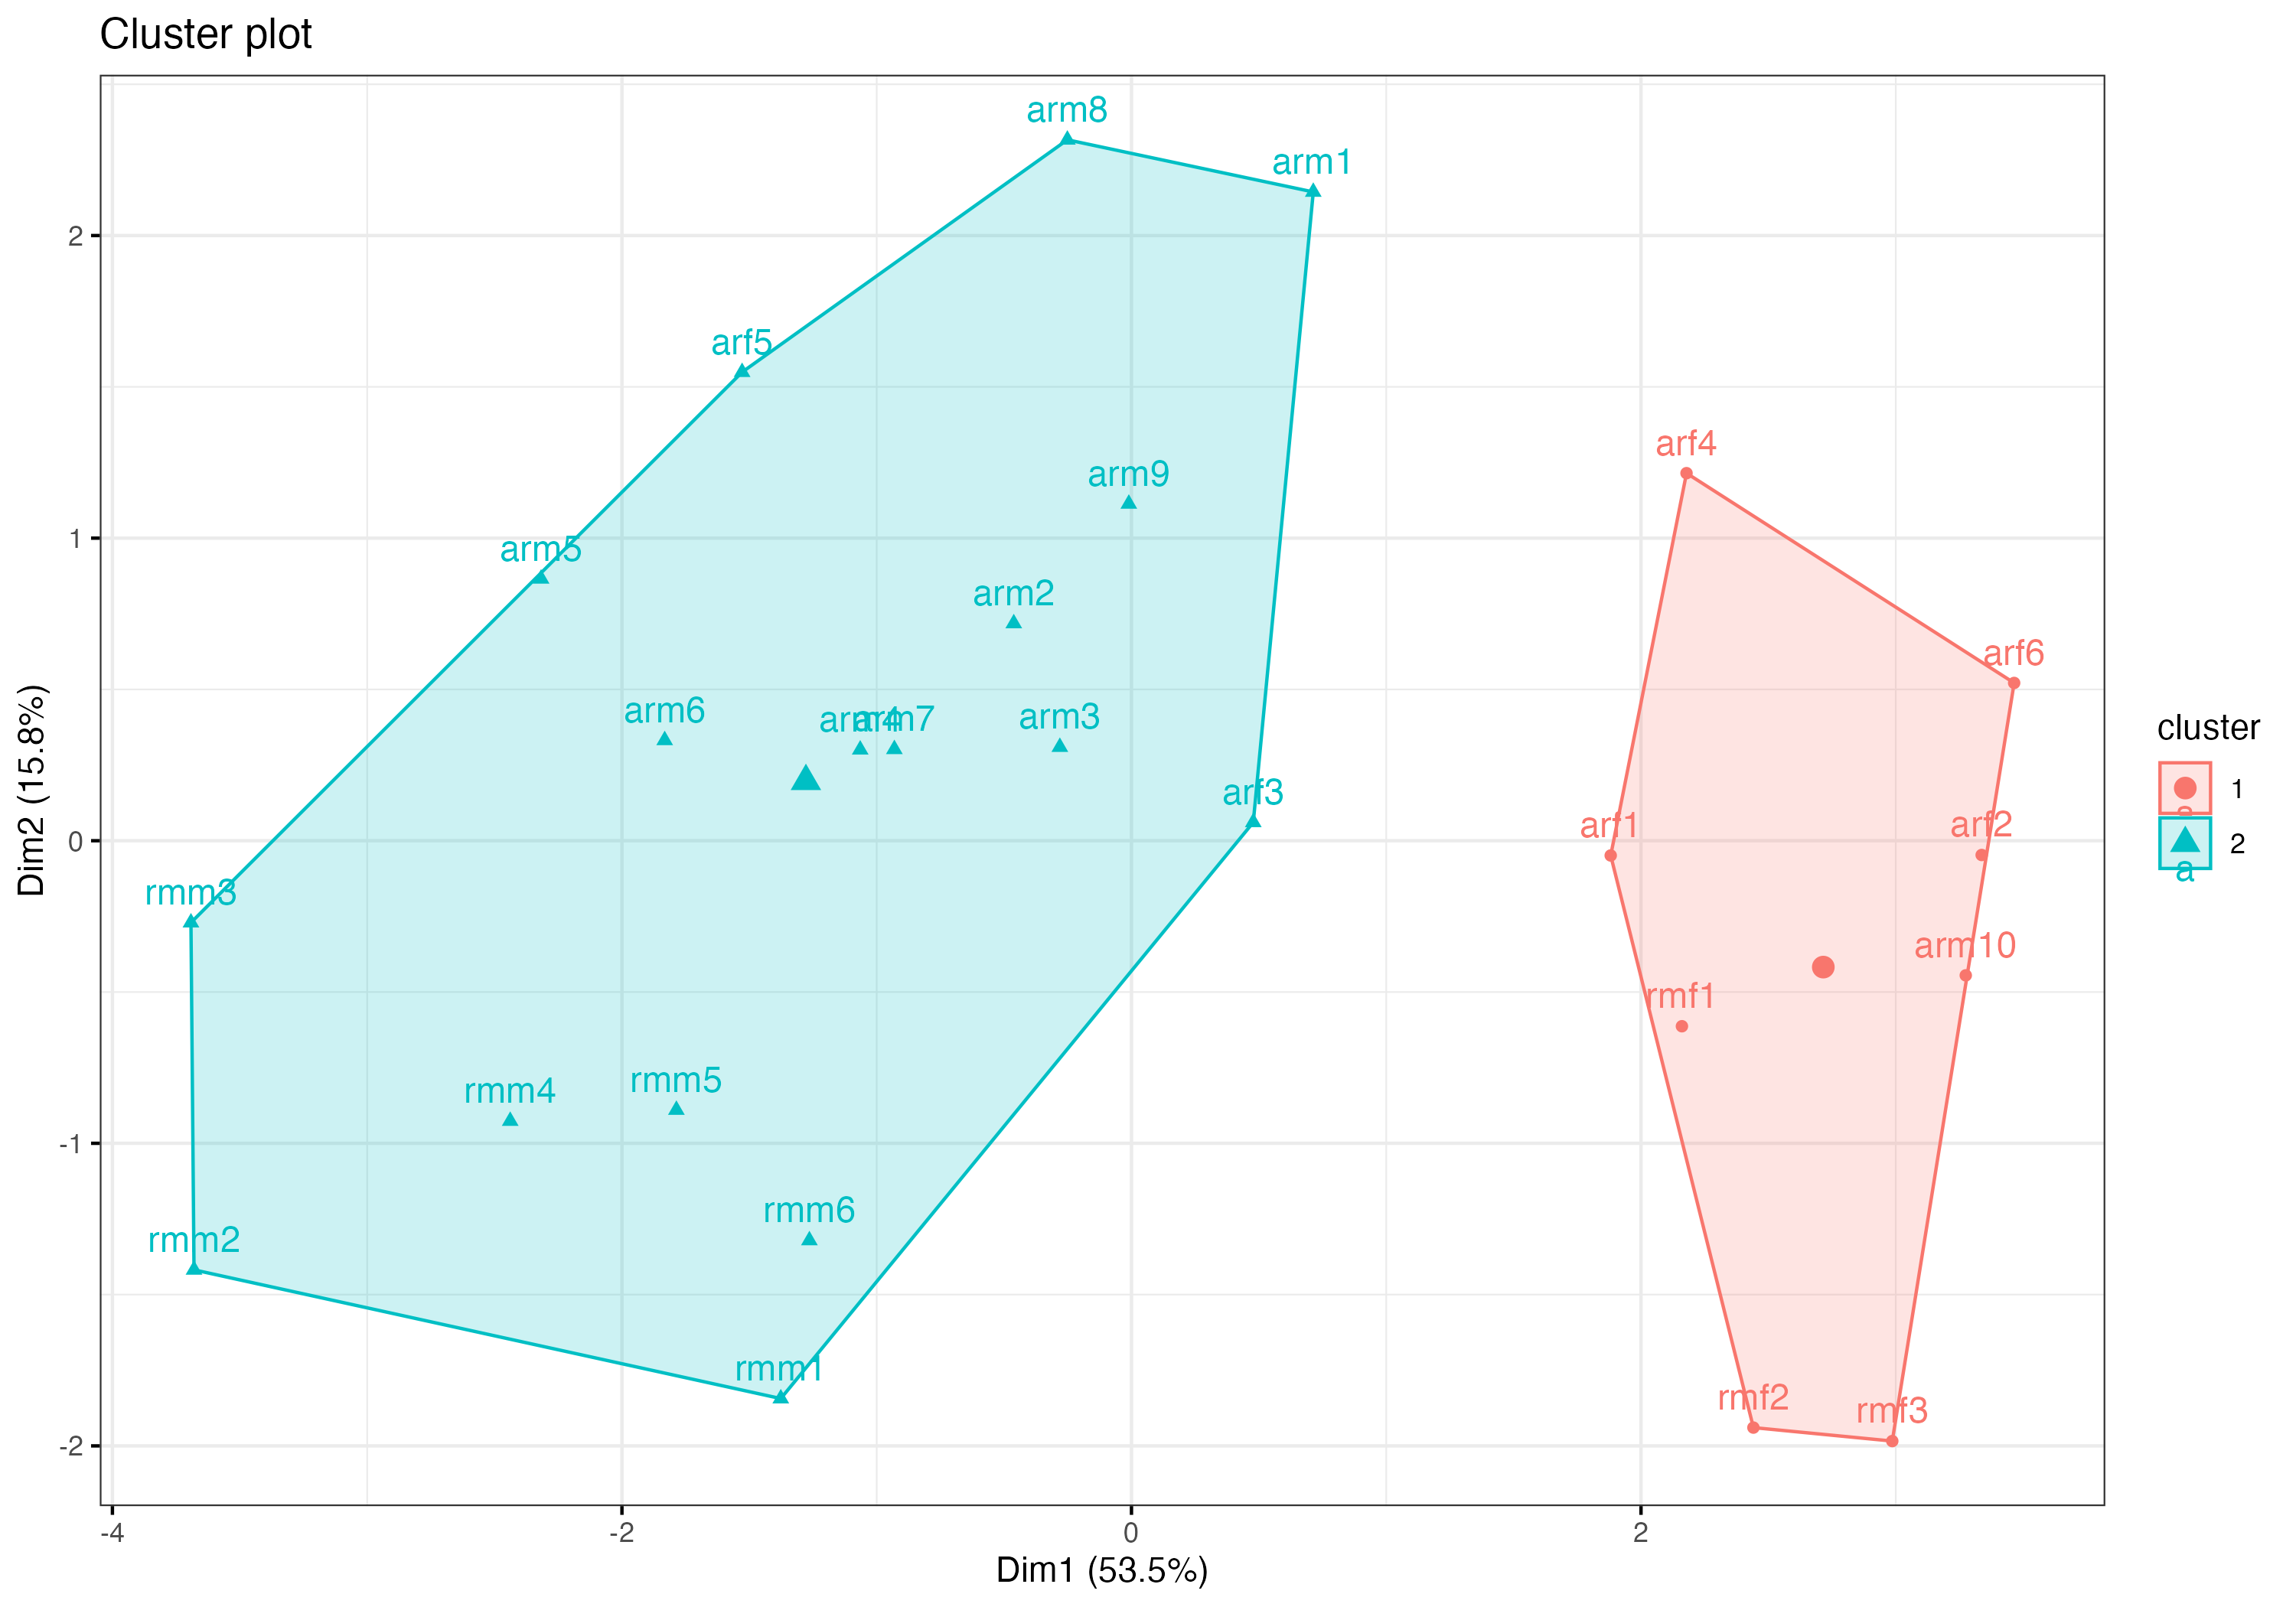
\includegraphics[keepaspectratio]{05_cluster_analysis_files/figure-beamer/unnamed-chunk-26-1.png}}
\end{column}
\end{columns}
\end{frame}

\begin{frame}[fragile]{Оценка качества кластеризации: ширина силуэта}
\protect\phantomsection\label{ux43eux446ux435ux43dux43aux430-ux43aux430ux447ux435ux441ux442ux432ux430-ux43aux43bux430ux441ux442ux435ux440ux438ux437ux430ux446ux438ux438-ux448ux438ux440ux438ux43dux430-ux441ux438ux43bux443ux44dux442ux430}
\begin{columns}[T]
\begin{column}{0.5\linewidth}
\begin{Shaded}
\begin{Highlighting}[]
\FunctionTok{plot}\NormalTok{(}\FunctionTok{silhouette}\NormalTok{(w\_kmeans}\SpecialCharTok{$}\NormalTok{cluster, d))}
\end{Highlighting}
\end{Shaded}

\pandocbounded{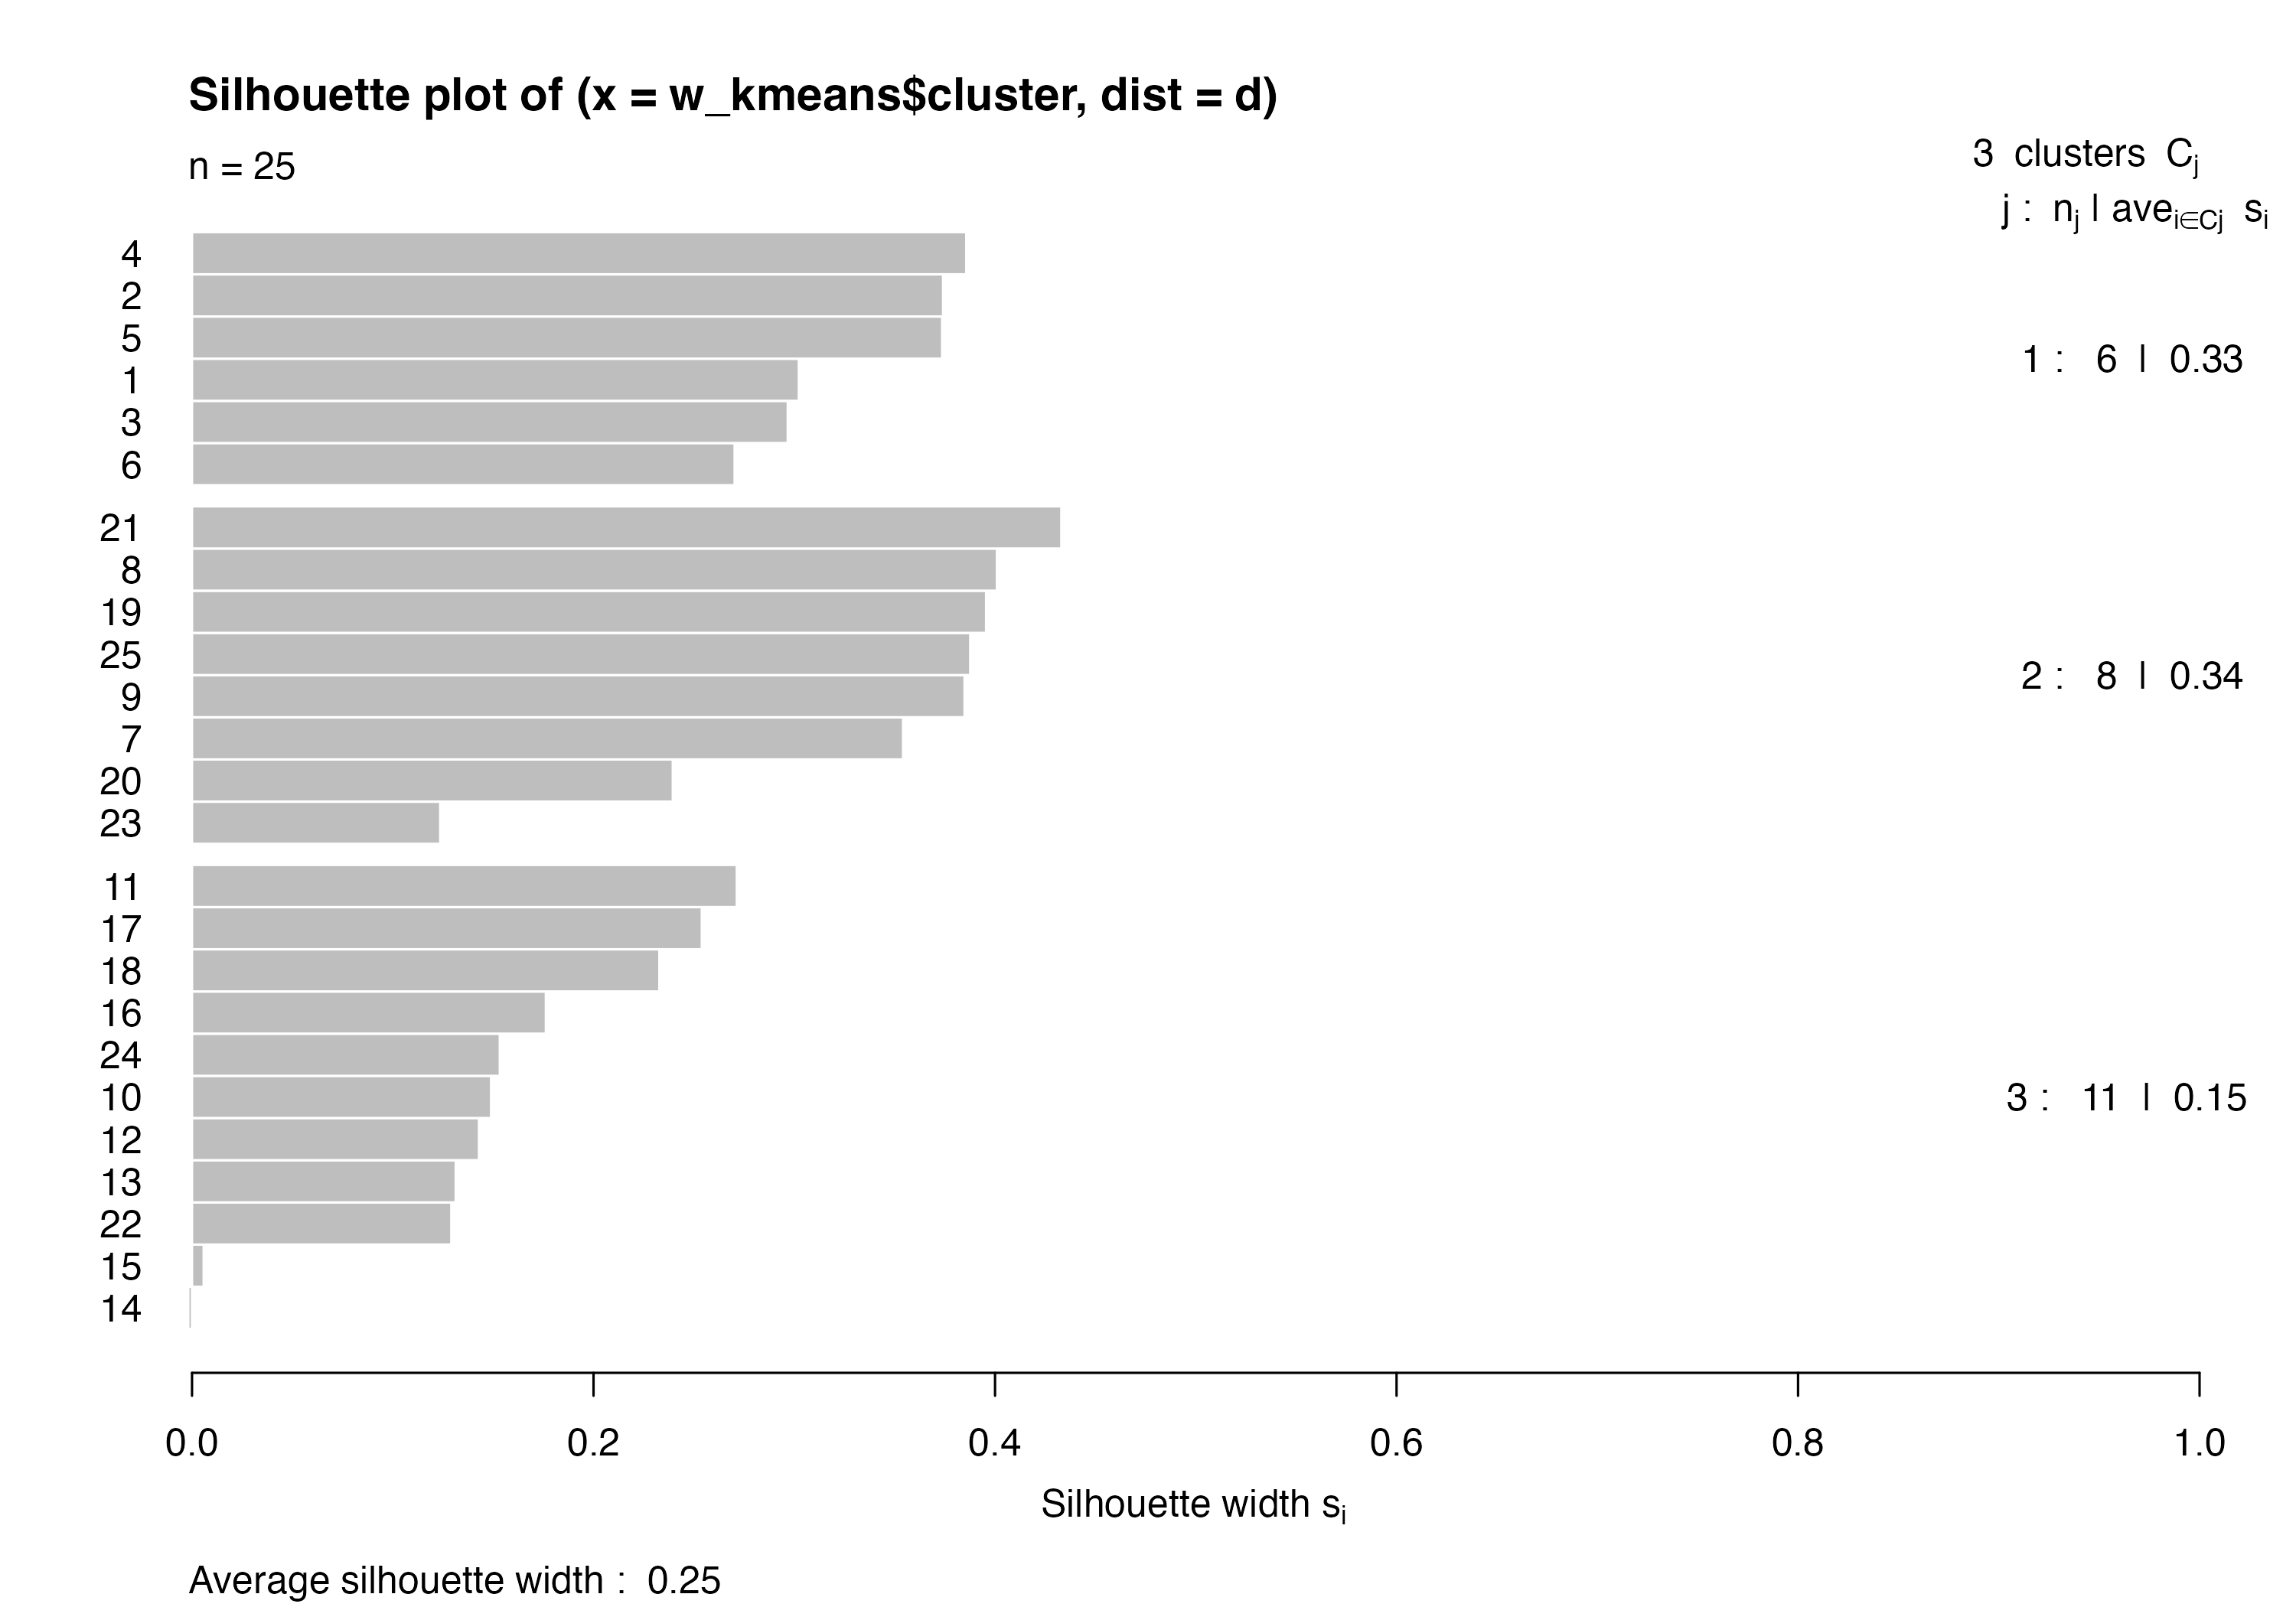
\includegraphics[keepaspectratio]{05_cluster_analysis_files/figure-beamer/unnamed-chunk-27-1.png}}
\end{column}

\begin{column}{0.5\linewidth}
\begin{Shaded}
\begin{Highlighting}[]
\FunctionTok{plot}\NormalTok{(}\FunctionTok{silhouette}\NormalTok{(w\_2k}\SpecialCharTok{$}\NormalTok{cluster, d))}
\end{Highlighting}
\end{Shaded}

\pandocbounded{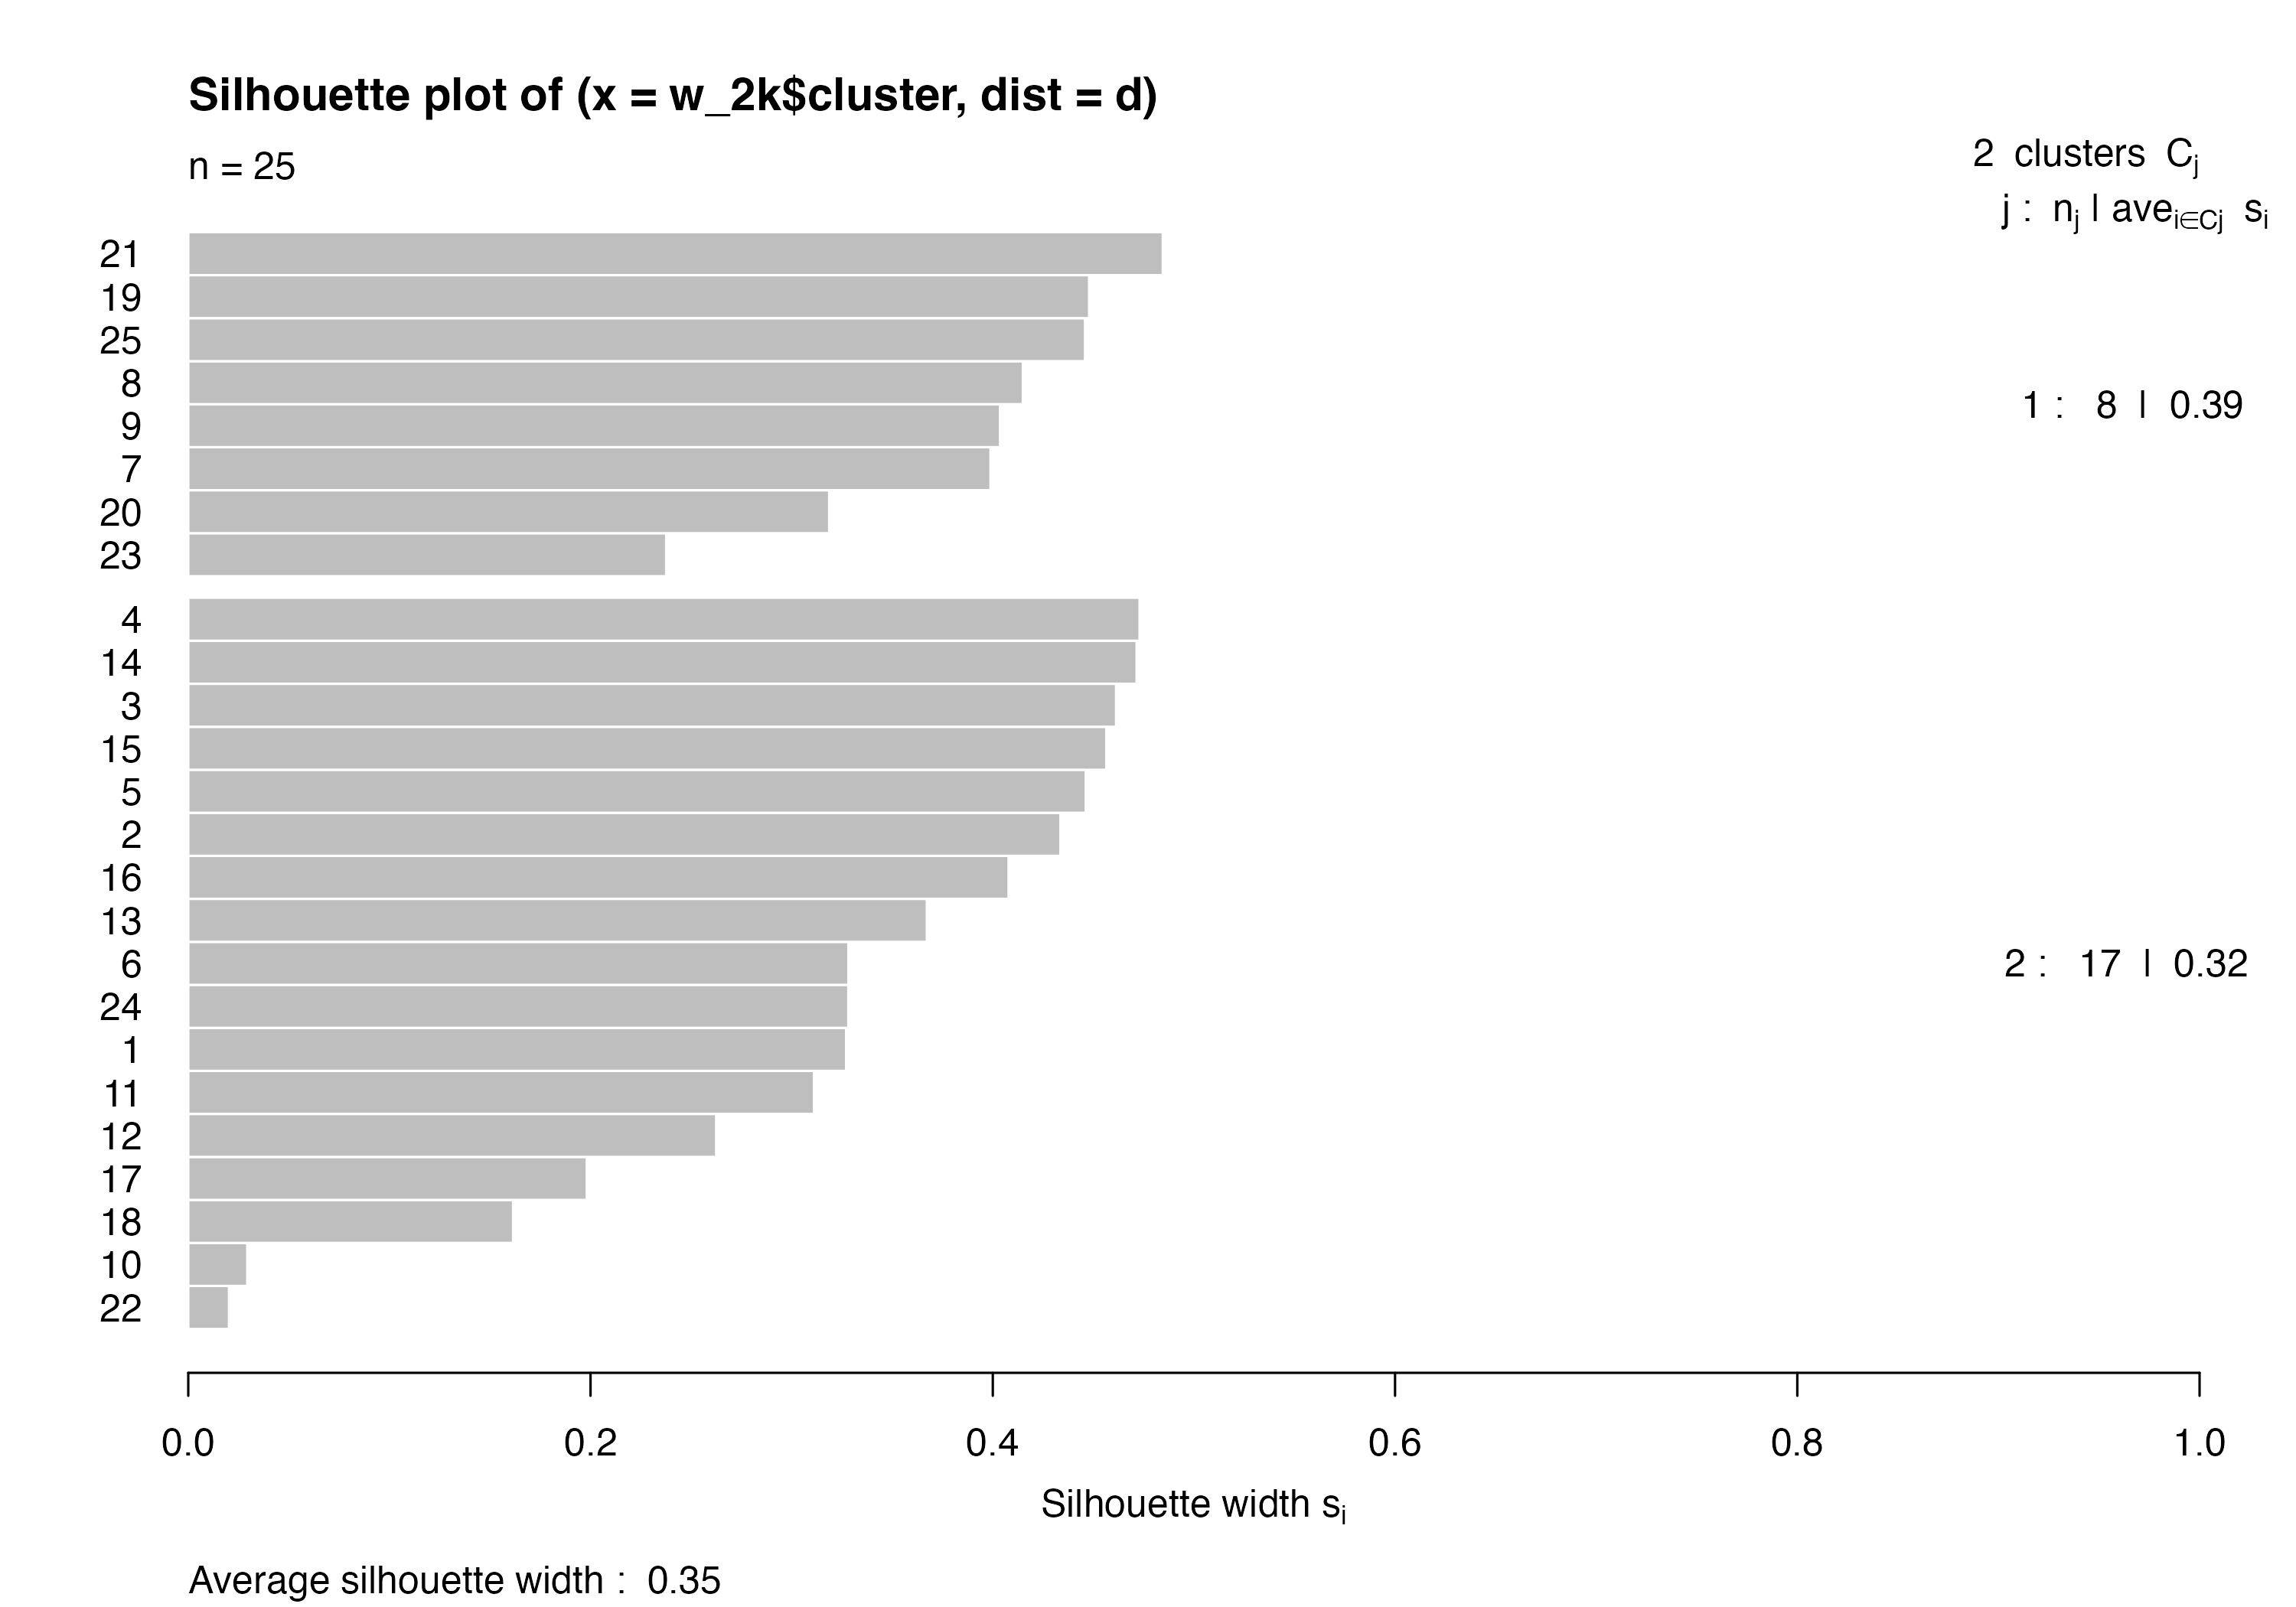
\includegraphics[keepaspectratio]{05_cluster_analysis_files/figure-beamer/unnamed-chunk-28-1.png}}
\end{column}
\end{columns}
\end{frame}

\begin{frame}[fragile]{Density-based spatial clustering of applications
with noise (DBSCAN)}
\protect\phantomsection\label{density-based-spatial-clustering-of-applications-with-noise-dbscan}
\begin{columns}[T]
\begin{column}{0.5\linewidth}
Основанная на плотности пространственная кластеризация для приложений с
шумами --- метод, более подходящий для ``вложенных'' кластеров. Основан
на распределении плотности точек.

\pandocbounded{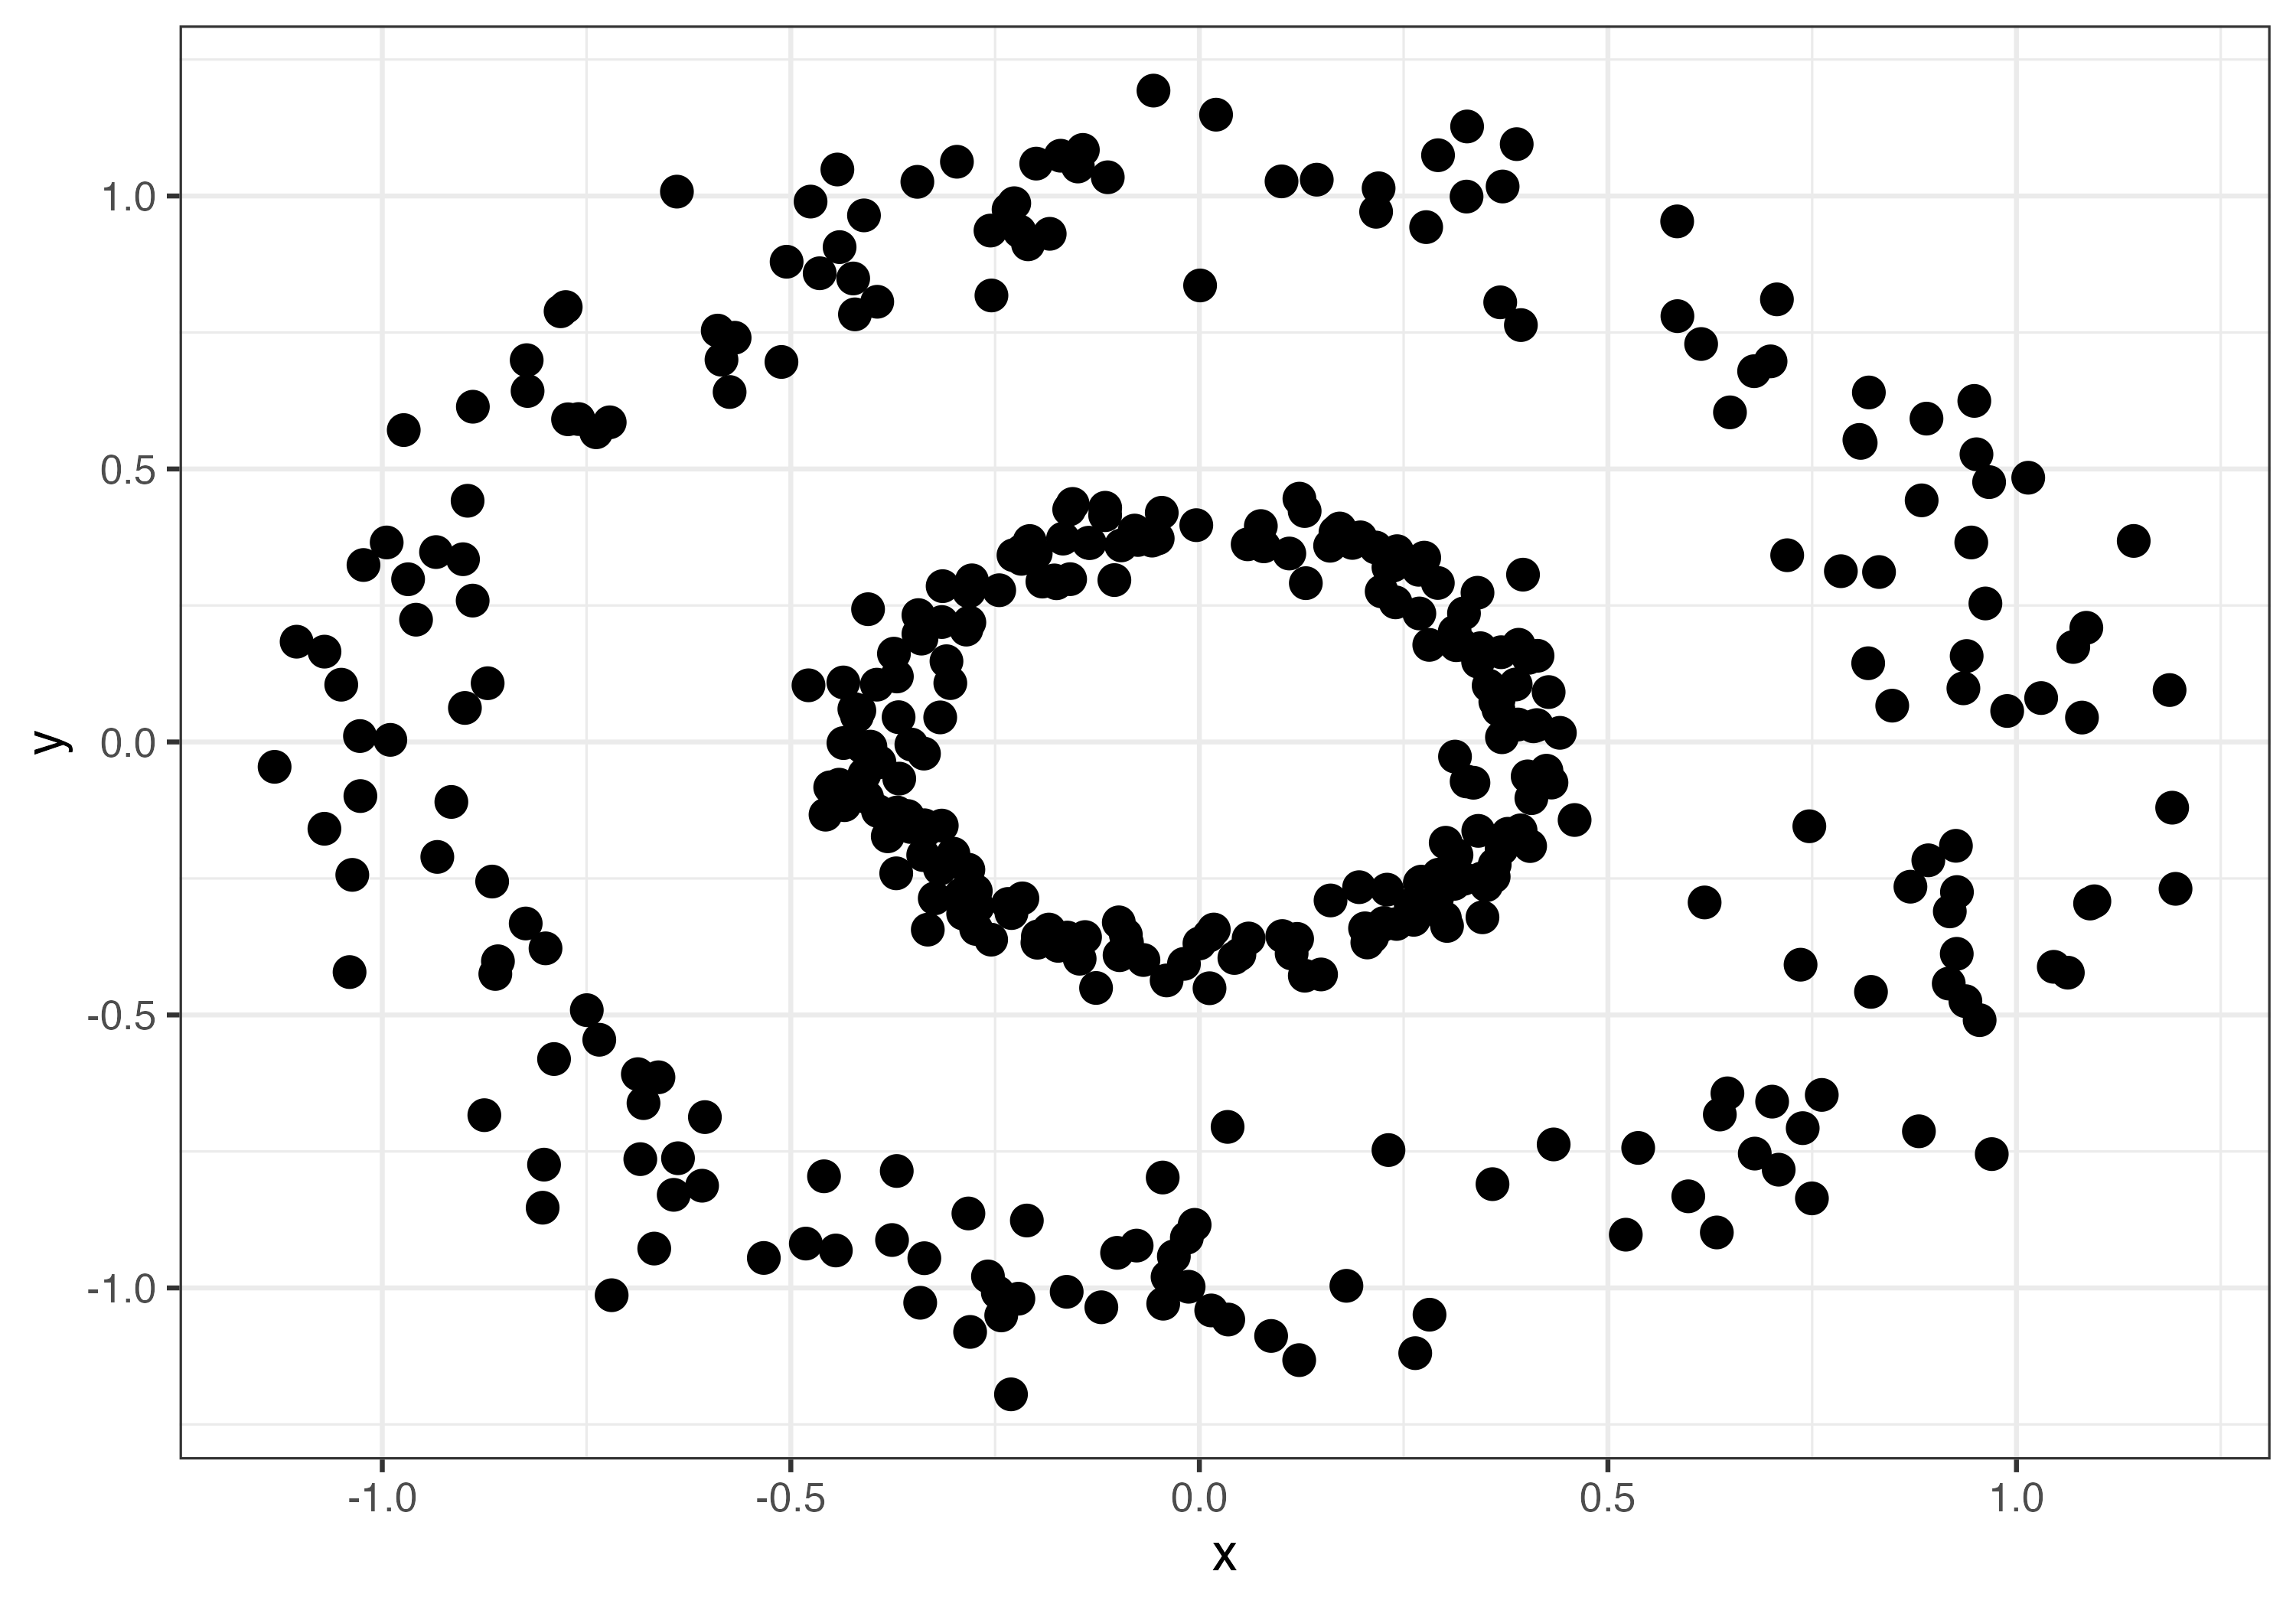
\includegraphics[keepaspectratio]{05_cluster_analysis_files/figure-beamer/unnamed-chunk-29-1.png}}
\end{column}

\begin{column}{0.5\linewidth}
Работает с данными, с которыми другие методы кластеризации не могут
справиться (K-means в примере).

\begin{Shaded}
\begin{Highlighting}[]
\FunctionTok{set.seed}\NormalTok{(}\DecValTok{123}\NormalTok{)}
\NormalTok{circle\_kmeans }\OtherTok{\textless{}{-}} \FunctionTok{kmeans}\NormalTok{(multi, }\AttributeTok{centers =} \DecValTok{2}\NormalTok{, }\AttributeTok{nstart =} \DecValTok{20}\NormalTok{)}
\NormalTok{my\_col\_circle }\OtherTok{\textless{}{-}} \FunctionTok{c}\NormalTok{(}\StringTok{"\#2E9FDF"}\NormalTok{, }\StringTok{"\#E7B800"}\NormalTok{)}
\FunctionTok{fviz\_cluster}\NormalTok{(circle\_kmeans, }
             \AttributeTok{data =}\NormalTok{ multi, }\AttributeTok{palette =}\NormalTok{ my\_col\_circle)}
\end{Highlighting}
\end{Shaded}

\pandocbounded{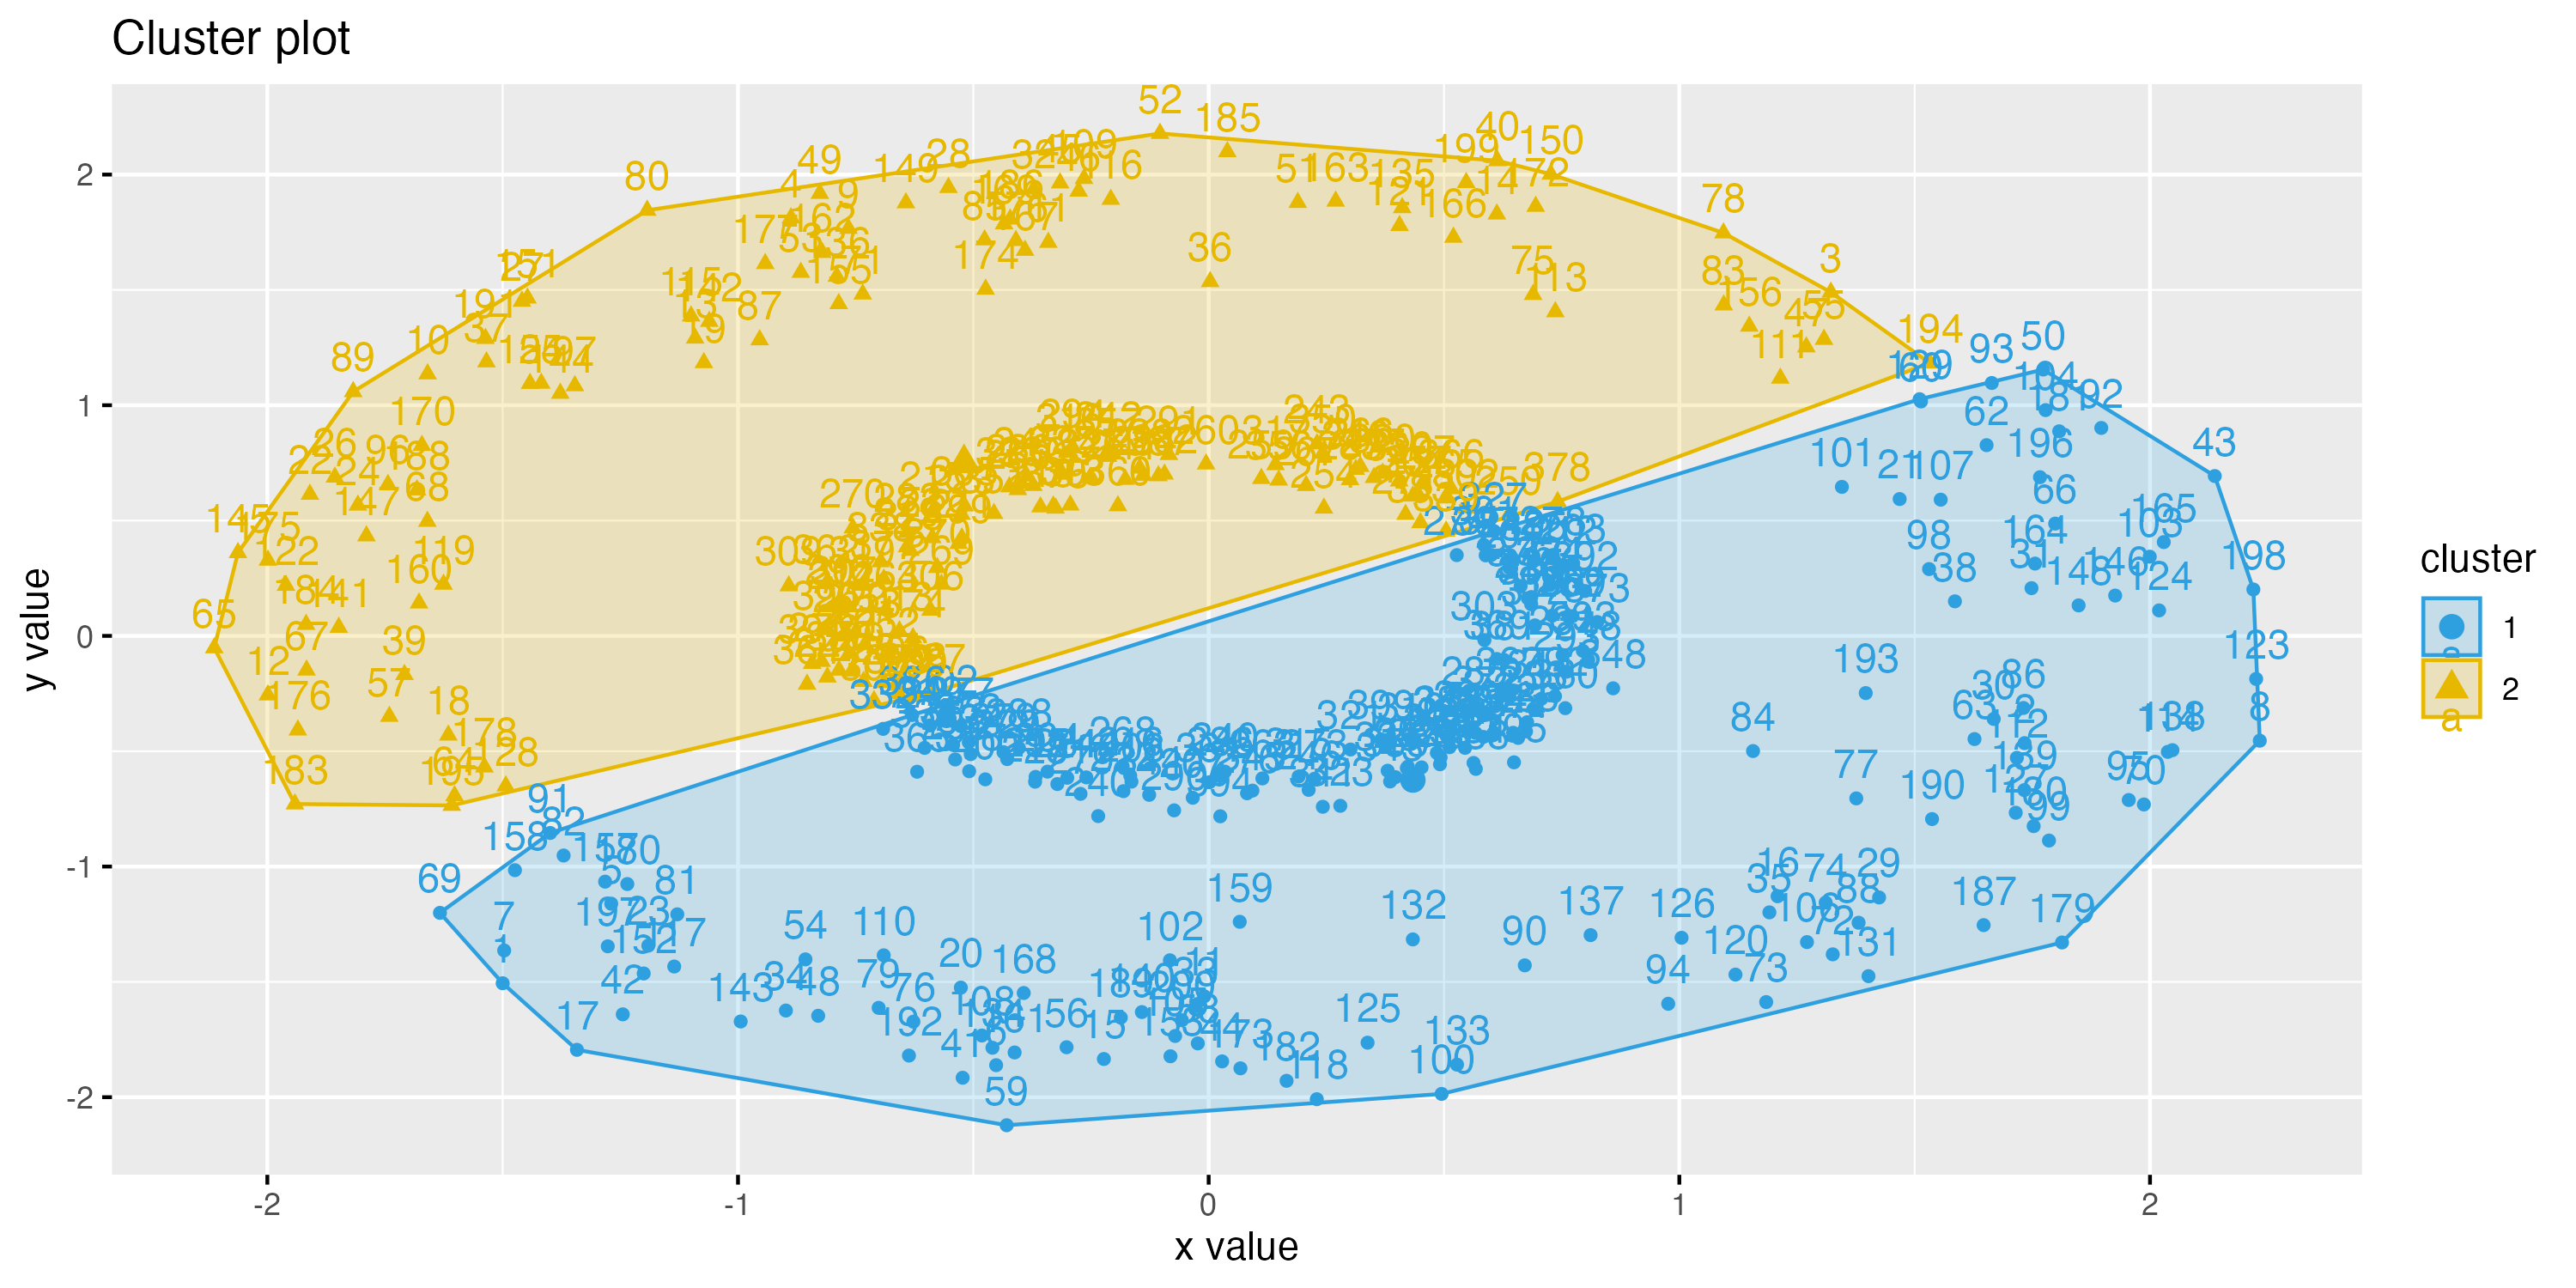
\includegraphics[keepaspectratio]{05_cluster_analysis_files/figure-beamer/unnamed-chunk-30-1.png}}
\end{column}
\end{columns}
\end{frame}

\begin{frame}[fragile]{Принцип работы DBSCAN}
\protect\phantomsection\label{ux43fux440ux438ux43dux446ux438ux43f-ux440ux430ux431ux43eux442ux44b-dbscan}
Кластеры выбираются на основе плотности расположения точек. В результате
в единый кластер объединяются близко расположенные друг к другу точки.

Задаваемые параметры:

\begin{itemize}
\tightlist
\item
  радиус расстояния, на котором должны рассматриваться близлежащие точки
  (\texttt{eps})
\item
  минимальное количество точек, которые расположены в круге этого
  радиуса (\texttt{minPts})
\end{itemize}

Сore points --- точки, от которых можем присоединять в кластер новые
точки и рядом с которыми расположено \texttt{minPts} количество точек.

Пограничные точки --- те, на которых кластер заканчивается.

Остальные точки считаются шумом и выбросами.
\end{frame}

\begin{frame}[fragile]{DBSCAN в R}
\protect\phantomsection\label{dbscan-ux432-r}
Провести такую кластеризацию можно с помощью функции \texttt{dbscan} из
пакета \texttt{dbscan}.

\pandocbounded{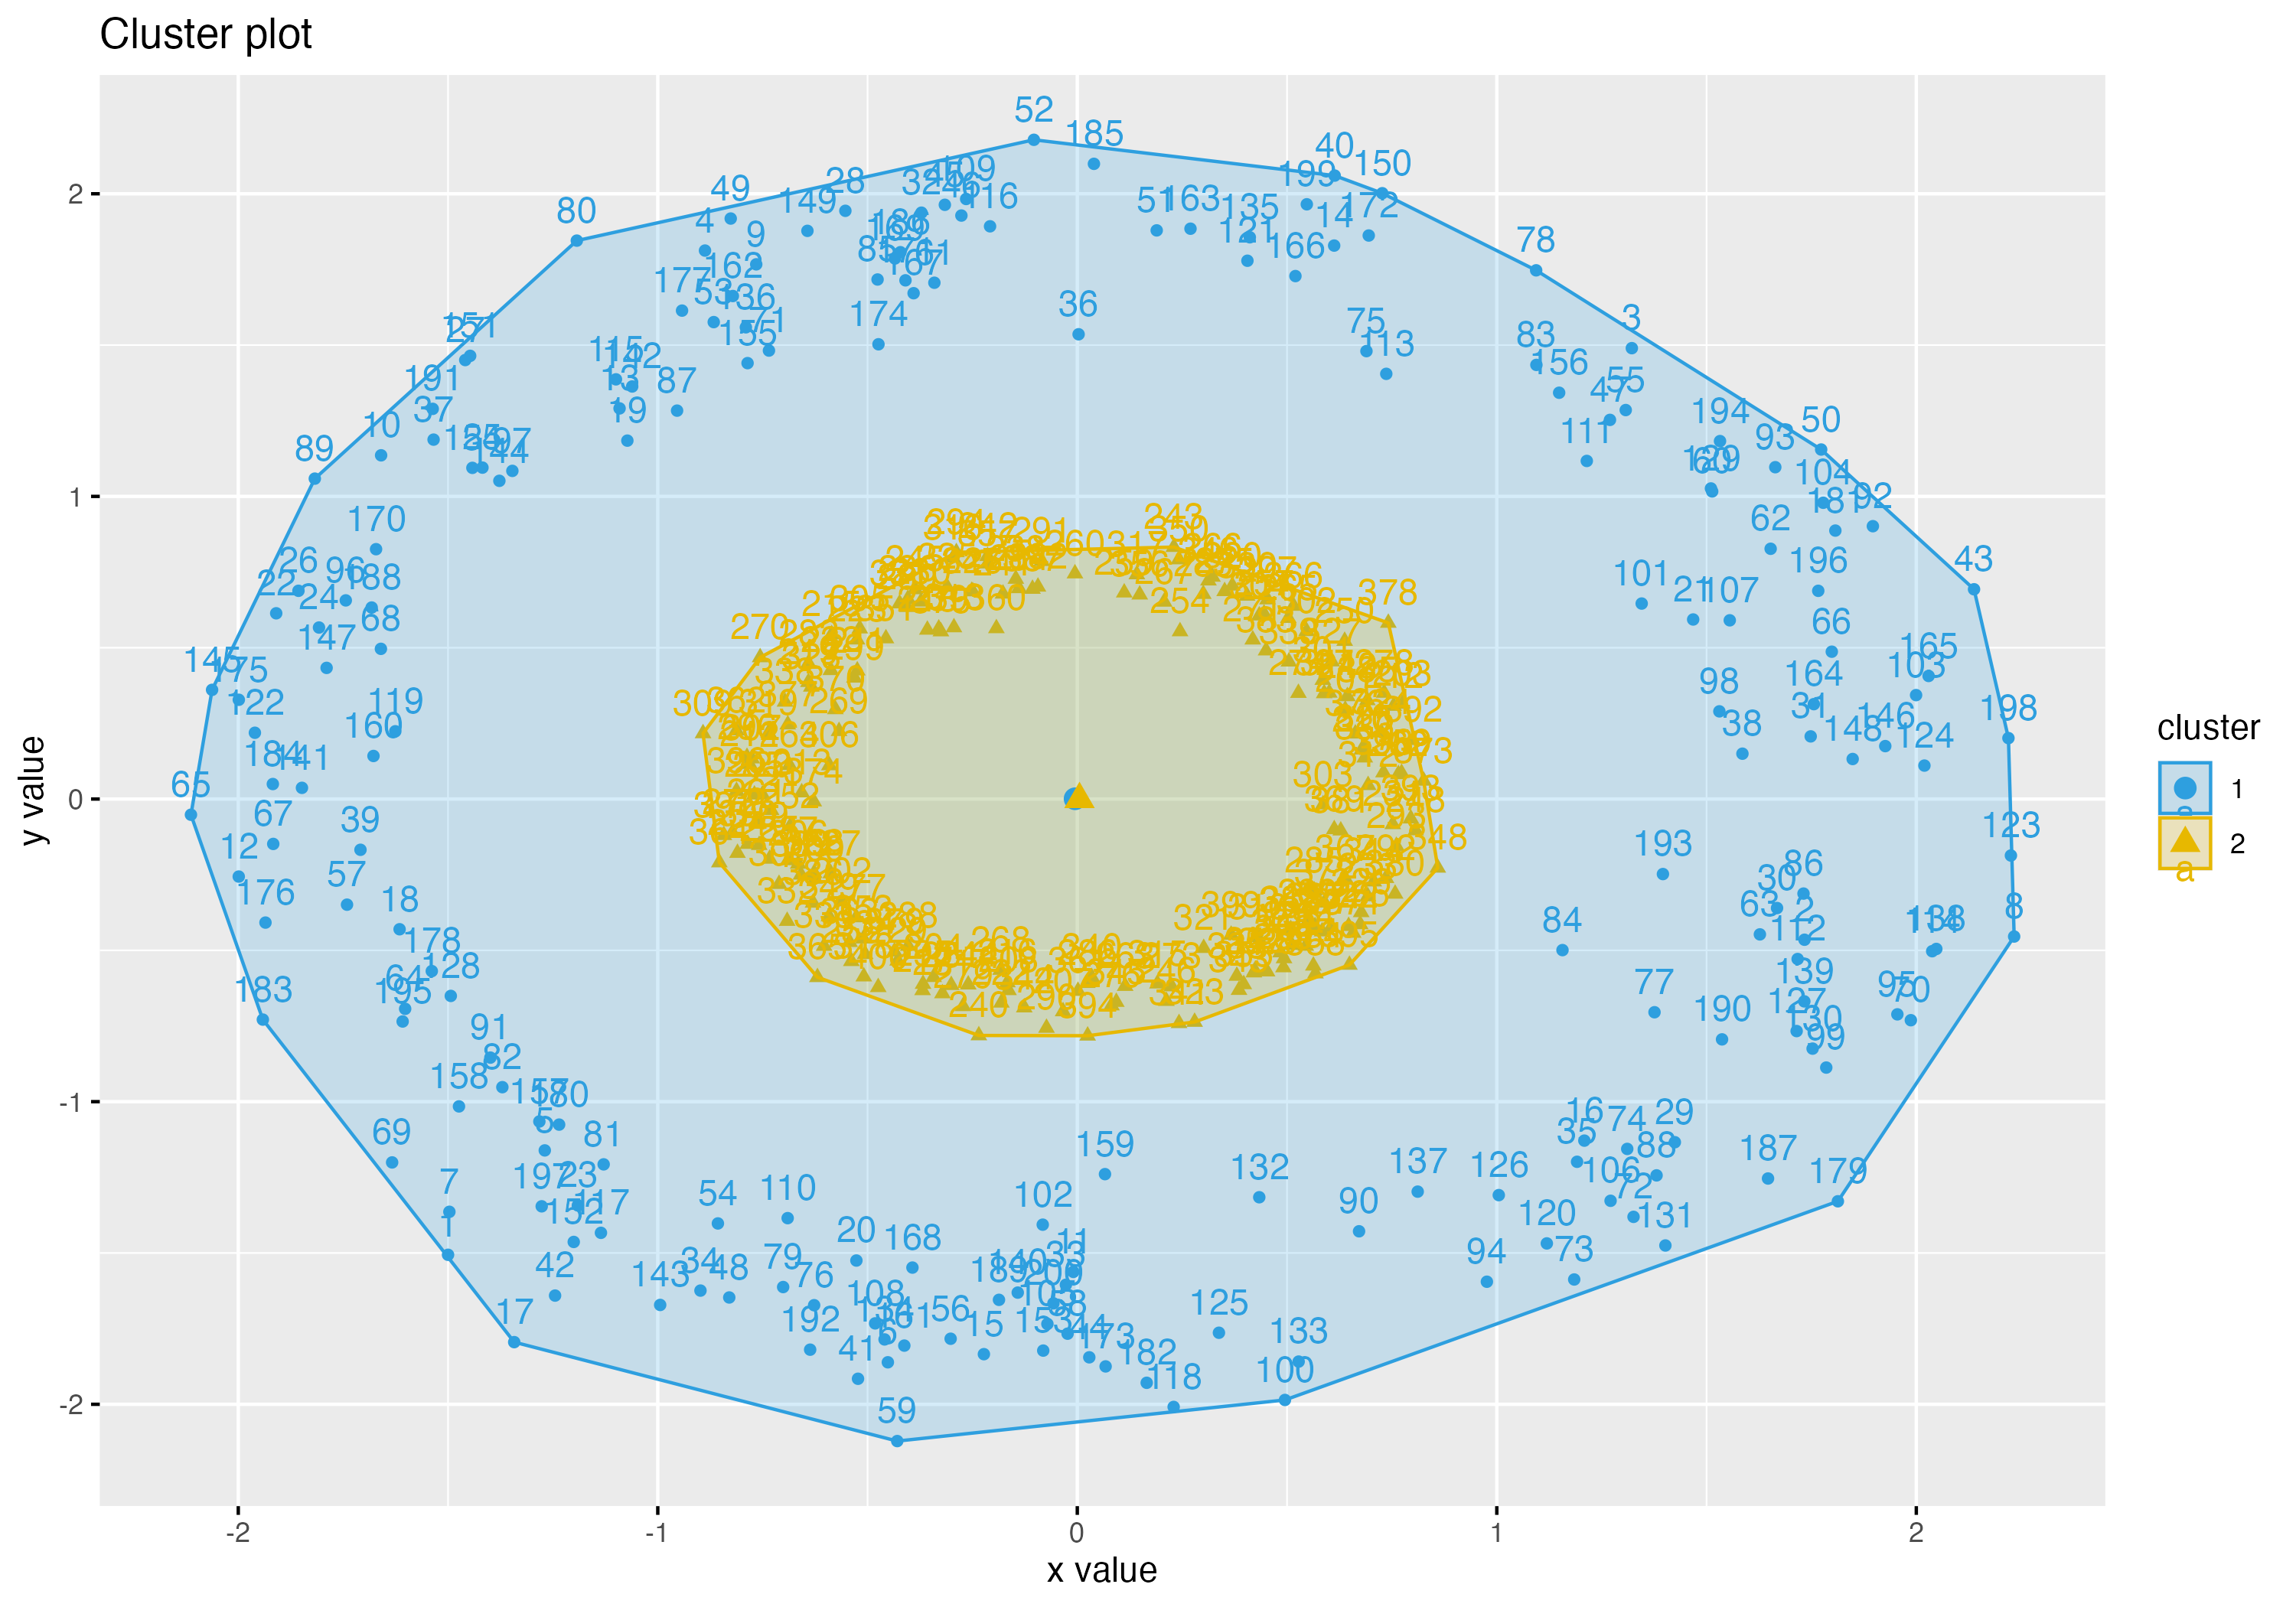
\includegraphics[keepaspectratio]{05_cluster_analysis_files/figure-beamer/unnamed-chunk-31-1.png}}
\end{frame}

\begin{frame}[fragile]{Epsilon --- выбираем расстояние для радиуса}
\protect\phantomsection\label{epsilon-ux432ux44bux431ux438ux440ux430ux435ux43c-ux440ux430ux441ux441ux442ux43eux44fux43dux438ux435-ux434ux43bux44f-ux440ux430ux434ux438ux443ux441ux430}
\textbf{График k-расстояний (k-distance plot)}

\begin{enumerate}
\item
  Вычисляется среднее значение расстояний каждой точки до ее k ближайших
  соседей.
\item
  k-расстояния отображаются в порядке возрастания.
\end{enumerate}

Если на графике есть ``колено'' --- значительный перегиб, будет легко
найти нужное значение радиуса.

\begin{columns}[T]
\begin{column}{0.5\linewidth}
\begin{Shaded}
\begin{Highlighting}[]
\FunctionTok{kNNdistplot}\NormalTok{(multi, }\AttributeTok{k =} \DecValTok{5}\NormalTok{)}
\FunctionTok{abline}\NormalTok{(}\AttributeTok{h =} \FloatTok{0.23}\NormalTok{, }\AttributeTok{lty =} \DecValTok{2}\NormalTok{)}
\end{Highlighting}
\end{Shaded}

\pandocbounded{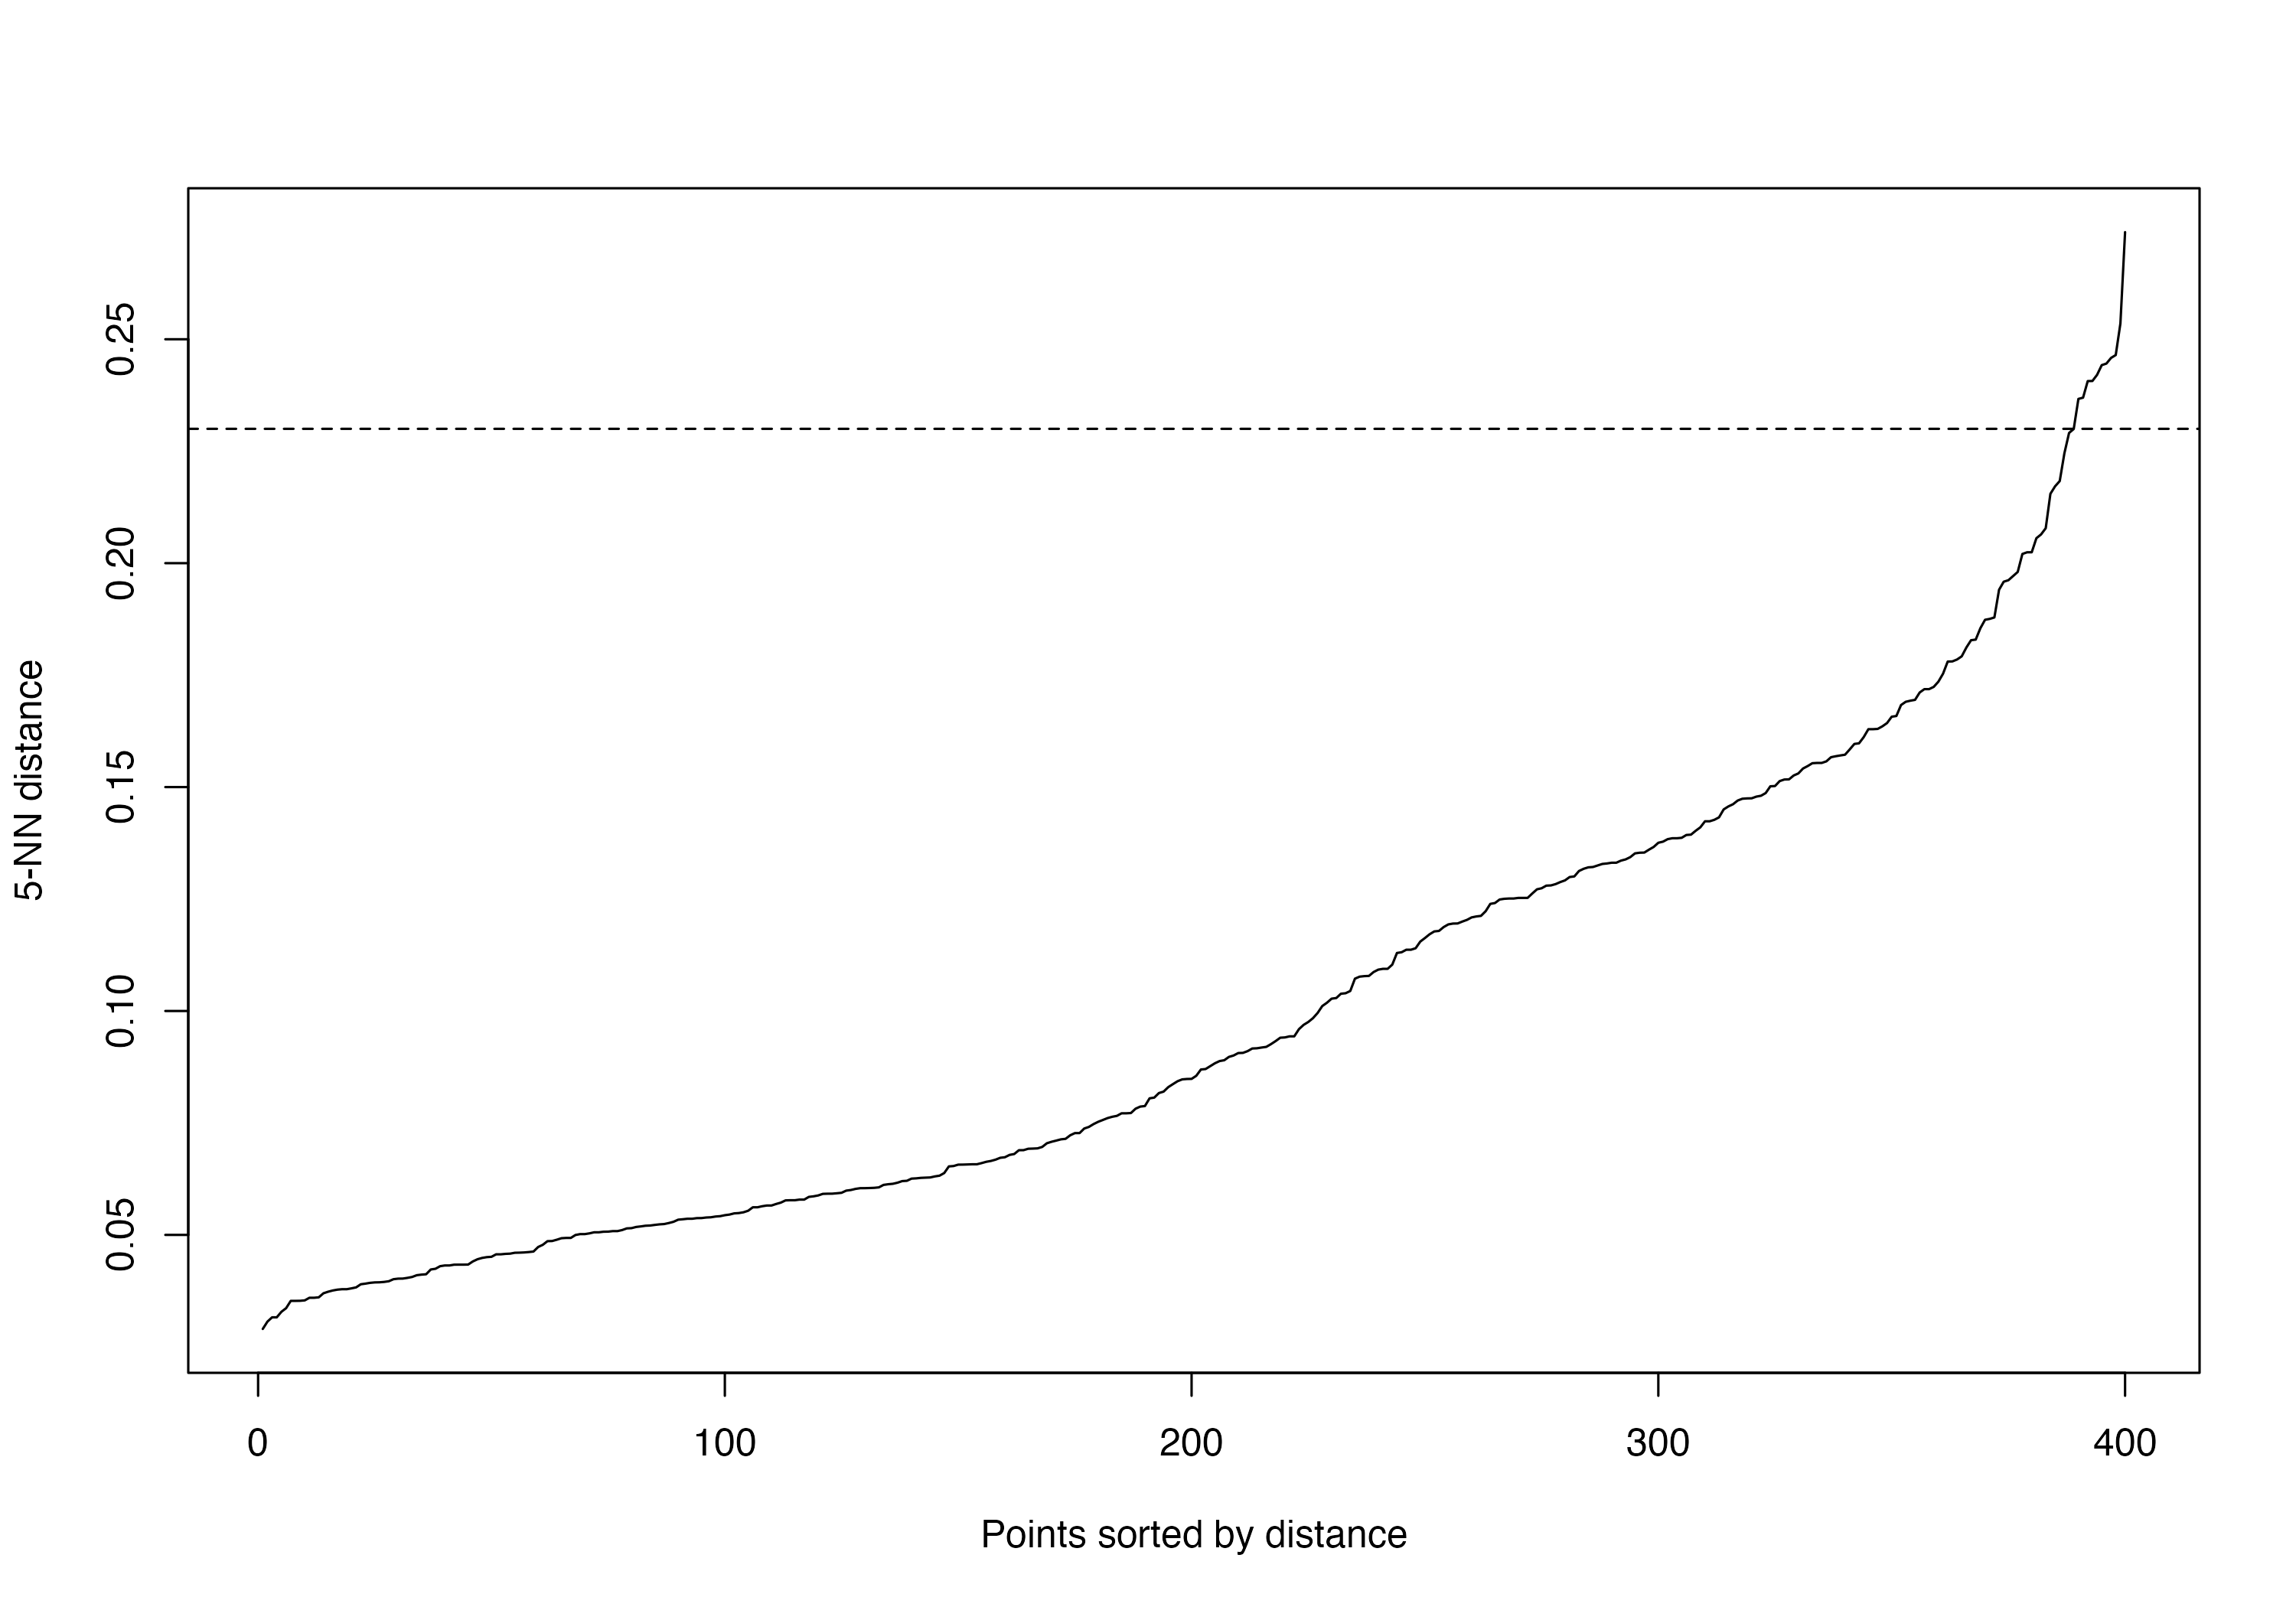
\includegraphics[keepaspectratio]{05_cluster_analysis_files/figure-beamer/unnamed-chunk-32-1.png}}
\end{column}

\begin{column}{0.5\linewidth}
\begin{Shaded}
\begin{Highlighting}[]
\NormalTok{circle\_dbscan }\OtherTok{\textless{}{-}} \FunctionTok{dbscan}\NormalTok{(multi, }\FloatTok{0.23}\NormalTok{, }\DecValTok{5}\NormalTok{)}
\FunctionTok{fviz\_cluster}\NormalTok{(circle\_dbscan, }\AttributeTok{data =}\NormalTok{ multi,}
             \AttributeTok{palette =}\NormalTok{ my\_col\_circle)}
\end{Highlighting}
\end{Shaded}

\pandocbounded{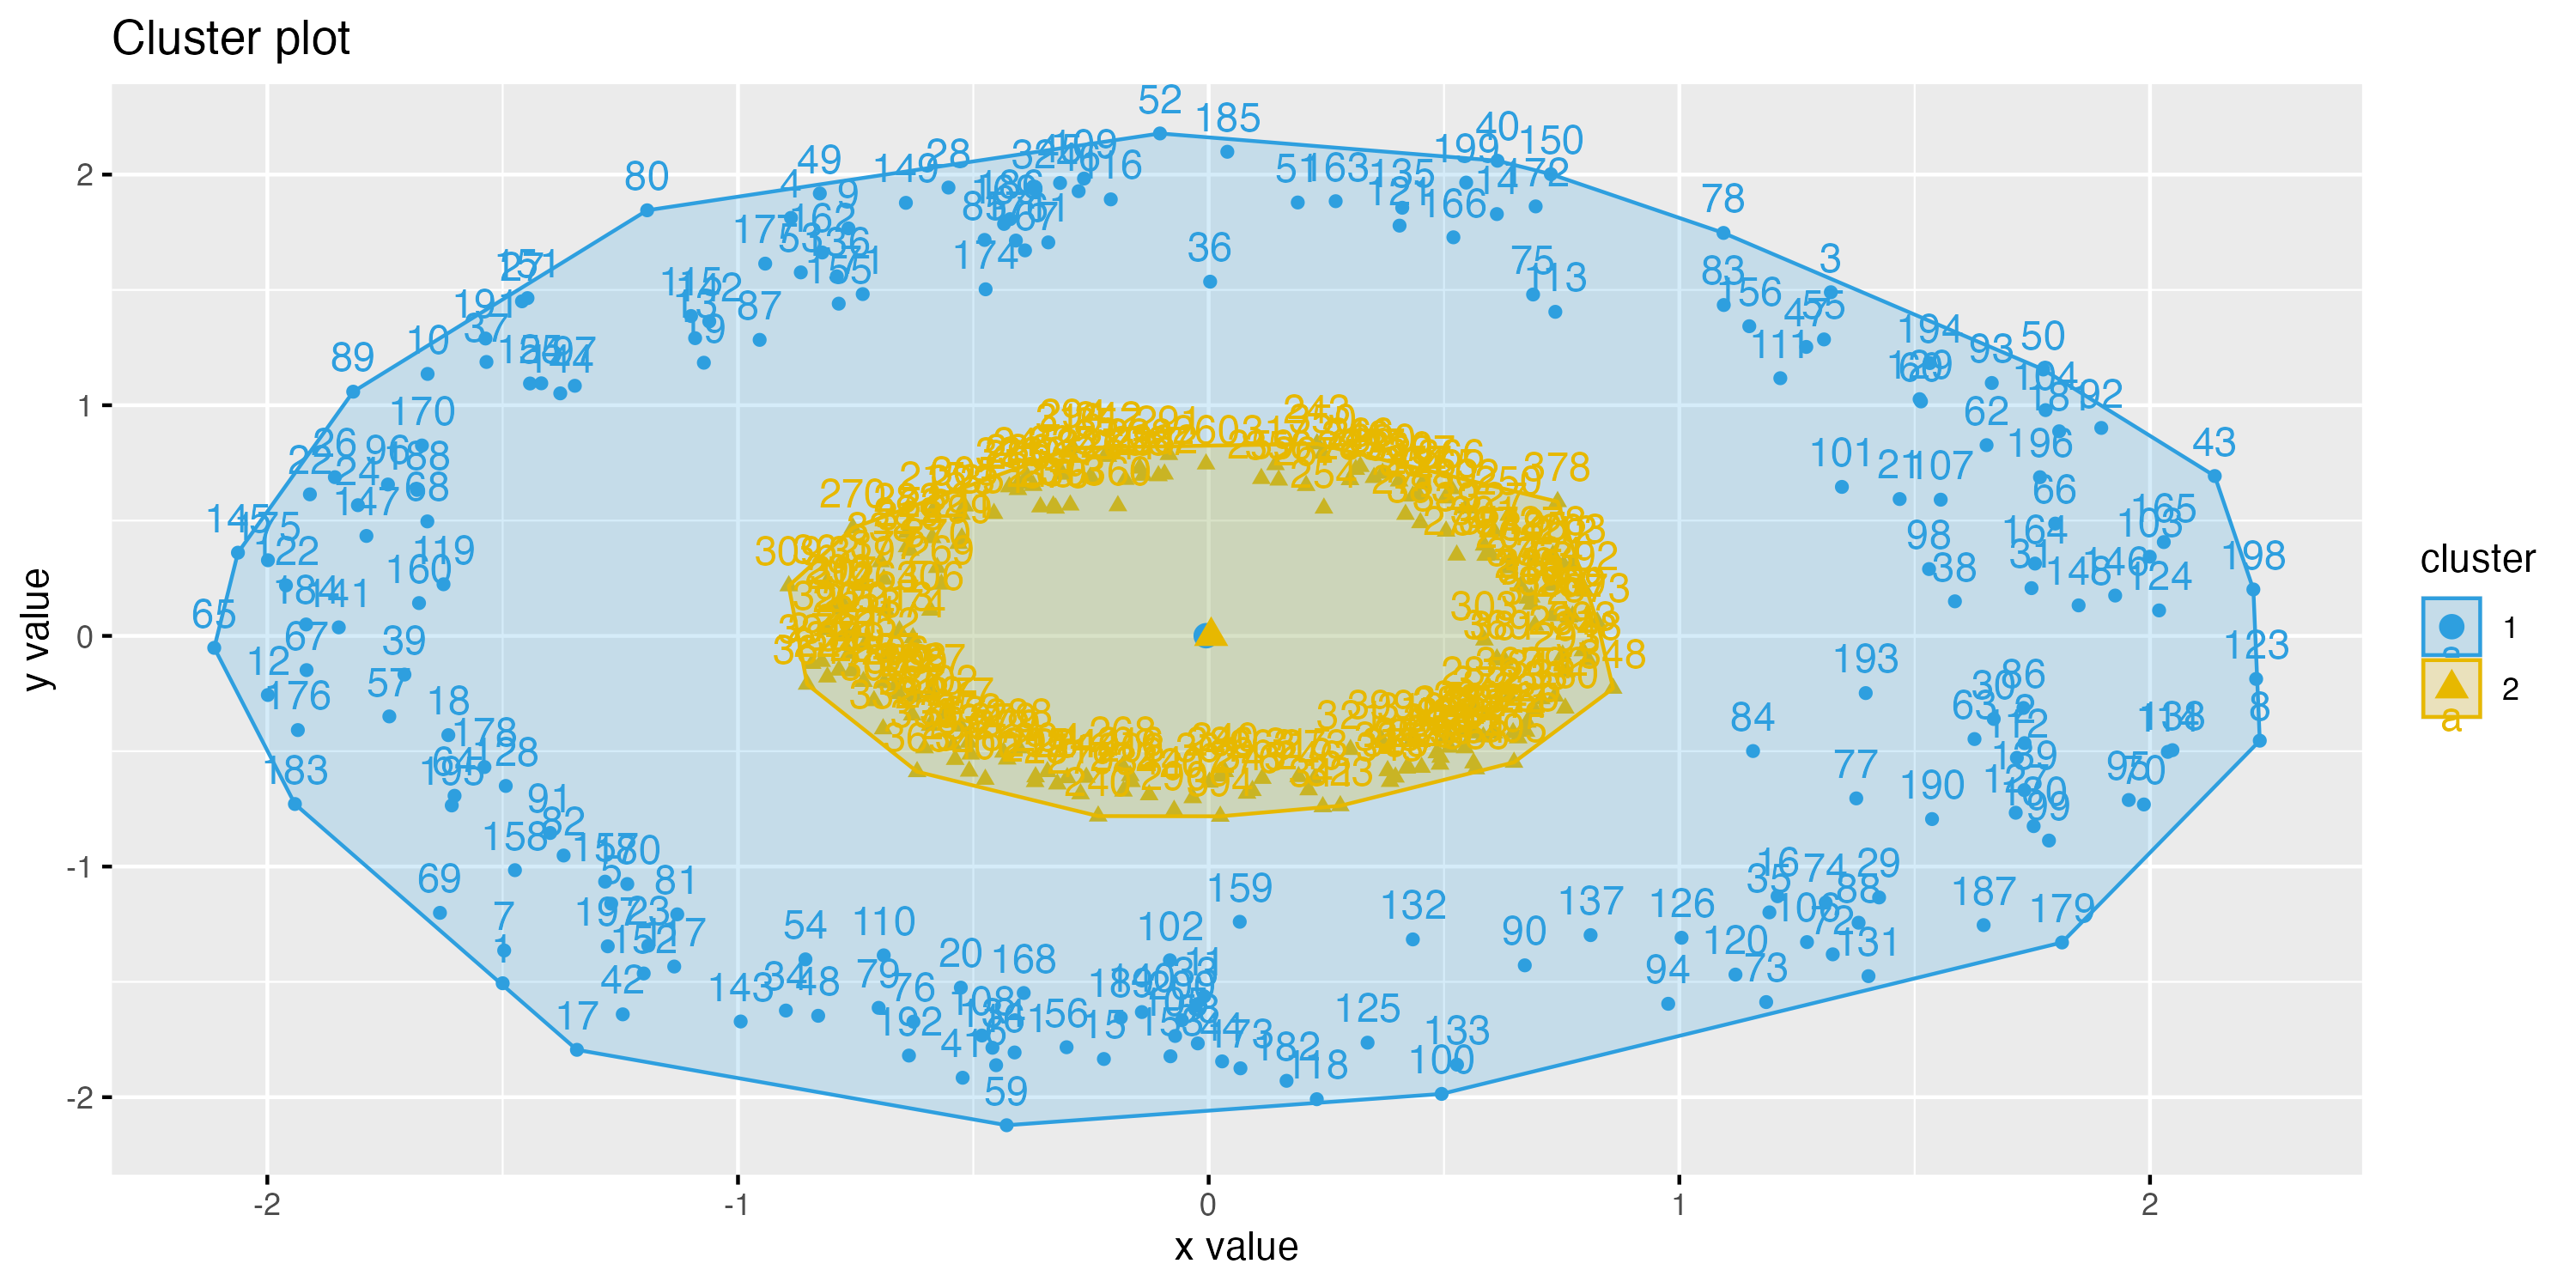
\includegraphics[keepaspectratio]{05_cluster_analysis_files/figure-beamer/unnamed-chunk-33-1.png}}
\end{column}
\end{columns}
\end{frame}

\begin{frame}{Задание 4}
\protect\phantomsection\label{ux437ux430ux434ux430ux43dux438ux435-4}
Кластеризуйте данные по волкам, используя DBSCAN-алгоритм.
\end{frame}

\begin{frame}[fragile]{Примерное решение}
\protect\phantomsection\label{ux43fux440ux438ux43cux435ux440ux43dux43eux435-ux440ux435ux448ux435ux43dux438ux435}
\begin{columns}[T]
\begin{column}{0.5\linewidth}
\begin{Shaded}
\begin{Highlighting}[]
\FunctionTok{kNNdistplot}\NormalTok{(st\_w, }\AttributeTok{k =} \DecValTok{4}\NormalTok{)}
\FunctionTok{abline}\NormalTok{(}\AttributeTok{h =} \FloatTok{2.4}\NormalTok{, }\AttributeTok{lty =} \DecValTok{2}\NormalTok{) }
\end{Highlighting}
\end{Shaded}

\pandocbounded{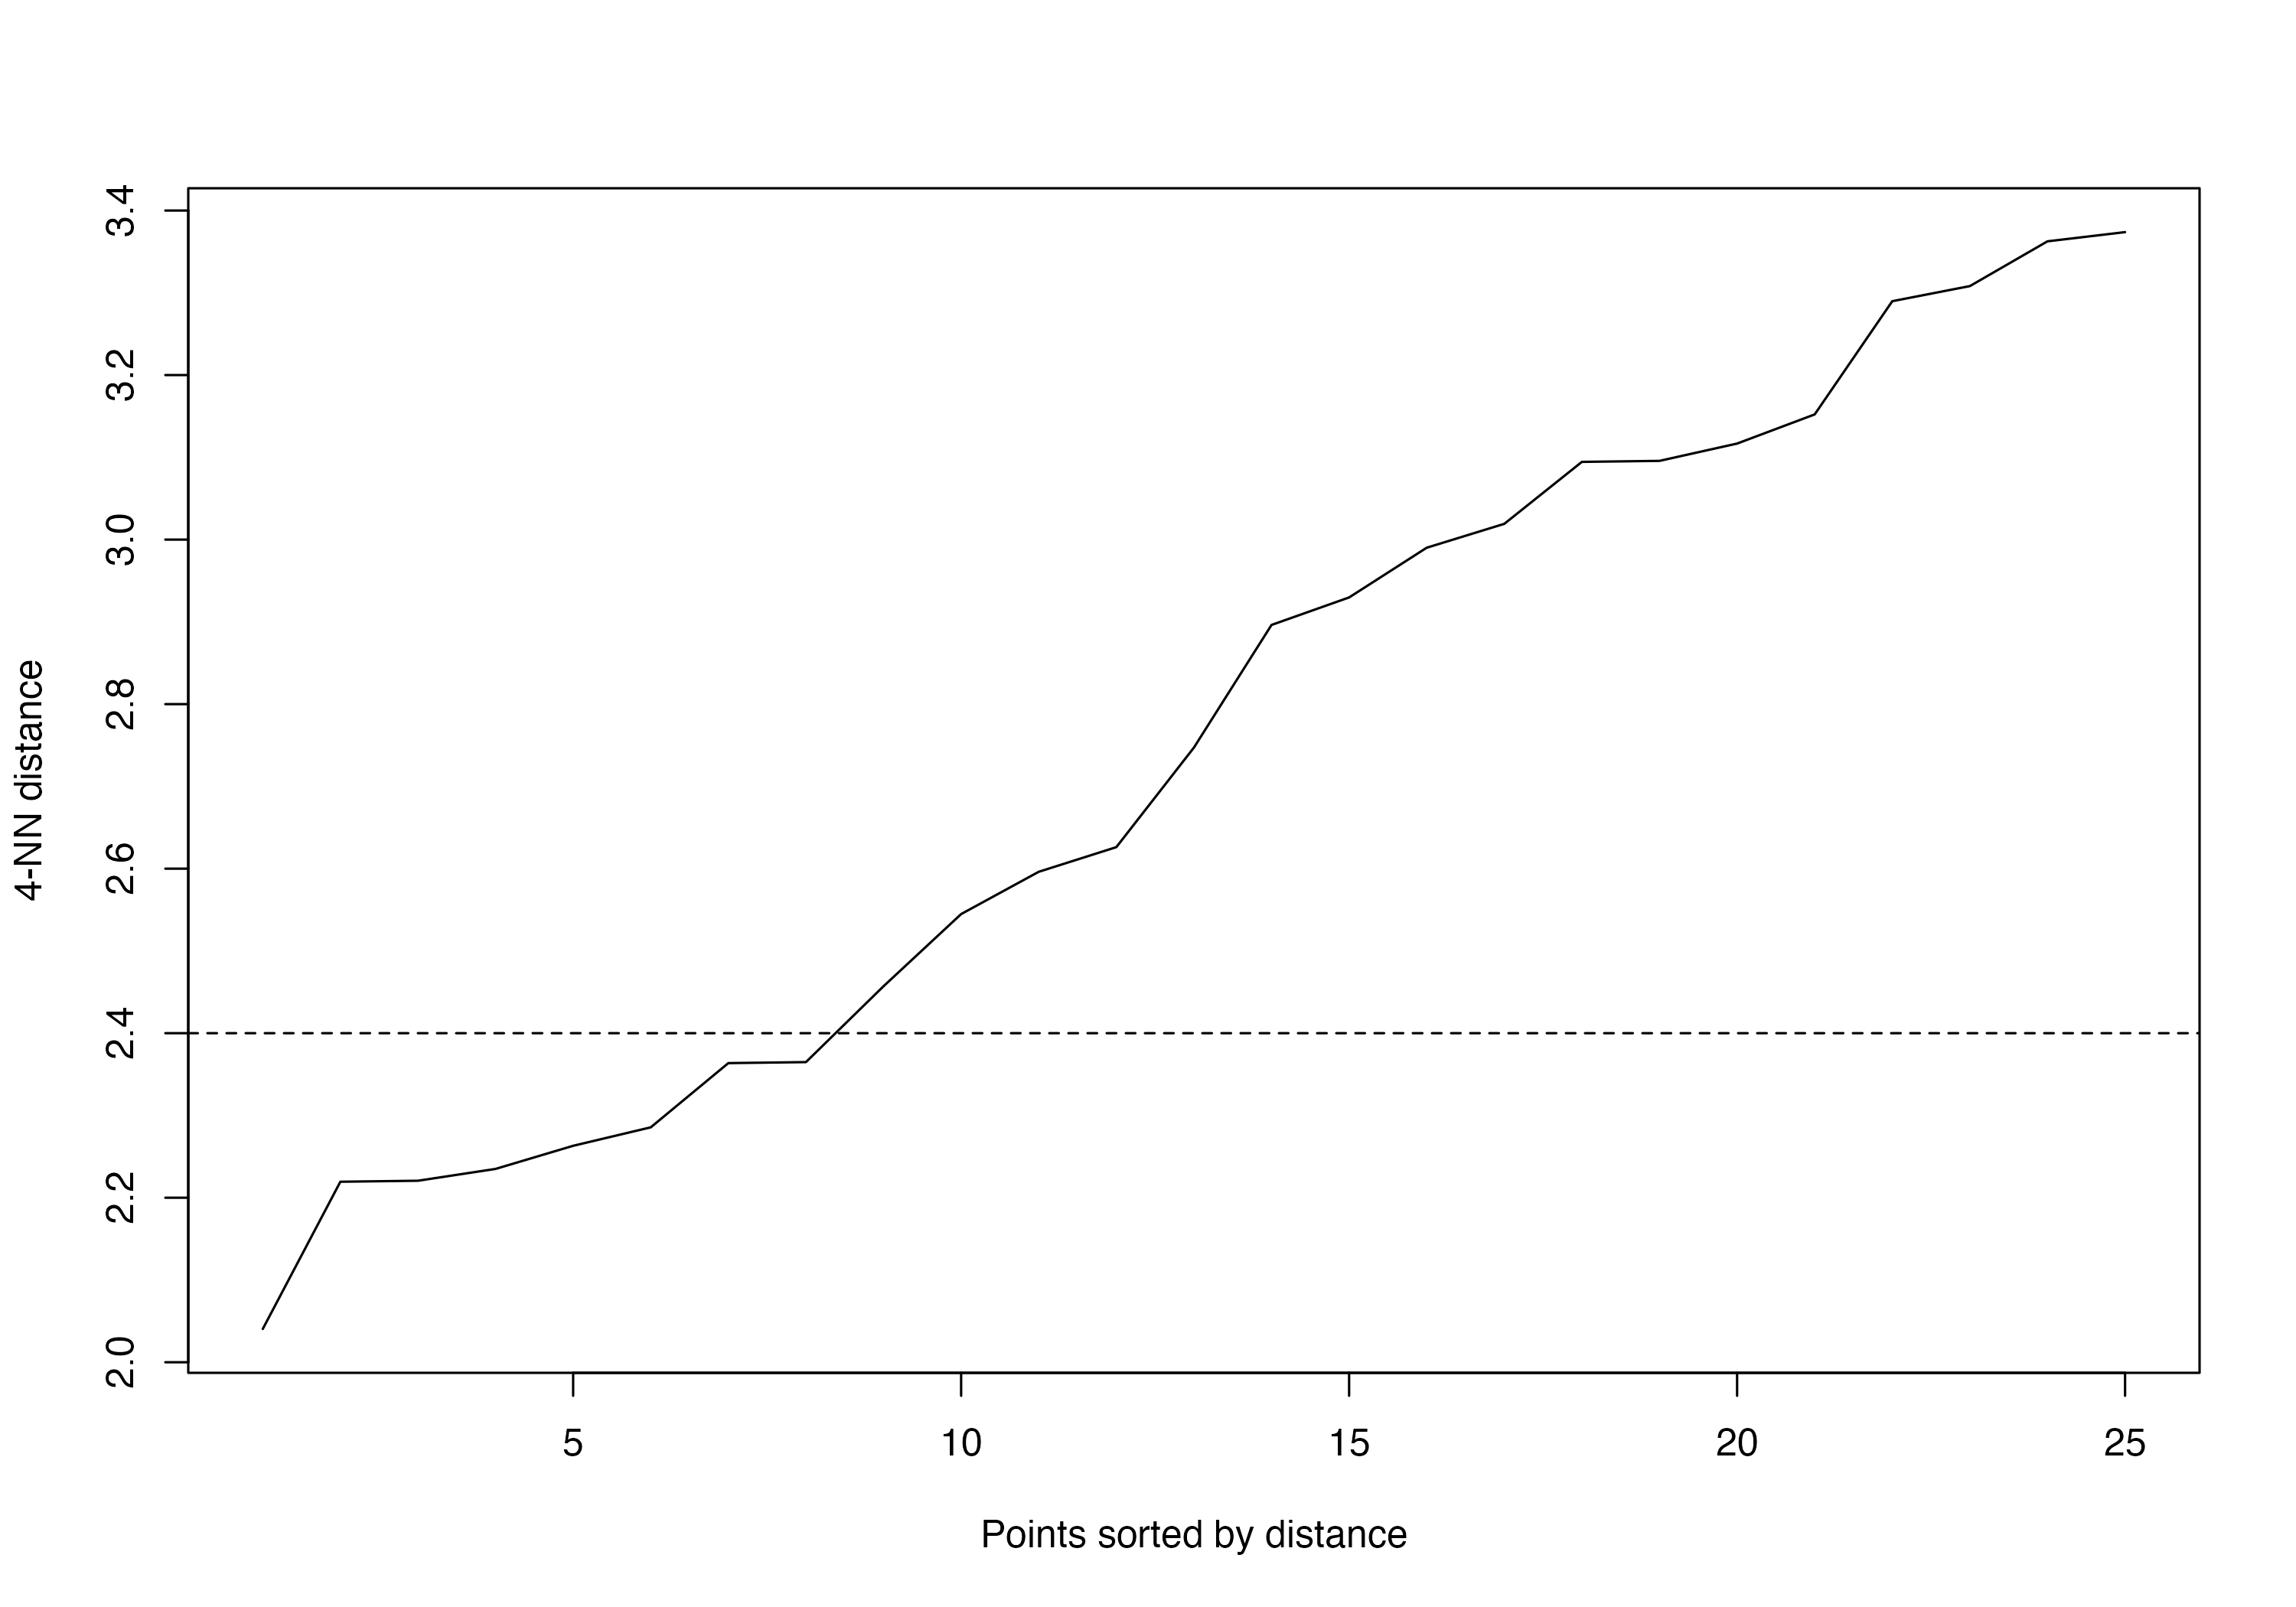
\includegraphics[keepaspectratio]{05_cluster_analysis_files/figure-beamer/unnamed-chunk-34-1.png}}
\end{column}

\begin{column}{0.5\linewidth}
\begin{Shaded}
\begin{Highlighting}[]
\NormalTok{w\_dbscan }\OtherTok{\textless{}{-}} \FunctionTok{dbscan}\NormalTok{(st\_w, }\FloatTok{2.4}\NormalTok{, }\DecValTok{4}\NormalTok{)}
\FunctionTok{fviz\_cluster}\NormalTok{(w\_dbscan, }\AttributeTok{data =}\NormalTok{ st\_w)}
\end{Highlighting}
\end{Shaded}

\pandocbounded{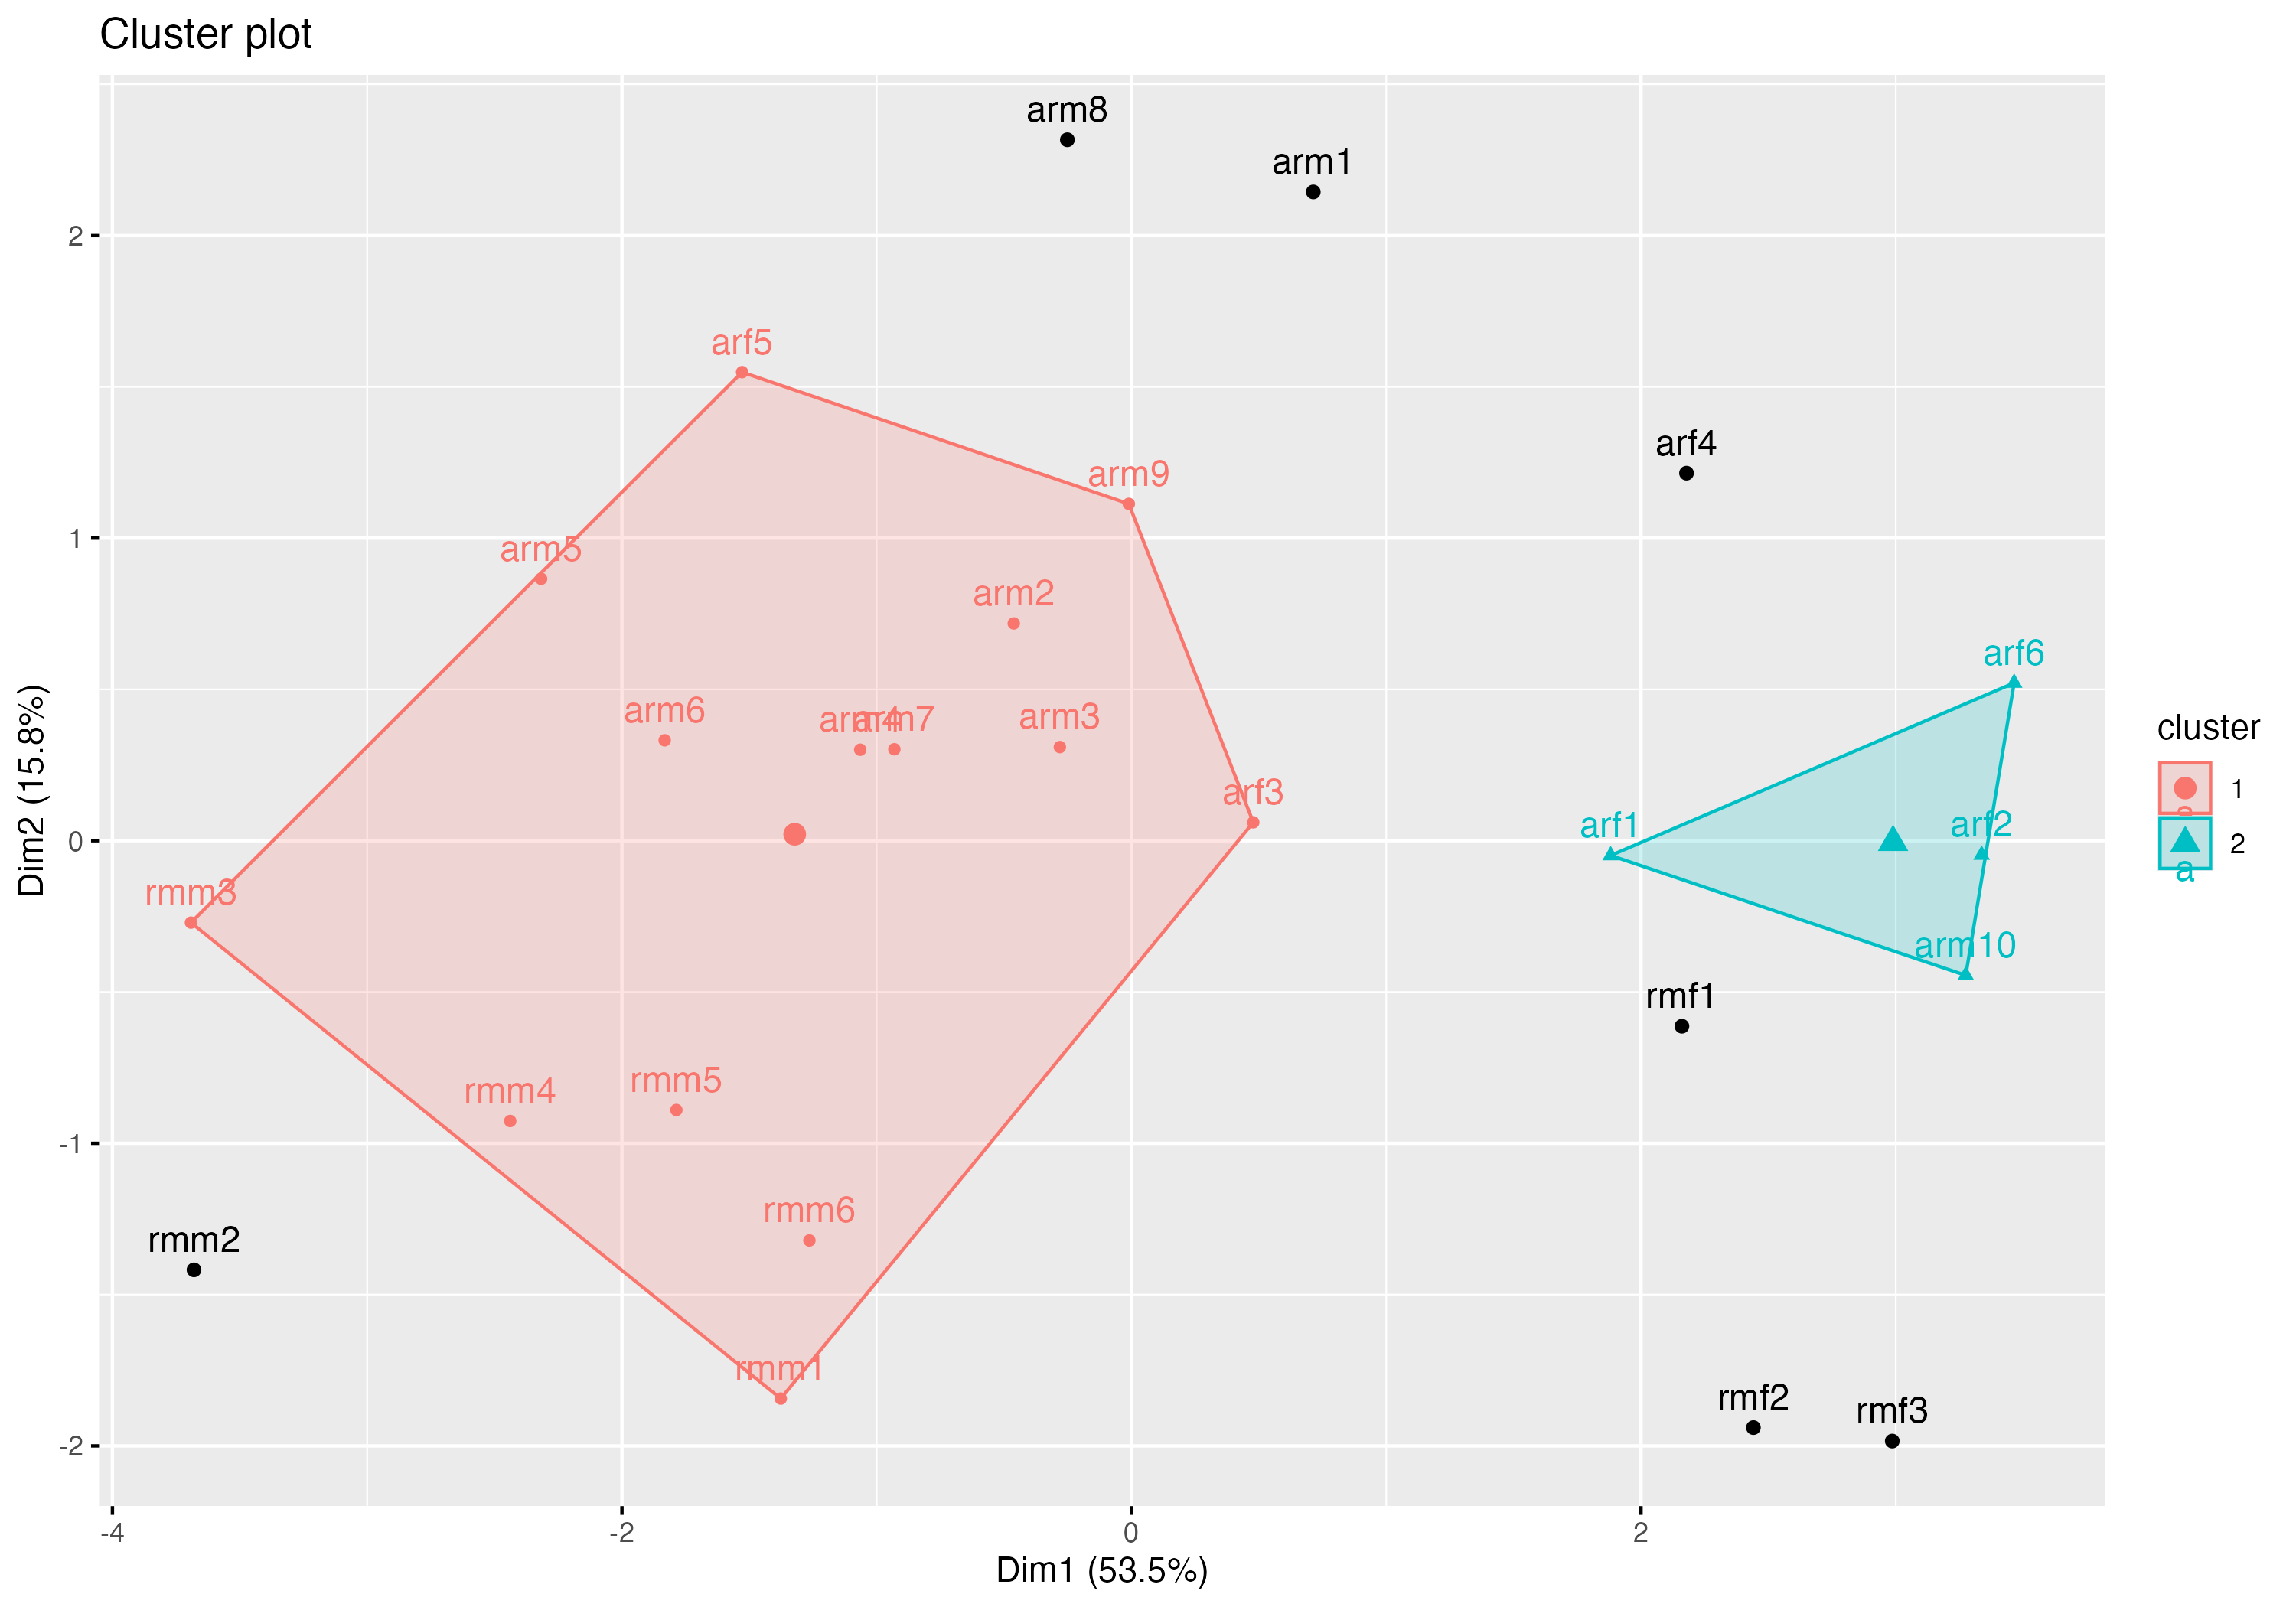
\includegraphics[keepaspectratio]{05_cluster_analysis_files/figure-beamer/unnamed-chunk-35-1.png}}
\end{column}
\end{columns}
\end{frame}

\begin{frame}{Метод нечёткой кластеризации C-средних (C-means, fuzzy
clustering)}
\protect\phantomsection\label{ux43cux435ux442ux43eux434-ux43dux435ux447ux451ux442ux43aux43eux439-ux43aux43bux430ux441ux442ux435ux440ux438ux437ux430ux446ux438ux438-c-ux441ux440ux435ux434ux43dux438ux445-c-means-fuzzy-clustering}
При данном подходе объект необязательно принадлежит одному кластеру.
Каждому объекту присваивается вероятность принадлежности к кластеру
(membership value). В сумме все значения принадлежности к кластеру дают
1 для каждого из объектов.
\end{frame}

\begin{frame}{Алгоритм C-means}
\protect\phantomsection\label{ux430ux43bux433ux43eux440ux438ux442ux43c-c-means}
\begin{enumerate}
\item
  Каждому объекту приписывается случайное значение принадлежности к
  кластеру.
\item
  Рассчитываются центроиды для каждого кластера:
\end{enumerate}

\[\hat{v}_{i} = \frac{\sum^{N}_{k=1}(\hat{u}_{ik})^{m}y_k}{\sum^{N}_{k=1}(\hat{u}_{ik})^m}\]

\scriptsize

где \(\hat{u}\) --- значение принадлежности к кластеру, \(m\) ---
параметр размытости (fuzziness), равный обычно 2, \(y_k\) --- конкретный
объект, N --- количество объектов.
\end{frame}

\begin{frame}{Алгоритм C-means}
\protect\phantomsection\label{ux430ux43bux433ux43eux440ux438ux442ux43c-c-means-1}
\begin{enumerate}
\setcounter{enumi}{2}
\item
  Расчёт расстояния от каждой точки до центроида.
\item
  Обновление значений принадлежности к кластерам.
\end{enumerate}

\scriptsize

\[\hat{u}_{ik} = (\sum^{c}_{j=1}(\frac{\hat{d}_{ik}}{\hat{d}_{jk}})^{\frac{2}{m-1}})^{-1}\]
где \(d_{ki}\) --- расстояние от точки до центроида.

\begin{enumerate}
\setcounter{enumi}{4}
\tightlist
\item
  Повторить шаги с 2 по 4, пока не будут получены постоянные значения
  принадлежности к кластеру.
\end{enumerate}
\end{frame}

\begin{frame}[fragile]{Кластеризация C-means в R}
\protect\phantomsection\label{ux43aux43bux430ux441ux442ux435ux440ux438ux437ux430ux446ux438ux44f-c-means-ux432-r}
Есть несколько функций из разных пакетов, реализующих кластеризацию
С-средних (например \texttt{fanny} из \texttt{cluster}, \texttt{cmeans}
из \texttt{e1071}, \texttt{fcm} из \texttt{ppclust} и т.д.). Мы
воспользуемся функцией \texttt{fanny} из пакета \texttt{cluster}.

Функция funny принимает как исходные данные, так и матрицу расстояний.

\tiny

\begin{Shaded}
\begin{Highlighting}[]
\NormalTok{w\_cmeans }\OtherTok{\textless{}{-}} \FunctionTok{fanny}\NormalTok{(d, }\AttributeTok{k =} \DecValTok{4}\NormalTok{, }\AttributeTok{memb.exp =} \DecValTok{2}\NormalTok{)}
\FunctionTok{summary}\NormalTok{(w\_cmeans)}
\end{Highlighting}
\end{Shaded}

\begin{verbatim}
Fuzzy Clustering object of class 'fanny' :                      
m.ship.expon.        2
objective      12.0661
tolerance        1e-15
iterations          85
converged            1
maxit              500
n                   25
Membership coefficients (in %, rounded):
      [,1] [,2] [,3] [,4]
rmm1    28   17   28   28
rmm2    28   16   28   28
rmm3    28   16   28   28
rmm4    29   14   29   29
rmm5    29   14   29   29
rmm6    28   17   28   28
rmf1    20   39   20   20
rmf2    21   37   21   21
rmf3    22   35   22   22
arm1    25   24   25   25
arm2    28   17   28   28
arm3    27   18   27   27
arm4    28   16   28   28
arm5    28   15   28   28
arm6    29   14   29   29
arm7    29   14   29   29
arm8    26   21   26   26
arm9    26   21   26   26
arm10   21   38   21   21
arf1    21   36   21   21
arf2    20   40   20   20
arf3    25   24   25   25
arf4    22   33   22   22
arf5    27   18   27   27
arf6    21   38   21   21
Fuzzyness coefficients:
dunn_coeff normalized 
0.26250519 0.01667359 
Closest hard clustering:
 rmm1  rmm2  rmm3  rmm4  rmm5  rmm6  rmf1  rmf2  rmf3  arm1  arm2  arm3  arm4 
    1     1     1     1     1     1     2     2     2     3     3     3     1 
 arm5  arm6  arm7  arm8  arm9 arm10  arf1  arf2  arf3  arf4  arf5  arf6 
    1     1     1     3     3     2     2     2     3     2     1     2 
k_crisp (= 3) < k !!

Silhouette plot information:
      cluster neighbor    sil_width
rmm4        1        3  0.364448194
rmm2        1        3  0.354518513
rmm3        1        3  0.348120151
rmm5        1        3  0.312707896
rmm1        1        3  0.290835256
arm5        1        3  0.209294464
arm6        1        3  0.190406976
rmm6        1        3  0.137320168
arf5        1        3  0.042881764
arm7        1        3 -0.001202561
arm4        1        3 -0.005208223
arf2        2        3  0.391057250
rmf2        2        3  0.347725454
arm10       2        3  0.343759126
rmf3        2        3  0.341739766
arf6        2        3  0.312071501
rmf1        2        3  0.267999826
arf1        2        3  0.200487406
arf4        2        3 -0.049650574
arm1        3        2  0.259830787
arm8        3        1  0.233975051
arm9        3        1  0.192207662
arm3        3        1  0.132852682
arf3        3        2  0.083143033
arm2        3        1  0.054878285
Average silhouette width per cluster:
[1] 0.2040111 0.2693987 0.1594813 0.2059507
Average silhouette width of total data set:
[1] 0.214248

Available components:
 [1] "membership"  "coeff"       "memb.exp"    "clustering"  "k.crisp"    
 [6] "objective"   "convergence" "diss"        "call"        "silinfo"    
\end{verbatim}
\end{frame}

\begin{frame}[fragile]{Оценка качества кластеризации: ширина силуэта}
\protect\phantomsection\label{ux43eux446ux435ux43dux43aux430-ux43aux430ux447ux435ux441ux442ux432ux430-ux43aux43bux430ux441ux442ux435ux440ux438ux437ux430ux446ux438ux438-ux448ux438ux440ux438ux43dux430-ux441ux438ux43bux443ux44dux442ux430-1}
\begin{Shaded}
\begin{Highlighting}[]
\FunctionTok{plot}\NormalTok{(}\FunctionTok{silhouette}\NormalTok{(w\_cmeans), }\AttributeTok{cex.names =} \FloatTok{0.6}\NormalTok{)}
\end{Highlighting}
\end{Shaded}

\pandocbounded{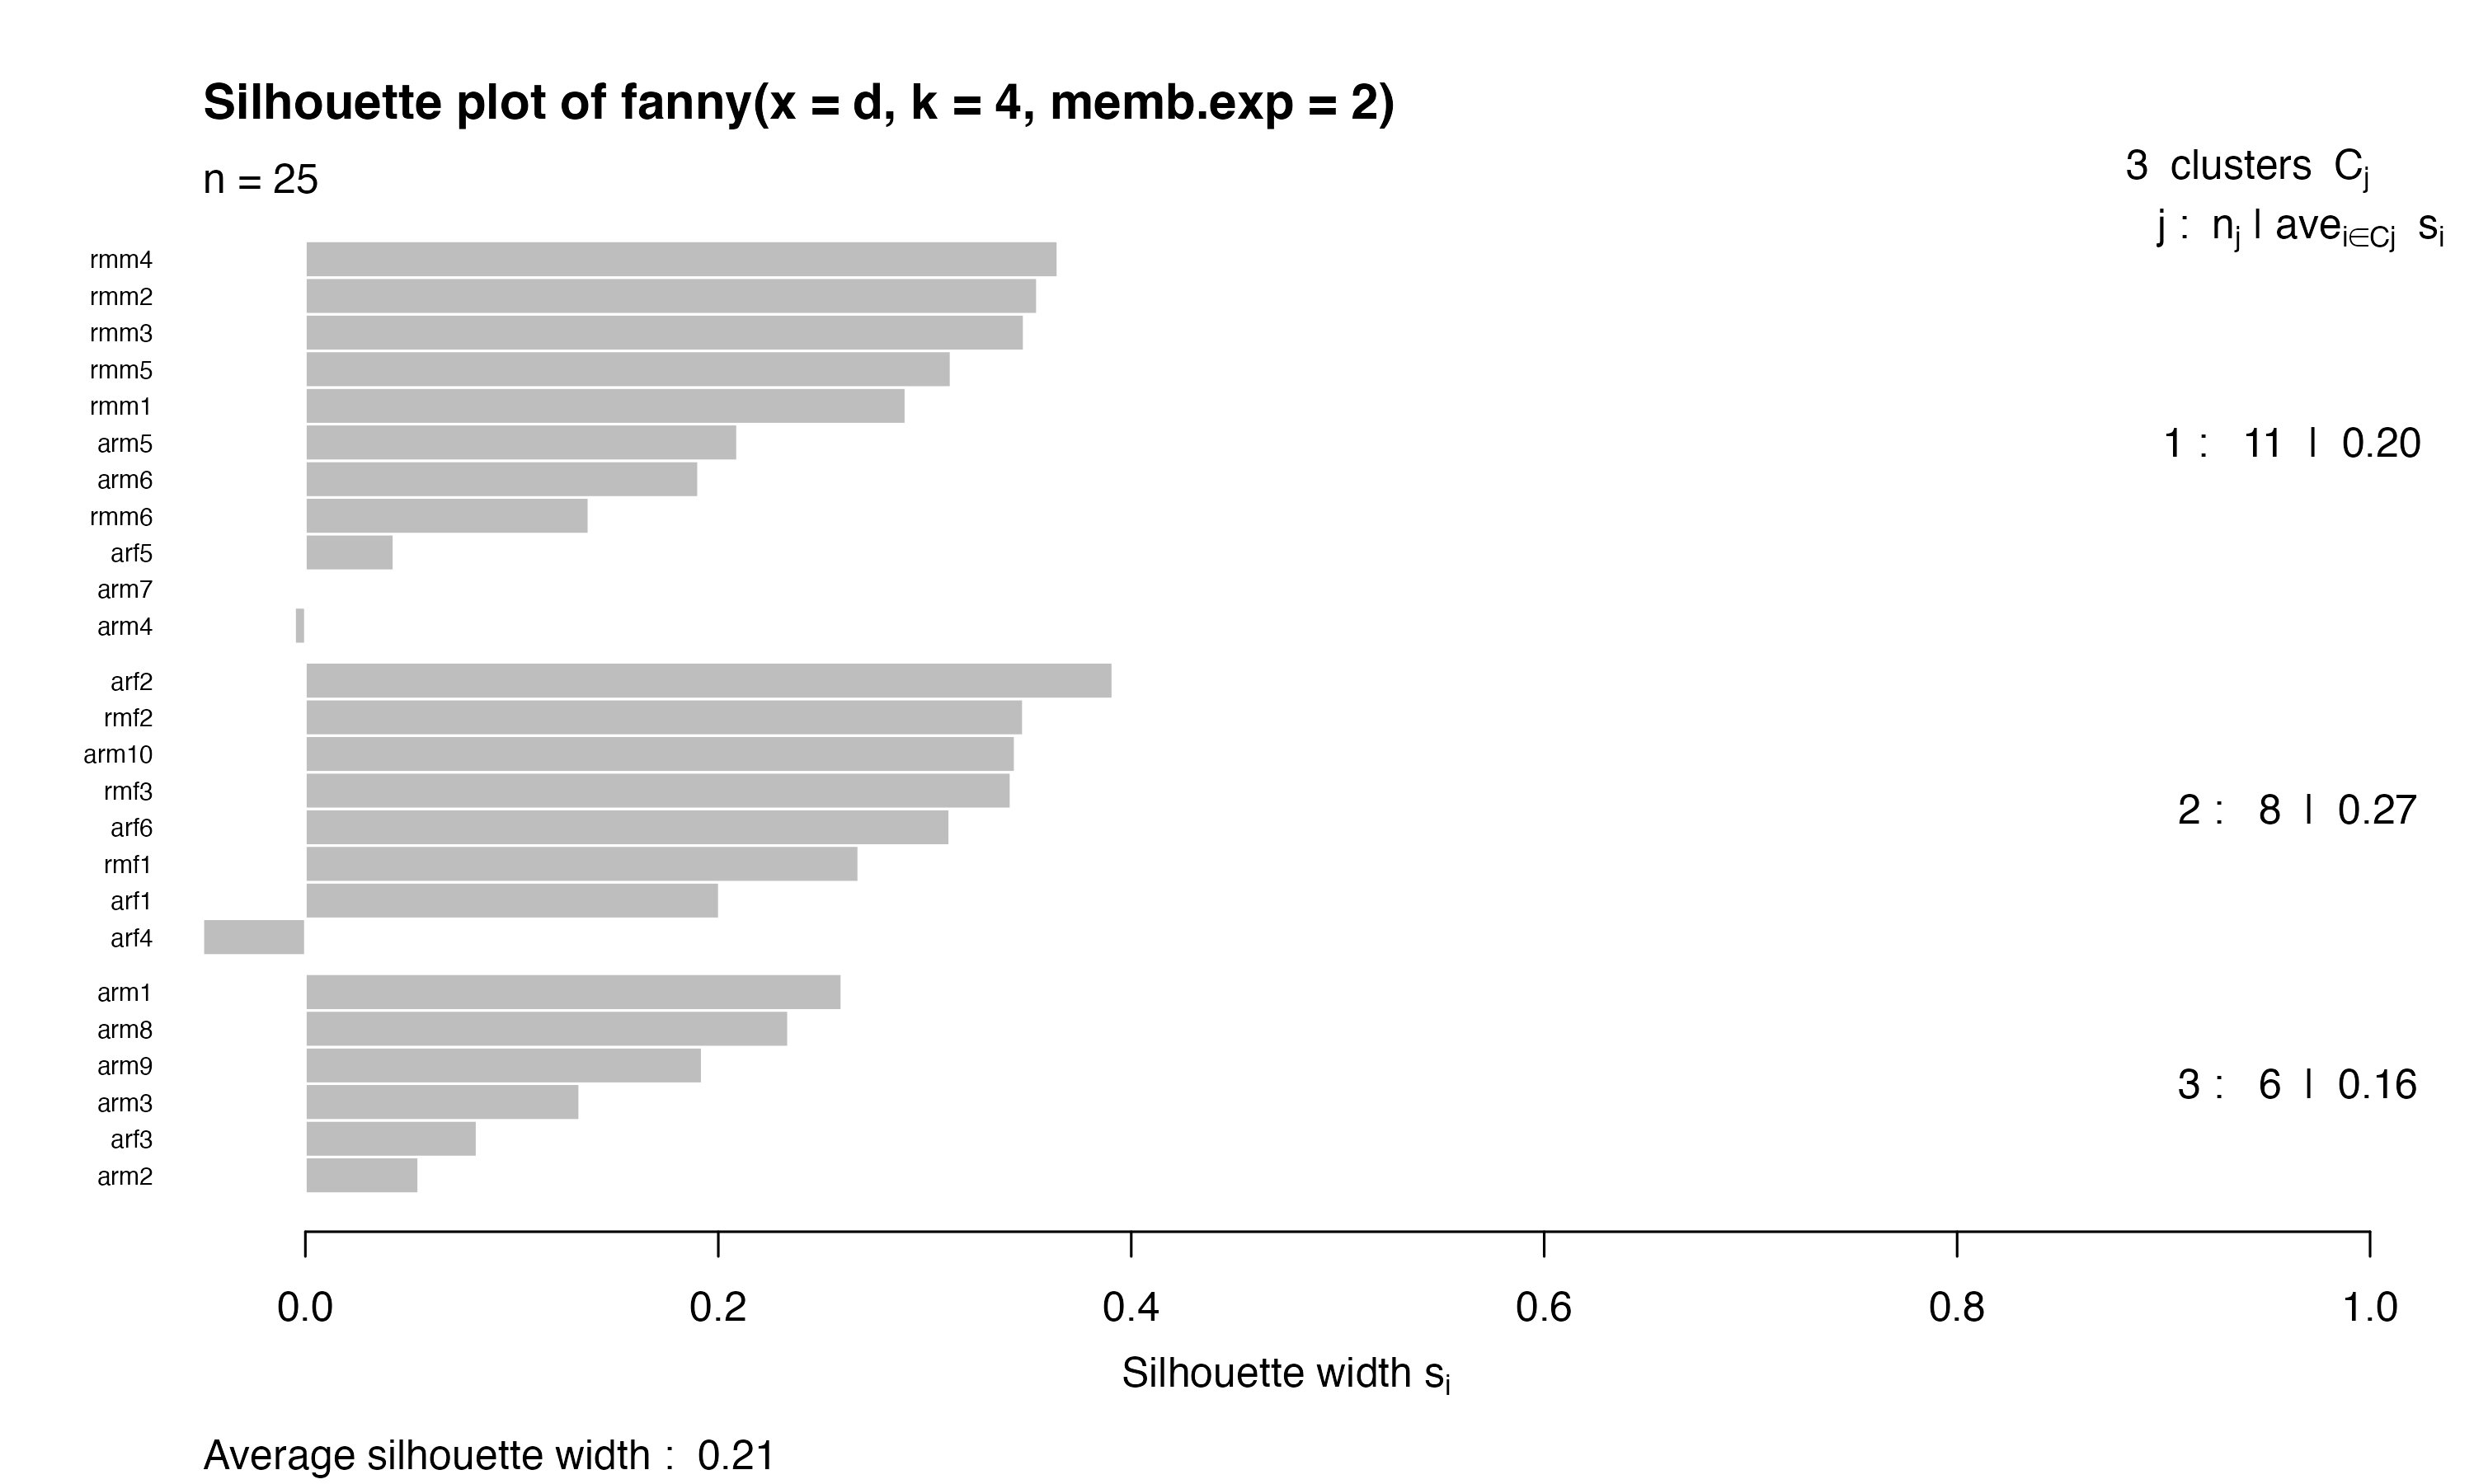
\includegraphics[keepaspectratio]{05_cluster_analysis_files/figure-beamer/unnamed-chunk-37-1.png}}
\end{frame}

\begin{frame}[fragile]{Оценка качества кластеризации: ширина силуэта}
\protect\phantomsection\label{ux43eux446ux435ux43dux43aux430-ux43aux430ux447ux435ux441ux442ux432ux430-ux43aux43bux430ux441ux442ux435ux440ux438ux437ux430ux446ux438ux438-ux448ux438ux440ux438ux43dux430-ux441ux438ux43bux443ux44dux442ux430-2}
\begin{Shaded}
\begin{Highlighting}[]
\FunctionTok{plot}\NormalTok{(}\FunctionTok{silhouette}\NormalTok{(w\_cmeans), }\AttributeTok{cex.names =} \FloatTok{0.6}\NormalTok{)}
\end{Highlighting}
\end{Shaded}

\pandocbounded{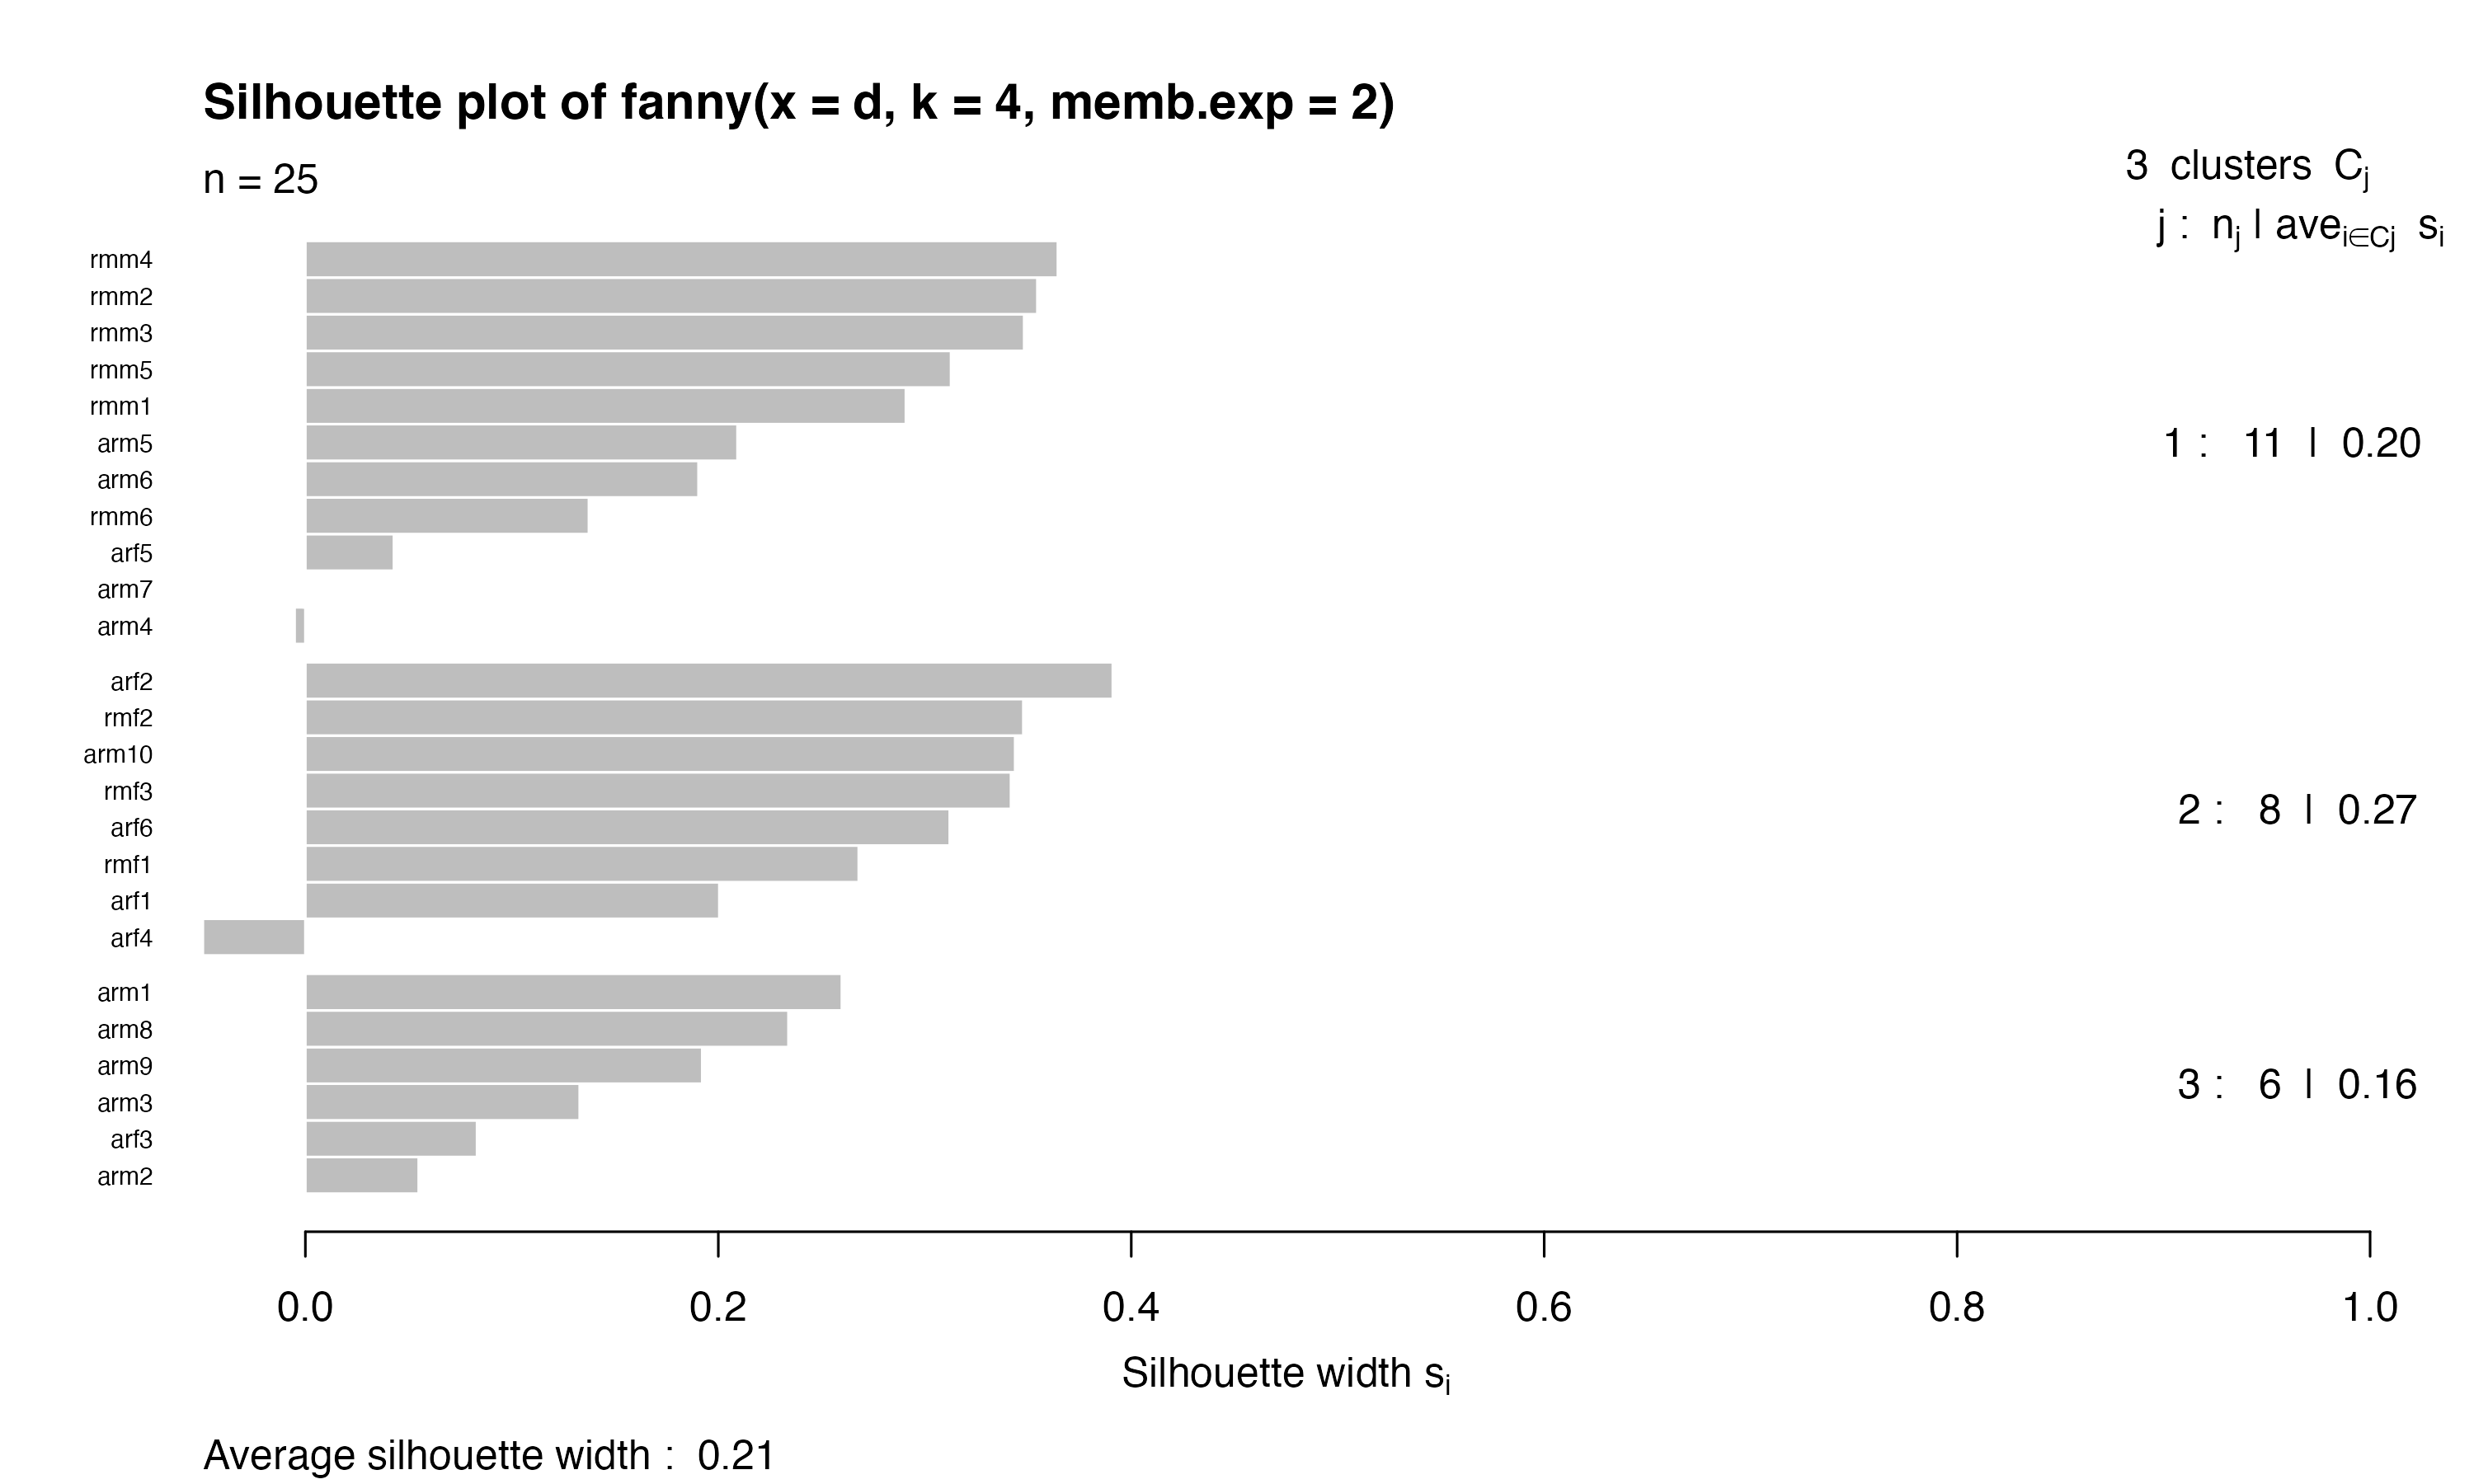
\includegraphics[keepaspectratio]{05_cluster_analysis_files/figure-beamer/unnamed-chunk-38-1.png}}

Получилась не очень качественная кластеризация.
\end{frame}

\begin{frame}{Задание 5}
\protect\phantomsection\label{ux437ux430ux434ux430ux43dux438ux435-5}
Попробуйте оценить ширину силуэта для C-means кластеризации с более
подходящим числом кластеров.
\end{frame}

\begin{frame}[fragile]{Решение}
\protect\phantomsection\label{ux440ux435ux448ux435ux43dux438ux435-3}
\begin{Shaded}
\begin{Highlighting}[]
\NormalTok{w\_2means }\OtherTok{\textless{}{-}} \FunctionTok{fanny}\NormalTok{(d, }\AttributeTok{k =} \DecValTok{2}\NormalTok{, }\AttributeTok{memb.exp =} \DecValTok{2}\NormalTok{)}
\FunctionTok{plot}\NormalTok{(}\FunctionTok{silhouette}\NormalTok{(w\_2means), }\AttributeTok{cex.names =} \FloatTok{0.6}\NormalTok{)}
\end{Highlighting}
\end{Shaded}

\pandocbounded{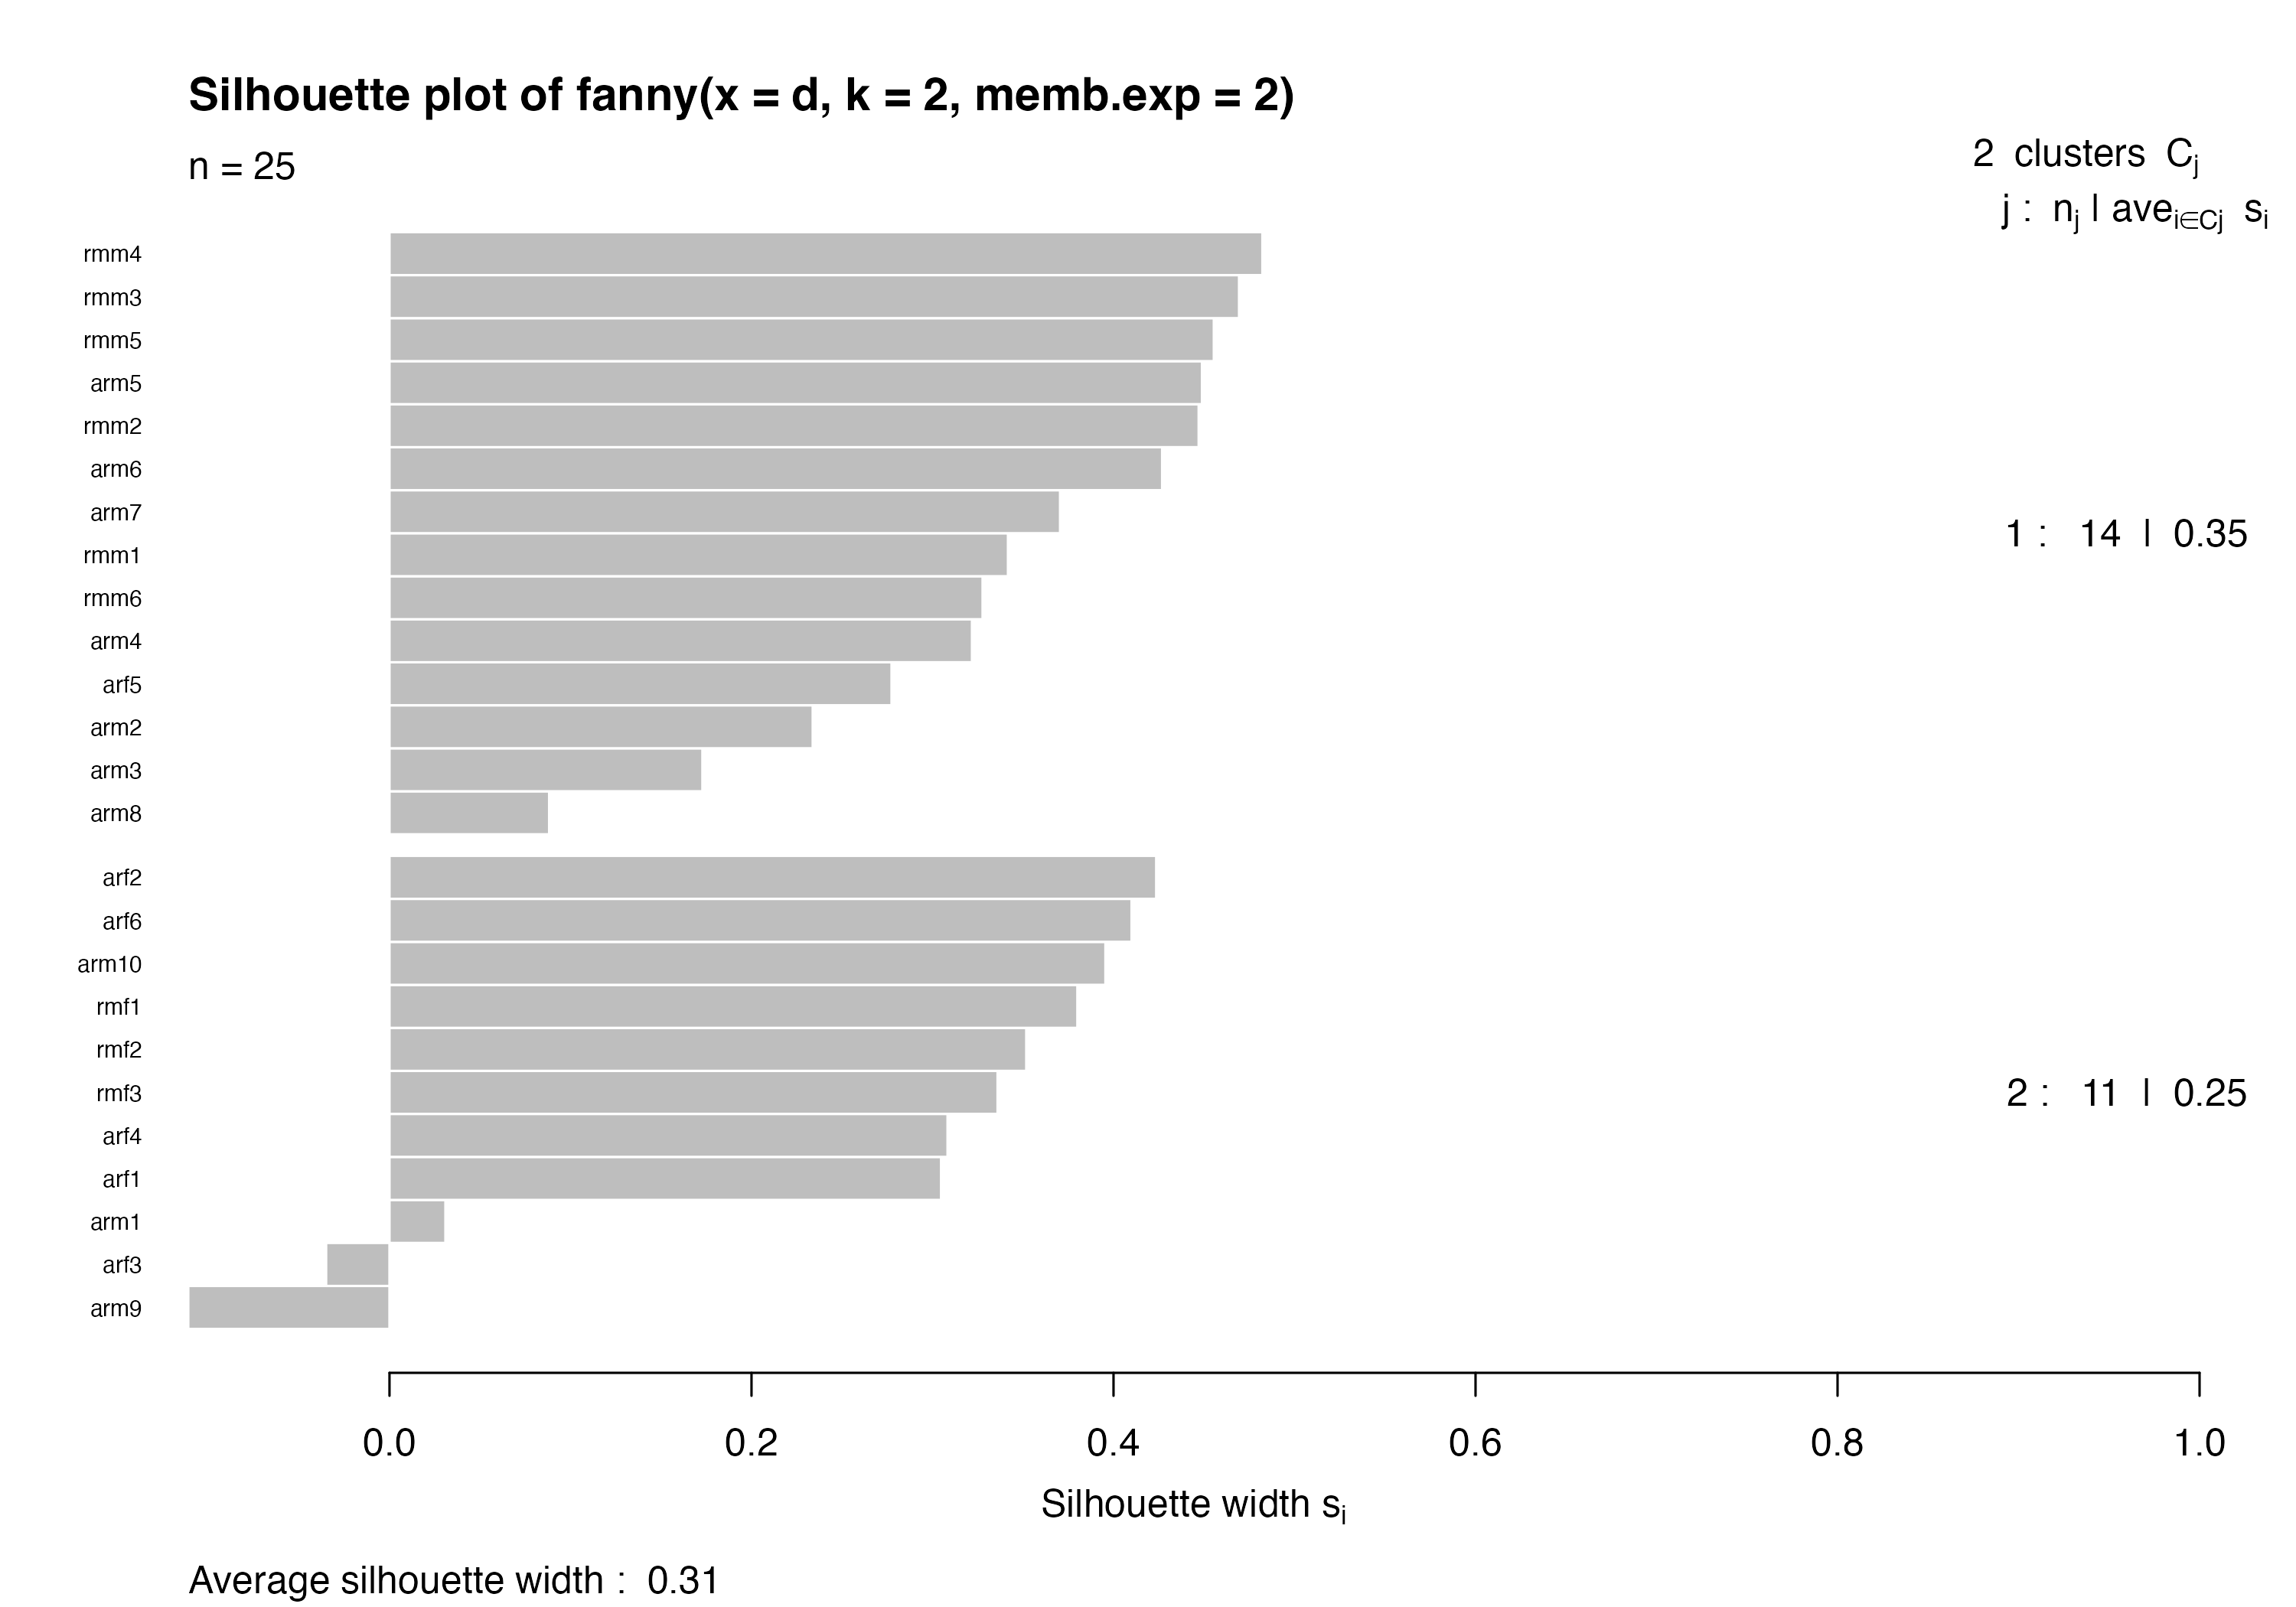
\includegraphics[keepaspectratio]{05_cluster_analysis_files/figure-beamer/unnamed-chunk-39-1.png}}
\end{frame}

\begin{frame}[fragile]{Визуализация кластеризации}
\protect\phantomsection\label{ux432ux438ux437ux443ux430ux43bux438ux437ux430ux446ux438ux44f-ux43aux43bux430ux441ux442ux435ux440ux438ux437ux430ux446ux438ux438}
Для визуализации возьмём нашу исходную ординацию nMDS.

\begin{Shaded}
\begin{Highlighting}[]
\FunctionTok{library}\NormalTok{(scatterpie)}
\NormalTok{w\_clust }\OtherTok{\textless{}{-}} \FunctionTok{cbind}\NormalTok{(dfr\_w, w\_2means}\SpecialCharTok{$}\NormalTok{membership)}
\FunctionTok{ggplot}\NormalTok{() }\SpecialCharTok{+} \FunctionTok{geom\_scatterpie}\NormalTok{(}\AttributeTok{data =}\NormalTok{ w\_clust, }\FunctionTok{aes}\NormalTok{(}\AttributeTok{x =}\NormalTok{ MDS1, }\AttributeTok{y =}\NormalTok{ MDS2),}
                           \AttributeTok{cols =} \FunctionTok{c}\NormalTok{(}\StringTok{"1"}\NormalTok{, }\StringTok{"2"}\NormalTok{))}
\end{Highlighting}
\end{Shaded}

\pandocbounded{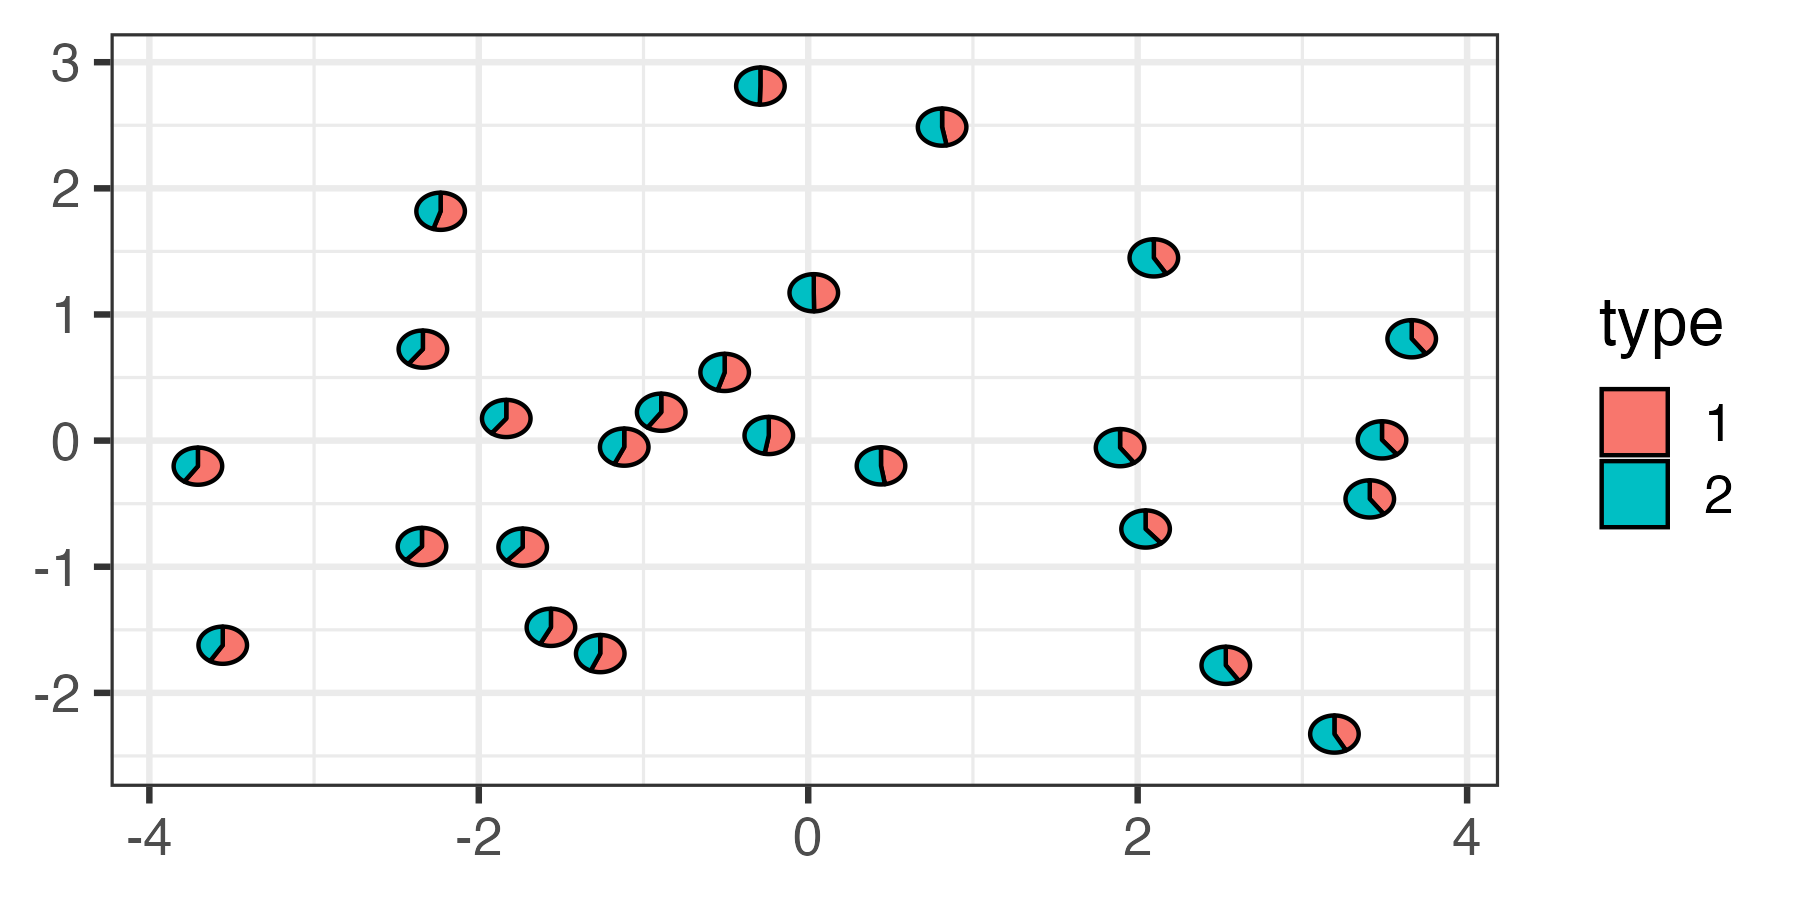
\includegraphics[keepaspectratio]{05_cluster_analysis_files/figure-beamer/unnamed-chunk-40-1.png}}
\end{frame}

\begin{frame}{Take-home messages}
\protect\phantomsection\label{take-home-messages}
\begin{itemize}
\tightlist
\item
  Результат кластеризации зависит не только от выбора коэффициента, но и
  от выбора алгоритма.
\item
  Качество кластеризации можно оценить разными способами.
\item
  Кластеризации, полученные разными методами, можно сравнить на
  танглграммах.
\end{itemize}
\end{frame}

\begin{frame}{Дополнительные ресурсы}
\protect\phantomsection\label{ux434ux43eux43fux43eux43bux43dux438ux442ux435ux43bux44cux43dux44bux435-ux440ux435ux441ux443ux440ux441ux44b}
\begin{itemize}
\tightlist
\item
  Borcard, D., Gillet, F., Legendre, P., 2011. Numerical ecology with R.
  Springer.
\item
  Legendre, P., Legendre, L., 2012. Numerical ecology. Elsevier.
\item
  Quinn, G.G.P., Keough, M.J., 2002. Experimental design and data
  analysis for biologists. Cambridge University Press.
\end{itemize}
\end{frame}

\begin{frame}{И еще ресурсы}
\protect\phantomsection\label{ux438-ux435ux449ux435-ux440ux435ux441ux443ux440ux441ux44b}
Как работает UPGMA можно посмотреть здесь:

\begin{itemize}
\tightlist
\item
  http://www.southampton.ac.uk/\textasciitilde re1u06/teaching/upgma/
\end{itemize}

Как считать поддержку ветвей (пакет + статья):

\begin{itemize}
\tightlist
\item
  pvclust: An R package for hierarchical clustering with p-values {[}WWW
  Document{]}, n.d. URL
  http://www.sigmath.es.osaka-u.ac.jp/shimo-lab/prog/pvclust/ (accessed
  11.7.14).
\end{itemize}

Для анализа молекулярных данных:

\begin{itemize}
\tightlist
\item
  Paradis, E., 2011. Analysis of Phylogenetics and Evolution with R.
  Springer.
\end{itemize}

Статья про C-means кластеризацию:

\begin{itemize}
\tightlist
\item
  Bezdek et al., 1984. FCM: The Fuzzy c-Means Clustering Algorithm.
  \emph{Computer \& Geosciences, 10: 2-3}, 191-203.
\end{itemize}
\end{frame}

\begin{frame}{Данные для самостоятельной работы}
\protect\phantomsection\label{ux434ux430ux43dux43dux44bux435-ux434ux43bux44f-ux441ux430ux43cux43eux441ux442ux43eux44fux442ux435ux43bux44cux43dux43eux439-ux440ux430ux431ux43eux442ux44b}
\textbf{Фораминиферы маршей Белого моря (Golikova et al.~2020)}

\pandocbounded{\includegraphics[keepaspectratio]{images/Golikova_etal_2020_Fig1.png}}
\end{frame}

\begin{frame}{Фораминиферы маршей Белого моря}
\protect\phantomsection\label{ux444ux43eux440ux430ux43cux438ux43dux438ux444ux435ux440ux44b-ux43cux430ux440ux448ux435ux439-ux431ux435ux43bux43eux433ux43e-ux43cux43eux440ux44f}
\pandocbounded{\includegraphics[keepaspectratio]{images/Golikova_etal_2020_fig2.png}}
\end{frame}

\begin{frame}{Фораминиферы маршей Белого моря}
\protect\phantomsection\label{ux444ux43eux440ux430ux43cux438ux43dux438ux444ux435ux440ux44b-ux43cux430ux440ux448ux435ux439-ux431ux435ux43bux43eux433ux43e-ux43cux43eux440ux44f-1}
\begin{columns}[T]
\begin{column}{0.5\linewidth}
\pandocbounded{\includegraphics[keepaspectratio]{images/Golikova_etal_2020_plate1.png}}
\end{column}

\begin{column}{0.55\linewidth}
Plate 1.

\begin{enumerate}
\tightlist
\item
  \emph{Balticammina pseudomacrescens}.
\item
  \emph{Ammotium salsum}.
\item
  \emph{Jadammina macrescens}.
\item
  \emph{Trochammina inflata}.
\item
  \emph{Ammobaculites balkwilli?}
\item
  \emph{Miliammina fusca}.
\item
  \emph{Ovammina opaca}.
\item
  \emph{Elphidium albiumbilicatum}.
\item
  \emph{Elphidium williamsoni}.
\end{enumerate}

Scale bar 500 μm.
\end{column}
\end{columns}
\end{frame}

\begin{frame}{Задание}
\protect\phantomsection\label{ux437ux430ux434ux430ux43dux438ux435-3}
Проанализируйте данные об относительных обилиях фораминифер в пробах на
Белом море.

\begin{itemize}
\item
  Выберите и обоснуйте трансформацию данных и расстояние.
\item
  Постройте ординацию nMDS по относительным обилиям фораминифер:

  \begin{itemize}
  \tightlist
  \item
    цвет значков --- растение-доминант,
  \item
    форма значков --- точка сбора.
  \end{itemize}
\item
  Постройте дендрограмму проб по сходству относительных обилий
  фораминифер.

  \begin{itemize}
  \tightlist
  \item
    оцените при помощи кофенетической корреляции, какой метод аггрегации
    лучше,
  \end{itemize}
\item
  Постройте визуализацию для методов неиерархической кластеризации
\item
  Опишите получившиеся кластеры при помощи различных параметров:

  \begin{itemize}
  \tightlist
  \item
    ширина силуэта
  \item
    бутстреп-поддержка ветвлений
  \end{itemize}
\end{itemize}
\end{frame}

\begin{frame}{Фораминиферы маршей Белого моря}
\protect\phantomsection\label{ux444ux43eux440ux430ux43cux438ux43dux438ux444ux435ux440ux44b-ux43cux430ux440ux448ux435ux439-ux431ux435ux43bux43eux433ux43e-ux43cux43eux440ux44f-2}
\centering

\includegraphics[width=0.8\linewidth,height=\textheight,keepaspectratio]{images/Golikova_etal_2020_fig5.png}
\end{frame}

\begin{frame}{Фораминиферы маршей Белого моря}
\protect\phantomsection\label{ux444ux43eux440ux430ux43cux438ux43dux438ux444ux435ux440ux44b-ux43cux430ux440ux448ux435ux439-ux431ux435ux43bux43eux433ux43e-ux43cux43eux440ux44f-3}
\pandocbounded{\includegraphics[keepaspectratio]{images/Golikova_etal_2020_fig6.png}}
\end{frame}




\end{document}
